\documentclass[]{book}
\usepackage{lmodern}
\usepackage{amssymb,amsmath}
\usepackage{ifxetex,ifluatex}
\usepackage{fixltx2e} % provides \textsubscript
\ifnum 0\ifxetex 1\fi\ifluatex 1\fi=0 % if pdftex
  \usepackage[T1]{fontenc}
  \usepackage[utf8]{inputenc}
\else % if luatex or xelatex
  \ifxetex
    \usepackage{mathspec}
  \else
    \usepackage{fontspec}
  \fi
  \defaultfontfeatures{Ligatures=TeX,Scale=MatchLowercase}
\fi
% use upquote if available, for straight quotes in verbatim environments
\IfFileExists{upquote.sty}{\usepackage{upquote}}{}
% use microtype if available
\IfFileExists{microtype.sty}{%
\usepackage{microtype}
\UseMicrotypeSet[protrusion]{basicmath} % disable protrusion for tt fonts
}{}
\usepackage{hyperref}
\hypersetup{unicode=true,
            pdftitle={PLSC 31101: Introduction To Computational Tools And Techniques For Social Research},
            pdfauthor={Rochelle Terman},
            pdfborder={0 0 0},
            breaklinks=true}
\urlstyle{same}  % don't use monospace font for urls
\usepackage{natbib}
\bibliographystyle{apalike}
\usepackage{color}
\usepackage{fancyvrb}
\newcommand{\VerbBar}{|}
\newcommand{\VERB}{\Verb[commandchars=\\\{\}]}
\DefineVerbatimEnvironment{Highlighting}{Verbatim}{commandchars=\\\{\}}
% Add ',fontsize=\small' for more characters per line
\usepackage{framed}
\definecolor{shadecolor}{RGB}{248,248,248}
\newenvironment{Shaded}{\begin{snugshade}}{\end{snugshade}}
\newcommand{\KeywordTok}[1]{\textcolor[rgb]{0.13,0.29,0.53}{\textbf{#1}}}
\newcommand{\DataTypeTok}[1]{\textcolor[rgb]{0.13,0.29,0.53}{#1}}
\newcommand{\DecValTok}[1]{\textcolor[rgb]{0.00,0.00,0.81}{#1}}
\newcommand{\BaseNTok}[1]{\textcolor[rgb]{0.00,0.00,0.81}{#1}}
\newcommand{\FloatTok}[1]{\textcolor[rgb]{0.00,0.00,0.81}{#1}}
\newcommand{\ConstantTok}[1]{\textcolor[rgb]{0.00,0.00,0.00}{#1}}
\newcommand{\CharTok}[1]{\textcolor[rgb]{0.31,0.60,0.02}{#1}}
\newcommand{\SpecialCharTok}[1]{\textcolor[rgb]{0.00,0.00,0.00}{#1}}
\newcommand{\StringTok}[1]{\textcolor[rgb]{0.31,0.60,0.02}{#1}}
\newcommand{\VerbatimStringTok}[1]{\textcolor[rgb]{0.31,0.60,0.02}{#1}}
\newcommand{\SpecialStringTok}[1]{\textcolor[rgb]{0.31,0.60,0.02}{#1}}
\newcommand{\ImportTok}[1]{#1}
\newcommand{\CommentTok}[1]{\textcolor[rgb]{0.56,0.35,0.01}{\textit{#1}}}
\newcommand{\DocumentationTok}[1]{\textcolor[rgb]{0.56,0.35,0.01}{\textbf{\textit{#1}}}}
\newcommand{\AnnotationTok}[1]{\textcolor[rgb]{0.56,0.35,0.01}{\textbf{\textit{#1}}}}
\newcommand{\CommentVarTok}[1]{\textcolor[rgb]{0.56,0.35,0.01}{\textbf{\textit{#1}}}}
\newcommand{\OtherTok}[1]{\textcolor[rgb]{0.56,0.35,0.01}{#1}}
\newcommand{\FunctionTok}[1]{\textcolor[rgb]{0.00,0.00,0.00}{#1}}
\newcommand{\VariableTok}[1]{\textcolor[rgb]{0.00,0.00,0.00}{#1}}
\newcommand{\ControlFlowTok}[1]{\textcolor[rgb]{0.13,0.29,0.53}{\textbf{#1}}}
\newcommand{\OperatorTok}[1]{\textcolor[rgb]{0.81,0.36,0.00}{\textbf{#1}}}
\newcommand{\BuiltInTok}[1]{#1}
\newcommand{\ExtensionTok}[1]{#1}
\newcommand{\PreprocessorTok}[1]{\textcolor[rgb]{0.56,0.35,0.01}{\textit{#1}}}
\newcommand{\AttributeTok}[1]{\textcolor[rgb]{0.77,0.63,0.00}{#1}}
\newcommand{\RegionMarkerTok}[1]{#1}
\newcommand{\InformationTok}[1]{\textcolor[rgb]{0.56,0.35,0.01}{\textbf{\textit{#1}}}}
\newcommand{\WarningTok}[1]{\textcolor[rgb]{0.56,0.35,0.01}{\textbf{\textit{#1}}}}
\newcommand{\AlertTok}[1]{\textcolor[rgb]{0.94,0.16,0.16}{#1}}
\newcommand{\ErrorTok}[1]{\textcolor[rgb]{0.64,0.00,0.00}{\textbf{#1}}}
\newcommand{\NormalTok}[1]{#1}
\usepackage{longtable,booktabs}
\usepackage{graphicx,grffile}
\makeatletter
\def\maxwidth{\ifdim\Gin@nat@width>\linewidth\linewidth\else\Gin@nat@width\fi}
\def\maxheight{\ifdim\Gin@nat@height>\textheight\textheight\else\Gin@nat@height\fi}
\makeatother
% Scale images if necessary, so that they will not overflow the page
% margins by default, and it is still possible to overwrite the defaults
% using explicit options in \includegraphics[width, height, ...]{}
\setkeys{Gin}{width=\maxwidth,height=\maxheight,keepaspectratio}
\IfFileExists{parskip.sty}{%
\usepackage{parskip}
}{% else
\setlength{\parindent}{0pt}
\setlength{\parskip}{6pt plus 2pt minus 1pt}
}
\setlength{\emergencystretch}{3em}  % prevent overfull lines
\providecommand{\tightlist}{%
  \setlength{\itemsep}{0pt}\setlength{\parskip}{0pt}}
\setcounter{secnumdepth}{5}
% Redefines (sub)paragraphs to behave more like sections
\ifx\paragraph\undefined\else
\let\oldparagraph\paragraph
\renewcommand{\paragraph}[1]{\oldparagraph{#1}\mbox{}}
\fi
\ifx\subparagraph\undefined\else
\let\oldsubparagraph\subparagraph
\renewcommand{\subparagraph}[1]{\oldsubparagraph{#1}\mbox{}}
\fi

%%% Use protect on footnotes to avoid problems with footnotes in titles
\let\rmarkdownfootnote\footnote%
\def\footnote{\protect\rmarkdownfootnote}

%%% Change title format to be more compact
\usepackage{titling}

% Create subtitle command for use in maketitle
\providecommand{\subtitle}[1]{
  \posttitle{
    \begin{center}\large#1\end{center}
    }
}

\setlength{\droptitle}{-2em}

  \title{PLSC 31101: Introduction To Computational Tools And Techniques For
Social Research}
    \pretitle{\vspace{\droptitle}\centering\huge}
  \posttitle{\par}
    \author{Rochelle Terman}
    \preauthor{\centering\large\emph}
  \postauthor{\par}
      \predate{\centering\large\emph}
  \postdate{\par}
    \date{2019-09-18}

\usepackage{booktabs}

\begin{document}
\maketitle

{
\setcounter{tocdepth}{1}
\tableofcontents
}
\part{Before Class}\label{part-before-class}

\chapter{Syllabus}\label{syllabus}

\begin{itemize}
\item
  Instructor: \href{http://rochelleterman.com/}{Rochelle Terman},
  \href{mailto:rterman@uchicago.edu}{\nolinkurl{rterman@uchicago.edu}}
\item
  TA: Pete Cuppernull,
  \href{mailto:pcuppernull@uchicago.edu}{\nolinkurl{pcuppernull@uchicago.edu}}
\item
  Time: Tuesdays and Thursdays, 12:30 pm -- 1:50 pm
\item
  Place: Cobb Hall 303
\item
  Office hours:

  \begin{itemize}
  \tightlist
  \item
    Rochelle Terman: TBA
  \item
    Pete Cuppernull: TBA
  \end{itemize}
\end{itemize}

\section{Course Description}\label{course-description}

The purpose of this course is to provide graduate students with the
critical computing skills necessary to conduct research in quantitative
/ computational social science. This course is not an introduction to
statistics, computer science, or specialized social science methods.
Rather, the focus will be on practical skills necessary to be successful
in further methods work. The first portion of the class introduces
students to basic computer literacy, terminologies, and programming
languages, covering Bash, R, and Git. The second part of the course
provides students the opportunity to use the skills they learned in part
1 towards practical applications such as webscraping, data collection
through APIs, automated text analysis, etc. We will assume no prior
experience with programming or computer science.

\subsubsection*{Objectives}\label{objectives}
\addcontentsline{toc}{subsubsection}{Objectives}

By the end of the course, students should be able to:

\begin{itemize}
\tightlist
\item
  Understand basic programming terminologies, structures, and
  conventions.
\item
  Navigate and operate effectively in a UNIX environment.
\item
  Master basic Git and GitHub workflows.
\item
  Write, execute, and debug R code.
\item
  Produce reproducible analyses using \texttt{R\ Markdown}.
\item
  Clean, transform, and wrangle data using the \texttt{tidyverse}
  packages.
\item
  Scrape data from websites and APIs.
\item
  Parse and analyze text documents.
\item
  Be familiar with the concepts and tools of a variety of computational
  social science applications
\item
  Be familiar with the basic guidelines around reproducible research,
  good scientific computing practices, and ethics/privacy/legal
  quandaries.
\item
  Learn independently and train themselves in a variety of computational
  applications and tasks through online documentation.
\end{itemize}

\section{Who should take this course}\label{who-should-take-this-course}

This course is designed for Political Science Graduate students, but any
graduate student is welcome. We will not presume any prior programming
or computer science experience.

\section{Requirements and Evaluation}\label{requirements-and-evaluation}

\subsubsection*{Final Grades}\label{final-grades}
\addcontentsline{toc}{subsubsection}{Final Grades}

This is a graded class based on the following:

\begin{itemize}
\tightlist
\item
  Completion of assigned homework (50\%)
\item
  Participation (25\%)
\item
  Final project (25\%)
\end{itemize}

\subsubsection*{Assignments}\label{assignments}
\addcontentsline{toc}{subsubsection}{Assignments}

Assignments will be assigned at the end of every session. They will be
due at the start of the following class unless otherwise noted. The
assignments are intended to expand upon the lecture material and to help
students develop the actual skills that will be useful for applied work.
The assignments will be frequent but each of them should be fairly
short.

You are encouraged to work in groups, but the work you turn in must be
your own. Group submission of homework, or turning in copies of the same
code or output, is not acceptable. While you are encouraged to use the
internet to help you debug, but do not copy and paste large chunks of
code that you do not understand. Remember, the only way you actually
learn how to write code is to write code!

Portions of the homework completed in \texttt{R} should be completed
using \href{https://rmarkdown.rstudio.com/}{R markdown}, a markup
language for producing well-formatted HTML documents with embedded R
code and outputs. R markdown requires installation of the \texttt{knitr}
package. We recommend using \href{https://www.rstudio.com/}{Rstudio}, a
user interface for R, which is set up well for the creation of R
markdown documents.

\subsubsection*{Class Participation}\label{class-participation}
\addcontentsline{toc}{subsubsection}{Class Participation}

The class participation portion of the grade can be satisfied in one or
more of the following ways:

\begin{itemize}
\tightlist
\item
  attending the lectures
\item
  asking and answering questions in class
\item
  attending office hours
\item
  contributing to class discussion through the bCourse site, and/or
\item
  collaborating with the computing community, either by attending a
  workshop or meetup, submitting a pull request to a campus github
  repository (including the class repository), answering a question on
  StackExchange, or other involvement in the social computing / digital
  humanities community.
\end{itemize}

\subsubsection*{Final Project}\label{final-project}
\addcontentsline{toc}{subsubsection}{Final Project}

The final project consists of using the tools we learned in class on
your own data of interest. Students are required to write a short
proposal by November 7 (no more than 2 paragraphs) in order to get
approval / feedback from the instructors.

On December 5 we will have a \textbf{lightning talk session} where
students can present their projects in a maximum 5 minute talk.

\subsubsection*{Late Policy and
Incompletes}\label{late-policy-and-incompletes}
\addcontentsline{toc}{subsubsection}{Late Policy and Incompletes}

All deadlines are strict. Late assignments will be dropped a full letter
grade for each 24 hours past the deadline. Exceptions will be made for
students with a documented emergency or illness.

I will only consider granting incompletes to students under extreme
personal/family duress.

\subsubsection*{Academic Integrity}\label{academic-integrity}
\addcontentsline{toc}{subsubsection}{Academic Integrity}

I follow a zero-tolerance policy on all forms of academic dishonesty.
All students are responsible for familiarizing themselves with, and
following, university policies regarding proper student conduct. Being
found guilty of academic dishonesty is a serious offense and may result
in a failing grade for the assignment in question, and possibtire
course.

\section{Activities and Materials}\label{activities-and-materials}

\subsubsection*{Course Structure}\label{course-structure}
\addcontentsline{toc}{subsubsection}{Course Structure}

Classes will follow a ``workshop'' style, combining lecture,
demonstration, and coding exercises. We envision the class to be as
interactive / hands on as possible, with students programming every
session. \textbf{You must bring a laptop to class.}

\subsubsection*{Canvas}\label{canvas}
\addcontentsline{toc}{subsubsection}{Canvas}

We will use Canvas for communication (announcements and questions) and
turning in assignments. You should ask questions about class material
and assignments through the bcourse website so that everyone can benefit
from the discussion. We encourage you to respond to each other's
questions as well. Questions of a personal nature can be emailed to us
directly.

\subsubsection*{GitHub}\label{github}
\addcontentsline{toc}{subsubsection}{GitHub}

All course materials will be posted on Github at
\url{https://github.com/rochelleterman/TBD}, including class notes, code
demonstrations, sample data, and assignments. Students are encouraged to
submit pull requests to this repository, for example if they find a
particularly helpful resource that would aid other students. Students
are required to use GitHub for their final projects, which will be
publically available, unless they have special considerations
(e.g.~proprietary data).

\subsubsection*{Computer Requirements and
Software}\label{computer-requirements-and-software}
\addcontentsline{toc}{subsubsection}{Computer Requirements and Software}

By the end of the first week, you should install the following software
on your computer:

\begin{itemize}
\tightlist
\item
  Access to the UNIX command line (e.g., a Mac laptop, a Bash wrapper on
  Windows)
\item
  Git
\item
  R and RStudio (latest versions)
\end{itemize}

This requires a computer that can handle all this software. Almost any
Mac will do the job. Most Windows machines are fine too if they have
enough space and memory.

See \url{Install.md} for more information. We will be having an
\textbf{InstallFest} on TBD for those students experiencing difficulties
downloading and installing the requisite software.

\subsubsection*{Readings and Resources
(REVISIT)}\label{readings-and-resources-revisit}
\addcontentsline{toc}{subsubsection}{Readings and Resources (REVISIT)}

There are no official textbooks for this class. There is a list of
topic-specific tutorials and resources in the GitHub repo in the
document \texttt{resources.md}. If you find a good online resources, you
are encouraged to add to the document.

\section{Curriculum Outline /
Schedule}\label{curriculum-outline-schedule}

\begin{enumerate}
\def\labelenumi{\arabic{enumi}.}
\item
  \textbf{Oct 1} - Introduction

  \begin{itemize}
  \tightlist
  \item
    course objectives, logistics, overview of programming and
    reproducible research.
  \end{itemize}
\item
  \textbf{Oct 3} - R Basics

  \begin{itemize}
  \tightlist
  \item
    R Studio, basic syntax, packages, getting help, R Markdown.
  \end{itemize}
\item
  \textbf{Oct 8} - R Objects and Data Structures

  \begin{itemize}
  \tightlist
  \item
    data structures, classes, coercions, attributes, vectors, lists,
    factors, matrices, data frames.
  \end{itemize}
\item
  \textbf{Oct 10} - Indexing and Subsetting

  \begin{itemize}
  \tightlist
  \item
    subsetting formats, operators, boolean conditionals, sub-assignment,
    applications.
  \end{itemize}
\item
  \textbf{Oct 15} - Introduction to Data

  \begin{itemize}
  \tightlist
  \item
    common terms, formats, tidy data, storage, import/export,
    exploratory data analysis.
  \end{itemize}
\item
  \textbf{Oct 17} Manipulating data with dplyr

  \begin{itemize}
  \tightlist
  \item
    importing data, subsetting, summarizing, and conducting calculations
    across groups, piping.
  \end{itemize}
\item
  \textbf{Oct 22} - Tidying data with tidyr

  \begin{itemize}
  \tightlist
  \item
    tidy data principles, gather, spread, separate, unite.
  \end{itemize}
\item
  \textbf{Oct 24} - Merging and Linking Data

  \begin{itemize}
  \tightlist
  \item
    relational data, keys, joins, missing values.
  \end{itemize}
\item
  \textbf{Oct 29} - Hypothesis testing and regressions

  \begin{itemize}
  \tightlist
  \item
    models, model objects, stargazer,
  \end{itemize}
\item
  \textbf{Oct 31} - Visualization

  \begin{itemize}
  \tightlist
  \item
    base plotting, ggplot, grammar of graphics, writing images.
  \end{itemize}
\item
  \textbf{Nov 5}- R programming 1

  \begin{itemize}
  \tightlist
  \item
    strings, conditional flow, booleans.
  \end{itemize}
\item
  \textbf{Nov 5} - R Programming 2

  \begin{itemize}
  \tightlist
  \item
    functions, iterations, apply family.
  \end{itemize}
\item
  \textbf{Nov 12} - Collecting data with APIs

  \begin{itemize}
  \tightlist
  \item
    requests, RESTful APIs, queries, API libraries.
  \end{itemize}
\item
  \textbf{Nov 14} - Webscraping

  \begin{itemize}
  \tightlist
  \item
    HTML, CSS, In-Browser tools, scraping tools.
  \end{itemize}
\item
  \textbf{Nov 19} - Text analysis 1

  \begin{itemize}
  \tightlist
  \item
    supervised vs.~unsupervised learning, Vector-space models, topic
    models
  \end{itemize}
\item
  \textbf{Nov 21} - Text analysis 2

  \begin{itemize}
  \tightlist
  \item
    supervised vs.~unsupervised learning, Vector-space models, topic
    models
  \end{itemize}
\item
  \textbf{Nov 26} - Regex
\item
  \textbf{Nov 28} - Git / Github
\item
  \textbf{Dec 3} - Final project lightning talks
\item
  \textbf{Dec 5} - Final project lightning talks
\end{enumerate}

\chapter{Installation}\label{installation}

\part{Course Notes}\label{part-course-notes}

\chapter{R Basics}\label{r-basics}

This unit introduces you to the R programming language, and the tools we
use to program in R. We will explore:

\begin{enumerate}
\def\labelenumi{\arabic{enumi}.}
\tightlist
\item
  \textbf{\protect\hyperlink{what-is-r}{What is R?}}, a brief
  introduction to the R language;
\item
  \textbf{\protect\hyperlink{r-studio}{R Studio}}, a tour of the
  Interactive Development Environment RStudio;
\item
  \textbf{\protect\hyperlink{r-markdown}{R Markdown}}, a type of R
  script file we'll be working with in this class.
\item
  \textbf{\protect\hyperlink{r-packages}{R Packages}}, extra tools and
  functionalities;
\end{enumerate}

\hypertarget{what-is-r}{\section{What is R?}\label{what-is-r}}

R is a versatile, open source programming and scripting language that's
useful both for statistics and data science. It's inspired by the
programming language
\href{https://en.wikipedia.org/wiki/S_(programming_language)}{\texttt{S}}.
Some of its \textbf{best features} are:

\begin{itemize}
\item
  It's free, open source, and available on every major platform. As a
  result, if you do your analysis in R, most people can easily replicate
  it.
\item
  It contains massive set of packages for statistical modelling, machine
  learning, visualisation, and importing and manipulating data. Over
  14,000 packages are available as of August 2019. Whatever model or
  graphic you're trying to do, chances are that someone has already
  tried to do it (and a package for it exists).
\item
  It's designed for statistics and data analysis, but also
  general-purpose programming.
\item
  It's an \href{http://www.rstudio.com/ide/}{Interactive Development
  Environment} tailored to the needs of interactive data analysis and
  statistical programming.
\item
  It has powerful tools for communicating your results. R packages make
  it easy to produce html or pdf
  \href{http://yihui.name/knitr/}{reports}, or create
  \href{http://www.rstudio.com/shiny/}{interactive websites}.
\item
  A large and growing community of peers.
\end{itemize}

R also has a number of \textbf{shortcomings}:

\begin{itemize}
\item
  It has a steeper learning curve than SPSS or Stata.
\item
  R is not a particularly fast programming language, and poorly written
  R code can be terribly slow. R is also a profligate user of memory.
\item
  Much of the R code you'll see in the wild is written in haste to solve
  a pressing problem. As a result, code is not very elegant, fast, or
  easy to understand. Most users do not revise their code to address
  these shortcomings.
\item
  Inconsistency is rife across contributed packages, even within base R.
  You are confronted with over 20 years of evolution every time you use
  R. Learning R can be tough because there are many special cases to
  remember.
\end{itemize}

\hypertarget{r-studio}{\section{R Studio}\label{r-studio}}

We can use R in a number of ways. For example, we can write R code in a
plain text editor (like \texttt{textedit} or \texttt{notepad}), and then
execute the sript using the shell (e.g. \texttt{terminal} in Mac).

But, this isn't exactly ideal for several reasons. We can't easily write
and edit scripts as we go, it's not very pretty, there are no debugging
tools, etc. That's why most people who use R (or Python, etc) use an
``integrated development environment'' or ``interactive development
environment'' (IDE).

An IDE is a software application that provides comprehensive facilities
to computer programmers for software development. An IDE normally
consists of a source code editor, build automation tools and a debugger.
Some of them come with package managers and other features, too.

The most popular IDE for R is
\href{https://www.rstudio.com/products/rstudio/}{RStudio}. It includes a
console, syntax-highlighting editor that supports direct code execution,
as well as tools for plotting, history, debugging and workspace
management. It's also free and open-source. Yay!

\subsection{Console}\label{console}

There are two main ways of interacting with R: using the
\textbf{console} or by using the \textbf{script editor}.

The console window (in RStudio, the bottom left panel) is the place
where R is waiting for you to tell it what to do, and where it will show
the results of a command.

You can type commands directly into the console, but they will be
forgotten when you close the session. Try it out now.

\begin{Shaded}
\begin{Highlighting}[]
\OperatorTok{>}\StringTok{ }\DecValTok{2} \OperatorTok{+}\StringTok{ }\DecValTok{2}
\end{Highlighting}
\end{Shaded}

If R is ready to accept commands, the R console shows a
\texttt{\textgreater{}} prompt. If it receives a command (by typing,
copy-pasting or sent from the script editor using \texttt{Ctrl-Enter}),
R will try to execute it, and when ready, show the results and come back
with a new \texttt{\textgreater{}}-prompt to wait for new commands.

If R is still waiting for you to enter more data because it isn't
complete yet, the console will show a \texttt{+} prompt. It means that
you haven't finished entering a complete command. This happens when you
have not `closed' a parenthesis or quotation. If you're in RStudio and
this happens, click inside the console window and press \texttt{Esc};
this should help get you out of trouble.

\begin{Shaded}
\begin{Highlighting}[]
\OperatorTok{>}\StringTok{ "This is an incomplete quote}
\StringTok{+}
\end{Highlighting}
\end{Shaded}

\subsubsection*{More Console Features}\label{more-console-features}
\addcontentsline{toc}{subsubsection}{More Console Features}

\begin{enumerate}
\def\labelenumi{\arabic{enumi}.}
\item
  Retrieving previous commands: As you work with R you'll often want to
  re-execute a command which you previously entered. Recall previous
  commands using the up and down arrow keys.
\item
  Console title bar: This screenshot illustrates a few additional
  capabilities provided by the Console title bar:

  \begin{itemize}
  \tightlist
  \item
    Display of the current working directory.
  \item
    The ability to interrupt R during a long computation.
  \item
    Minimizing and maximizing the Console in relation to the Source pane
    (using the buttons at the top-right or by double-clicking the title
    bar).
  \end{itemize}
\end{enumerate}

\begin{center}
\includegraphics[width=0.7\linewidth]{img/using_console_title_bar} \end{center}

\subsection{Scripts}\label{scripts}

It's better practice to enter commands in the script editor, and save
the script. This way, you have a complete record of what you did, you
can easily show others how you did it and you can do it again later on
if needed. Open it up either by clicking the \emph{File} menu, and
selecting \emph{New File}, then R script, or using the keyboard shortcut
Cmd/Ctrl + Shift + N. Now you'll see four panes.

\begin{center}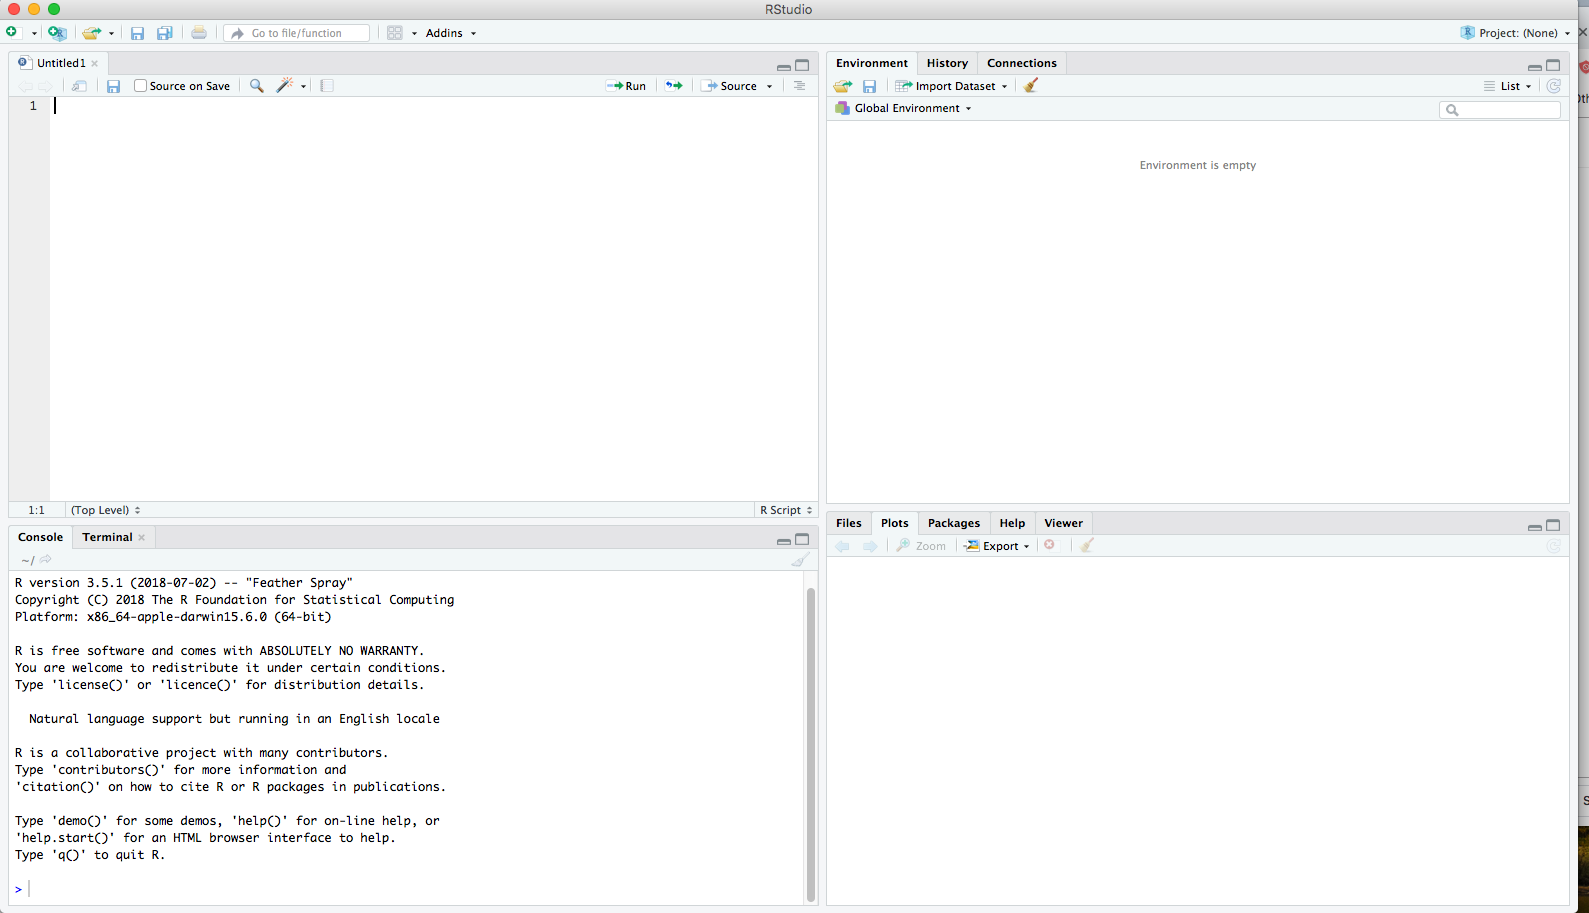
\includegraphics[width=0.7\linewidth]{./img/4-panes} \end{center}

The script editor is a great place to put code you care about. Keep
experimenting in the console, but once you have written code that works
and does what you want, put it in the script editor.

RStudio will automatically save the contents of the editor when you quit
RStudio, and will automatically load it when you re-open. Nevertheless,
it's a good idea to save your scripts regularly and to back them up.

\subsection{Running code}\label{running-code}

While you certainly can copy-paste code you'd like to run from the
editor into the console, this workflow is pretty inefficient. The key to
using the script editor effectively is to memorize one of the most
important keyboard shortcuts in RStudio:
\textbf{\texttt{Cmd/Ctrl\ +\ Enter}}. This executes the current R
expression from the script editor in the console.

For example, take the code below. If your cursor is somewhere on the
first line, pressing \texttt{Cmd/Ctrl\ +\ Enter} will run the complete
command that generates \texttt{dems}. It will also move the cursor to
the next statement (beginning with \texttt{reps}). That makes it easy to
run your complete script by repeatedly pressing
\texttt{Cmd/Ctrl\ +\ Enter}.

\begin{Shaded}
\begin{Highlighting}[]
\NormalTok{dems <-}\StringTok{ }\NormalTok{(}\DecValTok{55} \OperatorTok{+}\StringTok{ }\DecValTok{70}\NormalTok{) }\OperatorTok{*}\StringTok{ }\FloatTok{1.3}

\NormalTok{reps <-}\StringTok{ }\NormalTok{(}\DecValTok{20} \OperatorTok{-}\StringTok{ }\DecValTok{1}\NormalTok{) }\OperatorTok{/}\StringTok{ }\DecValTok{2}
\end{Highlighting}
\end{Shaded}

Instead of running expression-by-expression, you can also execute the
complete script in one step: \texttt{Cmd/Ctrl\ +\ Shift\ +\ S}. Doing
this regularly is a great way to check that you've captured all the
important parts of your code in the script.

\subsection{Comments}\label{comments}

Use \texttt{\#} signs to add comments within your code chunks, and you
are encouraged to regularly comment within your code. Anything to the
right of a \texttt{\#} is ignored by R. Each line of a comment needs to
begin with a \#.

\begin{Shaded}
\begin{Highlighting}[]
\CommentTok{# This is a comment.}
\CommentTok{# This is another line of comments.}
\end{Highlighting}
\end{Shaded}

\subsection{Diagnostics and errors}\label{diagnostics-and-errors}

The script editor will also highlight syntax errors with a red squiggly
line and a cross in the sidebar:

\begin{center}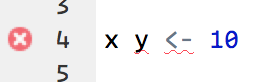
\includegraphics[width=0.7\linewidth]{img/rstudio-diagnostic} \end{center}

You can hover over the cross to see what the problem is:

\begin{center}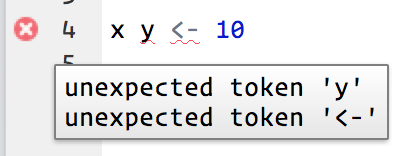
\includegraphics[width=0.7\linewidth]{img/rstudio-diagnostic-tip} \end{center}

If you try to execute the code, you'll see an error in the console.

\begin{center}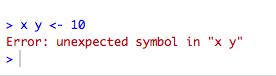
\includegraphics[width=0.7\linewidth]{img/error} \end{center}

When errors happen, your code is haulted -- meaning it's never executed.
Errors can be frustrating in R, but with practice you'll be able to
debug your code quickly.

\subsection{R Environment}\label{r-environment}

Turn your attention to the upper right pane. This pane displays your
``global environment'', and it contains the data objects you have saved
in your current session. Notice that we have the two objects created
earlier, \texttt{dems}, and \texttt{reps}, along with their values.

You can list all objects in your current environment by running:

\begin{Shaded}
\begin{Highlighting}[]
\KeywordTok{ls}\NormalTok{()}
\CommentTok{#> [1] "dems" "reps"}
\end{Highlighting}
\end{Shaded}

Sometimes we want to remove objects that we no longer need.

\begin{Shaded}
\begin{Highlighting}[]
\NormalTok{x <-}\StringTok{ }\DecValTok{5}
\KeywordTok{rm}\NormalTok{(x)}
\end{Highlighting}
\end{Shaded}

If you want to remove all objects from your current environment, you can
run:

\begin{Shaded}
\begin{Highlighting}[]
\KeywordTok{rm}\NormalTok{(}\DataTypeTok{list =} \KeywordTok{ls}\NormalTok{())}
\end{Highlighting}
\end{Shaded}

\subsubsection*{Acknowledgments}\label{acknowledgments}
\addcontentsline{toc}{subsubsection}{Acknowledgments}

This page is in part derived from the following sources:

\begin{enumerate}
\def\labelenumi{\arabic{enumi}.}
\item
  \href{https://support.rstudio.com/hc/en-us/articles/200484448}{R
  Studio Support}.
\item
  \href{https://adv-r.hadley.nz/}{Advanced R}, licensed under the
  \href{https://creativecommons.org/licenses/by-nc-sa/4.0/}{Creative
  Commons Attribution-NonCommercial-ShareAlike 4.0 International Public
  License}
\item
  \href{https://r4ds.had.co.nz}{R for Data Science} licensed under
  \href{https://creativecommons.org/licenses/by-nc-nd/3.0/us/}{Creative
  Commons Attribution-NonCommercial-NoDerivs 3.0}
\end{enumerate}

\hypertarget{r-markdown}{\section{R Markdown}\label{r-markdown}}

Throughout this course, we'll be using
\href{http://rmarkdown.rstudio.com\%3E}{R Markdown} for lecture notes
and homework assignments. R Markdown documents combine executable code,
results, and prose commentary into one document. Think of an R Markdown
files as a modern day lab notebook, where you can capture not only what
you did, but also what you were thinking.

The filename of an R Markdown document should end in \texttt{.Rmd} or
\texttt{.rmd}. They can also be converted to an output format, like PDF,
HTML, slideshows, Word files, and more.

R Markdown documents contain three important types of content:

\begin{enumerate}
\def\labelenumi{\arabic{enumi}.}
\tightlist
\item
  An (optional) YAML header surrounded by \texttt{-\/-\/-}s.
\item
  Chunks of R code surrounded by
  \texttt{\textasciigrave{}\textasciigrave{}\textasciigrave{}}.
\item
  Text mixed with simple text formatting like \texttt{\#\ heading} and
  \texttt{\_italics\_}.
\end{enumerate}

\subsection{YAML header}\label{yaml-header}

YAML stands for ``yet another markup language''. R Markdown uses it to
control many details of the output.

\begin{Shaded}
\begin{Highlighting}[]
\NormalTok{---}
\NormalTok{title: "Homework 1"}
\NormalTok{author: "Rochelle Terman"}
\NormalTok{date: "Fall 2019"}
\NormalTok{output: html_document}
\NormalTok{---}
\end{Highlighting}
\end{Shaded}

In this example, we specified the document's title, author, and date; we
also specified that we want it to eventually convert it into an HTML
document.

\subsection{Markdown}\label{markdown}

Prose in \texttt{.Rmd} files is written in Markdown, a lightweight set
of conventions for formatting plain text files. Markdown is designed to
be easy to read and easy to write. It is also very easy to learn. The
guide below shows how to use Pandoc's Markdown, a slightly extended
version of Markdown that R Markdown understands.

\begin{Shaded}
\begin{Highlighting}[]
\NormalTok{Text formatting }
\NormalTok{------------------------------------------------------------}

\NormalTok{*italic*  or _italic_}
\NormalTok{**bold**   __bold__}
\BaseNTok{`code`}
\NormalTok{superscript^2^ and subscript~2~}

\NormalTok{Headings}
\NormalTok{------------------------------------------------------------}

\FunctionTok{# 1st Level Header}

\FunctionTok{## 2nd Level Header}

\FunctionTok{### 3rd Level Header}

\NormalTok{Lists}
\NormalTok{------------------------------------------------------------}

\NormalTok{* }\FloatTok{  Bulleted list item 1}

\NormalTok{* }\FloatTok{  Item 2}

\BaseNTok{    * Item 2a}

\BaseNTok{    * Item 2b}

\NormalTok{1. }\FloatTok{ Numbered list item 1}

\NormalTok{1. }\FloatTok{ Item 2. The numbers are incremented automatically in the output.}

\NormalTok{Links and images}
\NormalTok{------------------------------------------------------------}

\OtherTok{<http://example.com>}

\OtherTok{[linked phrase](http://example.com)}

\AlertTok{![optional caption text](path/to/img.png)}

\NormalTok{Tables }
\NormalTok{------------------------------------------------------------}

\NormalTok{First Header  | Second Header}
\NormalTok{------------- | -------------}
\NormalTok{Content Cell  | Content Cell}
\NormalTok{Content Cell  | Content Cell}
\end{Highlighting}
\end{Shaded}

The best way to learn these is simply to try them out. It will take a
few days, but soon they will become second nature, and you won't need to
think about them. If you forget, you can get to a handy reference sheet
with Help \textgreater{} Markdown Quick Reference.

\subsection{Code Chunks}\label{code-chunks}

To run code inside an R Markdown document, you do it inside a ``chunk''.
Think of a chunk like a function. A chunk should be relatively
self-contained, and focused around a single task.

Chunks begin with a header which consists of
\texttt{\textasciigrave{}\textasciigrave{}\textasciigrave{}\{r,}
followed by an optional chunk name, followed by comma separated options,
followed by \texttt{\}}. Next comes your R code and the chunk end is
indicated by a final
\texttt{\textasciigrave{}\textasciigrave{}\textasciigrave{}.}

You can continue to run the code using the keyboard shortcut that we
learned earlier: \texttt{Cmd/Ctrl\ +\ Enter}. You can also run the
entire chunk by clicking the Run icon (it looks like a play button at
the top of the chunk), or by pressing
\texttt{Cmd/Ctrl\ +\ Shift\ +\ Enter}.

RStudio executes the code and displays the results inline with the code:

\begin{figure}
\centering
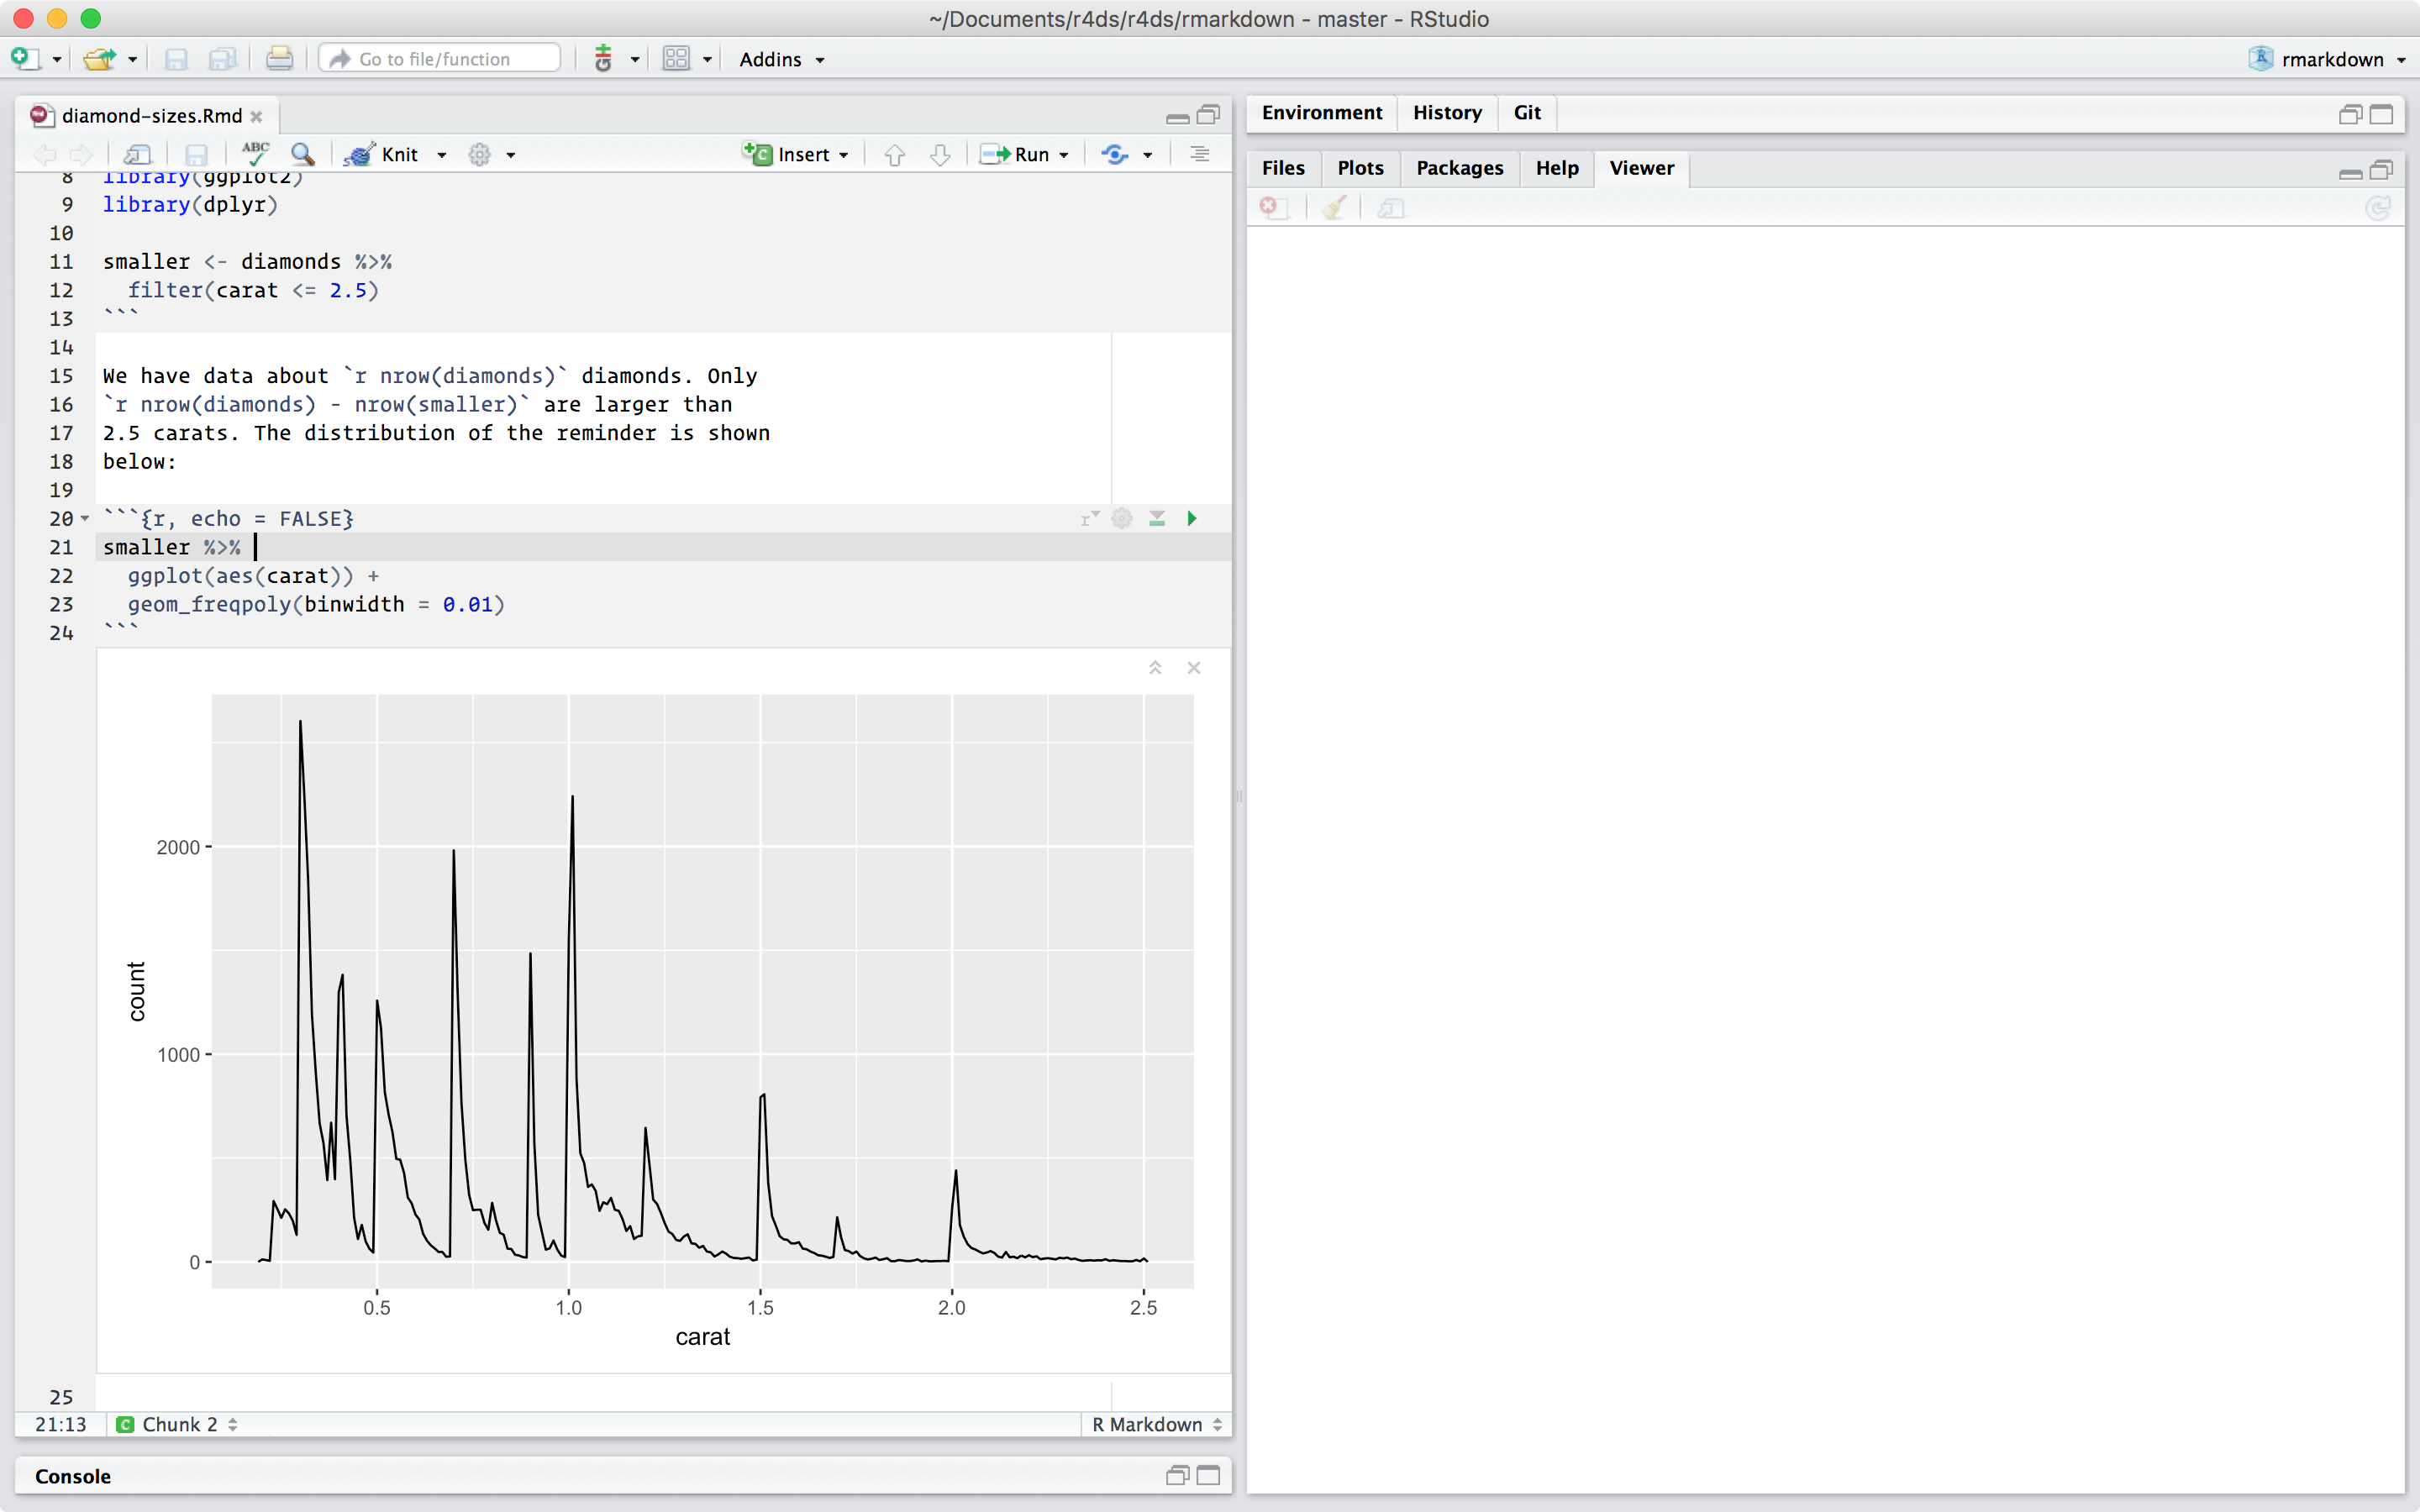
\includegraphics{img/r-markdown.png}
\caption{}
\end{figure}

\subsection{Knitting}\label{knitting}

To produce a complete report containing all text, code, and results,
click the ``Knit'' button at the top of the script editor (looks like a
ball of yarn) or press \texttt{Cmd/Ctrl\ +\ Shift\ +\ K}. This will
display the report in the viewer pane, and create a self-contained HTML
file that you can share with others. The \texttt{.html} file is written
in the same directory as your \texttt{.Rmd} file.

\subsection{Cheatsheets and Other
Resources}\label{cheatsheets-and-other-resources}

When working in RStudio, you can find an R Markdown cheatsheet by going
to Help \textgreater{} Cheatsheets \textgreater{} R Markdown Cheat
Sheet.

A helpful overview of R Markdown can also be found in
\href{https://r4ds.had.co.nz/r-markdown.html}{R for Data Science}

A deep dive into R Markdown can be found
\href{https://bookdown.org/yihui/rmarkdown/}{here}

\subsection{Challenges}\label{challenges}

\begin{enumerate}
\def\labelenumi{\arabic{enumi}.}
\item
  Create a new R Markdown document with \emph{File \textgreater{} New
  File \textgreater{} R Markdown\ldots{}} Read the instructions.
  Practice running the chunks. Verify that you can modify the code,
  re-run it, and see modified output.
\item
  Knit the document into an html file. Verify that you can modify the
  input and see the output update.
\end{enumerate}

\subsubsection*{Acknowledgments}\label{acknowledgments-1}
\addcontentsline{toc}{subsubsection}{Acknowledgments}

This page is in part derived from the following sources:

\begin{enumerate}
\def\labelenumi{\arabic{enumi}.}
\tightlist
\item
  \href{https://r4ds.had.co.nz}{R for Data Science} licensed under
  \href{https://creativecommons.org/licenses/by-nc-nd/3.0/us/}{Creative
  Commons Attribution-NonCommercial-NoDerivs 3.0}
\end{enumerate}

\hypertarget{r-packages}{\section{R Packages}\label{r-packages}}

The best part about R are its user-contributed packages (also called
``libraries''). A \emph{library} is a collection of functions (and
sometimes data) that can be used by other programers. A library's
contents are supposed to be related, but this isn't always the case as
there is no enforcement on the issue.

\subsection{Installing Packages}\label{installing-packages}

Using packages requires two steps.

First, we download the package from one of the CRAN mirrors onto our
computer. For this we use \texttt{install.packages("package-name")}. If
you have not set a preferred CRAN mirror in your \texttt{options()}, a
menu will pop up asking you to choose a location.

Let's download the package \texttt{dplyr}.

\begin{Shaded}
\begin{Highlighting}[]
\KeywordTok{install.packages}\NormalTok{(}\StringTok{"dplyr"}\NormalTok{)}
\end{Highlighting}
\end{Shaded}

If you run into errors later in the course about a function or package
not being found, run the \texttt{install.packages} function to make sure
the package is actually installed.

\textbf{Important}: Once we download the package, we never need to run
\texttt{install.packages} again (unless we get a new computer.)

\subsection{Loading Packages}\label{loading-packages}

Once we download the package, we need to load it into our session to use
it. This is required at the beginning of each R session. This step is
necessary because if we automatically loaded every package we have ever
downloaded, our computer would fry.

\begin{Shaded}
\begin{Highlighting}[]
\KeywordTok{library}\NormalTok{(dplyr)}
\end{Highlighting}
\end{Shaded}

The message tells you which functions from dplyr conflict with functions
in base R (or from other packages you might have loaded).

\subsubsection*{Challenges}\label{challenges-1}
\addcontentsline{toc}{subsubsection}{Challenges}

Let's go ahead and download some core, important packages we'll use for
the rest of the course. Download and load the following packages:

\begin{itemize}
\tightlist
\item
  tidyverse
\item
  rmarkdown
\item
  knitr
\item
  gapminder
\item
  devtools
\end{itemize}

\subsubsection*{Acknowledgments}\label{acknowledgments-2}
\addcontentsline{toc}{subsubsection}{Acknowledgments}

This page is in part derived from the following sources:

\begin{enumerate}
\def\labelenumi{\arabic{enumi}.}
\item
  \href{https://support.rstudio.com/hc/en-us/articles/200484448}{R
  Studio Support}.
\item
  \href{https://adv-r.hadley.nz/}{Advanced R}, licensed under the
  \href{https://creativecommons.org/licenses/by-nc-sa/4.0/}{Creative
  Commons Attribution-NonCommercial-ShareAlike 4.0 International Public
  License}
\item
  \href{https://r4ds.had.co.nz}{R for Data Science} licensed under
  \href{https://creativecommons.org/licenses/by-nc-nd/3.0/us/}{Creative
  Commons Attribution-NonCommercial-NoDerivs 3.0}
\end{enumerate}

\chapter{R Syntax}\label{r-syntax}

Frustration is natural when you start programming in R, because it is
such a stickler for punctuation, and even one character out of place
will cause it to complain. But while you should expect to be a little
frustrated, take comfort in that it's both typical and temporary: it
happens to everyone, and the only way to get over it is to keep trying.

\begin{quote}
To understand computations in R, two slogans are helpful: - Everything
that exists is an object. - Everything that happens is a function call.
\end{quote}

\begin{quote}
\textbf{John Chambers}
\end{quote}

\section{Variables}\label{variables}

\subsection{Arithmatic}\label{arithmatic}

In its most basic form, R can be used as a simple calculator. Consider
the following arithmetic operators:

\begin{itemize}
\tightlist
\item
  Addition: \texttt{+}
\item
  Subtraction: \texttt{-}
\item
  Multiplication: \texttt{*}
\item
  Division: \texttt{/}
\item
  Exponentiation: \texttt{\^{}}
\item
  Modulo (remainder): \texttt{\%\%}
\end{itemize}

\begin{Shaded}
\begin{Highlighting}[]
\DecValTok{1} \OperatorTok{/}\StringTok{ }\DecValTok{200} \OperatorTok{*}\StringTok{ }\DecValTok{30}
\CommentTok{#> [1] 0.15}
\NormalTok{(}\DecValTok{59} \OperatorTok{+}\StringTok{ }\DecValTok{73} \OperatorTok{+}\StringTok{ }\DecValTok{2}\NormalTok{) }\OperatorTok{/}\StringTok{ }\DecValTok{3}
\CommentTok{#> [1] 44.7}
\DecValTok{5} \OperatorTok\StringTok{ }\DecValTok{2}
\CommentTok{#> [1] 1}
\end{Highlighting}
\end{Shaded}

But when we do this, none of our results are saved for later use.

\subsection{Assigning Variables}\label{assigning-variables}

An essential part of programming is creating objects (or
variables)\footnote{Technically, objects and variables are different
  things, but we'll use the two interchangeably for now.} Variables are
names for values.

The variable is created when a value is assigned to it. We do that with
\texttt{\textless{}-}.

\begin{Shaded}
\begin{Highlighting}[]
\NormalTok{x <-}\StringTok{ }\DecValTok{3}
\end{Highlighting}
\end{Shaded}

\texttt{\textless{}-} is the called the \emph{assignment operator.} It
assigns values on the right to objects on the left, like this:

\begin{Shaded}
\begin{Highlighting}[]
\NormalTok{object_name <-}\StringTok{ }\NormalTok{value}
\end{Highlighting}
\end{Shaded}

So, after executing \texttt{x\ \textless{}-\ 3}, the value of \texttt{x}
is \texttt{3}. The arrow can be read as 3 goes into \texttt{x}.

\emph{Note:} Don't use \texttt{=} for assignments. It will work in some
contexts, but will cause confusion later.

We can use variables in calculations just as if they were values.

\begin{Shaded}
\begin{Highlighting}[]
\NormalTok{x <-}\StringTok{ }\DecValTok{3}
\NormalTok{x }\OperatorTok{+}\StringTok{ }\DecValTok{5}
\CommentTok{#> [1] 8}
\end{Highlighting}
\end{Shaded}

\subsubsection*{Inspect objects to display
values.}\label{inspect-objects-to-display-values.}
\addcontentsline{toc}{subsubsection}{Inspect objects to display values.}

In R, the contents of an object can be printed by either simply
executing the the object name.

\begin{Shaded}
\begin{Highlighting}[]
\NormalTok{x <-}\StringTok{ }\DecValTok{3}
\NormalTok{x}
\CommentTok{#> [1] 3}
\end{Highlighting}
\end{Shaded}

\subsubsection*{Whitespace makes code easier to
read.}\label{whitespace-makes-code-easier-to-read.}
\addcontentsline{toc}{subsubsection}{Whitespace makes code easier to
read.}

Notice that we surrounded \texttt{\textless{}-} with spaces. In
\texttt{R}, white space is ignored (unlike Python). But it is practice
to use spaces, because it makes code easier to read.

\begin{Shaded}
\begin{Highlighting}[]
\NormalTok{experiment<-}\StringTok{"current vs. voltage"}   \CommentTok{# this is bad}
\NormalTok{experiment <-}\StringTok{ "current vs. voltage"} \CommentTok{# this is better}
\end{Highlighting}
\end{Shaded}

\subsection{Variable Names}\label{variable-names}

Object names can only contain letters, numbers, \texttt{\_} and
\texttt{.}.

You want your object names to be descriptive. \texttt{x} is not a good
variable name (sorry!). You'll also need a convention for multiple
words. I recommend \emph{snake\_case} where you separate lowercase words
with \texttt{\_}.

\begin{Shaded}
\begin{Highlighting}[]
\NormalTok{i_use_snake_case}
\NormalTok{otherPeopleUseCamelCase}
\NormalTok{some.people.use.periods}
\NormalTok{And_aFew.People_RENOUNCEconvention}
\end{Highlighting}
\end{Shaded}

Let's make an assignment using snake\_case:

\begin{Shaded}
\begin{Highlighting}[]
\NormalTok{r_rocks <-}\StringTok{ }\DecValTok{2} \OperatorTok{^}\StringTok{ }\DecValTok{3}
\end{Highlighting}
\end{Shaded}

And let's try to inspect is:

\begin{Shaded}
\begin{Highlighting}[]
\NormalTok{r_rock}
\CommentTok{#> Error in eval(expr, envir, enclos): object 'r_rock' not found}
\NormalTok{R_rocks}
\CommentTok{#> Error in eval(expr, envir, enclos): object 'R_rocks' not found}
\end{Highlighting}
\end{Shaded}

R is case-sensitive!

\subsubsection*{Use the TAB key to
autocomplete.}\label{use-the-tab-key-to-autocomplete.}
\addcontentsline{toc}{subsubsection}{Use the TAB key to autocomplete.}

Because typos are the devil, we can use R Studio to help us type. Let's
inspect \texttt{r\_rocks} using RStudio's tab completion facility. Type
``r\_'', press TAB, add characters until you have a unique prefix, then
press return.

\begin{Shaded}
\begin{Highlighting}[]
\NormalTok{r_rocks}
\CommentTok{#> [1] 8}
\end{Highlighting}
\end{Shaded}

\subsection{Challenges - Variables}\label{challenges---variables}

\subsubsection*{Challenge 1: Making and Printing
Variables.}\label{challenge-1-making-and-printing-variables.}
\addcontentsline{toc}{subsubsection}{Challenge 1: Making and Printing
Variables.}

Make 3 variables: name (with your full name), city (where you were born)
and year (when you were born.)

\subsubsection*{Challenge 2: Swapping
Values}\label{challenge-2-swapping-values}
\addcontentsline{toc}{subsubsection}{Challenge 2: Swapping Values}

Draw a table showing the values of the variables in this program after
each statement is executed.

In simple terms, what do the last three lines of this program do?

\begin{Shaded}
\begin{Highlighting}[]
\NormalTok{lowest =}\StringTok{ }\FloatTok{1.0}
\NormalTok{highest =}\StringTok{ }\FloatTok{3.0}
\NormalTok{temp =}\StringTok{ }\NormalTok{lowest}
\NormalTok{lowest =}\StringTok{ }\NormalTok{highest}
\NormalTok{highest =}\StringTok{ }\NormalTok{temp}
\end{Highlighting}
\end{Shaded}

\subsubsection*{Challenge 3: Predicting
Values}\label{challenge-3-predicting-values}
\addcontentsline{toc}{subsubsection}{Challenge 3: Predicting Values}

What is the final value of \texttt{position} in the program below? Try
to predict the value without running the program, then check your
prediction.

\begin{Shaded}
\begin{Highlighting}[]
\NormalTok{initial =}\StringTok{ "left"}
\NormalTok{position =}\StringTok{ }\NormalTok{initial}
\NormalTok{initial =}\StringTok{ "right"}
\end{Highlighting}
\end{Shaded}

\subsubsection*{Challenge 4: Syntax}\label{challenge-4-syntax}
\addcontentsline{toc}{subsubsection}{Challenge 4: Syntax}

Why does the following code fail?

\begin{Shaded}
\begin{Highlighting}[]
\NormalTok{age }\OperatorTok{==}\StringTok{ }\DecValTok{31}
\end{Highlighting}
\end{Shaded}

and the following?

\begin{Shaded}
\begin{Highlighting}[]
\DecValTok{31}\NormalTok{ <-}\StringTok{  }\NormalTok{age}
\end{Highlighting}
\end{Shaded}

\section{Functions}\label{functions}

R has a large collection of built-in functions that helps us do things.
When we use a function, we say we're \emph{calling} a function.

\begin{Shaded}
\begin{Highlighting}[]
\KeywordTok{function_name}\NormalTok{(}\DataTypeTok{arg1 =}\NormalTok{ val1, }\DataTypeTok{arg2 =}\NormalTok{ val2, ...)}
\end{Highlighting}
\end{Shaded}

Here are some helpful built-in functions:

\begin{Shaded}
\begin{Highlighting}[]
\NormalTok{my_var <-}\StringTok{ }\KeywordTok{c}\NormalTok{(}\DecValTok{1}\NormalTok{, }\DecValTok{5}\NormalTok{, }\DecValTok{2}\NormalTok{, }\DecValTok{4}\NormalTok{, }\DecValTok{5}\NormalTok{)}

\KeywordTok{sum}\NormalTok{(my_var)}
\CommentTok{#> [1] 17}
\KeywordTok{length}\NormalTok{(my_var)}
\CommentTok{#> [1] 5}
\KeywordTok{min}\NormalTok{(my_var)}
\CommentTok{#> [1] 1}
\KeywordTok{max}\NormalTok{(my_var)}
\CommentTok{#> [1] 5}
\KeywordTok{unique}\NormalTok{(my_var)}
\CommentTok{#> [1] 1 5 2 4}
\end{Highlighting}
\end{Shaded}

\subsection{Arguments}\label{arguments}

An \emph{argument} is a value that is \emph{passed} into a function.
Every function returns a \textbf{result}.

Let's try using \texttt{seq()} which makes regular sequences of numbers
and, while we're at it, learn more helpful features of RStudio.

Type \texttt{se} and hit TAB. A popup shows you possible completions.
Specify \texttt{seq()} by typing more (a ``q) to disambiguate, or by
using ↑/↓ arrows to select. Notice the floating tooltip that pops up,
reminding you of the function's arguments and purpose.

Press TAB once more when you've selected the function you want. RStudio
will add matching opening (\texttt{(}) and closing (\texttt{)})
parentheses for you. Type the arguments \texttt{1,\ 10} and hit return.

\begin{Shaded}
\begin{Highlighting}[]
\KeywordTok{seq}\NormalTok{(}\DecValTok{1}\NormalTok{, }\DecValTok{10}\NormalTok{)}
\CommentTok{#>  [1]  1  2  3  4  5  6  7  8  9 10}
\end{Highlighting}
\end{Shaded}

How many arguments did we pass into the \texttt{seq} function?

\subsection{Store function output}\label{store-function-output}

Notice, when we called the \texttt{seq} function, that nothing changed
in our environment. That's because we didn't save our results to an
object. Let's try it again by assigning a variable.

\begin{Shaded}
\begin{Highlighting}[]
\NormalTok{y <-}\StringTok{ }\KeywordTok{seq}\NormalTok{(}\DecValTok{1}\NormalTok{, }\DecValTok{10}\NormalTok{)}
\NormalTok{y}
\CommentTok{#>  [1]  1  2  3  4  5  6  7  8  9 10}
\end{Highlighting}
\end{Shaded}

\subsection{Argument restrictions and
defaults}\label{argument-restrictions-and-defaults}

Let's use another function, called \texttt{round}:

\begin{Shaded}
\begin{Highlighting}[]
\KeywordTok{round}\NormalTok{(}\FloatTok{60.123}\NormalTok{)}
\CommentTok{#> [1] 60}
\end{Highlighting}
\end{Shaded}

\texttt{round} must be given at least one argument. And it must be given
things that can be meaningful rounded.

\begin{Shaded}
\begin{Highlighting}[]
\KeywordTok{round}\NormalTok{()}
\KeywordTok{round}\NormalTok{(}\StringTok{'a'}\NormalTok{)}
\end{Highlighting}
\end{Shaded}

Functions may have \textbf{default} values for some arguments.\{-\}

By default, \texttt{round} will round off any number to zero decimal
places. But we can specify the number of decimal places we want.

\begin{Shaded}
\begin{Highlighting}[]
\KeywordTok{round}\NormalTok{(}\FloatTok{60.123}\NormalTok{)}
\CommentTok{#> [1] 60}
\KeywordTok{round}\NormalTok{(}\FloatTok{60.123}\NormalTok{, }\DataTypeTok{digits =} \DecValTok{2}\NormalTok{)}
\CommentTok{#> [1] 60.1}
\KeywordTok{round}\NormalTok{(}\FloatTok{60.123}\NormalTok{, }\DecValTok{2}\NormalTok{)}
\CommentTok{#> [1] 60.1}
\end{Highlighting}
\end{Shaded}

\subsection{Documentation and help
files}\label{documentation-and-help-files}

How do we know what kinds of arguments to pass into a functiion? Every
built-in function comes with \_\textbf{documentation}.

\begin{itemize}
\tightlist
\item
  \texttt{?} + object opens a help page for that specific object
\item
  \texttt{??} + object searches help pages containing the name of the
  object
\end{itemize}

\begin{Shaded}
\begin{Highlighting}[]
\NormalTok{?mean}
\NormalTok{??mean}
\end{Highlighting}
\end{Shaded}

All help files are structured the same way. The section
\textbf{Arguments} tells us exactly what kind of information we can pass
into a function. The \textbf{Value} section explains what the output of
the function is. The \textbf{Examples} contain real examples of the
function in use.

\subsection{Challenges - Functions}\label{challenges---functions}

\subsubsection*{Challenge 1: What Happens
When}\label{challenge-1-what-happens-when}
\addcontentsline{toc}{subsubsection}{Challenge 1: What Happens When}

Explain in simple terms the order of operations in the following
program: when does the addition happen, when does the subtraction
happen, when is each function called, etc.

What is the final value of \texttt{radiance}?

\begin{Shaded}
\begin{Highlighting}[]
\NormalTok{radiance =}\StringTok{ }\FloatTok{1.0}
\NormalTok{radiance =}\StringTok{ }\KeywordTok{max}\NormalTok{(}\FloatTok{2.1}\NormalTok{, }\FloatTok{2.0} \OperatorTok{+}\StringTok{ }\KeywordTok{min}\NormalTok{(radiance, }\FloatTok{1.1} \OperatorTok{*}\StringTok{ }\NormalTok{radiance }\OperatorTok{-}\StringTok{ }\FloatTok{0.5}\NormalTok{))}
\end{Highlighting}
\end{Shaded}

\subsubsection*{Challenge 2: Why?}\label{challenge-2-why}
\addcontentsline{toc}{subsubsection}{Challenge 2: Why?}

Run the following code.

\begin{Shaded}
\begin{Highlighting}[]
\NormalTok{rich =}\StringTok{ "gold"}
\NormalTok{poor =}\StringTok{ "tin"}
\KeywordTok{max}\NormalTok{(rich, poor)}
\end{Highlighting}
\end{Shaded}

Using the help files for \texttt{max}, explain why it return the result
it does.

\section{Data Types}\label{data-types}

Every value in a program has a specific \textbf{type}. The R, those
types are classes ``classes'', and there are 4 of them:

\begin{itemize}
\tightlist
\item
  character (text or ``string'')
\item
  numeric (integer or decimal)
\item
  integer (just integer)
\item
  logical (TRUE or FALSE booleans)
\end{itemize}

\begin{longtable}[]{@{}ll@{}}
\toprule
Example & Type\tabularnewline
\midrule
\endhead
``a'', ``swc'' & character\tabularnewline
2, 15.5 & numeric\tabularnewline
2 (Must add a \texttt{L} at end to denote integer) &
integer\tabularnewline
\texttt{TRUE}, \texttt{FALSE} & logical\tabularnewline
\bottomrule
\end{longtable}

\subsection{What's that type?}\label{whats-that-type}

R is a dynamically typed, meaning that it ``guesses'' what class a value
is.

Use the build-in function\texttt{class()} to find out what type a value
has.

\begin{Shaded}
\begin{Highlighting}[]
\KeywordTok{class}\NormalTok{(}\DecValTok{3}\NormalTok{)}
\CommentTok{#> [1] "numeric"}
\KeywordTok{class}\NormalTok{(3L)}
\CommentTok{#> [1] "integer"}
\KeywordTok{class}\NormalTok{(}\StringTok{"Three"}\NormalTok{)}
\CommentTok{#> [1] "character"}
\KeywordTok{class}\NormalTok{(T)}
\CommentTok{#> [1] "logical"}
\end{Highlighting}
\end{Shaded}

This works on variables as well. But remember: the \emph{value} has the
type --- the \emph{variable} is just a label.

\begin{Shaded}
\begin{Highlighting}[]
\NormalTok{three <-}\StringTok{ }\DecValTok{3}
\KeywordTok{class}\NormalTok{(three)}
\CommentTok{#> [1] "numeric"}

\NormalTok{three <-}\StringTok{ "three"}
\KeywordTok{class}\NormalTok{(three)}
\CommentTok{#> [1] "character"}
\end{Highlighting}
\end{Shaded}

A value's class determines what the program can do to it.

\begin{Shaded}
\begin{Highlighting}[]
\DecValTok{3} \OperatorTok{-}\StringTok{ }\DecValTok{1}
\DecValTok{3} \OperatorTok{-}\StringTok{ "1"}
\end{Highlighting}
\end{Shaded}

\subsection{Coercion}\label{coercion}

We just learned we cannot add numbers and strings. Instead, use
\texttt{as..} + name of class as functions to convert a value to that
type.

\begin{Shaded}
\begin{Highlighting}[]
\DecValTok{3} \OperatorTok{+}\StringTok{ }\KeywordTok{as.numeric}\NormalTok{(}\StringTok{"1"}\NormalTok{)}
\end{Highlighting}
\end{Shaded}

This is called \texttt{coercion}. Here's another example:

\begin{Shaded}
\begin{Highlighting}[]
\NormalTok{my_var <-}\StringTok{ "FALSE"}
\NormalTok{my_var}
\CommentTok{#> [1] "FALSE"}
\KeywordTok{as.logical}\NormalTok{(my_var)}
\CommentTok{#> [1] FALSE}
\end{Highlighting}
\end{Shaded}

What difference did you notice?

\subsection{Other objects}\label{other-objects}

There are a few other ``odd ball'' types in R:

\subsubsection*{\texorpdfstring{\texttt{NA} are missing
values}{NA are missing values}}\label{na-are-missing-values}
\addcontentsline{toc}{subsubsection}{\texttt{NA} are missing values}

Missing values are specified with \texttt{NA}. \texttt{NA} will always
be coerced to the correct type if used inside \texttt{c()}

\begin{Shaded}
\begin{Highlighting}[]
\NormalTok{x <-}\StringTok{ }\KeywordTok{c}\NormalTok{(}\OtherTok{NA}\NormalTok{, }\DecValTok{1}\NormalTok{)}
\NormalTok{x}
\CommentTok{#> [1] NA  1}
\KeywordTok{typeof}\NormalTok{(}\OtherTok{NA}\NormalTok{)}
\CommentTok{#> [1] "logical"}
\KeywordTok{typeof}\NormalTok{(x)}
\CommentTok{#> [1] "double"}
\end{Highlighting}
\end{Shaded}

\subsubsection*{\texorpdfstring{\texttt{Inf} is
infinity.}{Inf is infinity.}}\label{inf-is-infinity.}
\addcontentsline{toc}{subsubsection}{\texttt{Inf} is infinity.}

You can have either positive or negative infinity.

\begin{Shaded}
\begin{Highlighting}[]
\DecValTok{1}\OperatorTok{/}\DecValTok{0}
\CommentTok{#> [1] Inf}
\DecValTok{1}\OperatorTok{/}\OtherTok{Inf}
\CommentTok{#> [1] 0}
\end{Highlighting}
\end{Shaded}

\subsubsection*{\texorpdfstring{\texttt{NaN} means ``Not a number''.
It's an undefined
value.}{NaN means Not a number. It's an undefined value.}}\label{nan-means-not-a-number.-its-an-undefined-value.}
\addcontentsline{toc}{subsubsection}{\texttt{NaN} means ``Not a
number''. It's an undefined value.}

\begin{Shaded}
\begin{Highlighting}[]
\DecValTok{0}\OperatorTok{/}\DecValTok{0}
\CommentTok{#> [1] NaN}
\end{Highlighting}
\end{Shaded}

\subsection{Challenges}\label{challenges-2}

\subsubsection{1: Making and Coercing
Variables}\label{making-and-coercing-variables}

\begin{enumerate}
\def\labelenumi{\arabic{enumi}.}
\tightlist
\item
  Make a variable \texttt{year} and assign it as the year you were born.
\item
  Coerce that variable to a string, and assign it to a new variable
  \texttt{year\_string}. 4 Someone in your class says they were born in
  2001. Really? Really. Find out what your age difference is, using only
  \texttt{year\_string}
\end{enumerate}

\subsubsection{2: Fix the code.}\label{fix-the-code.}

Change the following code to make the output TRUE.

\begin{Shaded}
\begin{Highlighting}[]
\NormalTok{val_}\DecValTok{1}\NormalTok{ =}\StringTok{ }\NormalTok{F}
\NormalTok{val_}\DecValTok{2}\NormalTok{ =}\StringTok{ "F"}

\KeywordTok{class}\NormalTok{(val_}\DecValTok{1}\NormalTok{) }\OperatorTok{==}\StringTok{ }\KeywordTok{class}\NormalTok{(val_}\DecValTok{2}\NormalTok{)}
\CommentTok{#> [1] FALSE}
\end{Highlighting}
\end{Shaded}

\chapter{Data Classes and Structures}\label{data-classes-and-structures}

To make the best use of the R language, you'll need a strong
understanding of basic data structures, and how to operate on them.

It is \textbf{critical} to understand, because these are the objects you
will manipulate on a day-to-day basis in R. But they are not always as
easy to work with as they sound at the outset. Dealing with object types
and conversions is one of the most common sources of frustration for
beginners.

R's base data structures can be organised by their dimensionality (1d,
2d, or nd) and whether they're homogeneous (all contents must be of the
same type) or heterogeneous (the contents can be of different types).
This gives rise to the five data types most often used in data analysis:

\begin{longtable}[]{@{}lll@{}}
\toprule
& Homogeneous & Heterogeneous\tabularnewline
\midrule
\endhead
1d & Atomic vector & List\tabularnewline
2d & Matrix & Dataframe\tabularnewline
nd & Array &\tabularnewline
\bottomrule
\end{longtable}

Each data structure has its own specifications and behavior. In the rest
of this chapter, we cover the types of data objects that exist in R and
their attributes.

\begin{enumerate}
\def\labelenumi{\arabic{enumi}.}
\tightlist
\item
  \protect\hyperlink{vectors}{Vectors}
\item
  \protect\hyperlink{lists}{Lists}
\item
  \protect\hyperlink{factors}{Factors}
\item
  \protect\hyperlink{matrices}{Matrices}
\item
  \protect\hyperlink{dataframes}{Dataframes}
\end{enumerate}

\hypertarget{vectors}{\section{Vectors}\label{vectors}}

Let's start with one-dimensional (1d) objects. There are two kinds:

\begin{enumerate}
\def\labelenumi{\arabic{enumi}.}
\tightlist
\item
  \textbf{Atomic vectors} - also called, simply, \textbf{vectors}.
\item
  \textbf{Lists}: Lists are distinct from atomic vectors because lists
  can contain other lists.
\end{enumerate}

We'll discuss \textbf{atomic vectors} first.

\subsection{Creating Vectors}\label{creating-vectors}

Vectors are 1-dimensional chain of values. We call each value an
\emph{element} of a vector.

Atomic vectors are usually created with \texttt{c()}, which is short for
`combine':

\begin{Shaded}
\begin{Highlighting}[]
\NormalTok{x <-}\StringTok{ }\KeywordTok{c}\NormalTok{(}\DecValTok{1}\NormalTok{, }\DecValTok{2}\NormalTok{, }\DecValTok{3}\NormalTok{)}
\NormalTok{x}
\CommentTok{#> [1] 1 2 3}
\KeywordTok{length}\NormalTok{(x)}
\CommentTok{#> [1] 3}
\end{Highlighting}
\end{Shaded}

We can also add elements to the end of a vector by passing the original
vector into the \texttt{c} function, like so:

\begin{Shaded}
\begin{Highlighting}[]
\NormalTok{z <-}\StringTok{ }\KeywordTok{c}\NormalTok{(}\StringTok{"Beyonce"}\NormalTok{, }\StringTok{"Kelly"}\NormalTok{, }\StringTok{"Michelle"}\NormalTok{, }\StringTok{"LeToya"}\NormalTok{)}
\NormalTok{z <-}\StringTok{ }\KeywordTok{c}\NormalTok{(z, }\StringTok{"Farrah"}\NormalTok{)}
\NormalTok{z}
\CommentTok{#> [1] "Beyonce"  "Kelly"    "Michelle" "LeToya"   "Farrah"}
\end{Highlighting}
\end{Shaded}

Notice that vectors are always flat, even if you nest \texttt{c()}'s:

\begin{Shaded}
\begin{Highlighting}[]
\CommentTok{# these are equivalent}
\KeywordTok{c}\NormalTok{(}\DecValTok{1}\NormalTok{, }\KeywordTok{c}\NormalTok{(}\DecValTok{2}\NormalTok{, }\KeywordTok{c}\NormalTok{(}\DecValTok{3}\NormalTok{, }\DecValTok{4}\NormalTok{)))}
\CommentTok{#> [1] 1 2 3 4}
\KeywordTok{c}\NormalTok{(}\DecValTok{1}\NormalTok{, }\DecValTok{2}\NormalTok{, }\DecValTok{3}\NormalTok{, }\DecValTok{4}\NormalTok{)}
\CommentTok{#> [1] 1 2 3 4}
\end{Highlighting}
\end{Shaded}

\subsection{Naming a vector}\label{naming-a-vector}

We can also attach names to our vector. This helps us understand what
each element refers to.

You can give a name to the elements of a vector with the
\texttt{names()} function. Have a look at this example:

\begin{Shaded}
\begin{Highlighting}[]
\NormalTok{days_month <-}\StringTok{ }\KeywordTok{c}\NormalTok{(}\DecValTok{31}\NormalTok{, }\DecValTok{28}\NormalTok{, }\DecValTok{31}\NormalTok{, }\DecValTok{30}\NormalTok{, }\DecValTok{31}\NormalTok{, }\DecValTok{30}\NormalTok{, }\DecValTok{31}\NormalTok{, }\DecValTok{31}\NormalTok{, }\DecValTok{30}\NormalTok{, }\DecValTok{31}\NormalTok{, }\DecValTok{30}\NormalTok{, }\DecValTok{31}\NormalTok{)}
\KeywordTok{names}\NormalTok{(days_month) <-}\StringTok{ }\KeywordTok{c}\NormalTok{(}\StringTok{"Jan"}\NormalTok{, }\StringTok{"Feb"}\NormalTok{, }\StringTok{"Mar"}\NormalTok{, }\StringTok{"Apr"}\NormalTok{, }\StringTok{"May"}\NormalTok{, }\StringTok{"Jun"}\NormalTok{, }\StringTok{"Jul"}\NormalTok{, }\StringTok{"Aug"}\NormalTok{, }\StringTok{"Sep"}\NormalTok{, }\StringTok{"Oct"}\NormalTok{, }\StringTok{"Nov"}\NormalTok{, }\StringTok{"Dec"}\NormalTok{)}

\NormalTok{days_month}
\CommentTok{#> Jan Feb Mar Apr May Jun Jul Aug Sep Oct Nov Dec }
\CommentTok{#>  31  28  31  30  31  30  31  31  30  31  30  31}
\end{Highlighting}
\end{Shaded}

You can name a vector when you create it:

\begin{Shaded}
\begin{Highlighting}[]
\NormalTok{some_vector <-}\StringTok{ }\KeywordTok{c}\NormalTok{(}\DataTypeTok{name =} \StringTok{"Rochelle Terman"}\NormalTok{, }\DataTypeTok{profession =} \StringTok{"Professor Extraordinaire"}\NormalTok{)}
\NormalTok{some_vector}
\CommentTok{#>                       name                 profession }
\CommentTok{#>          "Rochelle Terman" "Professor Extraordinaire"}
\end{Highlighting}
\end{Shaded}

Notice that in the first case, we surrounded each name with quotation
marks. But we don't have to do this when creating a named vector.

Names don't have to be unique, and not all value has to have a name
associated. However, names are most useful for subsetting, described in
the next chapter. When subsetting, it is most useful when the names are
unique.

\subsection{Calculations on Vectors}\label{calculations-on-vectors}

One of the most powerful things about vectors is that we can perform
arithmetic calculations on them.

For example, we can sum up all the values in a numerical vector using
\textbf{sum}:

\begin{Shaded}
\begin{Highlighting}[]
\NormalTok{a <-}\StringTok{ }\KeywordTok{c}\NormalTok{(}\DecValTok{1}\NormalTok{, }\OperatorTok{-}\DecValTok{2}\NormalTok{, }\DecValTok{3}\NormalTok{)}
\KeywordTok{sum}\NormalTok{(a)}
\CommentTok{#> [1] 2}
\end{Highlighting}
\end{Shaded}

We can also sum two vectors. It is important to know that if you
\textbf{sum} two vectors in R, it takes the element-wise sum. For
example, the following three statements are completely equivalent:

\begin{Shaded}
\begin{Highlighting}[]
\KeywordTok{c}\NormalTok{(}\DecValTok{1}\NormalTok{, }\DecValTok{2}\NormalTok{, }\DecValTok{3}\NormalTok{) }\OperatorTok{+}\StringTok{ }\KeywordTok{c}\NormalTok{(}\DecValTok{4}\NormalTok{, }\DecValTok{5}\NormalTok{, }\DecValTok{6}\NormalTok{)}
\KeywordTok{c}\NormalTok{(}\DecValTok{1} \OperatorTok{+}\StringTok{ }\DecValTok{4}\NormalTok{, }\DecValTok{2} \OperatorTok{+}\StringTok{ }\DecValTok{5}\NormalTok{, }\DecValTok{3} \OperatorTok{+}\StringTok{ }\DecValTok{6}\NormalTok{)}
\KeywordTok{c}\NormalTok{(}\DecValTok{5}\NormalTok{, }\DecValTok{7}\NormalTok{, }\DecValTok{9}\NormalTok{)}
\end{Highlighting}
\end{Shaded}

\subsection{Types of Vectors}\label{types-of-vectors}

So there are there are four common types of vectors, depending on the
class: * \texttt{logical} * \texttt{integer} * \texttt{numeric} (same as
\texttt{double}) * \texttt{character}.

\subsubsection*{Logical vectors}\label{logical-vectors}
\addcontentsline{toc}{subsubsection}{Logical vectors}

Logical vectors take on one of three possible values:

\begin{enumerate}
\def\labelenumi{\arabic{enumi}.}
\tightlist
\item
  \texttt{TRUE}
\item
  \texttt{FALSE}
\item
  \texttt{NA} (missing value)
\end{enumerate}

\begin{Shaded}
\begin{Highlighting}[]
\KeywordTok{c}\NormalTok{(}\OtherTok{TRUE}\NormalTok{, }\OtherTok{TRUE}\NormalTok{, }\OtherTok{FALSE}\NormalTok{, }\OtherTok{NA}\NormalTok{)}
\CommentTok{#> [1]  TRUE  TRUE FALSE    NA}
\end{Highlighting}
\end{Shaded}

\subsubsection*{Numerical vectors}\label{numerical-vectors}
\addcontentsline{toc}{subsubsection}{Numerical vectors}

Numeric vectors contain numbers. They can be stored as \emph{integers}
(whole numbers) or \emph{doubles} (numbers with decimal points). In
practice, you rarely need to concern yourself with this difference, but
just know that they are different but related things.

\begin{Shaded}
\begin{Highlighting}[]
\KeywordTok{c}\NormalTok{(}\DecValTok{1}\NormalTok{, }\DecValTok{2}\NormalTok{, }\DecValTok{335}\NormalTok{)}
\CommentTok{#> [1]   1   2 335}
\KeywordTok{c}\NormalTok{(}\FloatTok{4.2}\NormalTok{, }\DecValTok{4}\NormalTok{, }\DecValTok{6}\NormalTok{, }\FloatTok{53.2}\NormalTok{)}
\CommentTok{#> [1]  4.2  4.0  6.0 53.2}
\end{Highlighting}
\end{Shaded}

\subsubsection*{Character vectors}\label{character-vectors}
\addcontentsline{toc}{subsubsection}{Character vectors}

Character vectors contain character (or `string') values. Note that each
value has to be surrounded by quotation marks \emph{before} the comma.

\begin{Shaded}
\begin{Highlighting}[]
\KeywordTok{c}\NormalTok{(}\StringTok{"Beyonce"}\NormalTok{, }\StringTok{"Kelly"}\NormalTok{, }\StringTok{"Michelle"}\NormalTok{, }\StringTok{"LeToya"}\NormalTok{)}
\CommentTok{#> [1] "Beyonce"  "Kelly"    "Michelle" "LeToya"}
\end{Highlighting}
\end{Shaded}

\subsection{Coercion}\label{coercion-1}

We can change or convert a vector's type using \texttt{as....}.

\begin{Shaded}
\begin{Highlighting}[]
\NormalTok{num_var <-}\StringTok{ }\KeywordTok{c}\NormalTok{(}\DecValTok{1}\NormalTok{, }\FloatTok{2.5}\NormalTok{, }\FloatTok{4.5}\NormalTok{)}
\KeywordTok{class}\NormalTok{(num_var)}
\CommentTok{#> [1] "numeric"}
\KeywordTok{as.character}\NormalTok{(num_var)}
\CommentTok{#> [1] "1"   "2.5" "4.5"}
\end{Highlighting}
\end{Shaded}

Remember that elements of a vector must be the same type. So when you
attempt to combine different types they will be \textbf{coerced} to the
most ``flexible'' type.

For example, combining a character and an integer yields a character:

\begin{Shaded}
\begin{Highlighting}[]
\KeywordTok{c}\NormalTok{(}\StringTok{"a"}\NormalTok{, }\DecValTok{1}\NormalTok{)}
\CommentTok{#> [1] "a" "1"}
\end{Highlighting}
\end{Shaded}

Guess what the following do without running them first:

\begin{Shaded}
\begin{Highlighting}[]
\KeywordTok{c}\NormalTok{(}\FloatTok{1.7}\NormalTok{, }\StringTok{"a"}\NormalTok{) }
\KeywordTok{c}\NormalTok{(}\OtherTok{TRUE}\NormalTok{, }\DecValTok{2}\NormalTok{) }
\KeywordTok{c}\NormalTok{(}\StringTok{"a"}\NormalTok{, }\OtherTok{TRUE}\NormalTok{) }
\end{Highlighting}
\end{Shaded}

\subsubsection*{TRUE == 1 and FALSE == 0.}\label{true-1-and-false-0.}
\addcontentsline{toc}{subsubsection}{TRUE == 1 and FALSE == 0.}

Notice that when a logical vector is coerced to an integer or double,
\texttt{TRUE} becomes 1 and \texttt{FALSE} becomes 0. This is very
useful in conjunction with \texttt{sum()} and \texttt{mean()}

\begin{Shaded}
\begin{Highlighting}[]
\NormalTok{x <-}\StringTok{ }\KeywordTok{c}\NormalTok{(}\OtherTok{FALSE}\NormalTok{, }\OtherTok{FALSE}\NormalTok{, }\OtherTok{TRUE}\NormalTok{)}
\KeywordTok{as.numeric}\NormalTok{(x)}
\CommentTok{#> [1] 0 0 1}

\CommentTok{# Total number of TRUEs}
\KeywordTok{sum}\NormalTok{(x)}
\CommentTok{#> [1] 1}

\CommentTok{# Proportion that are TRUE}
\KeywordTok{mean}\NormalTok{(x)}
\CommentTok{#> [1] 0.333}
\end{Highlighting}
\end{Shaded}

\subsubsection*{Coercion often happens
automatically.}\label{coercion-often-happens-automatically.}
\addcontentsline{toc}{subsubsection}{Coercion often happens
automatically.}

This is called \emph{implicit coercion}. Most mathematical functions
(\texttt{+}, \texttt{log}, \texttt{abs}, etc.) will coerce to a double
or integer, and most logical operations (\texttt{\&},
\texttt{\textbar{}}, \texttt{any}, etc) will coerce to a logical. You
will usually get a warning message if the coercion might lose
information.

\begin{Shaded}
\begin{Highlighting}[]
\DecValTok{1} \OperatorTok{<}\StringTok{ "2"}
\CommentTok{#> [1] TRUE}
\StringTok{"1"} \OperatorTok{>}\StringTok{ }\DecValTok{2}
\CommentTok{#> [1] FALSE}
\end{Highlighting}
\end{Shaded}

Sometimes coercions, especially nonsensical ones, won't work.

\begin{Shaded}
\begin{Highlighting}[]
\NormalTok{x <-}\StringTok{ }\KeywordTok{c}\NormalTok{(}\StringTok{"a"}\NormalTok{, }\StringTok{"b"}\NormalTok{, }\StringTok{"c"}\NormalTok{)}
\KeywordTok{as.numeric}\NormalTok{(x)}
\CommentTok{#> Warning: NAs introduced by coercion}
\CommentTok{#> [1] NA NA NA}
\KeywordTok{as.logical}\NormalTok{(x)}
\CommentTok{#> [1] NA NA NA}
\end{Highlighting}
\end{Shaded}

\subsection{Challenges}\label{challenges-3}

\subsubsection{1: Create and examine your
vector}\label{create-and-examine-your-vector}

Create a character vector called \texttt{fruit} that contain 4 of your
favorite fruits. Then evaluate its structure using the commands below.

\begin{Shaded}
\begin{Highlighting}[]

\CommentTok{# First create your fruit vector }
\CommentTok{# YOUR CODE HERE}


\CommentTok{# Examine your vector}
\KeywordTok{length}\NormalTok{(fruit)}
\KeywordTok{class}\NormalTok{(fruit)}
\KeywordTok{str}\NormalTok{(fruit)}
\end{Highlighting}
\end{Shaded}

\subsubsection{2: Coercion}\label{coercion-2}

\begin{Shaded}
\begin{Highlighting}[]

\CommentTok{# 1. Create a vector of a sequence of numbers between 1 to 10.}

\CommentTok{# 2. Coerce that vector into a character vector}

\CommentTok{# 3. Add the element "11" to the end of the vector}

\CommentTok{# 4. Coerce it back to a numeric vector.}
\end{Highlighting}
\end{Shaded}

\subsubsection{3: Calculations on
Vectors}\label{calculations-on-vectors-1}

\hypertarget{lists}{\section{Lists}\label{lists}}

Lists are different from vectors because their elements can be of
\textbf{any type}. Lists are sometimes called recursive vectors, because
a list can contain other lists. This makes them fundamentally different
from vectors.

\subsection{Creating Lists}\label{creating-lists}

You construct lists by using \texttt{list()} instead of \texttt{c()}:

\begin{Shaded}
\begin{Highlighting}[]
\NormalTok{x <-}\StringTok{ }\KeywordTok{list}\NormalTok{(}\DecValTok{1}\NormalTok{, }\StringTok{"a"}\NormalTok{, }\OtherTok{TRUE}\NormalTok{, }\KeywordTok{c}\NormalTok{(}\DecValTok{4}\NormalTok{, }\DecValTok{5}\NormalTok{, }\DecValTok{6}\NormalTok{))}
\NormalTok{x}
\CommentTok{#> [[1]]}
\CommentTok{#> [1] 1}
\CommentTok{#> }
\CommentTok{#> [[2]]}
\CommentTok{#> [1] "a"}
\CommentTok{#> }
\CommentTok{#> [[3]]}
\CommentTok{#> [1] TRUE}
\CommentTok{#> }
\CommentTok{#> [[4]]}
\CommentTok{#> [1] 4 5 6}
\end{Highlighting}
\end{Shaded}

\subsection{Naming lists}\label{naming-lists}

As with vectors, we can attach names to each element on our list:

\begin{Shaded}
\begin{Highlighting}[]
\NormalTok{my_list <-}\StringTok{ }\KeywordTok{list}\NormalTok{(}\DataTypeTok{name1 =}\NormalTok{ elem1, }
                \DataTypeTok{name2 =}\NormalTok{ elem2)}
\end{Highlighting}
\end{Shaded}

This creates a list with components that are named \texttt{name1},
\texttt{name2\textasciigrave{}\textasciigrave{},\ and\ so\ on.\ If\ you\ want\ to\ name\ your\ lists\ after\ you\textquotesingle{}ve\ created\ them,\ you\ can\ use\ the}names()`
function as you did with vectors. The following commands are fully
equivalent to the assignment above:

\begin{Shaded}
\begin{Highlighting}[]
\NormalTok{my_list <-}\StringTok{ }\KeywordTok{list}\NormalTok{(elem1, elem2)}
\KeywordTok{names}\NormalTok{(my_list) <-}\StringTok{ }\KeywordTok{c}\NormalTok{(}\StringTok{"name1"}\NormalTok{, }\StringTok{"name2"}\NormalTok{)}
\end{Highlighting}
\end{Shaded}

\subsection{List Structure}\label{list-structure}

A very useful tool for working with lists is \texttt{str()} because it
focusses on the structure, not the contents.

\begin{Shaded}
\begin{Highlighting}[]
\NormalTok{x <-}\StringTok{ }\KeywordTok{list}\NormalTok{(}\DataTypeTok{a =} \KeywordTok{c}\NormalTok{(}\DecValTok{1}\NormalTok{, }\DecValTok{2}\NormalTok{, }\DecValTok{3}\NormalTok{),}
          \DataTypeTok{b =} \KeywordTok{c}\NormalTok{(}\StringTok{"Hello"}\NormalTok{, }\StringTok{"there"}\NormalTok{),}
          \DataTypeTok{c =} \DecValTok{1}\OperatorTok{:}\DecValTok{10}\NormalTok{)}
\KeywordTok{str}\NormalTok{(x)}
\CommentTok{#> List of 3}
\CommentTok{#>  $ a: num [1:3] 1 2 3}
\CommentTok{#>  $ b: chr [1:2] "Hello" "there"}
\CommentTok{#>  $ c: int [1:10] 1 2 3 4 5 6 7 8 9 10}
\end{Highlighting}
\end{Shaded}

A list does not print to the console like a vector. Instead, each
element of the list starts on a new line.

\begin{Shaded}
\begin{Highlighting}[]
\NormalTok{x.vec <-}\StringTok{ }\KeywordTok{c}\NormalTok{(}\DecValTok{1}\NormalTok{,}\DecValTok{2}\NormalTok{,}\DecValTok{3}\NormalTok{)}
\NormalTok{x.list <-}\StringTok{ }\KeywordTok{list}\NormalTok{(}\DecValTok{1}\NormalTok{,}\DecValTok{2}\NormalTok{,}\DecValTok{3}\NormalTok{)}
\NormalTok{x.vec}
\CommentTok{#> [1] 1 2 3}
\NormalTok{x.list}
\CommentTok{#> [[1]]}
\CommentTok{#> [1] 1}
\CommentTok{#> }
\CommentTok{#> [[2]]}
\CommentTok{#> [1] 2}
\CommentTok{#> }
\CommentTok{#> [[3]]}
\CommentTok{#> [1] 3}
\end{Highlighting}
\end{Shaded}

Lists are used to build up many of the more complicated data structures
in R. For example, both data frames and linear models objects (as
produced by \texttt{lm()}) are lists:

\begin{Shaded}
\begin{Highlighting}[]
\KeywordTok{head}\NormalTok{(mtcars)}
\CommentTok{#>                    mpg cyl disp  hp drat   wt qsec vs am gear carb}
\CommentTok{#> Mazda RX4         21.0   6  160 110 3.90 2.62 16.5  0  1    4    4}
\CommentTok{#> Mazda RX4 Wag     21.0   6  160 110 3.90 2.88 17.0  0  1    4    4}
\CommentTok{#> Datsun 710        22.8   4  108  93 3.85 2.32 18.6  1  1    4    1}
\CommentTok{#> Hornet 4 Drive    21.4   6  258 110 3.08 3.21 19.4  1  0    3    1}
\CommentTok{#> Hornet Sportabout 18.7   8  360 175 3.15 3.44 17.0  0  0    3    2}
\CommentTok{#> Valiant           18.1   6  225 105 2.76 3.46 20.2  1  0    3    1}
\KeywordTok{is.list}\NormalTok{(mtcars)}
\CommentTok{#> [1] TRUE}
\NormalTok{mod <-}\StringTok{ }\KeywordTok{lm}\NormalTok{(mpg }\OperatorTok{~}\StringTok{ }\NormalTok{wt, }\DataTypeTok{data =}\NormalTok{ mtcars)}
\KeywordTok{is.list}\NormalTok{(mod)}
\CommentTok{#> [1] TRUE}
\end{Highlighting}
\end{Shaded}

You could say that a list is some kind super data type: you can store
practically any piece of information in it!

For this reason, lists are extremely useful inside functions. You can
``staple'' together lots of different kinds of results into a single
object that a function can return.

\begin{Shaded}
\begin{Highlighting}[]
\NormalTok{mod <-}\StringTok{ }\KeywordTok{lm}\NormalTok{(mpg }\OperatorTok{~}\StringTok{ }\NormalTok{wt, }\DataTypeTok{data =}\NormalTok{ mtcars)}
\KeywordTok{str}\NormalTok{(mod)}
\CommentTok{#> List of 12}
\CommentTok{#>  $ coefficients : Named num [1:2] 37.29 -5.34}
\CommentTok{#>   ..- attr(*, "names")= chr [1:2] "(Intercept)" "wt"}
\CommentTok{#>  $ residuals    : Named num [1:32] -2.28 -0.92 -2.09 1.3 -0.2 ...}
\CommentTok{#>   ..- attr(*, "names")= chr [1:32] "Mazda RX4" "Mazda RX4 Wag" "Datsun 710" "Hornet 4 Drive" ...}
\CommentTok{#>  $ effects      : Named num [1:32] -113.65 -29.116 -1.661 1.631 0.111 ...}
\CommentTok{#>   ..- attr(*, "names")= chr [1:32] "(Intercept)" "wt" "" "" ...}
\CommentTok{#>  $ rank         : int 2}
\CommentTok{#>  $ fitted.values: Named num [1:32] 23.3 21.9 24.9 20.1 18.9 ...}
\CommentTok{#>   ..- attr(*, "names")= chr [1:32] "Mazda RX4" "Mazda RX4 Wag" "Datsun 710" "Hornet 4 Drive" ...}
\CommentTok{#>  $ assign       : int [1:2] 0 1}
\CommentTok{#>  $ qr           :List of 5}
\CommentTok{#>   ..$ qr   : num [1:32, 1:2] -5.657 0.177 0.177 0.177 0.177 ...}
\CommentTok{#>   .. ..- attr(*, "dimnames")=List of 2}
\CommentTok{#>   .. .. ..$ : chr [1:32] "Mazda RX4" "Mazda RX4 Wag" "Datsun 710" "Hornet 4 Drive" ...}
\CommentTok{#>   .. .. ..$ : chr [1:2] "(Intercept)" "wt"}
\CommentTok{#>   .. ..- attr(*, "assign")= int [1:2] 0 1}
\CommentTok{#>   ..$ qraux: num [1:2] 1.18 1.05}
\CommentTok{#>   ..$ pivot: int [1:2] 1 2}
\CommentTok{#>   ..$ tol  : num 1e-07}
\CommentTok{#>   ..$ rank : int 2}
\CommentTok{#>   ..- attr(*, "class")= chr "qr"}
\CommentTok{#>  $ df.residual  : int 30}
\CommentTok{#>  $ xlevels      : Named list()}
\CommentTok{#>  $ call         : language lm(formula = mpg ~ wt, data = mtcars)}
\CommentTok{#>  $ terms        :Classes 'terms', 'formula'  language mpg ~ wt}
\CommentTok{#>   .. ..- attr(*, "variables")= language list(mpg, wt)}
\CommentTok{#>   .. ..- attr(*, "factors")= int [1:2, 1] 0 1}
\CommentTok{#>   .. .. ..- attr(*, "dimnames")=List of 2}
\CommentTok{#>   .. .. .. ..$ : chr [1:2] "mpg" "wt"}
\CommentTok{#>   .. .. .. ..$ : chr "wt"}
\CommentTok{#>   .. ..- attr(*, "term.labels")= chr "wt"}
\CommentTok{#>   .. ..- attr(*, "order")= int 1}
\CommentTok{#>   .. ..- attr(*, "intercept")= int 1}
\CommentTok{#>   .. ..- attr(*, "response")= int 1}
\CommentTok{#>   .. ..- attr(*, ".Environment")=<environment: R_GlobalEnv> }
\CommentTok{#>   .. ..- attr(*, "predvars")= language list(mpg, wt)}
\CommentTok{#>   .. ..- attr(*, "dataClasses")= Named chr [1:2] "numeric" "numeric"}
\CommentTok{#>   .. .. ..- attr(*, "names")= chr [1:2] "mpg" "wt"}
\CommentTok{#>  $ model        :'data.frame':   32 obs. of  2 variables:}
\CommentTok{#>   ..$ mpg: num [1:32] 21 21 22.8 21.4 18.7 18.1 14.3 24.4 22.8 19.2 ...}
\CommentTok{#>   ..$ wt : num [1:32] 2.62 2.88 2.32 3.21 3.44 ...}
\CommentTok{#>   ..- attr(*, "terms")=Classes 'terms', 'formula'  language mpg ~ wt}
\CommentTok{#>   .. .. ..- attr(*, "variables")= language list(mpg, wt)}
\CommentTok{#>   .. .. ..- attr(*, "factors")= int [1:2, 1] 0 1}
\CommentTok{#>   .. .. .. ..- attr(*, "dimnames")=List of 2}
\CommentTok{#>   .. .. .. .. ..$ : chr [1:2] "mpg" "wt"}
\CommentTok{#>   .. .. .. .. ..$ : chr "wt"}
\CommentTok{#>   .. .. ..- attr(*, "term.labels")= chr "wt"}
\CommentTok{#>   .. .. ..- attr(*, "order")= int 1}
\CommentTok{#>   .. .. ..- attr(*, "intercept")= int 1}
\CommentTok{#>   .. .. ..- attr(*, "response")= int 1}
\CommentTok{#>   .. .. ..- attr(*, ".Environment")=<environment: R_GlobalEnv> }
\CommentTok{#>   .. .. ..- attr(*, "predvars")= language list(mpg, wt)}
\CommentTok{#>   .. .. ..- attr(*, "dataClasses")= Named chr [1:2] "numeric" "numeric"}
\CommentTok{#>   .. .. .. ..- attr(*, "names")= chr [1:2] "mpg" "wt"}
\CommentTok{#>  - attr(*, "class")= chr "lm"}
\end{Highlighting}
\end{Shaded}

\subsection{Challenges}\label{challenges-4}

\begin{enumerate}
\def\labelenumi{\arabic{enumi}.}
\item
  What are the four basic types of atomic vector? How does a list differ
  from an atomic vector?
\item
  Why is \texttt{1\ ==\ "1"} true? Why is
  \texttt{-1\ \textless{}\ FALSE} true? Why is
  \texttt{"one"\ \textless{}\ 2} false?
\item
  Create three vectors and then combine them into a list. Assign them
  names.
\item
  If \texttt{x} is a list, what is the class of \texttt{x{[}1{]}}? How
  about \texttt{x{[}{[}1{]}{]}}?
\end{enumerate}

\hypertarget{factors}{\section{Factors}\label{factors}}

Factors are special vectors that represent \emph{categorical} data:
variables that have a fixed and known set of possible values. Think:
Democrat, Republican, Independent; Male, Female, Other; etc.

It is important that R knows whether it is dealing with a continuous or
a categorical variable, as the statistical models you will develop in
the future treat both types differently.

Historically, factors were much easier to work with than characters. As
a result, many of the functions in base R automatically convert
characters to factors. This means that factors often crop up in places
where they're not actually helpful.

\subsection{Creating Factors}\label{creating-factors}

To create factors in R, you make use of the function \texttt{factor()}.
First thing that you have to do is create a vector that contains all the
observations that belong to a limited number of categories. For example,
\texttt{party\_vector} contains the partyID of 5 different individuals:

\begin{Shaded}
\begin{Highlighting}[]
\NormalTok{party_vector <-}\StringTok{ }\KeywordTok{c}\NormalTok{(}\StringTok{"Rep"}\NormalTok{, }\StringTok{"Rep"}\NormalTok{, }\StringTok{"Dem"}\NormalTok{, }\StringTok{"Rep"}\NormalTok{, }\StringTok{"Dem"}\NormalTok{)}
\end{Highlighting}
\end{Shaded}

It is clear that there are two categories, or in R-terms \textbf{factor
levels}, at work here: \texttt{Dem} and \texttt{Rep}.

The function \texttt{factor()} will encode the vector as a factor:

\begin{Shaded}
\begin{Highlighting}[]
\NormalTok{party_factor <-}\StringTok{ }\KeywordTok{factor}\NormalTok{(party_vector)}
\NormalTok{party_vector}
\CommentTok{#> [1] "Rep" "Rep" "Dem" "Rep" "Dem"}
\NormalTok{party_factor}
\CommentTok{#> [1] Rep Rep Dem Rep Dem}
\CommentTok{#> Levels: Dem Rep}
\end{Highlighting}
\end{Shaded}

\subsection{Summarizing a Factor}\label{summarizing-a-factor}

One of your favorite functions in R will be \texttt{summary()}. This
will give you a quick overview of the contents of a variable. Let's
compare using \texttt{summary()} on the character vector, and on the
factor:

\begin{Shaded}
\begin{Highlighting}[]
\KeywordTok{summary}\NormalTok{(party_vector)}
\KeywordTok{summary}\NormalTok{(party_factor)}
\end{Highlighting}
\end{Shaded}

\subsection{Changing Factor Levels}\label{changing-factor-levels}

When you create the factor, the factor levels are set to specific
values. We can access those values with the \texttt{levels()} function.

\begin{Shaded}
\begin{Highlighting}[]
\KeywordTok{levels}\NormalTok{(party_factor)}
\CommentTok{#> [1] "Dem" "Rep"}
\end{Highlighting}
\end{Shaded}

Any values \emph{not} in the set of levels will be silently converted to
\texttt{NA}. Let's say we want to add an Independent to our sample:

\begin{Shaded}
\begin{Highlighting}[]
\NormalTok{party_factor[}\DecValTok{5}\NormalTok{] <-}\StringTok{ "Ind"}
\CommentTok{#> Warning in `[<-.factor`(`*tmp*`, 5, value = "Ind"): invalid factor level,}
\CommentTok{#> NA generated}
\NormalTok{party_factor}
\CommentTok{#> [1] Rep  Rep  Dem  Rep  <NA>}
\CommentTok{#> Levels: Dem Rep}
\end{Highlighting}
\end{Shaded}

We first need to add ``Ind'' to our factor levels. This will allow us to
add Independents to our sample:

\begin{Shaded}
\begin{Highlighting}[]
\KeywordTok{levels}\NormalTok{(party_factor)}
\CommentTok{#> [1] "Dem" "Rep"}
\KeywordTok{levels}\NormalTok{(party_factor) <-}\StringTok{ }\KeywordTok{c}\NormalTok{(}\StringTok{"Dem"}\NormalTok{, }\StringTok{"Rep"}\NormalTok{, }\StringTok{"Ind"}\NormalTok{)}

\NormalTok{party_factor[}\DecValTok{5}\NormalTok{] <-}\StringTok{ "Ind"}
\NormalTok{party_factor}
\CommentTok{#> [1] Rep Rep Dem Rep Ind}
\CommentTok{#> Levels: Dem Rep Ind}
\end{Highlighting}
\end{Shaded}

\subsection{Factors are Integers}\label{factors-are-integers}

Factors are pretty much integers that have labels on them. Underneath,
it's really numbers (1, 2, 3\ldots{}).

\begin{Shaded}
\begin{Highlighting}[]
\KeywordTok{str}\NormalTok{(party_factor)}
\CommentTok{#>  Factor w/ 3 levels "Dem","Rep","Ind": 2 2 1 2 3}
\end{Highlighting}
\end{Shaded}

They are better than using simple integer labels because factors are
what are called self describing. For example, \texttt{democrat} and
\texttt{republican} is more descriptive than \texttt{1}s and
\texttt{2}s.

However, \textbf{factors are NOT characters!!}

While factors look (and often behave) like character vectors, they are
actually integers. Be careful when treating them like strings.

\begin{Shaded}
\begin{Highlighting}[]
\NormalTok{x <-}\StringTok{ }\KeywordTok{c}\NormalTok{(}\StringTok{"a"}\NormalTok{, }\StringTok{"b"}\NormalTok{, }\StringTok{"b"}\NormalTok{, }\StringTok{"a"}\NormalTok{)}
\NormalTok{x <-}\StringTok{ }\KeywordTok{as.factor}\NormalTok{(x)}
\KeywordTok{c}\NormalTok{(x, }\StringTok{"c"}\NormalTok{)}
\CommentTok{#> [1] "1" "2" "2" "1" "c"}
\end{Highlighting}
\end{Shaded}

For this reason, it's usually best to explicitly \textbf{convert}
factors to character vectors if you need string-like behaviour.

\begin{Shaded}
\begin{Highlighting}[]
\NormalTok{x <-}\StringTok{ }\KeywordTok{c}\NormalTok{(}\StringTok{"a"}\NormalTok{, }\StringTok{"b"}\NormalTok{, }\StringTok{"b"}\NormalTok{, }\StringTok{"a"}\NormalTok{)}
\NormalTok{x <-}\StringTok{ }\KeywordTok{as.factor}\NormalTok{(x)}
\NormalTok{x <-}\StringTok{ }\KeywordTok{as.character}\NormalTok{(x)}
\KeywordTok{c}\NormalTok{(x, }\StringTok{"c'"}\NormalTok{)}
\CommentTok{#> [1] "a"  "b"  "b"  "a"  "c'"}
\end{Highlighting}
\end{Shaded}

\subsection{Challenges}\label{challenges-5}

\subsubsection*{1. What happens to a factor when you modify its
levels?}\label{what-happens-to-a-factor-when-you-modify-its-levels}
\addcontentsline{toc}{subsubsection}{1. What happens to a factor when
you modify its levels?}

\begin{Shaded}
\begin{Highlighting}[]
\NormalTok{f1 <-}\StringTok{ }\KeywordTok{factor}\NormalTok{(letters)}
\KeywordTok{levels}\NormalTok{(f1) <-}\StringTok{ }\KeywordTok{rev}\NormalTok{(}\KeywordTok{levels}\NormalTok{(f1))}
\NormalTok{f1}
\CommentTok{#>  [1] z y x w v u t s r q p o n m l k j i h g f e d c b a}
\CommentTok{#> Levels: z y x w v u t s r q p o n m l k j i h g f e d c b a}
\end{Highlighting}
\end{Shaded}

\subsubsection*{\texorpdfstring{2. What does this code do? How do
\texttt{f2} and \texttt{f3} differ from
\texttt{f1}?}{2. What does this code do? How do f2 and f3 differ from f1?}}\label{what-does-this-code-do-how-do-f2-and-f3-differ-from-f1}
\addcontentsline{toc}{subsubsection}{2. What does this code do? How do
\texttt{f2} and \texttt{f3} differ from \texttt{f1}?}

\begin{Shaded}
\begin{Highlighting}[]
\NormalTok{f2 <-}\StringTok{ }\KeywordTok{rev}\NormalTok{(}\KeywordTok{factor}\NormalTok{(letters))}
\NormalTok{f3 <-}\StringTok{ }\KeywordTok{factor}\NormalTok{(letters, }\DataTypeTok{levels =} \KeywordTok{rev}\NormalTok{(letters))}
\end{Highlighting}
\end{Shaded}

\hypertarget{matrices}{\section{Matrices}\label{matrices}}

Matrices are 2-d vectors. That is, they are a collection collection of
elements of the same data type (numeric, character, or logical),
arranged into a fixed number of rows and columns.

By definition, if you want to combine different types of data (one
column numbers, another column characters), you want a
\textbf{dataframe}.

\subsection{Creating Matrices}\label{creating-matrices}

We can create a matrix using the \texttt{matrix()} function. In this
function, we assigning dimensions to a vector, like this:

\begin{Shaded}
\begin{Highlighting}[]
\NormalTok{m <-}\StringTok{ }\KeywordTok{matrix}\NormalTok{(}\DecValTok{1}\OperatorTok{:}\DecValTok{6}\NormalTok{, }\DataTypeTok{nrow =} \DecValTok{2}\NormalTok{, }\DataTypeTok{ncol =} \DecValTok{3}\NormalTok{)}
\NormalTok{m}
\CommentTok{#>      [,1] [,2] [,3]}
\CommentTok{#> [1,]    1    3    5}
\CommentTok{#> [2,]    2    4    6}
\end{Highlighting}
\end{Shaded}

Notice that matrices fill column-wise. We can change this using the
\texttt{byrow} argument:

\begin{Shaded}
\begin{Highlighting}[]
\NormalTok{m <-}\StringTok{ }\KeywordTok{matrix}\NormalTok{(}\DecValTok{1}\OperatorTok{:}\DecValTok{6}\NormalTok{, }\DataTypeTok{byrow =}\NormalTok{ T, }\DataTypeTok{nrow =} \DecValTok{2}\NormalTok{, }\DataTypeTok{ncol =} \DecValTok{3}\NormalTok{)}
\NormalTok{m}
\CommentTok{#>      [,1] [,2] [,3]}
\CommentTok{#> [1,]    1    2    3}
\CommentTok{#> [2,]    4    5    6}
\end{Highlighting}
\end{Shaded}

Another way to create matricies is to bind columns or rows using
\texttt{cbind()} and \texttt{rbind()}.

\begin{Shaded}
\begin{Highlighting}[]
\NormalTok{x <-}\StringTok{ }\DecValTok{1}\OperatorTok{:}\DecValTok{3}
\NormalTok{y <-}\StringTok{ }\DecValTok{10}\OperatorTok{:}\DecValTok{12}
\KeywordTok{cbind}\NormalTok{(x, y)}
\CommentTok{#>      x  y}
\CommentTok{#> [1,] 1 10}
\CommentTok{#> [2,] 2 11}
\CommentTok{#> [3,] 3 12}
\CommentTok{# or }
\KeywordTok{rbind}\NormalTok{(x, y)}
\CommentTok{#>   [,1] [,2] [,3]}
\CommentTok{#> x    1    2    3}
\CommentTok{#> y   10   11   12}
\end{Highlighting}
\end{Shaded}

\subsection{Matrix Dimensions}\label{matrix-dimensions}

Use \texttt{dim()} to find out how many rows or columns are in a matrix
(or dataframe)

\begin{Shaded}
\begin{Highlighting}[]
\KeywordTok{dim}\NormalTok{(m)}
\CommentTok{#> [1] 2 3}
\end{Highlighting}
\end{Shaded}

We can transpose a matrix (or dataframe) with \texttt{t()}

\begin{Shaded}
\begin{Highlighting}[]
\NormalTok{m <-}\StringTok{ }\KeywordTok{matrix}\NormalTok{(}\DecValTok{1}\OperatorTok{:}\DecValTok{6}\NormalTok{, }\DataTypeTok{nrow =} \DecValTok{2}\NormalTok{, }\DataTypeTok{ncol =} \DecValTok{3}\NormalTok{)}
\NormalTok{m}
\CommentTok{#>      [,1] [,2] [,3]}
\CommentTok{#> [1,]    1    3    5}
\CommentTok{#> [2,]    2    4    6}
\KeywordTok{t}\NormalTok{(m)}
\CommentTok{#>      [,1] [,2]}
\CommentTok{#> [1,]    1    2}
\CommentTok{#> [2,]    3    4}
\CommentTok{#> [3,]    5    6}
\end{Highlighting}
\end{Shaded}

\subsection{Matrix Names}\label{matrix-names}

Just like vectors or lists, we can give matrices names that describe the
rows and columns. Take a look at this matrix I've created on

\begin{Shaded}
\begin{Highlighting}[]
\NormalTok{m <-}\StringTok{ }\KeywordTok{matrix}\NormalTok{(}\DecValTok{1}\OperatorTok{:}\DecValTok{6}\NormalTok{, }\DataTypeTok{nrow =} \DecValTok{2}\NormalTok{, }\DataTypeTok{ncol =} \DecValTok{3}\NormalTok{)}

\KeywordTok{rownames}\NormalTok{(m) <-}\StringTok{ }\KeywordTok{c}\NormalTok{(}\StringTok{"row1"}\NormalTok{, }\StringTok{"row2"}\NormalTok{)}
\KeywordTok{colnames}\NormalTok{(m) <-}\StringTok{ }\KeywordTok{c}\NormalTok{(}\StringTok{"A"}\NormalTok{, }\StringTok{"B"}\NormalTok{, }\StringTok{"C"}\NormalTok{)}

\NormalTok{m}
\CommentTok{#>      A B C}
\CommentTok{#> row1 1 3 5}
\CommentTok{#> row2 2 4 6}
\end{Highlighting}
\end{Shaded}

\subsection{Challenge}\label{challenge}

Take a look at the vector I've created about box office sales for the
first three Harry Potter movies:

\begin{Shaded}
\begin{Highlighting}[]
\CommentTok{# Box office sales (in millions!)}
\NormalTok{philosophers_stone <-}\StringTok{ }\KeywordTok{c}\NormalTok{(}\FloatTok{66.1}\NormalTok{, }\FloatTok{317.6}\NormalTok{, }\FloatTok{657.2}\NormalTok{)}
\NormalTok{chamber_secrets <-}\StringTok{ }\KeywordTok{c}\NormalTok{(}\FloatTok{54.7}\NormalTok{, }\FloatTok{261.9}\NormalTok{, }\FloatTok{616.9}\NormalTok{)}
\NormalTok{prisoner_azkaban <-}\StringTok{ }\KeywordTok{c}\NormalTok{(}\FloatTok{45.6}\NormalTok{, }\FloatTok{249.5}\NormalTok{, }\FloatTok{547.1}\NormalTok{)}

\CommentTok{# Vectors region and titles, used for naming}
\NormalTok{region <-}\StringTok{ }\KeywordTok{c}\NormalTok{(}\StringTok{"UK"}\NormalTok{, }\StringTok{"US"}\NormalTok{, }\StringTok{"Other"}\NormalTok{)}
\NormalTok{titles <-}\StringTok{ }\KeywordTok{c}\NormalTok{(}\StringTok{"Philosopher's Stone"}\NormalTok{, }\StringTok{"Chamber of Secrets"}\NormalTok{, }\StringTok{"Prisoner of Azkaban"}\NormalTok{)}
\end{Highlighting}
\end{Shaded}

Your challenge is to:

\begin{enumerate}
\def\labelenumi{\arabic{enumi}.}
\tightlist
\item
  Combine the first three vectors into a matrix
\item
  Add names for the matrix's rows (\texttt{titles}) and columns
  (\texttt{region})
\item
  Use \texttt{rowSums()} to find the total Worldwide Box Office sales
  for each movie.
\end{enumerate}

\hypertarget{dataframes}{\section{Dataframes}\label{dataframes}}

A dataframe is a very important data type in R. It's pretty much the
\emph{de facto} data structure for most tabular data and what we use for
statistics.

Let's say we're working with the following survey data:

\begin{itemize}
\tightlist
\item
  `Are you married?' or `yes/no' questions (logical`)
\item
  `How old are you?' (\texttt{numeric})
\item
  `What is your opinion on Trump?' or other `open-ended' questions
  (\texttt{character})
\item
  \ldots{}
\end{itemize}

A matrix won't work here, because the dataset contains different data
types.

A dataframe is a 2-dimentional data structure containing heterogeneous
data types. Each column is a variable of a dataset, and the rows are
observations.

\begin{quote}
NB: You might have heard of ``tibbles,'' used in the \texttt{tidyverse}
suite of packages. Tibbles are like dataframes 2.0, tweaking some of the
behavior of dataframes to make life easier for data anlysis. For now,
just think of tibbles and dataframes as the same thing and don't worry
about the difference.
\end{quote}

\subsection{Creating dataframes}\label{creating-dataframes}

R contains a number of built-in datasets that are stored as dataframes.
For example, the \texttt{mtcars} dataset contains information on
automobile design and performance for 32 automobiles:

\begin{Shaded}
\begin{Highlighting}[]
\KeywordTok{class}\NormalTok{(mtcars)}
\CommentTok{#> [1] "data.frame"}
\KeywordTok{head}\NormalTok{(mtcars)}
\CommentTok{#>                    mpg cyl disp  hp drat   wt qsec vs am gear carb}
\CommentTok{#> Mazda RX4         21.0   6  160 110 3.90 2.62 16.5  0  1    4    4}
\CommentTok{#> Mazda RX4 Wag     21.0   6  160 110 3.90 2.88 17.0  0  1    4    4}
\CommentTok{#> Datsun 710        22.8   4  108  93 3.85 2.32 18.6  1  1    4    1}
\CommentTok{#> Hornet 4 Drive    21.4   6  258 110 3.08 3.21 19.4  1  0    3    1}
\CommentTok{#> Hornet Sportabout 18.7   8  360 175 3.15 3.44 17.0  0  0    3    2}
\CommentTok{#> Valiant           18.1   6  225 105 2.76 3.46 20.2  1  0    3    1}
\end{Highlighting}
\end{Shaded}

We also create dataframes when we import data through \texttt{read.csv}
or other data file input. We'll talk more about importing data later in
the class.

We can create a dataframe from scratch using \texttt{data.frame()}. This
function takes vectors as input:

\begin{Shaded}
\begin{Highlighting}[]
\CommentTok{# Definition of vectors}
\NormalTok{name <-}\StringTok{ }\KeywordTok{c}\NormalTok{(}\StringTok{"Mercury"}\NormalTok{, }\StringTok{"Venus"}\NormalTok{, }\StringTok{"Earth"}\NormalTok{, }\StringTok{"Mars"}\NormalTok{, }\StringTok{"Jupiter"}\NormalTok{, }\StringTok{"Saturn"}\NormalTok{, }\StringTok{"Uranus"}\NormalTok{, }\StringTok{"Neptune"}\NormalTok{)}
\NormalTok{type <-}\StringTok{ }\KeywordTok{c}\NormalTok{(}\StringTok{"Terrestrial planet"}\NormalTok{, }\StringTok{"Terrestrial planet"}\NormalTok{, }\StringTok{"Terrestrial planet"}\NormalTok{, }\StringTok{"Terrestrial planet"}\NormalTok{, }\StringTok{"Gas giant"}\NormalTok{, }\StringTok{"Gas giant"}\NormalTok{, }\StringTok{"Gas giant"}\NormalTok{, }\StringTok{"Gas giant"}\NormalTok{)}
\NormalTok{diameter <-}\StringTok{ }\KeywordTok{c}\NormalTok{(}\FloatTok{0.382}\NormalTok{, }\FloatTok{0.949}\NormalTok{, }\DecValTok{1}\NormalTok{, }\FloatTok{0.532}\NormalTok{, }\FloatTok{11.209}\NormalTok{, }\FloatTok{9.449}\NormalTok{, }\FloatTok{4.007}\NormalTok{, }\FloatTok{3.883}\NormalTok{)}
\NormalTok{rings <-}\StringTok{ }\KeywordTok{c}\NormalTok{(}\OtherTok{FALSE}\NormalTok{, }\OtherTok{FALSE}\NormalTok{, }\OtherTok{FALSE}\NormalTok{, }\OtherTok{FALSE}\NormalTok{, }\OtherTok{TRUE}\NormalTok{, }\OtherTok{TRUE}\NormalTok{, }\OtherTok{TRUE}\NormalTok{, }\OtherTok{TRUE}\NormalTok{)}

\NormalTok{planets <-}\StringTok{ }\KeywordTok{data.frame}\NormalTok{(name, type, diameter, rings)}
\NormalTok{planets}
\CommentTok{#>      name               type diameter rings}
\CommentTok{#> 1 Mercury Terrestrial planet    0.382 FALSE}
\CommentTok{#> 2   Venus Terrestrial planet    0.949 FALSE}
\CommentTok{#> 3   Earth Terrestrial planet    1.000 FALSE}
\CommentTok{#> 4    Mars Terrestrial planet    0.532 FALSE}
\CommentTok{#> 5 Jupiter          Gas giant   11.209  TRUE}
\CommentTok{#> 6  Saturn          Gas giant    9.449  TRUE}
\CommentTok{#> 7  Uranus          Gas giant    4.007  TRUE}
\CommentTok{#> 8 Neptune          Gas giant    3.883  TRUE}
\end{Highlighting}
\end{Shaded}

Beware: \texttt{data.frame()}'s default behaviour which turns strings
into factors. Use \texttt{stringAsFactors\ =\ FALSE} to suppress this
behaviour as needed:

\begin{Shaded}
\begin{Highlighting}[]
\NormalTok{planets <-}\StringTok{ }\KeywordTok{data.frame}\NormalTok{(name, type, diameter, rings, }\DataTypeTok{stringsAsFactors =}\NormalTok{ F)}
\NormalTok{planets}
\CommentTok{#>      name               type diameter rings}
\CommentTok{#> 1 Mercury Terrestrial planet    0.382 FALSE}
\CommentTok{#> 2   Venus Terrestrial planet    0.949 FALSE}
\CommentTok{#> 3   Earth Terrestrial planet    1.000 FALSE}
\CommentTok{#> 4    Mars Terrestrial planet    0.532 FALSE}
\CommentTok{#> 5 Jupiter          Gas giant   11.209  TRUE}
\CommentTok{#> 6  Saturn          Gas giant    9.449  TRUE}
\CommentTok{#> 7  Uranus          Gas giant    4.007  TRUE}
\CommentTok{#> 8 Neptune          Gas giant    3.883  TRUE}
\end{Highlighting}
\end{Shaded}

\subsection{The Structure of
Dataframes}\label{the-structure-of-dataframes}

Under the hood, a dataframe is a list of equal-length vectors. This
makes it a 2-dimensional structure, so it shares properties of both the
matrix and the list.

\begin{Shaded}
\begin{Highlighting}[]
\NormalTok{vec1 <-}\StringTok{ }\DecValTok{1}\OperatorTok{:}\DecValTok{3}
\NormalTok{vec2 <-}\StringTok{ }\KeywordTok{c}\NormalTok{(}\StringTok{"a"}\NormalTok{, }\StringTok{"b"}\NormalTok{, }\StringTok{"c"}\NormalTok{)}
\NormalTok{df <-}\StringTok{ }\KeywordTok{data.frame}\NormalTok{(vec1, vec2)}

\KeywordTok{str}\NormalTok{(df)}
\CommentTok{#> 'data.frame':    3 obs. of  2 variables:}
\CommentTok{#>  $ vec1: int  1 2 3}
\CommentTok{#>  $ vec2: Factor w/ 3 levels "a","b","c": 1 2 3}
\end{Highlighting}
\end{Shaded}

The \texttt{length()} of a dataframe is the length of the underlying
list and so is the same as \texttt{ncol()}; \texttt{nrow()} gives the
number of rows.

\begin{Shaded}
\begin{Highlighting}[]
\NormalTok{vec1 <-}\StringTok{ }\DecValTok{1}\OperatorTok{:}\DecValTok{3}
\NormalTok{vec2 <-}\StringTok{ }\KeywordTok{c}\NormalTok{(}\StringTok{"a"}\NormalTok{, }\StringTok{"b"}\NormalTok{, }\StringTok{"c"}\NormalTok{)}
\NormalTok{df <-}\StringTok{ }\KeywordTok{data.frame}\NormalTok{(vec1, vec2)}

\CommentTok{# these two are equivalent - number of columns}
\KeywordTok{length}\NormalTok{(df)}
\CommentTok{#> [1] 2}
\KeywordTok{ncol}\NormalTok{(df)}
\CommentTok{#> [1] 2}

\CommentTok{# get number of rows}
\KeywordTok{nrow}\NormalTok{(df)}
\CommentTok{#> [1] 3}

\CommentTok{# get number of both columns and rows}
\KeywordTok{dim}\NormalTok{(df)}
\CommentTok{#> [1] 3 2}
\end{Highlighting}
\end{Shaded}

\subsection{Naming dataframes}\label{naming-dataframes}

Like matrices, dataframes have \texttt{colnames()}, and
\texttt{rownames()}. However, since dataframes are really lists (of
vectors) under the hood \texttt{names()} and \texttt{colnames()} are the
same thing.

\begin{Shaded}
\begin{Highlighting}[]
\NormalTok{vec1 <-}\StringTok{ }\DecValTok{1}\OperatorTok{:}\DecValTok{3}
\NormalTok{vec2 <-}\StringTok{ }\KeywordTok{c}\NormalTok{(}\StringTok{"a"}\NormalTok{, }\StringTok{"b"}\NormalTok{, }\StringTok{"c"}\NormalTok{)}
\NormalTok{df <-}\StringTok{ }\KeywordTok{data.frame}\NormalTok{(vec1, vec2)}

\CommentTok{# these two are equivalent}
\KeywordTok{names}\NormalTok{(df)}
\CommentTok{#> [1] "vec1" "vec2"}
\KeywordTok{colnames}\NormalTok{(df)}
\CommentTok{#> [1] "vec1" "vec2"}

\CommentTok{# change the colnames}
\KeywordTok{colnames}\NormalTok{(df) <-}\StringTok{ }\KeywordTok{c}\NormalTok{(}\StringTok{"Number"}\NormalTok{, }\StringTok{"Character"}\NormalTok{)}
\NormalTok{df}
\CommentTok{#>   Number Character}
\CommentTok{#> 1      1         a}
\CommentTok{#> 2      2         b}
\CommentTok{#> 3      3         c}

\KeywordTok{names}\NormalTok{(df) <-}\StringTok{ }\KeywordTok{c}\NormalTok{(}\StringTok{"Number"}\NormalTok{, }\StringTok{"Character"}\NormalTok{)}
\NormalTok{df}
\CommentTok{#>   Number Character}
\CommentTok{#> 1      1         a}
\CommentTok{#> 2      2         b}
\CommentTok{#> 3      3         c}

\CommentTok{# change the rownames}
\KeywordTok{rownames}\NormalTok{(df) }
\CommentTok{#> [1] "1" "2" "3"}
\KeywordTok{rownames}\NormalTok{(df) <-}\StringTok{ }\KeywordTok{c}\NormalTok{(}\StringTok{"donut"}\NormalTok{, }\StringTok{"pickle"}\NormalTok{, }\StringTok{"pretzel"}\NormalTok{)}
\NormalTok{df}
\CommentTok{#>         Number Character}
\CommentTok{#> donut        1         a}
\CommentTok{#> pickle       2         b}
\CommentTok{#> pretzel      3         c}
\end{Highlighting}
\end{Shaded}

\subsection{Coercing dataframes}\label{coercing-dataframes}

Coerce an object to a dataframe with \texttt{as.data.frame()}:

\begin{itemize}
\item
  A vector will create a one-column dataframe.
\item
  A list will create one column for each element; it's an error if
  they're not all the same length.
\item
  A matrix will create a data frame with the same number of columns and
  rows as the matrix.
\end{itemize}

\subsection{Challenges}\label{challenges-6}

\begin{enumerate}
\def\labelenumi{\arabic{enumi}.}
\tightlist
\item
  Create a 3x2 data frame called \texttt{basket}. The first column
  should contain the names of 3 fruits. The second column should contain
  the price of those fruits.
\end{enumerate}

\begin{Shaded}
\begin{Highlighting}[]

\NormalTok{fruit =}\StringTok{ }\KeywordTok{c}\NormalTok{(}\StringTok{"apples"}\NormalTok{, }\StringTok{"orange"}\NormalTok{, }\StringTok{"bananas"}\NormalTok{)}
\NormalTok{price =}\StringTok{ }\KeywordTok{c}\NormalTok{(.}\DecValTok{89}\NormalTok{, .}\DecValTok{99}\NormalTok{, }\FloatTok{1.00}\NormalTok{)}

\NormalTok{basket <-}\StringTok{ }\KeywordTok{data.frame}\NormalTok{(_____, ______) }\CommentTok{# add your vectors here}
\KeywordTok{class}\NormalTok{(basket)}

\KeywordTok{data.frame}\NormalTok{(}\DataTypeTok{fruit =} \KeywordTok{c}\NormalTok{(}\StringTok{"apples"}\NormalTok{, }\StringTok{"orange"}\NormalTok{, }\StringTok{"bananas"}\NormalTok{), }\DataTypeTok{price =} \KeywordTok{c}\NormalTok{(.}\DecValTok{89}\NormalTok{, .}\DecValTok{99}\NormalTok{, }\FloatTok{1.00}\NormalTok{))}

\NormalTok{basket}

\KeywordTok{names}\NormalTok{(basket)}
\KeywordTok{colnames}\NormalTok{(basket)}
\end{Highlighting}
\end{Shaded}

\begin{enumerate}
\def\labelenumi{\arabic{enumi}.}
\setcounter{enumi}{1}
\tightlist
\item
  Now give your dataframe appropriate column and row names.
\end{enumerate}

\begin{Shaded}
\begin{Highlighting}[]
\KeywordTok{names}\NormalTok{(basket) <-}\StringTok{ }\KeywordTok{c}\NormalTok{(}\StringTok{"name"}\NormalTok{, }\StringTok{"price"}\NormalTok{)}
\KeywordTok{names}\NormalTok{(basket)}
\end{Highlighting}
\end{Shaded}

\begin{enumerate}
\def\labelenumi{\arabic{enumi}.}
\setcounter{enumi}{2}
\tightlist
\item
  Add a third column called \texttt{color}, that tells me what color
  each fruit is.
\end{enumerate}

\begin{Shaded}
\begin{Highlighting}[]

\NormalTok{color =}\StringTok{ }\KeywordTok{c}\NormalTok{(}\StringTok{"_______"}\NormalTok{, }\StringTok{"_______"}\NormalTok{, }\StringTok{"_______"}\NormalTok{)}

\KeywordTok{data.frame}\NormalTok{(basket, color)}

\KeywordTok{cbind}\NormalTok{(basket, color)}
\end{Highlighting}
\end{Shaded}

\section{Quiz}\label{quiz}

You can check your answers in
\protect\hyperlink{data-structure-answers}{answers}.

\begin{enumerate}
\def\labelenumi{\arabic{enumi}.}
\item
  How is a list different from an vector?
\item
  What are the four common types of vectors?
\item
  What are names? How do you get them and set them?
\item
  How is a matrix different from a data frame?
\end{enumerate}

\hypertarget{data-structure-answers}{\subsection{Answers}\label{data-structure-answers}}

\begin{enumerate}
\def\labelenumi{\arabic{enumi}.}
\item
  The elements of a list can be any type (even a list); the elements of
  an atomic vector are all of the same type.
\item
  The four common types of vector are logical, integer, double
  (sometimes called numeric), and character.
\item
  Names allow you to attach labels to values. You can get and set
  individual names with \texttt{names(x)} and
  \texttt{names(x)\ \textless{}-\ c("x",\ "y",\ ...)}.
\item
  Every element of a matrix must be the same type; in a data frame, the
  different columns can have different types.
\end{enumerate}

\chapter{Subsetting}\label{subsetting}

When working with data, you'll need to subset objects early and often.
Luckily, R's subsetting operators are powerful and fast. Mastery of
subsetting allows you to succinctly express complex operations in a way
that few other languages can match. Subsetting is hard to learn because
you need to master a number of interrelated concepts:

\begin{itemize}
\item
  The three subsetting operators, \texttt{{[}}, \texttt{{[}{[}}, and
  \texttt{\$}.
\item
  The four types of subsetting.
\item
  Important differences in behaviour for different objects (e.g.,
  vectors, lists, factors, matrices, and data frames).
\item
  The use of subsetting in conjunction with assignment.
\end{itemize}

This unit helps you master subsetting by starting with the simplest type
of subsetting: subsetting an atomic vector with \texttt{{[}}. It then
gradually extends your knowledge, first to more complicated data types
(like dataframes and lists), and then to the other subsetting operators,
\texttt{{[}{[}} and \texttt{\$}. You'll then learn how subsetting and
assignment can be combined to modify parts of an object, and, finally,
you'll see a large number of useful applications.

\section{Subsetting Vectors}\label{subsetting-vectors}

It's easiest to learn how subsetting works for vectors, and then how it
generalises to higher dimensions and other more complicated objects.
We'll start with \texttt{{[}}, the most commonly used operator.
{[}Subsetting operators{]} will cover \texttt{{[}{[}} and \texttt{\$},
the two other main subsetting operators.

\subsection{Subsetting Types}\label{subsetting-types}

Let's explore the different types of subsetting with a simple vector,
\texttt{x}.

\begin{Shaded}
\begin{Highlighting}[]
\NormalTok{x <-}\StringTok{ }\KeywordTok{c}\NormalTok{(}\FloatTok{2.1}\NormalTok{, }\FloatTok{4.2}\NormalTok{, }\FloatTok{3.3}\NormalTok{, }\FloatTok{5.4}\NormalTok{)}
\end{Highlighting}
\end{Shaded}

Note that the number after the decimal point gives the original position
in the vector.

There are four things you can use to subset a vector:

\subsubsection*{\texorpdfstring{1. \textbf{Positive integers} return
elements at the specified
positions:}{1. Positive integers return elements at the specified positions:}}\label{positive-integers-return-elements-at-the-specified-positions}
\addcontentsline{toc}{subsubsection}{1. \textbf{Positive integers}
return elements at the specified positions:}

\begin{Shaded}
\begin{Highlighting}[]
\NormalTok{(x <-}\StringTok{ }\KeywordTok{c}\NormalTok{(}\FloatTok{2.1}\NormalTok{, }\FloatTok{4.2}\NormalTok{, }\FloatTok{3.3}\NormalTok{, }\FloatTok{5.4}\NormalTok{))}
\CommentTok{#> [1] 2.1 4.2 3.3 5.4}
\NormalTok{x[}\DecValTok{1}\NormalTok{]}
\CommentTok{#> [1] 2.1}
\end{Highlighting}
\end{Shaded}

We can also index multiple values by passing a vector of integers:

\begin{Shaded}
\begin{Highlighting}[]
\NormalTok{(x <-}\StringTok{ }\KeywordTok{c}\NormalTok{(}\FloatTok{2.1}\NormalTok{, }\FloatTok{4.2}\NormalTok{, }\FloatTok{3.3}\NormalTok{, }\FloatTok{5.4}\NormalTok{))}
\CommentTok{#> [1] 2.1 4.2 3.3 5.4}
\NormalTok{x[}\KeywordTok{c}\NormalTok{(}\DecValTok{3}\NormalTok{, }\DecValTok{1}\NormalTok{)]}
\CommentTok{#> [1] 3.3 2.1}

\CommentTok{# Duplicated indices yield duplicated values}
\NormalTok{x[}\KeywordTok{c}\NormalTok{(}\DecValTok{1}\NormalTok{, }\DecValTok{1}\NormalTok{)]}
\CommentTok{#> [1] 2.1 2.1}
\end{Highlighting}
\end{Shaded}

Note that you \emph{have} to use \texttt{c} inside the \texttt{{[}} for
this to work!

More examples:

\begin{Shaded}
\begin{Highlighting}[]
\CommentTok{# `order(x)` gives the index positions of smallest to largest values.}
\NormalTok{(x <-}\StringTok{ }\KeywordTok{c}\NormalTok{(}\FloatTok{2.1}\NormalTok{, }\FloatTok{4.2}\NormalTok{, }\FloatTok{3.3}\NormalTok{, }\FloatTok{5.4}\NormalTok{))}
\CommentTok{#> [1] 2.1 4.2 3.3 5.4}
\KeywordTok{order}\NormalTok{(x)}
\CommentTok{#> [1] 1 3 2 4}

\CommentTok{# use this to order values.}
\NormalTok{x[}\KeywordTok{order}\NormalTok{(x)]}
\CommentTok{#> [1] 2.1 3.3 4.2 5.4}
\NormalTok{x[}\KeywordTok{c}\NormalTok{(}\DecValTok{1}\NormalTok{, }\DecValTok{3}\NormalTok{, }\DecValTok{2}\NormalTok{, }\DecValTok{4}\NormalTok{)]}
\CommentTok{#> [1] 2.1 3.3 4.2 5.4}
\end{Highlighting}
\end{Shaded}

\subsubsection*{\texorpdfstring{2. \textbf{Negative integers} omit
elements at the specified
positions:}{2. Negative integers omit elements at the specified positions:}}\label{negative-integers-omit-elements-at-the-specified-positions}
\addcontentsline{toc}{subsubsection}{2. \textbf{Negative integers} omit
elements at the specified positions:}

\begin{Shaded}
\begin{Highlighting}[]
\NormalTok{x <-}\StringTok{ }\KeywordTok{c}\NormalTok{(}\FloatTok{2.1}\NormalTok{, }\FloatTok{4.2}\NormalTok{, }\FloatTok{3.3}\NormalTok{, }\FloatTok{5.4}\NormalTok{)}
\NormalTok{x[}\OperatorTok{-}\DecValTok{1}\NormalTok{]}
\CommentTok{#> [1] 4.2 3.3 5.4}
\NormalTok{x[}\OperatorTok{-}\KeywordTok{c}\NormalTok{(}\DecValTok{3}\NormalTok{, }\DecValTok{1}\NormalTok{)]}
\CommentTok{#> [1] 4.2 5.4}
\end{Highlighting}
\end{Shaded}

You can't mix positive and negative integers in a single subset:

\begin{Shaded}
\begin{Highlighting}[]
\NormalTok{x <-}\StringTok{ }\KeywordTok{c}\NormalTok{(}\FloatTok{2.1}\NormalTok{, }\FloatTok{4.2}\NormalTok{, }\FloatTok{3.3}\NormalTok{, }\FloatTok{5.4}\NormalTok{)}
\NormalTok{x[}\KeywordTok{c}\NormalTok{(}\OperatorTok{-}\DecValTok{1}\NormalTok{, }\DecValTok{2}\NormalTok{)]}
\CommentTok{#> Error in x[c(-1, 2)]: only 0's may be mixed with negative subscripts}
\end{Highlighting}
\end{Shaded}

\subsubsection*{\texorpdfstring{3. \textbf{Character vectors} to return
elements with matching names. This only works if the vector is
named.}{3. Character vectors to return elements with matching names. This only works if the vector is named.}}\label{character-vectors-to-return-elements-with-matching-names.-this-only-works-if-the-vector-is-named.}
\addcontentsline{toc}{subsubsection}{3. \textbf{Character vectors} to
return elements with matching names. This only works if the vector is
named.}

\begin{Shaded}
\begin{Highlighting}[]
\NormalTok{x <-}\StringTok{ }\KeywordTok{c}\NormalTok{(}\FloatTok{2.1}\NormalTok{, }\FloatTok{4.2}\NormalTok{, }\FloatTok{3.3}\NormalTok{, }\FloatTok{5.4}\NormalTok{)}

\CommentTok{# apply names}
\KeywordTok{names}\NormalTok{(x) <-}\StringTok{ }\KeywordTok{c}\NormalTok{(}\StringTok{"a"}\NormalTok{, }\StringTok{"b"}\NormalTok{, }\StringTok{"c"}\NormalTok{, }\StringTok{"d"}\NormalTok{)}

\CommentTok{# subset using names}
\NormalTok{x[}\KeywordTok{c}\NormalTok{(}\StringTok{"d"}\NormalTok{, }\StringTok{"c"}\NormalTok{, }\StringTok{"a"}\NormalTok{)]}
\CommentTok{#>   d   c   a }
\CommentTok{#> 5.4 3.3 2.1}

\CommentTok{# Like integer indices, you can repeat indices}
\NormalTok{x[}\KeywordTok{c}\NormalTok{(}\StringTok{"a"}\NormalTok{, }\StringTok{"a"}\NormalTok{, }\StringTok{"a"}\NormalTok{)]}
\CommentTok{#>   a   a   a }
\CommentTok{#> 2.1 2.1 2.1}

\CommentTok{# Careful! names are always matched exactly}
\NormalTok{x <-}\StringTok{ }\KeywordTok{c}\NormalTok{(}\DataTypeTok{abc =} \DecValTok{1}\NormalTok{, }\DataTypeTok{def =} \DecValTok{2}\NormalTok{)}
\NormalTok{x[}\KeywordTok{c}\NormalTok{(}\StringTok{"a"}\NormalTok{, }\StringTok{"d"}\NormalTok{)]}
\CommentTok{#> <NA> <NA> }
\CommentTok{#>   NA   NA}
\end{Highlighting}
\end{Shaded}

\subsubsection*{\texorpdfstring{4. \textbf{Logical vectors} select
elements where the corresponding logical value is
\texttt{TRUE}.}{4. Logical vectors select elements where the corresponding logical value is TRUE.}}\label{logical-vectors-select-elements-where-the-corresponding-logical-value-is-true.}
\addcontentsline{toc}{subsubsection}{4. \textbf{Logical vectors} select
elements where the corresponding logical value is \texttt{TRUE}.}

\begin{Shaded}
\begin{Highlighting}[]
\NormalTok{x <-}\StringTok{ }\KeywordTok{c}\NormalTok{(}\FloatTok{2.1}\NormalTok{, }\FloatTok{4.2}\NormalTok{, }\FloatTok{3.3}\NormalTok{, }\FloatTok{5.4}\NormalTok{)}
\NormalTok{x[}\KeywordTok{c}\NormalTok{(}\OtherTok{TRUE}\NormalTok{, }\OtherTok{TRUE}\NormalTok{, }\OtherTok{FALSE}\NormalTok{, }\OtherTok{FALSE}\NormalTok{)]}
\CommentTok{#> [1] 2.1 4.2}
\end{Highlighting}
\end{Shaded}

\subsection{Conditional Subsetting}\label{conditional-subsetting}

Logical subsetting the most useful type of subsetting, because you use
it to subset based on \textbf{conditional} or \textbf{comparative}
statements.

The (logical) comparison operators known to R are:

\begin{itemize}
\tightlist
\item
  \texttt{\textless{}} for less than
\item
  \texttt{\textgreater{}} for greater than
\item
  \texttt{\textless{}=} for less than or equal to
\item
  \texttt{\textgreater{}=} for greater than or equal to
\item
  \texttt{==} for equal to each other
\item
  \texttt{!=} not equal to each other
\end{itemize}

The nice thing about R is that you can use these comparison operators
also on vectors. For example:

\begin{Shaded}
\begin{Highlighting}[]
\NormalTok{x <-}\StringTok{ }\KeywordTok{c}\NormalTok{(}\FloatTok{2.1}\NormalTok{, }\FloatTok{4.2}\NormalTok{, }\FloatTok{3.3}\NormalTok{, }\FloatTok{5.4}\NormalTok{)}
\NormalTok{x }\OperatorTok{>}\StringTok{ }\DecValTok{3}
\CommentTok{#> [1] FALSE  TRUE  TRUE  TRUE}
\end{Highlighting}
\end{Shaded}

This command tests for every element of the vector if the condition
stated by the comparison operator is \texttt{TRUE} or \texttt{FALSE}.
And it returns a logical vector!

We can now pass this statement between the square brackets that follow
\texttt{x} to subset only those items that match \texttt{TRUE}:

\begin{Shaded}
\begin{Highlighting}[]
\NormalTok{x[x }\OperatorTok{>}\StringTok{ }\DecValTok{3}\NormalTok{]}
\CommentTok{#> [1] 4.2 3.3 5.4}
\end{Highlighting}
\end{Shaded}

You can combine conditional statements with \texttt{\&} (and),
\texttt{\textbar{}} (or), and \texttt{!} (not)

\begin{Shaded}
\begin{Highlighting}[]
\NormalTok{x <-}\StringTok{ }\KeywordTok{c}\NormalTok{(}\FloatTok{2.1}\NormalTok{, }\FloatTok{4.2}\NormalTok{, }\FloatTok{3.3}\NormalTok{, }\FloatTok{5.4}\NormalTok{)}

\CommentTok{# combing two conditional statements with &}
\NormalTok{x }\OperatorTok{>}\StringTok{ }\DecValTok{3} \OperatorTok{&}\StringTok{ }\NormalTok{x }\OperatorTok{<}\StringTok{ }\DecValTok{5}
\CommentTok{#> [1] FALSE  TRUE  TRUE FALSE}
\NormalTok{x[x }\OperatorTok{>}\StringTok{ }\DecValTok{3} \OperatorTok{&}\StringTok{ }\NormalTok{x }\OperatorTok{<}\StringTok{ }\DecValTok{5}\NormalTok{]}
\CommentTok{#> [1] 4.2 3.3}

\CommentTok{# combing two conditional statements with |}
\NormalTok{x }\OperatorTok{<}\StringTok{ }\DecValTok{3} \OperatorTok{|}\StringTok{ }\NormalTok{x }\OperatorTok{>}\StringTok{ }\DecValTok{5} 
\CommentTok{#> [1]  TRUE FALSE FALSE  TRUE}
\NormalTok{x[x }\OperatorTok{<}\StringTok{ }\DecValTok{3} \OperatorTok{|}\StringTok{ }\NormalTok{x }\OperatorTok{>}\StringTok{ }\DecValTok{5}\NormalTok{]}
\CommentTok{#> [1] 2.1 5.4}

\CommentTok{# combining conditional statements with !}
\OperatorTok{!}\NormalTok{x }\OperatorTok{>}\StringTok{ }\DecValTok{5} 
\CommentTok{#> [1]  TRUE  TRUE  TRUE FALSE}
\NormalTok{x[}\OperatorTok{!}\NormalTok{x }\OperatorTok{>}\StringTok{ }\DecValTok{5}\NormalTok{]}
\CommentTok{#> [1] 2.1 4.2 3.3}
\end{Highlighting}
\end{Shaded}

Another way to generate implicit conditional statements is using the
\texttt{\%in\%} operator, which tests whether an item is in a set:

\begin{Shaded}
\begin{Highlighting}[]
\NormalTok{x <-}\StringTok{ }\KeywordTok{c}\NormalTok{(}\FloatTok{2.1}\NormalTok{, }\FloatTok{4.2}\NormalTok{, }\FloatTok{3.3}\NormalTok{, }\FloatTok{5.4}\NormalTok{)}

\CommentTok{# generate implicit logical vectors through the %in% operator}
\NormalTok{x }\OperatorTok\StringTok{ }\KeywordTok{c}\NormalTok{(}\FloatTok{3.3}\NormalTok{, }\FloatTok{4.2}\NormalTok{)}
\CommentTok{#> [1] FALSE  TRUE  TRUE FALSE}
\NormalTok{x[x }\OperatorTok\StringTok{ }\KeywordTok{c}\NormalTok{(}\FloatTok{3.3}\NormalTok{, }\FloatTok{4.2}\NormalTok{)]}
\CommentTok{#> [1] 4.2 3.3}
\end{Highlighting}
\end{Shaded}

\subsection{Challenges}\label{challenges-7}

Subset \texttt{country.vector} below to return every value EXCEPT
``Canada'' and ``Brazil''

\begin{Shaded}
\begin{Highlighting}[]
\NormalTok{country.vector<-}\KeywordTok{c}\NormalTok{(}\StringTok{"Afghanistan"}\NormalTok{, }\StringTok{"Canada"}\NormalTok{, }\StringTok{"Sierra Leone"}\NormalTok{, }\StringTok{"Denmark"}\NormalTok{, }\StringTok{"Japan"}\NormalTok{, }\StringTok{"Brazil"}\NormalTok{)}

\CommentTok{# Do it using positive integers}
\NormalTok{country.vector[}\KeywordTok{c}\NormalTok{(}\DecValTok{1}\NormalTok{, }\DecValTok{3}\NormalTok{, }\DecValTok{4}\NormalTok{, }\DecValTok{5}\NormalTok{)]}

\CommentTok{# Do it using negative integers}
\NormalTok{country.vector[}\OperatorTok{-}\KeywordTok{c}\NormalTok{(}\DecValTok{2}\NormalTok{, }\DecValTok{6}\NormalTok{)]}

\CommentTok{# Do it using a logical vector}
\NormalTok{country.vector[}\KeywordTok{c}\NormalTok{(}\OtherTok{TRUE}\NormalTok{, }\OtherTok{FALSE}\NormalTok{, }\OtherTok{TRUE}\NormalTok{, }\OtherTok{TRUE}\NormalTok{, }\OtherTok{TRUE}\NormalTok{, }\OtherTok{FALSE}\NormalTok{)]}

\CommentTok{# Do it using a conditional statement (and an implicit logical vector)}
\NormalTok{country.vector[}\OperatorTok{!}\NormalTok{country.vector }\OperatorTok\StringTok{ }\KeywordTok{c}\NormalTok{(}\StringTok{"Canada"}\NormalTok{, }\StringTok{"Brazil"}\NormalTok{)]}
\end{Highlighting}
\end{Shaded}

\section{Subsetting Lists}\label{subsetting-lists}

Subsetting a list works in the same way as subsetting an atomic vector.
However, there's one important difference \texttt{{[}} will always
return a list. \texttt{{[}{[}} and \texttt{\$}, as described below, let
you pull out the components of the list.

Let's illustrate with the following list \texttt{my\_list}:

\begin{Shaded}
\begin{Highlighting}[]
\NormalTok{my_list <-}\StringTok{ }\KeywordTok{list}\NormalTok{(}\DataTypeTok{a =} \DecValTok{1}\OperatorTok{:}\DecValTok{3}\NormalTok{, }\DataTypeTok{b =} \StringTok{"a string"}\NormalTok{, }\DataTypeTok{c =}\NormalTok{ pi, }\DataTypeTok{d =} \KeywordTok{list}\NormalTok{(}\OperatorTok{-}\DecValTok{1}\NormalTok{, }\OperatorTok{-}\DecValTok{5}\NormalTok{))}
\end{Highlighting}
\end{Shaded}

\subsection{\texorpdfstring{With \texttt{{[}}}{With {[}}}\label{with}

\texttt{{[}} extracts a sub-list. The result will always be a list. Like
with vectors, you can subset with a logical, integer, or character
vector.

\begin{Shaded}
\begin{Highlighting}[]
\NormalTok{my_list[}\DecValTok{1}\OperatorTok{:}\DecValTok{2}\NormalTok{]}
\CommentTok{#> $a}
\CommentTok{#> [1] 1 2 3}
\CommentTok{#> }
\CommentTok{#> $b}
\CommentTok{#> [1] "a string"}
\KeywordTok{str}\NormalTok{(my_list[}\DecValTok{1}\OperatorTok{:}\DecValTok{2}\NormalTok{])}
\CommentTok{#> List of 2}
\CommentTok{#>  $ a: int [1:3] 1 2 3}
\CommentTok{#>  $ b: chr "a string"}

\NormalTok{my_list[}\DecValTok{4}\NormalTok{]}
\CommentTok{#> $d}
\CommentTok{#> $d[[1]]}
\CommentTok{#> [1] -1}
\CommentTok{#> }
\CommentTok{#> $d[[2]]}
\CommentTok{#> [1] -5}
\KeywordTok{str}\NormalTok{(my_list[}\DecValTok{4}\NormalTok{])}
\CommentTok{#> List of 1}
\CommentTok{#>  $ d:List of 2}
\CommentTok{#>   ..$ : num -1}
\CommentTok{#>   ..$ : num -5}

\NormalTok{my_list[}\StringTok{"a"}\NormalTok{]}
\CommentTok{#> $a}
\CommentTok{#> [1] 1 2 3}
\KeywordTok{str}\NormalTok{(my_list[}\StringTok{"a"}\NormalTok{])}
\CommentTok{#> List of 1}
\CommentTok{#>  $ a: int [1:3] 1 2 3}
\end{Highlighting}
\end{Shaded}

\subsection{\texorpdfstring{With
\texttt{{[}{[}}}{With {[}{[}}}\label{with-1}

\texttt{{[}{[}} extracts a single \emph{component} from a list. In other
words, it remove that hierarchy and returns whatever object is stored
inside.

\begin{Shaded}
\begin{Highlighting}[]
\NormalTok{my_list[[}\DecValTok{1}\NormalTok{]]}
\CommentTok{#> [1] 1 2 3}
\KeywordTok{str}\NormalTok{(my_list[[}\DecValTok{1}\NormalTok{]])}
\CommentTok{#>  int [1:3] 1 2 3}

\CommentTok{# compare to}
\NormalTok{my_list[}\DecValTok{1}\NormalTok{]}
\CommentTok{#> $a}
\CommentTok{#> [1] 1 2 3}
\KeywordTok{str}\NormalTok{(my_list[}\DecValTok{1}\NormalTok{])}
\CommentTok{#> List of 1}
\CommentTok{#>  $ a: int [1:3] 1 2 3}
\end{Highlighting}
\end{Shaded}

The distinction between \texttt{{[}} and \texttt{{[}{[}} is really
important for lists, because \texttt{{[}{[}} drills down into the list
while \texttt{{[}} returns a new, smaller list.

\begin{quote}
``If list \texttt{x} is a train carrying objects, then
\texttt{x{[}{[}5{]}{]}} is the object in car 5; \texttt{x{[}4:6{]}} is a
train of cars 4-6.''

--- \citet{RLangTip}
\end{quote}

\subsection{\texorpdfstring{with \texttt{\$}}{with \$}}\label{with-2}

\texttt{\$} is a shorthand for extracting named elements of a list. It
works similarly to \texttt{{[}{[}} except that you don't need to use
quotes.

\begin{Shaded}
\begin{Highlighting}[]
\NormalTok{my_list}\OperatorTok{$}\NormalTok{a}
\CommentTok{#> [1] 1 2 3}

\CommentTok{# same as}
\NormalTok{my_list[[}\StringTok{"a"}\NormalTok{]]}
\CommentTok{#> [1] 1 2 3}
\end{Highlighting}
\end{Shaded}

The \texttt{\$} operator becomes especially helpful when applied to
dataframes, explained more below.

\subsection{Challenges}\label{challenges-8}

Take a look at the linear model below:

\begin{Shaded}
\begin{Highlighting}[]
\NormalTok{mod <-}\StringTok{ }\KeywordTok{lm}\NormalTok{(mpg }\OperatorTok{~}\StringTok{ }\NormalTok{wt, }\DataTypeTok{data =}\NormalTok{ mtcars)}
\KeywordTok{summary}\NormalTok{(mod)}
\CommentTok{#> }
\CommentTok{#> Call:}
\CommentTok{#> lm(formula = mpg ~ wt, data = mtcars)}
\CommentTok{#> }
\CommentTok{#> Residuals:}
\CommentTok{#>    Min     1Q Median     3Q    Max }
\CommentTok{#> -4.543 -2.365 -0.125  1.410  6.873 }
\CommentTok{#> }
\CommentTok{#> Coefficients:}
\CommentTok{#>             Estimate Std. Error t value Pr(>|t|)    }
\CommentTok{#> (Intercept)   37.285      1.878   19.86  < 2e-16 ***}
\CommentTok{#> wt            -5.344      0.559   -9.56  1.3e-10 ***}
\CommentTok{#> ---}
\CommentTok{#> Signif. codes:  0 '***' 0.001 '**' 0.01 '*' 0.05 '.' 0.1 ' ' 1}
\CommentTok{#> }
\CommentTok{#> Residual standard error: 3.05 on 30 degrees of freedom}
\CommentTok{#> Multiple R-squared:  0.753,  Adjusted R-squared:  0.745 }
\CommentTok{#> F-statistic: 91.4 on 1 and 30 DF,  p-value: 1.29e-10}
\end{Highlighting}
\end{Shaded}

Extract the R squared from the model summary.

\begin{Shaded}
\begin{Highlighting}[]
\CommentTok{# SOLUTION -- HIDE ME}
\NormalTok{mod.sum <-}\StringTok{ }\KeywordTok{summary}\NormalTok{(mod)}
\NormalTok{mod.sum}\OperatorTok{$}\NormalTok{r.squared}
\CommentTok{#> [1] 0.753}
\end{Highlighting}
\end{Shaded}

\section{Subsetting Matrices}\label{subsetting-matrices}

Similar to vectors, you can use the square brackets \texttt{{[}\ {]}} to
select one or multiple elements from a matrix. But whereas vectors have
one dimension, matrices have two dimensions. We therefore have to use
two subsetting vectors -- one for rows to select, another for columns --
separated by a comma.

Check out the following matrix:

\begin{Shaded}
\begin{Highlighting}[]
\NormalTok{a <-}\StringTok{ }\KeywordTok{matrix}\NormalTok{(}\DecValTok{1}\OperatorTok{:}\DecValTok{9}\NormalTok{, }\DataTypeTok{nrow =} \DecValTok{3}\NormalTok{)}
\KeywordTok{colnames}\NormalTok{(a) <-}\StringTok{ }\KeywordTok{c}\NormalTok{(}\StringTok{"A"}\NormalTok{, }\StringTok{"B"}\NormalTok{, }\StringTok{"C"}\NormalTok{)}
\NormalTok{a}
\CommentTok{#>      A B C}
\CommentTok{#> [1,] 1 4 7}
\CommentTok{#> [2,] 2 5 8}
\CommentTok{#> [3,] 3 6 9}
\end{Highlighting}
\end{Shaded}

We can subset this matrix by passing two subsetting vectors: one to
select rows, another to select columns:

\begin{Shaded}
\begin{Highlighting}[]
\CommentTok{# selects the value at the first row and second column}
\NormalTok{a[}\DecValTok{1}\NormalTok{, }\DecValTok{2}\NormalTok{] }
\CommentTok{#> B }
\CommentTok{#> 4}

\CommentTok{# selects first row, and the first and third columns}
\NormalTok{a[}\DecValTok{1}\NormalTok{, }\OperatorTok{-}\DecValTok{2}\NormalTok{] }
\CommentTok{#> A C }
\CommentTok{#> 1 7}

\CommentTok{# selects first two rows, and the first and third columns}
\NormalTok{a[}\KeywordTok{c}\NormalTok{(}\DecValTok{1}\NormalTok{,}\DecValTok{2}\NormalTok{), }\KeywordTok{c}\NormalTok{(}\DecValTok{1}\NormalTok{, }\DecValTok{3}\NormalTok{)] }
\CommentTok{#>      A C}
\CommentTok{#> [1,] 1 7}
\CommentTok{#> [2,] 2 8}
\end{Highlighting}
\end{Shaded}

Blank subsetting is now useful because it lets you keep all rows or all
columns.

\begin{Shaded}
\begin{Highlighting}[]
\NormalTok{a[}\KeywordTok{c}\NormalTok{(}\DecValTok{1}\NormalTok{, }\DecValTok{2}\NormalTok{), ] }\CommentTok{# selects first two rows and all columns}
\CommentTok{#>      A B C}
\CommentTok{#> [1,] 1 4 7}
\CommentTok{#> [2,] 2 5 8}
\end{Highlighting}
\end{Shaded}

\section{Subsetting Dataframes}\label{subsetting-dataframes}

Data from data frames can be addressed like matrices, using two vectors
separated by a comma.

\begin{Shaded}
\begin{Highlighting}[]
\CommentTok{# Definition of vectors}
\NormalTok{name <-}\StringTok{ }\KeywordTok{c}\NormalTok{(}\StringTok{"Mercury"}\NormalTok{, }\StringTok{"Venus"}\NormalTok{, }\StringTok{"Earth"}\NormalTok{, }\StringTok{"Mars"}\NormalTok{, }\StringTok{"Jupiter"}\NormalTok{, }\StringTok{"Saturn"}\NormalTok{, }\StringTok{"Uranus"}\NormalTok{, }\StringTok{"Neptune"}\NormalTok{)}
\NormalTok{type <-}\StringTok{ }\KeywordTok{c}\NormalTok{(}\StringTok{"Terrestrial planet"}\NormalTok{, }\StringTok{"Terrestrial planet"}\NormalTok{, }\StringTok{"Terrestrial planet"}\NormalTok{, }\StringTok{"Terrestrial planet"}\NormalTok{, }\StringTok{"Gas giant"}\NormalTok{, }\StringTok{"Gas giant"}\NormalTok{, }\StringTok{"Gas giant"}\NormalTok{, }\StringTok{"Gas giant"}\NormalTok{)}
\NormalTok{diameter <-}\StringTok{ }\KeywordTok{c}\NormalTok{(}\FloatTok{0.382}\NormalTok{, }\FloatTok{0.949}\NormalTok{, }\DecValTok{1}\NormalTok{, }\FloatTok{0.532}\NormalTok{, }\FloatTok{11.209}\NormalTok{, }\FloatTok{9.449}\NormalTok{, }\FloatTok{4.007}\NormalTok{, }\FloatTok{3.883}\NormalTok{)}
\NormalTok{rings <-}\StringTok{ }\KeywordTok{c}\NormalTok{(}\OtherTok{FALSE}\NormalTok{, }\OtherTok{FALSE}\NormalTok{, }\OtherTok{FALSE}\NormalTok{, }\OtherTok{FALSE}\NormalTok{, }\OtherTok{TRUE}\NormalTok{, }\OtherTok{TRUE}\NormalTok{, }\OtherTok{TRUE}\NormalTok{, }\OtherTok{TRUE}\NormalTok{)}

\NormalTok{planets <-}\StringTok{ }\KeywordTok{data.frame}\NormalTok{(name, type, diameter, rings, }\DataTypeTok{stringsAsFactors =}\NormalTok{ F)}
\NormalTok{planets}
\CommentTok{#>      name               type diameter rings}
\CommentTok{#> 1 Mercury Terrestrial planet    0.382 FALSE}
\CommentTok{#> 2   Venus Terrestrial planet    0.949 FALSE}
\CommentTok{#> 3   Earth Terrestrial planet    1.000 FALSE}
\CommentTok{#> 4    Mars Terrestrial planet    0.532 FALSE}
\CommentTok{#> 5 Jupiter          Gas giant   11.209  TRUE}
\CommentTok{#> 6  Saturn          Gas giant    9.449  TRUE}
\CommentTok{#> 7  Uranus          Gas giant    4.007  TRUE}
\CommentTok{#> 8 Neptune          Gas giant    3.883  TRUE}
\end{Highlighting}
\end{Shaded}

Let's try some subsetting now.

\begin{Shaded}
\begin{Highlighting}[]
\CommentTok{# Print out diameter of Mercury (row 1, column 3)}
\NormalTok{planets[}\DecValTok{1}\NormalTok{, }\DecValTok{3}\NormalTok{]}
\CommentTok{#> [1] 0.382}

\CommentTok{# Print out data for Mars (entire fourth row)}
\NormalTok{planets[}\DecValTok{4}\NormalTok{, ]}
\CommentTok{#>   name               type diameter rings}
\CommentTok{#> 4 Mars Terrestrial planet    0.532 FALSE}

\CommentTok{# Print first two rows of the first two columns}
\NormalTok{planets[}\DecValTok{1}\OperatorTok{:}\DecValTok{2}\NormalTok{, }\DecValTok{1}\OperatorTok{:}\DecValTok{2}\NormalTok{]}
\CommentTok{#>      name               type}
\CommentTok{#> 1 Mercury Terrestrial planet}
\CommentTok{#> 2   Venus Terrestrial planet}
\end{Highlighting}
\end{Shaded}

\subsection{\texorpdfstring{Subsetting Names and
\texttt{\$}}{Subsetting Names and \$}}\label{subsetting-names-and}

Instead of using numerics to select elements of a data frame, you can
also use the variable names to select columns of a data frame.

Suppose you want to select the first three elements of the type column.
One way to do this is

\begin{Shaded}
\begin{Highlighting}[]
\NormalTok{planets[}\DecValTok{1}\OperatorTok{:}\DecValTok{3}\NormalTok{, }\DecValTok{2}\NormalTok{]}
\CommentTok{#> [1] "Terrestrial planet" "Terrestrial planet" "Terrestrial planet"}
\end{Highlighting}
\end{Shaded}

A possible disadvantage of this approach is that you have to know (or
look up) the column number of type, which gets hard if you have a lot of
variables. It is often easier to just make use of the variable name:

\begin{Shaded}
\begin{Highlighting}[]
\NormalTok{planets[}\DecValTok{1}\OperatorTok{:}\DecValTok{3}\NormalTok{, }\StringTok{"type"}\NormalTok{]}
\CommentTok{#> [1] "Terrestrial planet" "Terrestrial planet" "Terrestrial planet"}
\end{Highlighting}
\end{Shaded}

You will often want to select an entire column, namely one specific
variable from a data frame. If you want to select all elements of the
variable diameter, for example, both of these will do the trick:

\begin{Shaded}
\begin{Highlighting}[]
\NormalTok{planets[,}\DecValTok{3}\NormalTok{]}
\CommentTok{#> [1]  0.382  0.949  1.000  0.532 11.209  9.449  4.007  3.883}
\NormalTok{planets[,}\StringTok{"diameter"}\NormalTok{]}
\CommentTok{#> [1]  0.382  0.949  1.000  0.532 11.209  9.449  4.007  3.883}
\end{Highlighting}
\end{Shaded}

However, there is a short-cut. If your columns have names, you can use
the \texttt{\$} sign:

\begin{Shaded}
\begin{Highlighting}[]
\NormalTok{planets}\OperatorTok{$}\NormalTok{diameter}
\CommentTok{#> [1]  0.382  0.949  1.000  0.532 11.209  9.449  4.007  3.883}
\end{Highlighting}
\end{Shaded}

Remember that datasets are really lists of vectors (one vector per
column). Just as \texttt{list\$name} selects the \texttt{name} element
from the list, \texttt{df\$name} selects the \texttt{name} column
(vector) from the dataframe.

\subsection{Conditional Subsetting}\label{conditional-subsetting-1}

What if we want to subset the dataset based on some condition? Let's say
we want to extract all the planets with a diameter greater than 3? We
could inspect the dataset and record all the observations that fit that
description, but that's tedious and error prone.

There's a better way! We can combine two powerful subsetting tools: the
\texttt{\$} operator and conditional subsetting.

First, we extract the \texttt{diameter} column.

\begin{Shaded}
\begin{Highlighting}[]
\NormalTok{diameters <-}\StringTok{ }\NormalTok{planets}\OperatorTok{$}\NormalTok{diameter}
\end{Highlighting}
\end{Shaded}

Then, we find the elements that are greater than 3.

\begin{Shaded}
\begin{Highlighting}[]
\NormalTok{diameters }\OperatorTok{>}\StringTok{ }\DecValTok{3}
\CommentTok{#> [1] FALSE FALSE FALSE FALSE  TRUE  TRUE  TRUE  TRUE}
\end{Highlighting}
\end{Shaded}

It's a boolean vector! We can now use this inside \texttt{{[}\ ,\ {]}}
to extract all plantes with \texttt{diameter\ \textgreater{}\ 3}.

Think: Are we subsettings row or columns here?

\begin{Shaded}
\begin{Highlighting}[]
\NormalTok{planets[diameters }\OperatorTok{>}\StringTok{ }\DecValTok{3}\NormalTok{, ]}
\CommentTok{#>      name      type diameter rings}
\CommentTok{#> 5 Jupiter Gas giant    11.21  TRUE}
\CommentTok{#> 6  Saturn Gas giant     9.45  TRUE}
\CommentTok{#> 7  Uranus Gas giant     4.01  TRUE}
\CommentTok{#> 8 Neptune Gas giant     3.88  TRUE}

\CommentTok{# same as}
\CommentTok{# planets[planets$diameter > 3, ]}
\end{Highlighting}
\end{Shaded}

Because it allows you to easily combine conditions from multiple
columns, logical subsetting is probably the most commonly used technique
for extracting rows out of a data frame.

\subsection{List-like and Matrix-like
Subsetting}\label{list-like-and-matrix-like-subsetting}

Data frames possess the characteristics of both lists and matrices: if
you subset with a single vector, they behave like lists, and return only
the columns.

\begin{Shaded}
\begin{Highlighting}[]
\NormalTok{df <-}\StringTok{ }\KeywordTok{data.frame}\NormalTok{(}\DataTypeTok{x =} \DecValTok{4}\OperatorTok{:}\DecValTok{6}\NormalTok{, }\DataTypeTok{y =} \DecValTok{3}\OperatorTok{:}\DecValTok{1}\NormalTok{, }\DataTypeTok{z =}\NormalTok{ letters[}\DecValTok{1}\OperatorTok{:}\DecValTok{3}\NormalTok{])}

\CommentTok{# Like a list:}
\NormalTok{df[}\KeywordTok{c}\NormalTok{(}\StringTok{"x"}\NormalTok{, }\StringTok{"z"}\NormalTok{)]}
\CommentTok{#>   x z}
\CommentTok{#> 1 4 a}
\CommentTok{#> 2 5 b}
\CommentTok{#> 3 6 c}

\CommentTok{# Like a matrix}
\NormalTok{df[, }\KeywordTok{c}\NormalTok{(}\StringTok{"x"}\NormalTok{, }\StringTok{"z"}\NormalTok{)]}
\CommentTok{#>   x z}
\CommentTok{#> 1 4 a}
\CommentTok{#> 2 5 b}
\CommentTok{#> 3 6 c}
\end{Highlighting}
\end{Shaded}

But there's an important difference when you select a single column:
matrix subsetting simplifies by default, list subsetting does not.

\begin{Shaded}
\begin{Highlighting}[]
\NormalTok{df <-}\StringTok{ }\KeywordTok{data.frame}\NormalTok{(}\DataTypeTok{x =} \DecValTok{4}\OperatorTok{:}\DecValTok{6}\NormalTok{, }\DataTypeTok{y =} \DecValTok{3}\OperatorTok{:}\DecValTok{1}\NormalTok{, }\DataTypeTok{z =}\NormalTok{ letters[}\DecValTok{1}\OperatorTok{:}\DecValTok{3}\NormalTok{])}

\CommentTok{# like a list}
\NormalTok{df[}\StringTok{"x"}\NormalTok{]}
\CommentTok{#>   x}
\CommentTok{#> 1 4}
\CommentTok{#> 2 5}
\CommentTok{#> 3 6}
\KeywordTok{class}\NormalTok{(df[}\StringTok{"x"}\NormalTok{])}
\CommentTok{#> [1] "data.frame"}

\CommentTok{# like a matrix}
\NormalTok{df[, }\StringTok{"x"}\NormalTok{]}
\CommentTok{#> [1] 4 5 6}
\KeywordTok{class}\NormalTok{(df[, }\StringTok{"x"}\NormalTok{])}
\CommentTok{#> [1] "integer"}
\end{Highlighting}
\end{Shaded}

\subsection{Challenges}\label{challenges-9}

\begin{enumerate}
\def\labelenumi{\arabic{enumi}.}
\tightlist
\item
  Fix each of the following common data frame subsetting errors:
\end{enumerate}

\begin{Shaded}
\begin{Highlighting}[]
\CommentTok{# check out what we're dealing with}
\NormalTok{mtcars}

\CommentTok{# fix}
\NormalTok{mtcars[mtcars}\OperatorTok{$}\NormalTok{cyl =}\StringTok{ }\DecValTok{4}\NormalTok{, ]}
\NormalTok{mtcars[}\OperatorTok{-}\DecValTok{1}\OperatorTok{:}\DecValTok{4}\NormalTok{, ]}
\NormalTok{mtcars[mtcars}\OperatorTok{$}\NormalTok{cyl }\OperatorTok{<=}\StringTok{ }\DecValTok{5}\NormalTok{]}
\NormalTok{mtcars[mtcars}\OperatorTok{$}\NormalTok{cyl }\OperatorTok{==}\StringTok{ }\DecValTok{4} \OperatorTok{|}\StringTok{ }\DecValTok{6}\NormalTok{, ]}

\CommentTok{# answers}
\NormalTok{mtcars[mtcars}\OperatorTok{$}\NormalTok{cyl }\OperatorTok{==}\StringTok{ }\DecValTok{4}\NormalTok{, ]}
\NormalTok{mtcars[}\OperatorTok{-}\KeywordTok{c}\NormalTok{(}\DecValTok{1}\OperatorTok{:}\DecValTok{4}\NormalTok{), ]}
\NormalTok{mtcars[mtcars}\OperatorTok{$}\NormalTok{cyl }\OperatorTok{<=}\StringTok{ }\DecValTok{5}\NormalTok{,]}
\NormalTok{mtcars[mtcars}\OperatorTok{$}\NormalTok{cyl }\OperatorTok{==}\StringTok{ }\DecValTok{4} \OperatorTok{|}\StringTok{ }\NormalTok{mtcars}\OperatorTok{$}\NormalTok{cyl }\OperatorTok{==}\StringTok{ }\DecValTok{6}\NormalTok{, ]}
\end{Highlighting}
\end{Shaded}

\begin{enumerate}
\def\labelenumi{\arabic{enumi}.}
\setcounter{enumi}{1}
\tightlist
\item
  Why does \texttt{mtcars{[}1:20{]}} return an error? How does it differ
  from the similar \texttt{mtcars{[}1:20,\ {]}}?
\end{enumerate}

\section{Sub-assignment}\label{sub-assignment}

\subsection{Basics of Sub-assignment}\label{basics-of-sub-assignment}

All subsetting operators can be combined with assignment to modify
selected values of the input vector.

\begin{Shaded}
\begin{Highlighting}[]
\NormalTok{x <-}\StringTok{ }\DecValTok{1}\OperatorTok{:}\DecValTok{5}
\NormalTok{x[}\KeywordTok{c}\NormalTok{(}\DecValTok{1}\NormalTok{, }\DecValTok{2}\NormalTok{)] <-}\StringTok{ }\DecValTok{2}\OperatorTok{:}\DecValTok{3}
\NormalTok{x}
\CommentTok{#> [1] 2 3 3 4 5}
\end{Highlighting}
\end{Shaded}

This is especially useful when conditionally modifying vectors. For
example, let's say we wanted to replace all values less than 3 with NA.

\begin{Shaded}
\begin{Highlighting}[]
\NormalTok{x <-}\StringTok{ }\DecValTok{1}\OperatorTok{:}\DecValTok{5}
\NormalTok{x[x }\OperatorTok{<}\StringTok{ }\DecValTok{3}\NormalTok{] <-}\StringTok{ }\OtherTok{NA}
\NormalTok{x}
\CommentTok{#> [1] NA NA  3  4  5}
\end{Highlighting}
\end{Shaded}

This also works on dataframes. Let's say we wanted to modify our
\texttt{planets} dataframe.

\begin{Shaded}
\begin{Highlighting}[]
\CommentTok{# Definition of vectors}
\NormalTok{name <-}\StringTok{ }\KeywordTok{c}\NormalTok{(}\StringTok{"Mercury"}\NormalTok{, }\StringTok{"Venus"}\NormalTok{, }\StringTok{"Earth"}\NormalTok{, }\StringTok{"Mars"}\NormalTok{, }\StringTok{"Jupiter"}\NormalTok{, }\StringTok{"Saturn"}\NormalTok{, }\StringTok{"Uranus"}\NormalTok{, }\StringTok{"Neptune"}\NormalTok{)}
\NormalTok{type <-}\StringTok{ }\KeywordTok{c}\NormalTok{(}\StringTok{"Terrestrial planet"}\NormalTok{, }\StringTok{"Terrestrial planet"}\NormalTok{, }\StringTok{"Terrestrial planet"}\NormalTok{, }\StringTok{"Terrestrial planet"}\NormalTok{, }\StringTok{"Gas giant"}\NormalTok{, }\StringTok{"Gas giant"}\NormalTok{, }\StringTok{"Gas giant"}\NormalTok{, }\StringTok{"Gas giant"}\NormalTok{)}
\NormalTok{diameter <-}\StringTok{ }\KeywordTok{c}\NormalTok{(}\FloatTok{0.382}\NormalTok{, }\FloatTok{0.949}\NormalTok{, }\DecValTok{1}\NormalTok{, }\FloatTok{0.532}\NormalTok{, }\FloatTok{11.209}\NormalTok{, }\FloatTok{9.449}\NormalTok{, }\FloatTok{4.007}\NormalTok{, }\FloatTok{3.883}\NormalTok{)}
\NormalTok{rings <-}\StringTok{ }\KeywordTok{c}\NormalTok{(}\OtherTok{FALSE}\NormalTok{, }\OtherTok{FALSE}\NormalTok{, }\OtherTok{FALSE}\NormalTok{, }\OtherTok{FALSE}\NormalTok{, }\OtherTok{TRUE}\NormalTok{, }\OtherTok{TRUE}\NormalTok{, }\OtherTok{TRUE}\NormalTok{, }\OtherTok{TRUE}\NormalTok{)}

\NormalTok{planets <-}\StringTok{ }\KeywordTok{data.frame}\NormalTok{(name, type, diameter, rings, }\DataTypeTok{stringsAsFactors =}\NormalTok{ F)}
\NormalTok{planets}
\CommentTok{#>      name               type diameter rings}
\CommentTok{#> 1 Mercury Terrestrial planet    0.382 FALSE}
\CommentTok{#> 2   Venus Terrestrial planet    0.949 FALSE}
\CommentTok{#> 3   Earth Terrestrial planet    1.000 FALSE}
\CommentTok{#> 4    Mars Terrestrial planet    0.532 FALSE}
\CommentTok{#> 5 Jupiter          Gas giant   11.209  TRUE}
\CommentTok{#> 6  Saturn          Gas giant    9.449  TRUE}
\CommentTok{#> 7  Uranus          Gas giant    4.007  TRUE}
\CommentTok{#> 8 Neptune          Gas giant    3.883  TRUE}
\end{Highlighting}
\end{Shaded}

Let's we want to replace the term ``Terrestrial planet'', with ``TP''?
First we need to subset \texttt{type} for those elements:

\begin{Shaded}
\begin{Highlighting}[]
\NormalTok{planets}\OperatorTok{$}\NormalTok{type }\OperatorTok{==}\StringTok{ "Terrestrial planet"}
\CommentTok{#> [1]  TRUE  TRUE  TRUE  TRUE FALSE FALSE FALSE FALSE}
\end{Highlighting}
\end{Shaded}

Now we can re-assign the values of \texttt{type}:

\begin{Shaded}
\begin{Highlighting}[]
\NormalTok{planets}\OperatorTok{$}\NormalTok{type[planets}\OperatorTok{$}\NormalTok{type }\OperatorTok{==}\StringTok{ "Terrestrial planet"}\NormalTok{]}
\CommentTok{#> [1] "Terrestrial planet" "Terrestrial planet" "Terrestrial planet"}
\CommentTok{#> [4] "Terrestrial planet"}
\NormalTok{planets}\OperatorTok{$}\NormalTok{type[planets}\OperatorTok{$}\NormalTok{type }\OperatorTok{==}\StringTok{ "Terrestrial planet"}\NormalTok{] <-}\StringTok{ "TP"}
\NormalTok{planets}
\CommentTok{#>      name      type diameter rings}
\CommentTok{#> 1 Mercury        TP    0.382 FALSE}
\CommentTok{#> 2   Venus        TP    0.949 FALSE}
\CommentTok{#> 3   Earth        TP    1.000 FALSE}
\CommentTok{#> 4    Mars        TP    0.532 FALSE}
\CommentTok{#> 5 Jupiter Gas giant   11.209  TRUE}
\CommentTok{#> 6  Saturn Gas giant    9.449  TRUE}
\CommentTok{#> 7  Uranus Gas giant    4.007  TRUE}
\CommentTok{#> 8 Neptune Gas giant    3.883  TRUE}
\end{Highlighting}
\end{Shaded}

\subsection{Recycling}\label{recycling}

When applying an operation to two vectors that requires them to be the
same length, R automatically recycles, or repeats, the shorter one,
until it is long enough to match the longer one.

\begin{Shaded}
\begin{Highlighting}[]
\NormalTok{df <-}\StringTok{ }\KeywordTok{data.frame}\NormalTok{(}\DataTypeTok{x =} \DecValTok{4}\OperatorTok{:}\DecValTok{7}\NormalTok{, }\DataTypeTok{y =}\NormalTok{ letters[}\DecValTok{1}\OperatorTok{:}\DecValTok{4}\NormalTok{])}

\CommentTok{# r recycles values}
\NormalTok{df}\OperatorTok{$}\NormalTok{x <-}\StringTok{ }\KeywordTok{c}\NormalTok{(}\DecValTok{1}\NormalTok{, }\DecValTok{2}\NormalTok{)}
\NormalTok{df}
\CommentTok{#>   x y}
\CommentTok{#> 1 1 a}
\CommentTok{#> 2 2 b}
\CommentTok{#> 3 1 c}
\CommentTok{#> 4 2 d}

\CommentTok{# sometimes this is helpful if you want to replace an entire vector to one value.}
\NormalTok{df}\OperatorTok{$}\NormalTok{x <-}\StringTok{ }\NormalTok{df}\OperatorTok{$}\NormalTok{x }\OperatorTok{+}\StringTok{ }\DecValTok{3}
\NormalTok{df}
\CommentTok{#>   x y}
\CommentTok{#> 1 4 a}
\CommentTok{#> 2 5 b}
\CommentTok{#> 3 4 c}
\CommentTok{#> 4 5 d}
\end{Highlighting}
\end{Shaded}

\subsection{Applications}\label{applications}

The basic principles described above give rise to a wide variety of
useful applications. Some of the most important are described below.
Many of these basic techniques are wrapped up into more concise
functions (e.g., \texttt{subset()}, \texttt{merge()},
\texttt{plyr::arrange()}), but it is useful to understand how they are
implemented with basic subsetting. This will allow you to adapt to new
situations that are not dealt with by existing functions.

\subsubsection*{Ordering Columns}\label{ordering-columns}
\addcontentsline{toc}{subsubsection}{Ordering Columns}

Consider we have this data frame:

\begin{Shaded}
\begin{Highlighting}[]
\NormalTok{df <-}\StringTok{ }\KeywordTok{data.frame}\NormalTok{(}
  \DataTypeTok{Country =} \KeywordTok{c}\NormalTok{(}\StringTok{"Iraq"}\NormalTok{, }\StringTok{"China"}\NormalTok{, }\StringTok{"Mexico"}\NormalTok{, }\StringTok{"Russia"}\NormalTok{, }\StringTok{"United Kingdom"}\NormalTok{),}
  \DataTypeTok{Region =} \KeywordTok{c}\NormalTok{(}\StringTok{"Middle East"}\NormalTok{, }\StringTok{"Asia"}\NormalTok{, }\StringTok{"North America"}\NormalTok{, }\StringTok{"Eastern Europe"}\NormalTok{, }\StringTok{"Western Europe"}\NormalTok{),}
  \DataTypeTok{Language =} \KeywordTok{c}\NormalTok{(}\StringTok{"Arabic"}\NormalTok{, }\StringTok{"Mandarin"}\NormalTok{, }\StringTok{"Spanish"}\NormalTok{, }\StringTok{"Russian"}\NormalTok{, }\StringTok{"English"}\NormalTok{)}
\NormalTok{)}
\NormalTok{df}
\CommentTok{#>          Country         Region Language}
\CommentTok{#> 1           Iraq    Middle East   Arabic}
\CommentTok{#> 2          China           Asia Mandarin}
\CommentTok{#> 3         Mexico  North America  Spanish}
\CommentTok{#> 4         Russia Eastern Europe  Russian}
\CommentTok{#> 5 United Kingdom Western Europe  English}
\end{Highlighting}
\end{Shaded}

What if we wanted to reorder the columns so that \texttt{Region} is
first? We can do so using subsetting with the names (or number) of the
columns:

\begin{Shaded}
\begin{Highlighting}[]
\NormalTok{df <-}\StringTok{ }\KeywordTok{data.frame}\NormalTok{(}
  \DataTypeTok{Country =} \KeywordTok{c}\NormalTok{(}\StringTok{"Iraq"}\NormalTok{, }\StringTok{"China"}\NormalTok{, }\StringTok{"Mexico"}\NormalTok{, }\StringTok{"Russia"}\NormalTok{, }\StringTok{"United Kingdom"}\NormalTok{),}
  \DataTypeTok{Region =} \KeywordTok{c}\NormalTok{(}\StringTok{"Middle East"}\NormalTok{, }\StringTok{"Asia"}\NormalTok{, }\StringTok{"North America"}\NormalTok{, }\StringTok{"Eastern Europe"}\NormalTok{, }\StringTok{"Western Europe"}\NormalTok{),}
  \DataTypeTok{Language =} \KeywordTok{c}\NormalTok{(}\StringTok{"Arabic"}\NormalTok{, }\StringTok{"Mandarin"}\NormalTok{, }\StringTok{"Spanish"}\NormalTok{, }\StringTok{"Russian"}\NormalTok{, }\StringTok{"English"}\NormalTok{)}
\NormalTok{)}

\CommentTok{# reorder columns using names}
\KeywordTok{names}\NormalTok{(df)}
\CommentTok{#> [1] "Country"  "Region"   "Language"}
\NormalTok{df1 <-}\StringTok{ }\NormalTok{df[, }\KeywordTok{c}\NormalTok{(}\StringTok{"Region"}\NormalTok{, }\StringTok{"Country"}\NormalTok{, }\StringTok{"Language"}\NormalTok{)]}
\NormalTok{df1}
\CommentTok{#>           Region        Country Language}
\CommentTok{#> 1    Middle East           Iraq   Arabic}
\CommentTok{#> 2           Asia          China Mandarin}
\CommentTok{#> 3  North America         Mexico  Spanish}
\CommentTok{#> 4 Eastern Europe         Russia  Russian}
\CommentTok{#> 5 Western Europe United Kingdom  English}

\CommentTok{# reorder columns using indices}
\KeywordTok{names}\NormalTok{(df)}
\CommentTok{#> [1] "Country"  "Region"   "Language"}
\NormalTok{df1 <-}\StringTok{ }\NormalTok{df[, }\KeywordTok{c}\NormalTok{(}\DecValTok{2}\NormalTok{,}\DecValTok{1}\NormalTok{,}\DecValTok{3}\NormalTok{)]}
\NormalTok{df1}
\CommentTok{#>           Region        Country Language}
\CommentTok{#> 1    Middle East           Iraq   Arabic}
\CommentTok{#> 2           Asia          China Mandarin}
\CommentTok{#> 3  North America         Mexico  Spanish}
\CommentTok{#> 4 Eastern Europe         Russia  Russian}
\CommentTok{#> 5 Western Europe United Kingdom  English}
\end{Highlighting}
\end{Shaded}

One helpul function is the \texttt{order} function, which takes a vector
as input and returns an integer vector describing how the subsetted
vector should be ordered:

\begin{Shaded}
\begin{Highlighting}[]
\NormalTok{x <-}\StringTok{ }\KeywordTok{c}\NormalTok{(}\StringTok{"b"}\NormalTok{, }\StringTok{"c"}\NormalTok{, }\StringTok{"a"}\NormalTok{)}
\KeywordTok{order}\NormalTok{(x)}
\CommentTok{#> [1] 3 1 2}
\NormalTok{x[}\KeywordTok{order}\NormalTok{(x)]}
\CommentTok{#> [1] "a" "b" "c"}
\end{Highlighting}
\end{Shaded}

Knowing this, we can use \texttt{order} to reorder our columns by
alphabetical order.

\subsubsection*{Removing (or keeping) columns from data
frames.}\label{removing-or-keeping-columns-from-data-frames.}
\addcontentsline{toc}{subsubsection}{Removing (or keeping) columns from
data frames.}

There are two ways to remove columns from a data frame. You can set
individual columns to \texttt{NULL}:

\begin{Shaded}
\begin{Highlighting}[]
\NormalTok{df <-}\StringTok{ }\KeywordTok{data.frame}\NormalTok{(}
  \DataTypeTok{Country =} \KeywordTok{c}\NormalTok{(}\StringTok{"Iraq"}\NormalTok{, }\StringTok{"China"}\NormalTok{, }\StringTok{"Mexico"}\NormalTok{, }\StringTok{"Russia"}\NormalTok{, }\StringTok{"United Kingdom"}\NormalTok{),}
  \DataTypeTok{Region =} \KeywordTok{c}\NormalTok{(}\StringTok{"Middle East"}\NormalTok{, }\StringTok{"Asia"}\NormalTok{, }\StringTok{"North America"}\NormalTok{, }\StringTok{"Eastern Europe"}\NormalTok{, }\StringTok{"Western Europe"}\NormalTok{),}
  \DataTypeTok{Language =} \KeywordTok{c}\NormalTok{(}\StringTok{"Arabic"}\NormalTok{, }\StringTok{"Mandarin"}\NormalTok{, }\StringTok{"Spanish"}\NormalTok{, }\StringTok{"Russian"}\NormalTok{, }\StringTok{"English"}\NormalTok{)}
\NormalTok{)}

\NormalTok{df}\OperatorTok{$}\NormalTok{Language <-}\StringTok{ }\OtherTok{NULL}
\end{Highlighting}
\end{Shaded}

Or you can subset to return only the columns you want:

\begin{Shaded}
\begin{Highlighting}[]
\NormalTok{df <-}\StringTok{ }\KeywordTok{data.frame}\NormalTok{(}
  \DataTypeTok{Country =} \KeywordTok{c}\NormalTok{(}\StringTok{"Iraq"}\NormalTok{, }\StringTok{"China"}\NormalTok{, }\StringTok{"Mexico"}\NormalTok{, }\StringTok{"Russia"}\NormalTok{, }\StringTok{"United Kingdom"}\NormalTok{),}
  \DataTypeTok{Region =} \KeywordTok{c}\NormalTok{(}\StringTok{"Middle East"}\NormalTok{, }\StringTok{"Asia"}\NormalTok{, }\StringTok{"North America"}\NormalTok{, }\StringTok{"Eastern Europe"}\NormalTok{, }\StringTok{"Western Europe"}\NormalTok{),}
  \DataTypeTok{Language =} \KeywordTok{c}\NormalTok{(}\StringTok{"Arabic"}\NormalTok{, }\StringTok{"Mandarin"}\NormalTok{, }\StringTok{"Spanish"}\NormalTok{, }\StringTok{"Russian"}\NormalTok{, }\StringTok{"English"}\NormalTok{)}
\NormalTok{)}

\NormalTok{df1 <-}\StringTok{ }\NormalTok{df[, }\KeywordTok{c}\NormalTok{(}\StringTok{"Country"}\NormalTok{, }\StringTok{"Region"}\NormalTok{)]}
\NormalTok{df1}
\CommentTok{#>          Country         Region}
\CommentTok{#> 1           Iraq    Middle East}
\CommentTok{#> 2          China           Asia}
\CommentTok{#> 3         Mexico  North America}
\CommentTok{#> 4         Russia Eastern Europe}
\CommentTok{#> 5 United Kingdom Western Europe}

\CommentTok{# using negative integers}
\NormalTok{df2 <-}\StringTok{ }\NormalTok{df[, }\OperatorTok{-}\DecValTok{3}\NormalTok{]}
\NormalTok{df2}
\CommentTok{#>          Country         Region}
\CommentTok{#> 1           Iraq    Middle East}
\CommentTok{#> 2          China           Asia}
\CommentTok{#> 3         Mexico  North America}
\CommentTok{#> 4         Russia Eastern Europe}
\CommentTok{#> 5 United Kingdom Western Europe}
\end{Highlighting}
\end{Shaded}

\chapter{Working with Data}\label{working-with-data}

Insert some introduction here.

\section{Project Workflow}\label{project-workflow}

One day\ldots{}

\begin{itemize}
\tightlist
\item
  you will need to quit R, go do something else, and return to your
  analysis the next day.
\item
  you will be working on multiple projects simultaneously, and you want
  to keep them separate.
\item
  you will need to bring data from the outside world into R, and send
  numerical results and figures from R back out into the world.
\end{itemize}

This unit teaches these topics.

\subsection{Store analyses in scripts, not
workspaces.}\label{store-analyses-in-scripts-not-workspaces.}

R Studio automatically preserves your workspace (environment and command
history) when you quit R, and re-loads it the next session. I recommend
you turn this behavior off.

\begin{figure}
\centering
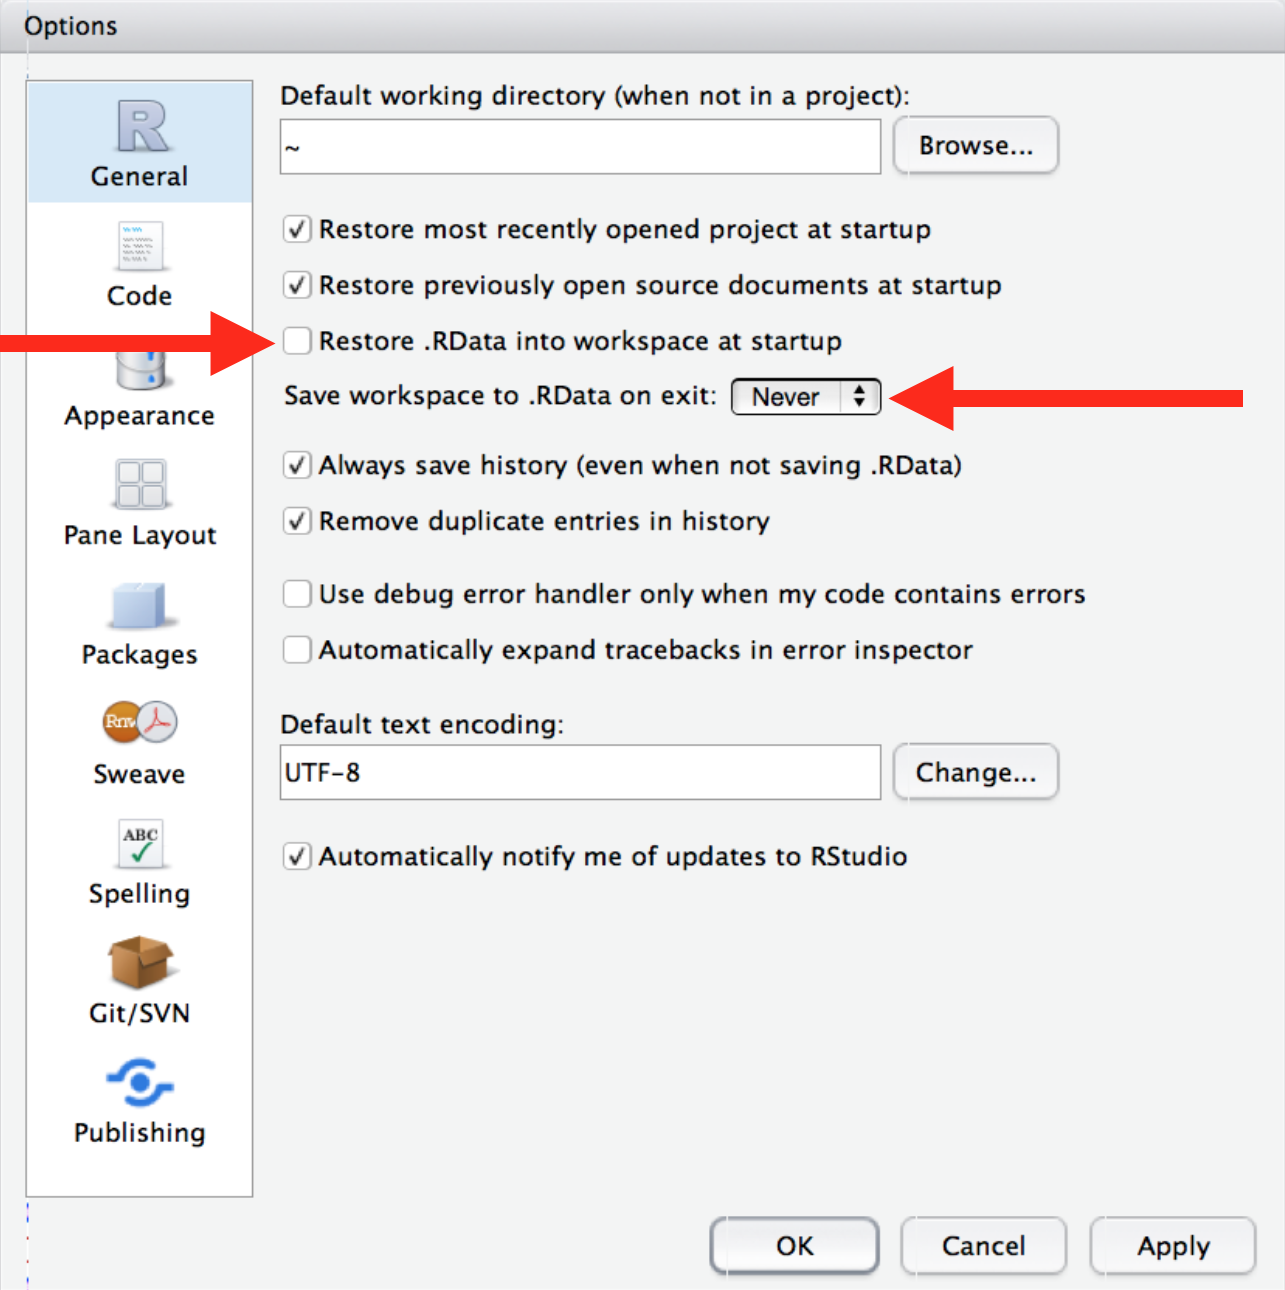
\includegraphics{img/rstudio-workspace.png}
\caption{}
\end{figure}

This will cause you some short-term pain, because now when you restart
RStudio, it will not remember the results of the code that you ran last
time. But this short-term pain will save you long-term agony, because it
forces you to capture all important interactions in your scripts.

\subsection{Working Directories and
Paths}\label{working-directories-and-paths}

Like many programming languages, R has a powerful notion of the
\textbf{working directory}. This is where R looks for files that you ask
it to load, and where it will put any files that you ask it to save.

RStudio shows your current working directory at the top of the console.
You can print this out in R code by running \texttt{getwd()}:

\begin{Shaded}
\begin{Highlighting}[]
\KeywordTok{getwd}\NormalTok{()}
\CommentTok{#> [1] "/Users/rochelleterman/Desktop/plsc-31101"}
\end{Highlighting}
\end{Shaded}

I do not recommend it, but you can set the working directory from within
R:

\begin{Shaded}
\begin{Highlighting}[]
\KeywordTok{setwd}\NormalTok{(}\StringTok{"/path/to/my/CoolProject"}\NormalTok{)}
\end{Highlighting}
\end{Shaded}

The command above prints out a \textbf{path} to your working directory.
Think of a path as an address. Paths are incredibly important in
programming, but can be a little tricky. So let's go into a big more
detail.

\subsubsection*{Absolute paths.}\label{absolute-paths.}
\addcontentsline{toc}{subsubsection}{Absolute paths.}

Absolute paths are paths that point to the same place regardless of your
current working directory. They always start with the \textbf{root
directory} that holds everything else on your computer.

\begin{itemize}
\tightlist
\item
  In Windows, absolute paths start with a drive letter (e.g.
  \texttt{C:}) or two backslashes (e.g.
  \texttt{\textbackslash{}\textbackslash{}servername}).
\item
  In Mac/Linux they start with a slash \texttt{/}. This is the leading
  alsh in \texttt{/users/rterman}.
\end{itemize}

Inside the root directory are several other directories, which we call
\textbf{subdirectories}. We know that the directory
\texttt{/home/rterman} is stored inside \texttt{/home} because
\texttt{/home} is the first part of its name. Similarly, we know that
\texttt{/home} is stored inside the root directory \texttt{/} because
its name begins with \texttt{/}.

\begin{quote}
Notice that there are two meanings for the \texttt{/} character. When it
appears at the front of a file or directory name, it refers to the root
directory. When it appears \emph{inside} a name, it's just a separator.
\end{quote}

\subsubsection*{Mac/Linux vs.~Windows}\label{maclinux-vs.windows}
\addcontentsline{toc}{subsubsection}{Mac/Linux vs.~Windows}

There are two basic styles of paths: Mac/Linux and Windows. The main
difference is how you separate the components of the path. Mac and Linux
uses slashes (e.g. \texttt{plots/diamonds.pdf}) and Windows uses
backslashes (e.g. \texttt{plots\textbackslash{}diamonds.pdf}).

R can work with either type, no matter what platform you're currently
using. Unfortunately, backslashes mean something special to R, and to
get a single backslash in the path, you need to type two backslashes!
That makes life frustrating, so I recommend always using the Linux/Mac
style with forward slashes.

\subsubsection*{Home Directory}\label{home-directory}
\addcontentsline{toc}{subsubsection}{Home Directory}

Sometimes you'll see a \texttt{\textasciitilde{}} character in a path. *
In Mac/Linux, the \texttt{\textasciitilde{}} is a convenient shortcut to
your \textbf{home directory} (\texttt{/users/rterman}). * Windows
doesn't really have the notion of a home directory, so it usually points
to your documents directory (\texttt{C:\textbackslash{}Documents} and
\texttt{Settings\textbackslash{}rterman})

\subsubsection*{Absolute vs.~Relative
Paths}\label{absolute-vs.relative-paths}
\addcontentsline{toc}{subsubsection}{Absolute vs.~Relative Paths}

You should try not to use absolute paths in your scripts, because they
hinder sharing: no one else will have exactly the same directory
configuration as you. Another way to direct R to something is to give it
a \textbf{relative pth}.

Relative paths point to something relatively to where we are, rather
than from the root of the file system. For example, if our current
working directory is \texttt{/home/rterman}, then the relatively path
\texttt{data/un.csv} directs to the full absolute path:
\texttt{/home/rterman/data/un.csv}

\subsection{R Projects}\label{r-projects}

As a beginning R user, it's OK to let your home directory, documents
directory, or any other weird directory on your computer be R's working
directory.

But from this point forward, you should be organizing your projects into
dedicated subdirectories, containing all the files associated with a
project --- input data, R scripts, results, figures.

This is such a common practice that RStudio has built-in support for
this via \textbf{projects}.

Let's make a project togeteher. Click
\texttt{File\ \textgreater{}\ New\ Project}, then:

\textasciitilde{}\href{rstudio-project-1.png}{}

Think carefully about which subdirectory you put the project in. If you
don't store it somewhere sensible, it will be hard to find it in the
future!

Once this process is complete, you'll get a new RStudio project. Check
that the ``home'' directory of your project is the current working
directory:

\begin{Shaded}
\begin{Highlighting}[]
\KeywordTok{getwd}\NormalTok{()}
\CommentTok{#> [1] "/Users/rochelleterman/Desktop/plsc-31101"}
\end{Highlighting}
\end{Shaded}

Now ehenever you refer to a file with a relative path, it will look for
it there.

Go ahead and create an new R script and save it inside the project
folder.

Quit RStudio. Inspect the folder associated with your project --- notice
the .Rproj file. Double-click that file to re-open the project. Notice
you get back to where you left off: it's the same working directory and
command history, and all the files you were working on are still open.
Because you followed my instructions above, you will, however, have a
completely fresh environment, guaranteeing that you're starting with a
clean slate.

\subsection{File Organization}\label{file-organization}

You should be saving all your files associated with your project in one
directory. Here's a basic organization structure that I recommend:

\begin{Shaded}
\begin{Highlighting}[]
\NormalTok{~~~}
\NormalTok{masters_thesis:}
\NormalTok{  masters_thesis.Rproj}
\NormalTok{  01_Clean.R}
\NormalTok{  02_Model.R}
\NormalTok{  03_Visualizations.R}
\NormalTok{  Data/}
\BaseNTok{    raw/}
\BaseNTok{      un-raw.csv}
\BaseNTok{      worldbank-raw.csv}
\BaseNTok{    cleaned/}
\BaseNTok{      country-year.csv}
\NormalTok{  Results:}
\BaseNTok{    regressions}
\BaseNTok{      h1.txt}
\BaseNTok{      h2.txt}
\BaseNTok{    figures}
\BaseNTok{      bivariate.pdf}
\BaseNTok{      bar_plot.pdf}
\NormalTok{~~~}
\end{Highlighting}
\end{Shaded}

Here are some important tips:

\begin{itemize}
\tightlist
\item
  read raw data in from the \texttt{Data} subdirectory. Don't ever
  change or overwrite the raw data!
\item
  export cleaned and altered data into a separate directory.
\item
  write separate scripts for each stage in the research pipeline. Keep
  scripts short and focused on one main purpose. If a script gets too
  long, that might be a sign you need to split it up.
\item
  write scripts that reproduce your results and figures, and write them
  in the \texttt{Results} subdirectory.
\end{itemize}

\subsubsection*{Acknowledgements}\label{acknowledgements}
\addcontentsline{toc}{subsubsection}{Acknowledgements}

This page is in part derived from the following sources:

\begin{enumerate}
\def\labelenumi{\arabic{enumi}.}
\tightlist
\item
  \href{https://r4ds.had.co.nz}{R for Data Science} licensed under
  \href{https://creativecommons.org/licenses/by-nc-nd/3.0/us/}{Creative
  Commons Attribution-NonCommercial-NoDerivs 3.0}
\end{enumerate}

\subsubsection*{More Resources}\label{more-resources}
\addcontentsline{toc}{subsubsection}{More Resources}

\begin{itemize}
\tightlist
\item
  \href{https://web.stanford.edu/~gentzkow/research/CodeAndData.pdf}{Gentzkow,
  Matthew and Jesse M. Shapiro. 2014. Code and Data for the Social
  Sciences: A Practitioner's Guide.}
\end{itemize}

\section{Introduction to Data}\label{introduction-to-data}

The following weeks will be focused on using R for data cleaning and
analysis. Let's first get on the same page on some terms:

\begin{itemize}
\item
  A \textbf{variable} is a quantity, quality, or property that you can
  measure.
\item
  An \textbf{observation} is a set of measurements for the same unit. An
  observation will contain several values, each associated with a
  different variable. I'll sometimes refer to an observation as a
  \textbf{data point} or an \textbf{element}.
\item
  A \textbf{value} is the state of a variable for a particular
  observation.
\item
  \textbf{Tabular data} is a set of values, each associated with a
  variable and an observation. Tabular data has rows (observations) and
  columns (variables). Also called \emph{rectangular} data or
  \emph{spreadsheets.}
\end{itemize}

\begin{figure}
\centering
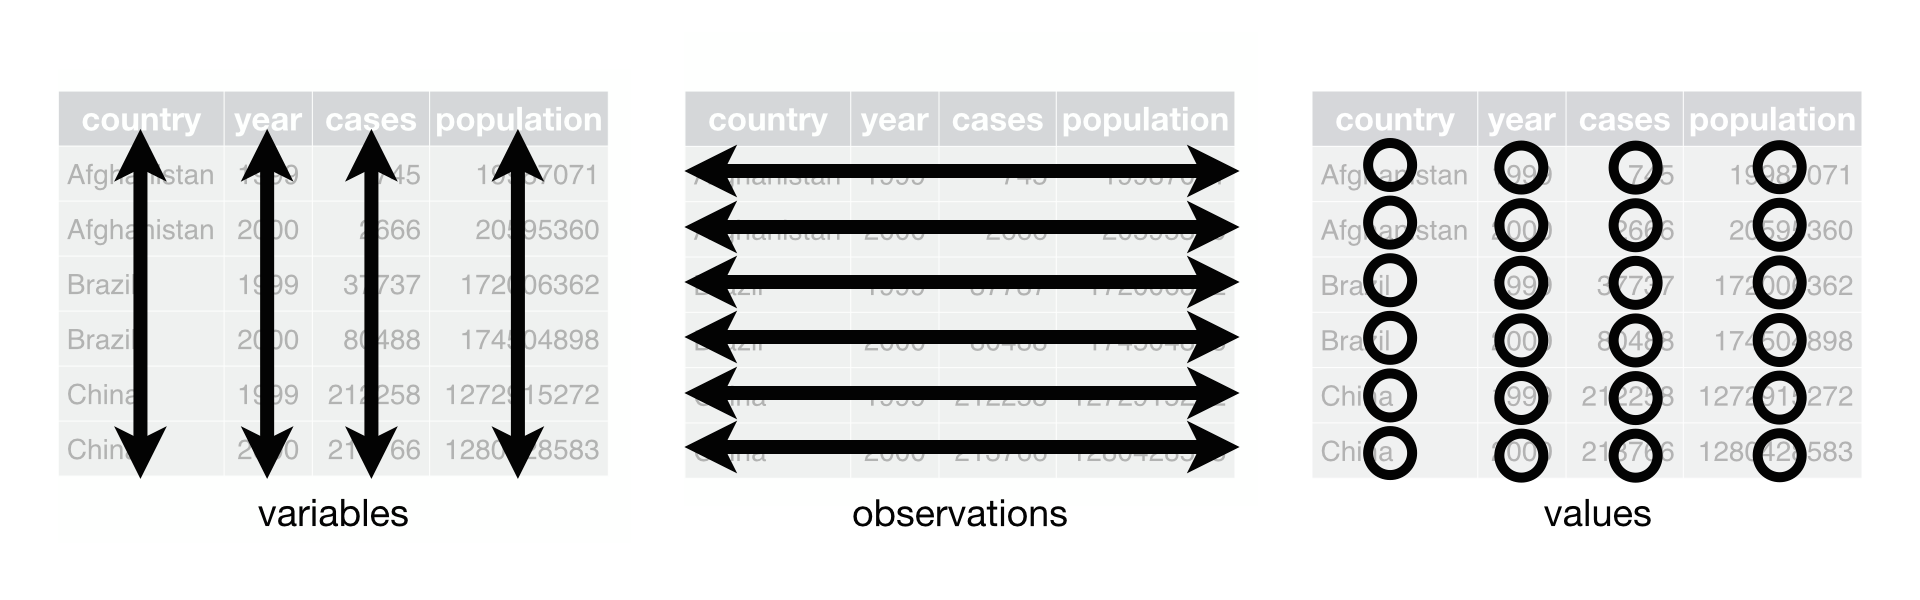
\includegraphics{img/tidy-1.png}
\caption{}
\end{figure}

\subsection{Where's my data?}\label{wheres-my-data}

To start, you first need to know where your data lives. Sometimes, the
data is stored as a file on your computer, e.g.~csv, Excel, SPSS, or
some other file type. When the data is on your computer, we say the data
is stored \textbf{locally}.

Data can also stored externally on the Internet, in a package, or
obtained through other sources. For example, some R packages contain
datasets. The \texttt{nycflights13} package contains information on
flights that departed NYC in 2013.

\begin{Shaded}
\begin{Highlighting}[]
\CommentTok{# not run}
\CommentTok{# install.packages("nycflights13")}
\KeywordTok{library}\NormalTok{(nycflights13)}
\KeywordTok{data}\NormalTok{(flights)}
\KeywordTok{names}\NormalTok{(flights)}
\CommentTok{#>  [1] "year"           "month"          "day"            "dep_time"      }
\CommentTok{#>  [5] "sched_dep_time" "dep_delay"      "arr_time"       "sched_arr_time"}
\CommentTok{#>  [9] "arr_delay"      "carrier"        "flight"         "tailnum"       }
\CommentTok{#> [13] "origin"         "dest"           "air_time"       "distance"      }
\CommentTok{#> [17] "hour"           "minute"         "time_hour"}
\KeywordTok{rm}\NormalTok{(flights)}
\CommentTok{# }
\end{Highlighting}
\end{Shaded}

Later in this course, we'll discuss how to obtain data from the web APIs
and websites. For now, the rest of the unit discusses data that is
stored \textbf{locally}.

\subsection{Data storage}\label{data-storage}

Ideally, your data should be stored in a certain file format. I
recommend a \texttt{csv} (comma separated value) file, which formats
spreadsheet (rectangular) data in a plain-text format. \texttt{csv}
files are plain-text, and can be read into almost any statistical
software program, including R. Try to avoid Excel files if you can.

Here are some other tips:

\begin{itemize}
\tightlist
\item
  When working with spreadsheets, the first row is usually reserved for
  the header, while the first column is used to identify the sampling
  unit (\textbf{unique identifier}, see below.)
\item
  Avoid file names and variable names with blank spaces. This can cause
  errors when reading in data.
\item
  If you want to concatenate words, inserting a \texttt{.} or
  \texttt{\_} in between to words instead of a space;
\item
  Short names are prefered over longer names;
\item
  Try to avoid using names that contain symbols such as \texttt{?},
  \texttt{\$},\texttt{\%}, \texttt{\^{}}, \texttt{\&}, \texttt{*},
  \texttt{(}, \texttt{)}, \texttt{-}, \texttt{\#}, \texttt{?},
  \texttt{,}, \texttt{\textless{}}, \texttt{\textgreater{}}, \texttt{/},
  \texttt{\textbar{}}, \texttt{\textbackslash{}}, \texttt{{[}}
  ,\texttt{{]}},\texttt{\{}, and \texttt{\}};
\item
  make sure that any missing values in your data set are indicated with
  \texttt{NA} or blank fields (don't use 99 or 77)..
\end{itemize}

\subsection{\texorpdfstring{\texttt{tidy}
data}{tidy data}}\label{tidy-data}

Datasets in the wild can often be messy. For example, check out the
following data.

\begin{Shaded}
\begin{Highlighting}[]
\NormalTok{messy <-}\StringTok{ }\KeywordTok{data.frame}\NormalTok{(}
  \DataTypeTok{county =} \KeywordTok{c}\NormalTok{(}\DecValTok{36037}\NormalTok{, }\DecValTok{36038}\NormalTok{, }\DecValTok{36039}\NormalTok{, }\DecValTok{36040}\NormalTok{, }\OtherTok{NA}\NormalTok{ , }\DecValTok{37001}\NormalTok{, }\DecValTok{37002}\NormalTok{, }\DecValTok{37003}\NormalTok{),}
  \DataTypeTok{state =} \KeywordTok{c}\NormalTok{(}\StringTok{'NY'}\NormalTok{, }\StringTok{'NY'}\NormalTok{, }\StringTok{'NY'}\NormalTok{, }\OtherTok{NA}\NormalTok{, }\OtherTok{NA}\NormalTok{, }\StringTok{'VA'}\NormalTok{, }\StringTok{'VA'}\NormalTok{, }\StringTok{'VA'}\NormalTok{),}
  \DataTypeTok{cnty_pop =} \KeywordTok{c}\NormalTok{(}\DecValTok{3817735}\NormalTok{, }\DecValTok{422999}\NormalTok{, }\DecValTok{324920}\NormalTok{, }\DecValTok{143432}\NormalTok{, }\OtherTok{NA}\NormalTok{, }\DecValTok{3228290}\NormalTok{, }\DecValTok{449499}\NormalTok{, }\DecValTok{383888}\NormalTok{),}
  \DataTypeTok{state_pop =} \KeywordTok{c}\NormalTok{(}\DecValTok{43320903}\NormalTok{, }\DecValTok{43320903}\NormalTok{, }\OtherTok{NA}\NormalTok{, }\DecValTok{43320903}\NormalTok{, }\DecValTok{43320903}\NormalTok{, }\DecValTok{7173000}\NormalTok{, }\DecValTok{7173000}\NormalTok{, }\DecValTok{7173000}\NormalTok{),}
  \DataTypeTok{region =} \KeywordTok{c}\NormalTok{(}\DecValTok{1}\NormalTok{, }\DecValTok{1}\NormalTok{, }\DecValTok{1}\NormalTok{, }\DecValTok{1}\NormalTok{, }\DecValTok{1}\NormalTok{, }\DecValTok{3}\NormalTok{, }\DecValTok{3}\NormalTok{, }\DecValTok{4}\NormalTok{)}
\NormalTok{)}
\NormalTok{messy}
\CommentTok{#>   county state cnty_pop state_pop region}
\CommentTok{#> 1  36037    NY  3817735  43320903      1}
\CommentTok{#> 2  36038    NY   422999  43320903      1}
\CommentTok{#> 3  36039    NY   324920        NA      1}
\CommentTok{#> 4  36040  <NA>   143432  43320903      1}
\CommentTok{#> 5     NA  <NA>       NA  43320903      1}
\CommentTok{#> 6  37001    VA  3228290   7173000      3}
\CommentTok{#> 7  37002    VA   449499   7173000      3}
\CommentTok{#> 8  37003    VA   383888   7173000      4}
\end{Highlighting}
\end{Shaded}

What a mess! How can the population of the state of New York be 43
million for one county but ``missing'' for another? If this is a dataset
of counties, what does it mean when the ``county'' field is missing? If
region is something like Census region, how can two counties in the same
state be in different regions? And why is it that all the counties whose
codes start with 36 are in New York except for one, where the state is
unknown?

The goal should be to put our data in a tidy format. The two most
important properties of tidy data are:

\begin{enumerate}
\def\labelenumi{\arabic{enumi}.}
\tightlist
\item
  Each variable forms a column.
\item
  Each observation forms a row.
\item
  Each type of observational unit forms a table.
\end{enumerate}

If we follow these principles, our data should look like:

\begin{Shaded}
\begin{Highlighting}[]
\NormalTok{counties <-}\StringTok{ }\KeywordTok{data.frame}\NormalTok{(}
  \DataTypeTok{county =} \KeywordTok{c}\NormalTok{(}\DecValTok{36037}\NormalTok{, }\DecValTok{36038}\NormalTok{, }\DecValTok{36039}\NormalTok{, }\DecValTok{36040}\NormalTok{, }\DecValTok{37001}\NormalTok{, }\DecValTok{37002}\NormalTok{, }\DecValTok{37003}\NormalTok{),}
  \DataTypeTok{state =} \KeywordTok{c}\NormalTok{(}\StringTok{'NY'}\NormalTok{, }\StringTok{'NY'}\NormalTok{, }\StringTok{'NY'}\NormalTok{, }\StringTok{'NY'}\NormalTok{, }\StringTok{'VA'}\NormalTok{, }\StringTok{'VA'}\NormalTok{, }\StringTok{'VA'}\NormalTok{),}
  \DataTypeTok{population =} \KeywordTok{c}\NormalTok{(}\DecValTok{3817735}\NormalTok{, }\DecValTok{422999}\NormalTok{, }\DecValTok{324920}\NormalTok{, }\DecValTok{143432}\NormalTok{, }\DecValTok{3228290}\NormalTok{, }\DecValTok{449499}\NormalTok{, }\DecValTok{383888}\NormalTok{)}
\NormalTok{)}
\NormalTok{counties}
\CommentTok{#>   county state population}
\CommentTok{#> 1  36037    NY    3817735}
\CommentTok{#> 2  36038    NY     422999}
\CommentTok{#> 3  36039    NY     324920}
\CommentTok{#> 4  36040    NY     143432}
\CommentTok{#> 5  37001    VA    3228290}
\CommentTok{#> 6  37002    VA     449499}
\CommentTok{#> 7  37003    VA     383888}

\NormalTok{states <-}\StringTok{ }\KeywordTok{data.frame}\NormalTok{(}
  \DataTypeTok{state =} \KeywordTok{c}\NormalTok{(}\StringTok{"NY"}\NormalTok{, }\StringTok{"VA"}\NormalTok{),}
  \DataTypeTok{population =} \KeywordTok{c}\NormalTok{(}\DecValTok{43320903}\NormalTok{, }\DecValTok{7173000}\NormalTok{),}
  \DataTypeTok{region =} \KeywordTok{c}\NormalTok{(}\DecValTok{1}\NormalTok{, }\DecValTok{3}\NormalTok{)}
\NormalTok{)}
\NormalTok{states}
\CommentTok{#>   state population region}
\CommentTok{#> 1    NY   43320903      1}
\CommentTok{#> 2    VA    7173000      3}
\end{Highlighting}
\end{Shaded}

Now the ambiguity is gone. Every county has a population and a state.
Every state has a population and a region. There are no missing states,
no missing counties, and no conflicting definitions. The database is
self-documenting. In fact, the database is now so clear that we can
forget about names like county\_pop and state\_pop and just stick to
``population.'' Anyone would know which entity's population you mean.

We'll talk more about tidying data in later units.

\subsection{Relational data}\label{relational-data}

Collectively, multiple tables of data are called \textbf{relational
data} because it is the relations, not just the individual datasets,
that are important. Note that when we say relational database here, we
are referring to how the data are structured, not to the use of any
fancy software.

The main principle of relational data is that each table is structured
around the same observational unit.

\begin{itemize}
\tightlist
\item
  counties contains data on counties.
\item
  states contains data on states
\end{itemize}

County population is a property of a county, so it lives in the county
table. State population is a property of a state, so it cannot live in
the county table. If we had panel data on counties, we would need
separate tables for things that vary at the county level (like state)
and things that vary at the county-year level (like population).

\subsection{Keys}\label{keys}

The variables used to connect each pair of tables are called
\textbf{keys}. A key is a variable (or set of variables) that uniquely
identifies an observation. Also called a \emph{unique identifier}.

\begin{itemize}
\tightlist
\item
  Keys are complete. They never take on missing values.
\item
  Keys are unique. They are neer duplicated across rows of a table.
\end{itemize}

In simple cases, a single variable is sufficient to identify an
observation. In the example above, each county is identified with
\textbf{county} (a numeric identifier); each state is identified with
\textbf{state} (a two-letter string).

There are two types of keys:

\begin{itemize}
\item
  A \textbf{primary key} uniquely identifies an observation in its own
  table. For example, \texttt{counties\$county} is a primary key because
  it uniquely identifies each county in the counties table.
\item
  A \textbf{foreign key} uniquely identifies an observation in another
  table. For example, the counties\$state is a foreign key because it
  appears in the counties table where it matches each county to a unique
  state.
\end{itemize}

A primary key and the corresponding foreign key in another table form a
\textbf{relation}.

Sometimes a table doesn't have an explicit primary key: each row is an
observation, but no combination of variables reliably identifies it. If
a table lacks a primary key, it's useful to add one.

\subsubsection*{Acknowledgements}\label{acknowledgements-1}
\addcontentsline{toc}{subsubsection}{Acknowledgements}

This page is in part derived from the following sources:

\begin{enumerate}
\def\labelenumi{\arabic{enumi}.}
\item
  \href{https://r4ds.had.co.nz}{R for Data Science} licensed under
  \href{https://creativecommons.org/licenses/by-nc-nd/3.0/us/}{Creative
  Commons Attribution-NonCommercial-NoDerivs 3.0}
\item
  \href{https://web.stanford.edu/~gentzkow/research/CodeAndData.pdf}{Gentzkow,
  Matthew and Jesse M. Shapiro. 2014. Code and Data for the Social
  Sciences: A Practitioner's Guide.}
\end{enumerate}

\section{Importing and Exporting}\label{importing-and-exporting}

\subsection{Importing Data}\label{importing-data}

\subsubsection*{Find paths first.}\label{find-paths-first.}
\addcontentsline{toc}{subsubsection}{Find paths first.}

In order to import (or read) data into R, you first have to know where
it is, and how to find it.

First, remember that you'll need to know the \emph{current working
directory} so that you know where R is looking for files. If you're
using R Projects, that working directory will be the top-level directory
of the project.

Second, you'll need to know where the data file is, relative to your
working directory. If it's stored in the \texttt{Data/raw/} folder, the
relative path to your file will be \texttt{Data/raw/file-name.csv}

\subsubsection*{Reading Tabular Data}\label{reading-tabular-data}
\addcontentsline{toc}{subsubsection}{Reading Tabular Data}

The workhorse for reading into a data frame is \emph{read.table()},
which allows any separator (CSV, tab-delimited, etc.). \emph{read.csv()}
is a special case of \emph{read.table()} for CSV files.

The basic formula is:

\begin{Shaded}
\begin{Highlighting}[]
\CommentTok{# Basic CSV read: Import data with header row, values separated by ",", decimals as "."}
\NormalTok{mydataset <-}\StringTok{ }\KeywordTok{read.csv}\NormalTok{(}\DataTypeTok{file=}\StringTok{"  "}\NormalTok{, }\DataTypeTok{stringsAsFactors=}\NormalTok{)}
\end{Highlighting}
\end{Shaded}

Here's a practical example, using the polityVI dataset:

\begin{Shaded}
\begin{Highlighting}[]
\CommentTok{#import polity}
\NormalTok{polity <-}\StringTok{ }\KeywordTok{read.csv}\NormalTok{(}\StringTok{"data/polity.csv"}\NormalTok{, }\DataTypeTok{stringsAsFactors =}\NormalTok{ F)}
\NormalTok{polity[}\DecValTok{1}\OperatorTok{:}\DecValTok{5}\NormalTok{, }\DecValTok{1}\OperatorTok{:}\DecValTok{5}\NormalTok{]}
\CommentTok{#>     cyear ccode scode     country year}
\CommentTok{#> 1 7001800   700   AFG Afghanistan 1800}
\CommentTok{#> 2 7001801   700   AFG Afghanistan 1801}
\CommentTok{#> 3 7001802   700   AFG Afghanistan 1802}
\CommentTok{#> 4 7001803   700   AFG Afghanistan 1803}
\CommentTok{#> 5 7001804   700   AFG Afghanistan 1804}
\end{Highlighting}
\end{Shaded}

We use \texttt{stringsAsFactors\ =\ F} in order to treat text columns as
character vectors, not as factors. If we don't set this, the default is
that all non-numerical columns will be encoded as factors. This behavior
usually makes poor sense, and is due to historical reasons. At one point
in time, factors were faster than character vectors, so R's
\texttt{read.table()} set the default to read in text as factors.

\texttt{read.table()} has a number of other options:

\begin{Shaded}
\begin{Highlighting}[]
\CommentTok{# For importing tabular data with maximum customizeability}
\NormalTok{mydataset <-}\StringTok{ }\KeywordTok{read.table}\NormalTok{(}\DataTypeTok{file=}\NormalTok{, }\DataTypeTok{header=}\NormalTok{, }\DataTypeTok{sep=}\NormalTok{, }\DataTypeTok{quote=}\NormalTok{, }\DataTypeTok{dec=}\NormalTok{, }\DataTypeTok{fill=}\NormalTok{, }\DataTypeTok{stringsAsFactors=}\NormalTok{)}
\end{Highlighting}
\end{Shaded}

\subsubsection*{Reading Excel files}\label{reading-excel-files}
\addcontentsline{toc}{subsubsection}{Reading Excel files}

Don't use Microsoft Excel file (.xls or .xlsx). But if you must:

\begin{Shaded}
\begin{Highlighting}[]
\CommentTok{# Make sure you have installed the tidyverse suite (only necessary one time)}
\CommentTok{# install.packages("tidyverse") # Not Run}

\CommentTok{# Load the "readxl" package (necessary every new R session)}
\KeywordTok{library}\NormalTok{(readxl)}
\end{Highlighting}
\end{Shaded}

\texttt{read\_excel()} reads both \texttt{xls} and \texttt{xlsx} files
and detects the format from the extension.

\begin{Shaded}
\begin{Highlighting}[]
\CommentTok{# Basic call}
\NormalTok{mydataset <-}\StringTok{ }\KeywordTok{read_excel}\NormalTok{(}\DataTypeTok{path =}\NormalTok{ , }\DataTypeTok{sheet =} \StringTok{")}
\end{Highlighting}
\end{Shaded}

Here's a real example:

\begin{Shaded}
\begin{Highlighting}[]
\CommentTok{# Example with .xlsx (single sheet)}
\NormalTok{air <-}\StringTok{ }\KeywordTok{read_excel}\NormalTok{(}\StringTok{"data/airline_small.xlsx"}\NormalTok{, }\DataTypeTok{sheet =} \DecValTok{1}\NormalTok{) }
\NormalTok{air[}\DecValTok{1}\OperatorTok{:}\DecValTok{5}\NormalTok{, }\DecValTok{1}\OperatorTok{:}\DecValTok{5}\NormalTok{]}
\CommentTok{#> # A tibble: 5 x 5}
\CommentTok{#>    Year Month DayofMonth DayOfWeek DepTime}
\CommentTok{#>   <dbl> <dbl>      <dbl>     <dbl> <chr>  }
\CommentTok{#> 1  2005    11         22         2 1700   }
\CommentTok{#> 2  2008     1         31         4 2216   }
\CommentTok{#> 3  2005     7         17         7 905    }
\CommentTok{#> 4  2008     9         23         2 859    }
\CommentTok{#> 5  2005     3          5         6 827}
\end{Highlighting}
\end{Shaded}

\subsubsection*{Reading Stata (.dta)
files}\label{reading-stata-.dta-files}
\addcontentsline{toc}{subsubsection}{Reading Stata (.dta) files}

There are many ways to read \texttt{.dta} files into R. I recommend
using \texttt{haven} because it is part of the \texttt{tidyverse.}

\begin{Shaded}
\begin{Highlighting}[]
\KeywordTok{library}\NormalTok{(haven)}
\NormalTok{air.dta <-}\StringTok{ }\KeywordTok{read_dta}\NormalTok{(}\StringTok{"data/airline_small.dta"}\NormalTok{) }
\NormalTok{air[}\DecValTok{1}\OperatorTok{:}\DecValTok{5}\NormalTok{, }\DecValTok{1}\OperatorTok{:}\DecValTok{5}\NormalTok{]}
\CommentTok{#> # A tibble: 5 x 5}
\CommentTok{#>    Year Month DayofMonth DayOfWeek DepTime}
\CommentTok{#>   <dbl> <dbl>      <dbl>     <dbl> <chr>  }
\CommentTok{#> 1  2005    11         22         2 1700   }
\CommentTok{#> 2  2008     1         31         4 2216   }
\CommentTok{#> 3  2005     7         17         7 905    }
\CommentTok{#> 4  2008     9         23         2 859    }
\CommentTok{#> 5  2005     3          5         6 827}
\end{Highlighting}
\end{Shaded}

\subsubsection*{For really big data}\label{for-really-big-data}
\addcontentsline{toc}{subsubsection}{For really big data}

If you have really big data, \texttt{read.csv()} will be too slow. In
these cases, check out the following options:

1.) \texttt{read\_csv()} in the \texttt{readr} package is a faster, more
helpful drop-in replacement for \texttt{read.csv()} that plays well with
tidyverse packages (discussed in future lessons). 2) the
\texttt{data.table} package is great for reading and manipulating large
datasets (orders of gigabytes or 10s of gigabytes)

\subsection{Exporting data}\label{exporting-data}

You should never go from raw data to results in one script. Typically,
you'll want to import raw data, clean it, and then export that cleaned
dataset onto your computer. That cleaned dataset will then be imported
into another script for analysis, in a modular fashion.

To export (or write) data from R onto your computer, you can create
individual \texttt{.csv} files, or export many data objects into an
\texttt{.RData} object.

\subsubsection*{\texorpdfstring{Writing a \texttt{csv}
spreadsheet.}{Writing a csv spreadsheet.}}\label{writing-a-csv-spreadsheet.}
\addcontentsline{toc}{subsubsection}{Writing a \texttt{csv}
spreadsheet.}

To export an individual dataframe as a spreadsheet, use
\texttt{write.csv()}

\begin{Shaded}
\begin{Highlighting}[]
\CommentTok{# Basic call}
\KeywordTok{write.csv}\NormalTok{(}\DataTypeTok{x =}\NormalTok{ , }\DataTypeTok{file =}\NormalTok{ , }\DataTypeTok{row.names =}\NormalTok{ , }\DataTypeTok{col.names =}\NormalTok{)}
\end{Highlighting}
\end{Shaded}

Let's write the \texttt{air} dataset as a csv.

\begin{Shaded}
\begin{Highlighting}[]
\CommentTok{# Basic call}
\KeywordTok{write.csv}\NormalTok{(air, }\StringTok{"data/airlines.csv"}\NormalTok{, }\DataTypeTok{row.names =}\NormalTok{ F)}
\end{Highlighting}
\end{Shaded}

\subsubsection*{Packaging data into
.RData}\label{packaging-data-into-.rdata}
\addcontentsline{toc}{subsubsection}{Packaging data into .RData}

Sometimes, it's helpful to write several dataframes at once, to be used
in later analysis. To do so, we use the \texttt{save()} function to
create one file containing many R data objects.

\begin{Shaded}
\begin{Highlighting}[]
\CommentTok{# Basic call}
\KeywordTok{save}\NormalTok{(..., }\DataTypeTok{file =}\NormalTok{ )}
\end{Highlighting}
\end{Shaded}

Here's how we can write both \texttt{air} and \texttt{polity} into one
file.

\begin{Shaded}
\begin{Highlighting}[]
\KeywordTok{save}\NormalTok{(air, polity, }\DataTypeTok{file =} \StringTok{"data/datasets.RData"}\NormalTok{)}
\end{Highlighting}
\end{Shaded}

We can then read these datasets back into R using \texttt{load()}

\begin{Shaded}
\begin{Highlighting}[]
\CommentTok{# clear environment}
\KeywordTok{rm}\NormalTok{(}\DataTypeTok{list=}\KeywordTok{ls}\NormalTok{())}

\CommentTok{# load datasets}
\KeywordTok{load}\NormalTok{(}\StringTok{"data/datasets.RData"}\NormalTok{)}
\end{Highlighting}
\end{Shaded}

\section{Exploring Data}\label{exploring-data}

\subsection{The Gapminder dataset}\label{the-gapminder-dataset}

This lessons discusses how to perform basic exploratory data analysis.

For this unit, we'll be working with the ``Gapminder'' dataset, which is
excerpt of the data available at Gapminder.org. For each of 142
countries, the data provides values for life expectancy, GDP per capita,
and population, every five years, from 1952 to 2007.

\begin{Shaded}
\begin{Highlighting}[]
\NormalTok{gap <-}\StringTok{ }\KeywordTok{read.csv}\NormalTok{(}\StringTok{"data/gapminder.csv"}\NormalTok{, }\DataTypeTok{stringsAsFactors =}\NormalTok{ F)}
\end{Highlighting}
\end{Shaded}

\subsection{Structure and Dimensions}\label{structure-and-dimensions}

The very first thing we want to know about a dataset are its dimensions
and basic structure. For instance we can look at the number of rows and
columns:

\begin{Shaded}
\begin{Highlighting}[]
\CommentTok{# get number of rows and columns:}
\KeywordTok{dim}\NormalTok{(gap)}
\CommentTok{#> [1] 1704    6}
\end{Highlighting}
\end{Shaded}

We might also want to see the names of the columns:

\begin{Shaded}
\begin{Highlighting}[]
\CommentTok{# see column names}
\KeywordTok{names}\NormalTok{(gap)}
\CommentTok{#> [1] "country"   "year"      "pop"       "continent" "lifeExp"   "gdpPercap"}
\end{Highlighting}
\end{Shaded}

The \texttt{str} function is helpful to see an overview of the data's
structure:

\begin{Shaded}
\begin{Highlighting}[]
\CommentTok{# see structure of data}
\KeywordTok{str}\NormalTok{(gap)}
\CommentTok{#> 'data.frame':    1704 obs. of  6 variables:}
\CommentTok{#>  $ country  : chr  "Afghanistan" "Afghanistan" "Afghanistan" "Afghanistan" ...}
\CommentTok{#>  $ year     : int  1952 1957 1962 1967 1972 1977 1982 1987 1992 1997 ...}
\CommentTok{#>  $ pop      : num  8425333 9240934 10267083 11537966 13079460 ...}
\CommentTok{#>  $ continent: chr  "Asia" "Asia" "Asia" "Asia" ...}
\CommentTok{#>  $ lifeExp  : num  28.8 30.3 32 34 36.1 ...}
\CommentTok{#>  $ gdpPercap: num  779 821 853 836 740 ...}
\end{Highlighting}
\end{Shaded}

Finally, I encourage you to actually peak at the data itself. The
\texttt{head} function displays the first 6 rows of any dataframe.

\begin{Shaded}
\begin{Highlighting}[]
\KeywordTok{head}\NormalTok{(gap)}
\CommentTok{#>       country year      pop continent lifeExp gdpPercap}
\CommentTok{#> 1 Afghanistan 1952  8425333      Asia    28.8       779}
\CommentTok{#> 2 Afghanistan 1957  9240934      Asia    30.3       821}
\CommentTok{#> 3 Afghanistan 1962 10267083      Asia    32.0       853}
\CommentTok{#> 4 Afghanistan 1967 11537966      Asia    34.0       836}
\CommentTok{#> 5 Afghanistan 1972 13079460      Asia    36.1       740}
\CommentTok{#> 6 Afghanistan 1977 14880372      Asia    38.4       786}
\end{Highlighting}
\end{Shaded}

\subsection{Common alterations}\label{common-alterations}

There are some very common alterations researchs make on their data:
changing column names, assigning NA values, changing column type.

Note that we will be cover how to perform these functions using
\texttt{tidyverse} later in the course. However, these lines are very
common, so it's good to know how they work:

\begin{enumerate}
\def\labelenumi{\arabic{enumi}.}
\tightlist
\item
  change column names
\end{enumerate}

\begin{Shaded}
\begin{Highlighting}[]
\KeywordTok{names}\NormalTok{(gap)}
\CommentTok{#> [1] "country"   "year"      "pop"       "continent" "lifeExp"   "gdpPercap"}
\KeywordTok{names}\NormalTok{(gap) <-}\StringTok{ }\KeywordTok{c}\NormalTok{(}\StringTok{"country"}\NormalTok{, }\StringTok{"year"}\NormalTok{, }\StringTok{"pop"}\NormalTok{, }\StringTok{"continent"}\NormalTok{, }\StringTok{"life.exp"}\NormalTok{, }\StringTok{"gdp.percap"}\NormalTok{)}
\KeywordTok{str}\NormalTok{(gap)}
\CommentTok{#> 'data.frame':    1704 obs. of  6 variables:}
\CommentTok{#>  $ country   : chr  "Afghanistan" "Afghanistan" "Afghanistan" "Afghanistan" ...}
\CommentTok{#>  $ year      : int  1952 1957 1962 1967 1972 1977 1982 1987 1992 1997 ...}
\CommentTok{#>  $ pop       : num  8425333 9240934 10267083 11537966 13079460 ...}
\CommentTok{#>  $ continent : chr  "Asia" "Asia" "Asia" "Asia" ...}
\CommentTok{#>  $ life.exp  : num  28.8 30.3 32 34 36.1 ...}
\CommentTok{#>  $ gdp.percap: num  779 821 853 836 740 ...}
\end{Highlighting}
\end{Shaded}

\begin{enumerate}
\def\labelenumi{\arabic{enumi}.}
\setcounter{enumi}{1}
\tightlist
\item
  Change some values to \texttt{NA}
\end{enumerate}

\begin{Shaded}
\begin{Highlighting}[]
\NormalTok{gap}\OperatorTok{$}\NormalTok{life.exp[gap}\OperatorTok{$}\NormalTok{life.exp }\OperatorTok{<}\StringTok{ }\DecValTok{0}\NormalTok{ ] <-}\StringTok{ }\OtherTok{NA}
\end{Highlighting}
\end{Shaded}

\begin{enumerate}
\def\labelenumi{\arabic{enumi}.}
\setcounter{enumi}{2}
\tightlist
\item
  Coerce columns to a specific type. For instance, let's change
  \texttt{continent} from character to factor.
\end{enumerate}

\begin{Shaded}
\begin{Highlighting}[]
\KeywordTok{summary}\NormalTok{(gap}\OperatorTok{$}\NormalTok{continent)}
\CommentTok{#>    Length     Class      Mode }
\CommentTok{#>      1704 character character}
\NormalTok{gap}\OperatorTok{$}\NormalTok{continent <-}\StringTok{ }\KeywordTok{as.factor}\NormalTok{(gap}\OperatorTok{$}\NormalTok{continent)}
\KeywordTok{summary}\NormalTok{(gap}\OperatorTok{$}\NormalTok{continent)}
\CommentTok{#>   Africa Americas     Asia   Europe  Oceania }
\CommentTok{#>      624      300      396      360       24}
\end{Highlighting}
\end{Shaded}

\subsection{Summary statistics}\label{summary-statistics}

We can get quick summary statistics using \texttt{summary}. Passing the
entire dataframe will summarize all columns:

\begin{Shaded}
\begin{Highlighting}[]
\KeywordTok{summary}\NormalTok{(gap)}
\CommentTok{#>    country               year           pop              continent  }
\CommentTok{#>  Length:1704        Min.   :1952   Min.   :6.00e+04   Africa  :624  }
\CommentTok{#>  Class :character   1st Qu.:1966   1st Qu.:2.79e+06   Americas:300  }
\CommentTok{#>  Mode  :character   Median :1980   Median :7.02e+06   Asia    :396  }
\CommentTok{#>                     Mean   :1980   Mean   :2.96e+07   Europe  :360  }
\CommentTok{#>                     3rd Qu.:1993   3rd Qu.:1.96e+07   Oceania : 24  }
\CommentTok{#>                     Max.   :2007   Max.   :1.32e+09                 }
\CommentTok{#>     life.exp      gdp.percap    }
\CommentTok{#>  Min.   :23.6   Min.   :   241  }
\CommentTok{#>  1st Qu.:48.2   1st Qu.:  1202  }
\CommentTok{#>  Median :60.7   Median :  3532  }
\CommentTok{#>  Mean   :59.5   Mean   :  7215  }
\CommentTok{#>  3rd Qu.:70.8   3rd Qu.:  9325  }
\CommentTok{#>  Max.   :82.6   Max.   :113523}
\end{Highlighting}
\end{Shaded}

Passing a column with summarize that particular column:

\begin{Shaded}
\begin{Highlighting}[]
\KeywordTok{summary}\NormalTok{(gap}\OperatorTok{$}\NormalTok{year)}
\CommentTok{#>    Min. 1st Qu.  Median    Mean 3rd Qu.    Max. }
\CommentTok{#>    1952    1966    1980    1980    1993    2007}
\end{Highlighting}
\end{Shaded}

Sometimes we need to do some basic checking for the number of
observations or types of observations in our dataset. To do this quickly
and easily, \texttt{table()} is our friend.

Let's look the number of observations first by region, and then by both
region and year.

\begin{Shaded}
\begin{Highlighting}[]
\KeywordTok{table}\NormalTok{(gap}\OperatorTok{$}\NormalTok{continent)}
\CommentTok{#> }
\CommentTok{#>   Africa Americas     Asia   Europe  Oceania }
\CommentTok{#>      624      300      396      360       24}

\KeywordTok{table}\NormalTok{(gap}\OperatorTok{$}\NormalTok{continent, gap}\OperatorTok{$}\NormalTok{year)}
\CommentTok{#>           }
\CommentTok{#>            1952 1957 1962 1967 1972 1977 1982 1987 1992 1997 2002 2007}
\CommentTok{#>   Africa     52   52   52   52   52   52   52   52   52   52   52   52}
\CommentTok{#>   Americas   25   25   25   25   25   25   25   25   25   25   25   25}
\CommentTok{#>   Asia       33   33   33   33   33   33   33   33   33   33   33   33}
\CommentTok{#>   Europe     30   30   30   30   30   30   30   30   30   30   30   30}
\CommentTok{#>   Oceania     2    2    2    2    2    2    2    2    2    2    2    2}
\end{Highlighting}
\end{Shaded}

We can even divide by the total number of rows to get proportion,
percent, etc.

\begin{Shaded}
\begin{Highlighting}[]
\KeywordTok{table}\NormalTok{(gap}\OperatorTok{$}\NormalTok{continent)}\OperatorTok{/}\KeywordTok{nrow}\NormalTok{(gap)}
\CommentTok{#> }
\CommentTok{#>   Africa Americas     Asia   Europe  Oceania }
\CommentTok{#>   0.3662   0.1761   0.2324   0.2113   0.0141}
\KeywordTok{table}\NormalTok{(gap}\OperatorTok{$}\NormalTok{continent)}\OperatorTok{/}\KeywordTok{nrow}\NormalTok{(gap)}\OperatorTok{*}\DecValTok{100}
\CommentTok{#> }
\CommentTok{#>   Africa Americas     Asia   Europe  Oceania }
\CommentTok{#>    36.62    17.61    23.24    21.13     1.41}
\end{Highlighting}
\end{Shaded}

\subsection{Review of subsetting}\label{review-of-subsetting}

We learned about subsetting in the previous lesson. Let's do a quick
review here:

\begin{Shaded}
\begin{Highlighting}[]
\CommentTok{# Extract first 10 rows}
\NormalTok{gap[}\DecValTok{1}\OperatorTok{:}\DecValTok{10}\NormalTok{, ]}
\CommentTok{#>        country year      pop continent life.exp gdp.percap}
\CommentTok{#> 1  Afghanistan 1952  8425333      Asia     28.8        779}
\CommentTok{#> 2  Afghanistan 1957  9240934      Asia     30.3        821}
\CommentTok{#> 3  Afghanistan 1962 10267083      Asia     32.0        853}
\CommentTok{#> 4  Afghanistan 1967 11537966      Asia     34.0        836}
\CommentTok{#> 5  Afghanistan 1972 13079460      Asia     36.1        740}
\CommentTok{#> 6  Afghanistan 1977 14880372      Asia     38.4        786}
\CommentTok{#> 7  Afghanistan 1982 12881816      Asia     39.9        978}
\CommentTok{#> 8  Afghanistan 1987 13867957      Asia     40.8        852}
\CommentTok{#> 9  Afghanistan 1992 16317921      Asia     41.7        649}
\CommentTok{#> 10 Afghanistan 1997 22227415      Asia     41.8        635}

\CommentTok{# Extract county year for first 10 rows}
\NormalTok{gap[}\DecValTok{1}\OperatorTok{:}\DecValTok{10}\NormalTok{, }\KeywordTok{c}\NormalTok{(}\StringTok{"country"}\NormalTok{, }\StringTok{"year"}\NormalTok{)]}
\CommentTok{#>        country year}
\CommentTok{#> 1  Afghanistan 1952}
\CommentTok{#> 2  Afghanistan 1957}
\CommentTok{#> 3  Afghanistan 1962}
\CommentTok{#> 4  Afghanistan 1967}
\CommentTok{#> 5  Afghanistan 1972}
\CommentTok{#> 6  Afghanistan 1977}
\CommentTok{#> 7  Afghanistan 1982}
\CommentTok{#> 8  Afghanistan 1987}
\CommentTok{#> 9  Afghanistan 1992}
\CommentTok{#> 10 Afghanistan 1997}

\CommentTok{# Extract observations in Africa}
\NormalTok{africa <-}\StringTok{ }\NormalTok{gap[gap}\OperatorTok{$}\NormalTok{continent}\OperatorTok{==}\StringTok{"Africa"}\NormalTok{,]}

\CommentTok{# Find average life expectancy for observations in Africa}
\KeywordTok{mean}\NormalTok{(gap}\OperatorTok{$}\NormalTok{life.exp[gap}\OperatorTok{$}\NormalTok{continent}\OperatorTok{==}\StringTok{"Africa"}\NormalTok{])}
\CommentTok{#> [1] 48.9}
\KeywordTok{mean}\NormalTok{(africa}\OperatorTok{$}\NormalTok{life.exp)}
\CommentTok{#> [1] 48.9}
\end{Highlighting}
\end{Shaded}

\subsection{Basic plotting}\label{basic-plotting}

We'll go into plotting in greater detail soon, but let's tough on 2
common graphs. First, a scatterplot:

\begin{Shaded}
\begin{Highlighting}[]
\KeywordTok{plot}\NormalTok{(gap}\OperatorTok{$}\NormalTok{life.exp }\OperatorTok{~}\StringTok{ }\NormalTok{gap}\OperatorTok{$}\NormalTok{gdp.percap)}
\end{Highlighting}
\end{Shaded}

\begin{center}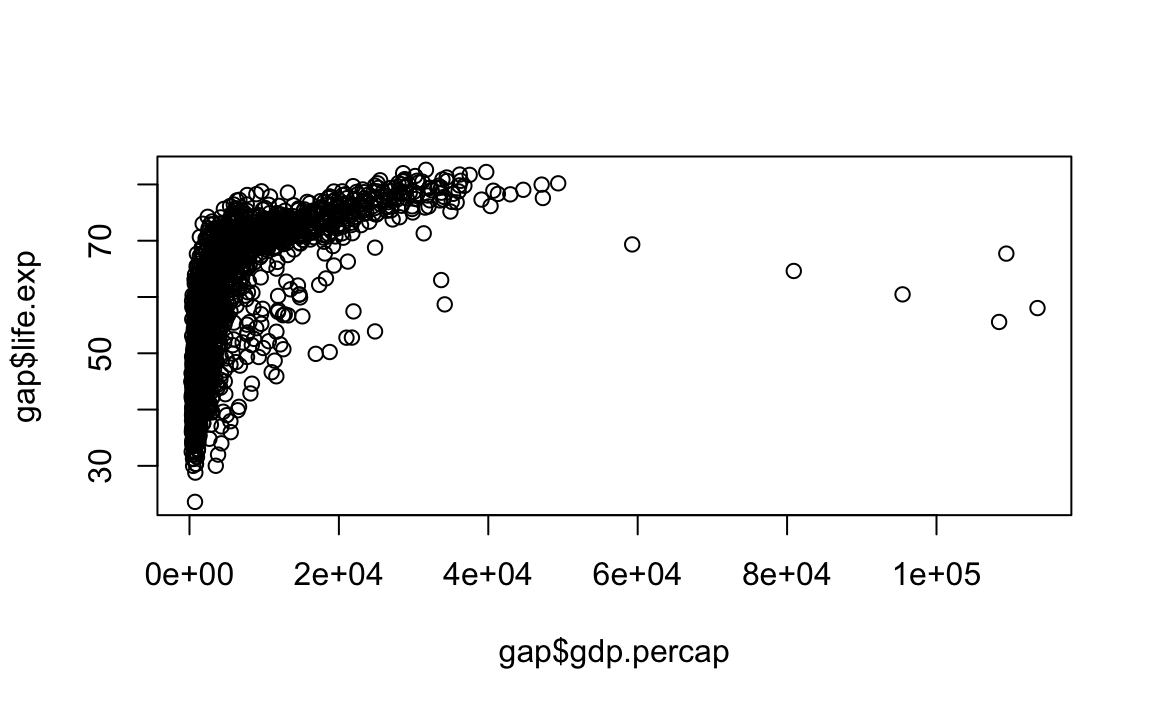
\includegraphics[width=0.7\linewidth]{site1_files/figure-latex/unnamed-chunk-205-1} \end{center}

Finally, let's quickly take a look at a histogram of the variable
\texttt{nyt.count}:

\begin{Shaded}
\begin{Highlighting}[]
\KeywordTok{hist}\NormalTok{(gap}\OperatorTok{$}\NormalTok{life.exp, }\DataTypeTok{breaks =} \DecValTok{100}\NormalTok{)}
\end{Highlighting}
\end{Shaded}

\begin{center}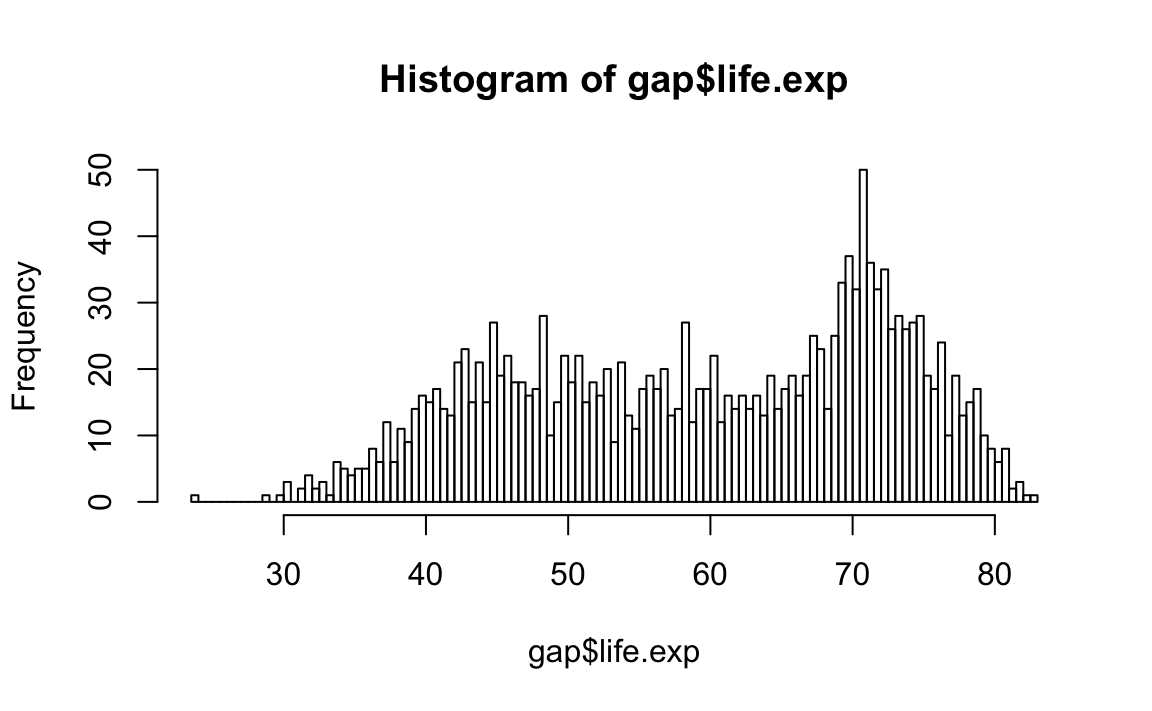
\includegraphics[width=0.7\linewidth]{site1_files/figure-latex/unnamed-chunk-206-1} \end{center}

\subsection{Challenges}\label{challenges-10}

\begin{enumerate}
\def\labelenumi{\arabic{enumi})}
\item
  Read the \texttt{polity} dataset.
\item
  Report the number and names of each variable in the dataset.
\item
  Extract the 5th row from the polity dataset.
\item
  Extract the last row from the polity dataset.
\item
  Count the percentage of obesrvations with a value of \texttt{polity2}
  greater than 8 in the gapminder dataset (hint: if using sum(), read
  the help file..
\item
  Set all of the values of \texttt{democ} and \texttt{autac} columns
  less than -10 to NA. (Hint: You should first copy the \texttt{polity}
  object and work on the copy so that the original dataset is unchanged
  (or just read the data into R again afterwards to get a clean copy).
\end{enumerate}

\chapter{Data transformation}\label{data-transformation}

\section{Introduction}\label{introduction}

\subsection{\texorpdfstring{\texttt{tidyverse}}{tidyverse}}\label{tidyverse}

\begin{quote}
It is often said that 80\% of data analysis is spent on the process of
cleaning and preparing the data. (Dasu and Johnson, 2003)
\end{quote}

For most applied researchers, data preparation usually involves 3 main
steps.

\begin{enumerate}
\def\labelenumi{\arabic{enumi}.}
\tightlist
\item
  \textbf{\emph{Transforming}} data frames, e.g.~filtering, summarizing,
  and conducting calculations across groups.
\item
  \textbf{\emph{Tidying}} data into the appropriate format.
\item
  \textbf{\emph{Merging}} or linking several datasets to create a bigger
  dataset.
\end{enumerate}

The \href{https://www.tidyverse.org/}{\texttt{tidyverse}} is a suite of
packages designed specifically to help with these steps. These are by no
means the only packages out there for data wrangling but they are
increasingly popular for their readable, straightforward syntax and
sensible default behaviors.

In this chapter we're going to focus on how to use the \texttt{dplyr}
package for data transformation tasks.

\subsection{Gapminder}\label{gapminder}

For this unit, we'll be working with the ``Gapminder'' dataset, which is
excerpt of the data available at Gapminder.org. For each of 142
countries, the data provides values for life expectancy, GDP per capita,
and population, every five years, from 1952 to 2007.

\begin{Shaded}
\begin{Highlighting}[]
\NormalTok{gap <-}\StringTok{ }\KeywordTok{read.csv}\NormalTok{(}\StringTok{"data/gapminder-FiveYearData.csv"}\NormalTok{, }\DataTypeTok{stringsAsFactors =} \OtherTok{TRUE}\NormalTok{)}
\KeywordTok{kable}\NormalTok{(}\KeywordTok{head}\NormalTok{(gap))}
\end{Highlighting}
\end{Shaded}

country

year

pop

continent

lifeExp

gdpPercap

Afghanistan

1952

8425333

Asia

28.8

779

Afghanistan

1957

9240934

Asia

30.3

821

Afghanistan

1962

10267083

Asia

32.0

853

Afghanistan

1967

11537966

Asia

34.0

836

Afghanistan

1972

13079460

Asia

36.1

740

Afghanistan

1977

14880372

Asia

38.4

786

\subsection{\texorpdfstring{why
\texttt{dplyr}?}{why dplyr?}}\label{why-dplyr}

So far, you've seen the basics of manipulating data frames,
e.g.~subsetting and basic calculations. For instance, we can use base R
functions to calculate summary statistics across groups of observations,
e.g., the mean GDP per capita within each region:

\begin{Shaded}
\begin{Highlighting}[]
\KeywordTok{mean}\NormalTok{(gap[gap}\OperatorTok{$}\NormalTok{continent }\OperatorTok{==}\StringTok{ "Africa"}\NormalTok{, }\StringTok{"gdpPercap"}\NormalTok{])}
\CommentTok{#> [1] 2194}
\KeywordTok{mean}\NormalTok{(gap[gap}\OperatorTok{$}\NormalTok{continent }\OperatorTok{==}\StringTok{ "Americas"}\NormalTok{, }\StringTok{"gdpPercap"}\NormalTok{])}
\CommentTok{#> [1] 7136}
\KeywordTok{mean}\NormalTok{(gap[gap}\OperatorTok{$}\NormalTok{continent }\OperatorTok{==}\StringTok{ "Asia"}\NormalTok{, }\StringTok{"gdpPercap"}\NormalTok{])}
\CommentTok{#> [1] 7902}
\end{Highlighting}
\end{Shaded}

But this isn't ideal because it involves a fair bit of repetition.
Repeating yourself will cost you time, both now and later, and
potentially introduce some nasty bugs.

Luckily, the
\href{https://cran.r-project.org/web/packages/dplyr/dplyr.pdf}{\texttt{dplyr}}
package provides a number of very useful functions for manipulating
dataframes. These functions will save you time by reducing repetition.
As an added bonus, you might even find the \texttt{dplyr} grammar easier
to read.

Here we're going to cover 6 of the most commonly used functions as well
as using pipes (\texttt{\%\textgreater{}\%}) to combine them.

\begin{enumerate}
\def\labelenumi{\arabic{enumi}.}
\tightlist
\item
  \texttt{select()}
\item
  \texttt{filter()}
\item
  \texttt{group\_by()}
\item
  \texttt{summarize()}
\item
  \texttt{mutate()}
\item
  \texttt{arrange()}
\end{enumerate}

If you have have not installed this package earlier, please do so now:

\begin{Shaded}
\begin{Highlighting}[]
\CommentTok{# not run}
\CommentTok{# install.packages('dplyr')}
\end{Highlighting}
\end{Shaded}

Now let's load the package:

\begin{Shaded}
\begin{Highlighting}[]
\KeywordTok{library}\NormalTok{(dplyr)}
\end{Highlighting}
\end{Shaded}

\section{\texorpdfstring{\texttt{dplyr}
functions}{dplyr functions}}\label{dplyr-functions}

\subsection{\texorpdfstring{Select columns with
\texttt{select}}{Select columns with select}}\label{select-columns-with-select}

Imagine that we just received the gapminder dataset, but are only
interested in a few variables in it. We could use the \texttt{select()}
function to keep only the variables we select.

\begin{Shaded}
\begin{Highlighting}[]
\NormalTok{year_country_gdp <-}\StringTok{ }\KeywordTok{select}\NormalTok{(gap, year, country, gdpPercap)}
\KeywordTok{kable}\NormalTok{(}\KeywordTok{head}\NormalTok{(year_country_gdp))}
\end{Highlighting}
\end{Shaded}

year

country

gdpPercap

1952

Afghanistan

779

1957

Afghanistan

821

1962

Afghanistan

853

1967

Afghanistan

836

1972

Afghanistan

740

1977

Afghanistan

786

\begin{Shaded}
\begin{Highlighting}[]
\NormalTok{knitr}\OperatorTok{::}\KeywordTok{include_graphics}\NormalTok{(}\DataTypeTok{path =} \StringTok{"img/dplyr-fig1.png"}\NormalTok{)}
\end{Highlighting}
\end{Shaded}

\begin{center}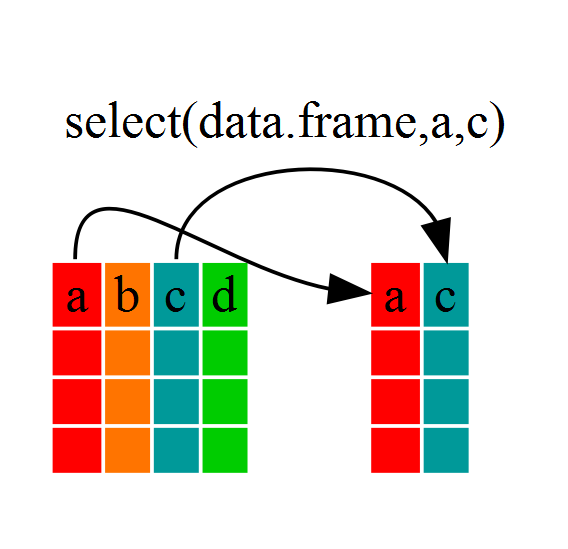
\includegraphics[width=0.7\linewidth]{img/dplyr-fig1} \end{center}

If we open up \texttt{year\_country\_gdp}, we'll see that it only
contains the year, country and gdpPercap. This is equivalent to the base
R subsetting function:

\begin{Shaded}
\begin{Highlighting}[]
\NormalTok{year_country_gdp_base <-}\StringTok{ }\NormalTok{gap[,}\KeywordTok{c}\NormalTok{(}\StringTok{"year"}\NormalTok{, }\StringTok{"country"}\NormalTok{, }\StringTok{"gdpPercap"}\NormalTok{)]}
\KeywordTok{kable}\NormalTok{(}\KeywordTok{head}\NormalTok{(year_country_gdp))}
\end{Highlighting}
\end{Shaded}

year

country

gdpPercap

1952

Afghanistan

779

1957

Afghanistan

821

1962

Afghanistan

853

1967

Afghanistan

836

1972

Afghanistan

740

1977

Afghanistan

786

But, as we will see, \texttt{dplyr} makes for much more readible,
efficient code because of its \emph{pipe} operator.

\subsection{The pipe}\label{the-pipe}

\begin{Shaded}
\begin{Highlighting}[]
\NormalTok{knitr}\OperatorTok{::}\KeywordTok{include_graphics}\NormalTok{(}\DataTypeTok{path =} \StringTok{"img/pipe.jpg"}\NormalTok{)}
\end{Highlighting}
\end{Shaded}

\begin{center}
\includegraphics[width=0.7\linewidth]{img/pipe} \end{center}

Above, we used what's called `normal' grammar, but the strengths of
\texttt{dplyr} lie in combining several functions using \emph{pipes}.
Since the pipes grammar is unlike anything we've seen in R before, let's
repeat what we've done above using pipes.

Above, we used what's called ``normal'' grammar, but the strengths of
\texttt{dplyr} lie in combining several functions using \emph{pipes}.

In typical base R code, a simple operation might be written like:

\begin{Shaded}
\begin{Highlighting}[]
\CommentTok{# NOT run}
\NormalTok{cupcakes <-}\StringTok{ }\KeywordTok{bake}\NormalTok{(}\KeywordTok{pour}\NormalTok{(}\KeywordTok{mix}\NormalTok{(ingredients)))}
\end{Highlighting}
\end{Shaded}

A computer has no trouble understanding this and your cupcakes will be
made just fine but a person has to read right to left to understand the
order of operations - the opposite of how most western languages are
read - making it harder to understand what is being done!

To be more readable without pipes, we might break up this code into
intermediate objects\ldots{}

\begin{Shaded}
\begin{Highlighting}[]
\NormalTok{## NOT run}
\NormalTok{batter <-}\StringTok{ }\KeywordTok{mix}\NormalTok{(ingredients)}
\NormalTok{muffin_tin <-}\StringTok{ }\KeywordTok{pour}\NormalTok{(batter)}
\NormalTok{cupcakes <-}\StringTok{ }\KeywordTok{bake}\NormalTok{(muffin_tin)}
\end{Highlighting}
\end{Shaded}

but this can clutter our environment with a lot of variables that aren't
very useful to us, and often are named very similar things (e.g.~step,
step1, step2\ldots{}) which can lead to confusion and those
hard-to-track-down bugs.

\subsubsection*{Enter the pipe\ldots{}}\label{enter-the-pipe}
\addcontentsline{toc}{subsubsection}{Enter the pipe\ldots{}}

The \emph{pipe} makes it easier to read code because it lays out the
operations left to right so each line can be read like a line of a
recipe for the perfect data frame!

Pipes take the input on the left side of the \texttt{\%\textgreater{}\%}
symbol and pass it in as the first argument to the function on the right
side.

With pipes, our cupcake example might be written like:

\begin{Shaded}
\begin{Highlighting}[]
\NormalTok{## NOT run}
\NormalTok{cupcakes <-}\StringTok{ }\NormalTok{ingredients }\OperatorTok\StringTok{ }
\StringTok{  }\KeywordTok{mix}\NormalTok{() }\OperatorTok\StringTok{ }
\StringTok{  }\KeywordTok{pour}\NormalTok{() }\OperatorTok\StringTok{ }
\StringTok{  }\KeywordTok{bake}\NormalTok{()}
\end{Highlighting}
\end{Shaded}

\subsubsection*{Tips for piping}\label{tips-for-piping}
\addcontentsline{toc}{subsubsection}{Tips for piping}

\begin{enumerate}
\def\labelenumi{\arabic{enumi}.}
\item
  Remember though that you don't assign anything within the pipes - that
  is, you should not use \textless{}- inside the piped operation. Only
  use this at the beginning if you want to save the output.
\item
  Remember to add the pipe \texttt{\%\textgreater{}\%} at the end of
  each line involved in the piped operation. A good rule of thumb:
  RStudio will automatically indent lines of code that are part of a
  piped operation. If the line isn't indented, it probably hasn't been
  added to the pipe. If you have an error in a piped operation, always
  check to make sure the pipe is connected as you expect.
\item
  In RStudio the hotkey for the pipe is Ctrl + Shift + M.
\end{enumerate}

\subsubsection*{\texorpdfstring{\texttt{select} \& Pipe
(\texttt{\%\textgreater{}\%})}{select \& Pipe (\%\textgreater{}\%)}}\label{select-pipe}
\addcontentsline{toc}{subsubsection}{\texttt{select} \& Pipe
(\texttt{\%\textgreater{}\%})}

Since the pipe grammar is unlike anything we've seen in R before, let's
repeat what we did above with the gapminder dataset using pipes:

\begin{Shaded}
\begin{Highlighting}[]
\NormalTok{year_country_gdp <-}\StringTok{ }\NormalTok{gap }\OperatorTok\StringTok{ }\KeywordTok{select}\NormalTok{(year, country, gdpPercap)}
\end{Highlighting}
\end{Shaded}

Let's walk through it step by step. First, we summon the gapminder data
frame and pass it on to the next step using the pipe symbol
\texttt{\%\textgreater{}\%}. The second step is the \texttt{select()}
function. In this case we don't specify which data object we use in the
call to \texttt{select()} since we've piped it in.

\textbf{Fun Fact}: There is a good chance you have encountered pipes
before in the shell. In R, a pipe symbol is \texttt{\%\textgreater{}\%}
while in the shell it is \texttt{\textbar{}.} But the concept is the
same!

\subsection{\texorpdfstring{Filter rows with
\texttt{filter}}{Filter rows with filter}}\label{filter-rows-with-filter}

Now let's say we're only interested in African countries. We can combine
\texttt{select} and \texttt{filter} to select only the observations
where \texttt{continent} is \texttt{Africa}.

\begin{Shaded}
\begin{Highlighting}[]
\NormalTok{year_country_gdp_africa <-}\StringTok{ }\NormalTok{gap }\OperatorTok
\StringTok{    }\KeywordTok{filter}\NormalTok{(continent }\OperatorTok{==}\StringTok{ "Africa"}\NormalTok{) }\OperatorTok
\StringTok{    }\KeywordTok{select}\NormalTok{(year, country, gdpPercap)}
\end{Highlighting}
\end{Shaded}

As with last time, first we pass the gapminder dataframe to the
\texttt{filter()} function, then we pass the filtered version of the
gapminder dataframe to the \texttt{select()} function.

To clarify, both the \texttt{select} and \texttt{filter} functions
subsets the data frame. The difference is that \texttt{select} extracts
certain columns, while \texttt{filter} extracts certain rows.

\textbf{Note:} The order of operations is very important in this case.
If we used \texttt{select} first, filter would not be able to find the
variable \texttt{continent} since we would have removed it in the
previous step.

\subsection{\texorpdfstring{Calculate across groups with
\texttt{group\_by}}{Calculate across groups with group\_by}}\label{calculate-across-groups-with-group_by}

A common task you'll encounter when working with data is running
calculations on different groups within the data. For instance, what if
we wanted to calculated the mean GDP per capita for each continent?

In base R, you would have to run the \texttt{mean()} function for each
subset of data:

\begin{Shaded}
\begin{Highlighting}[]
\KeywordTok{mean}\NormalTok{(gap}\OperatorTok{$}\NormalTok{gdpPercap[gap}\OperatorTok{$}\NormalTok{continent }\OperatorTok{==}\StringTok{ "Africa"}\NormalTok{])}
\CommentTok{#> [1] 2194}
\KeywordTok{mean}\NormalTok{(gap}\OperatorTok{$}\NormalTok{gdpPercap[gap}\OperatorTok{$}\NormalTok{continent }\OperatorTok{==}\StringTok{ "Americas"}\NormalTok{])}
\CommentTok{#> [1] 7136}
\KeywordTok{mean}\NormalTok{(gap}\OperatorTok{$}\NormalTok{gdpPercap[gap}\OperatorTok{$}\NormalTok{continent }\OperatorTok{==}\StringTok{ "Asia"}\NormalTok{])}
\CommentTok{#> [1] 7902}
\KeywordTok{mean}\NormalTok{(gap}\OperatorTok{$}\NormalTok{gdpPercap[gap}\OperatorTok{$}\NormalTok{continent }\OperatorTok{==}\StringTok{ "Europe"}\NormalTok{])}
\CommentTok{#> [1] 14469}
\KeywordTok{mean}\NormalTok{(gap}\OperatorTok{$}\NormalTok{gdpPercap[gap}\OperatorTok{$}\NormalTok{continent }\OperatorTok{==}\StringTok{ "Oceania"}\NormalTok{])}
\CommentTok{#> [1] 18622}
\end{Highlighting}
\end{Shaded}

That's a lot of repetition! To make matters worse, what if we wanted to
add these values to our original data frame as a new column? We would
have to write something like this:

\begin{Shaded}
\begin{Highlighting}[]
\NormalTok{gap}\OperatorTok{$}\NormalTok{mean.continent.GDP <-}\StringTok{ }\OtherTok{NA}
\NormalTok{gap}\OperatorTok{$}\NormalTok{mean.continent.GDP[gap}\OperatorTok{$}\NormalTok{continent }\OperatorTok{==}\StringTok{ "Africa"}\NormalTok{] <-}\StringTok{ }\KeywordTok{mean}\NormalTok{(gap}\OperatorTok{$}\NormalTok{gdpPercap[gap}\OperatorTok{$}\NormalTok{continent }\OperatorTok{==}\StringTok{ "Africa"}\NormalTok{])}
\NormalTok{gap}\OperatorTok{$}\NormalTok{mean.continent.GDP[gap}\OperatorTok{$}\NormalTok{continent }\OperatorTok{==}\StringTok{ "Americas"}\NormalTok{] <-}\StringTok{ }\KeywordTok{mean}\NormalTok{(gap}\OperatorTok{$}\NormalTok{gdpPercap[gap}\OperatorTok{$}\NormalTok{continent }\OperatorTok{==}\StringTok{ "Americas"}\NormalTok{])}
\NormalTok{gap}\OperatorTok{$}\NormalTok{mean.continent.GDP[gap}\OperatorTok{$}\NormalTok{continent }\OperatorTok{==}\StringTok{ "Asia"}\NormalTok{] <-}\StringTok{ }\KeywordTok{mean}\NormalTok{(gap}\OperatorTok{$}\NormalTok{gdpPercap[gap}\OperatorTok{$}\NormalTok{continent }\OperatorTok{==}\StringTok{ "Asia"}\NormalTok{])}
\NormalTok{gap}\OperatorTok{$}\NormalTok{mean.continent.GDP[gap}\OperatorTok{$}\NormalTok{continent }\OperatorTok{==}\StringTok{ "Europe"}\NormalTok{] <-}\StringTok{ }\KeywordTok{mean}\NormalTok{(gap}\OperatorTok{$}\NormalTok{gdpPercap[gap}\OperatorTok{$}\NormalTok{continent }\OperatorTok{==}\StringTok{ "Europe"}\NormalTok{])}
\NormalTok{gap}\OperatorTok{$}\NormalTok{mean.continent.GDP[gap}\OperatorTok{$}\NormalTok{continent }\OperatorTok{==}\StringTok{ "Oceania"}\NormalTok{] <-}\StringTok{ }\KeywordTok{mean}\NormalTok{(gap}\OperatorTok{$}\NormalTok{gdpPercap[gap}\OperatorTok{$}\NormalTok{continent }\OperatorTok{==}\StringTok{ "Oceania"}\NormalTok{])}
\end{Highlighting}
\end{Shaded}

You can see how this can get pretty tedious, especially if we want to
calculate more complicated or refined statistics. We could use loops or
apply functions, but these can be difficult, slow, or error-prone.

\subsubsection*{split-apply-combine}\label{split-apply-combine}
\addcontentsline{toc}{subsubsection}{split-apply-combine}

The abstract problem we're encountering here is know as
``split-apply-combine'':

\begin{Shaded}
\begin{Highlighting}[]
\NormalTok{knitr}\OperatorTok{::}\KeywordTok{include_graphics}\NormalTok{(}\DataTypeTok{path =} \StringTok{"img/splitapply.png"}\NormalTok{)}
\end{Highlighting}
\end{Shaded}

\begin{center}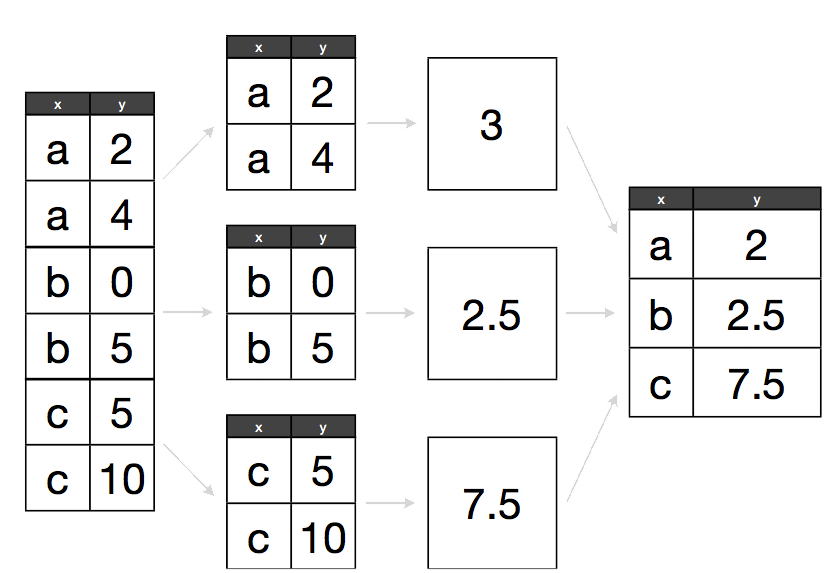
\includegraphics[width=0.7\linewidth]{img/splitapply} \end{center}

We want to \emph{split} our data into groups (in this case continents),
\emph{apply} some calculations on that group, then \emph{combine} the
results together afterwards.

Luckily, \texttt{dplyr} offers a much cleaner, straight-forward solution
to this problem.

First, let's remove the column we just made.

\begin{Shaded}
\begin{Highlighting}[]
\NormalTok{gap <-}\StringTok{ }\NormalTok{gap }\OperatorTok\StringTok{ }\KeywordTok{select}\NormalTok{(}\OperatorTok{-}\NormalTok{mean.continent.GDP) }\CommentTok{# drop a column with - }
\CommentTok{# OR}
\NormalTok{gap}\OperatorTok{$}\NormalTok{mean.continent.GDP <-}\StringTok{ }\OtherTok{NULL}
\end{Highlighting}
\end{Shaded}

\subsubsection{\texorpdfstring{\texttt{group\_by}}{group\_by}}\label{group_by}

We've already seen how \texttt{filter()} can help us select observations
that meet certain criteria (in the above:
\texttt{continent\ ==\ "Africa"}). More helpful, however, is the
\texttt{group\_by()} function, which will essentially use every unique
criteria that we could have used in \texttt{filter()}.

A \texttt{grouped\_df} can be thought of as a \texttt{list} where each
item in the \texttt{list} is a \texttt{data.frame} which contains only
the rows that correspond to the a particular value \texttt{continent}
(at least in the example above).

\begin{Shaded}
\begin{Highlighting}[]
\NormalTok{knitr}\OperatorTok{::}\KeywordTok{include_graphics}\NormalTok{(}\DataTypeTok{path =} \StringTok{"img/dplyr-fig2.png"}\NormalTok{)}
\end{Highlighting}
\end{Shaded}

\begin{center}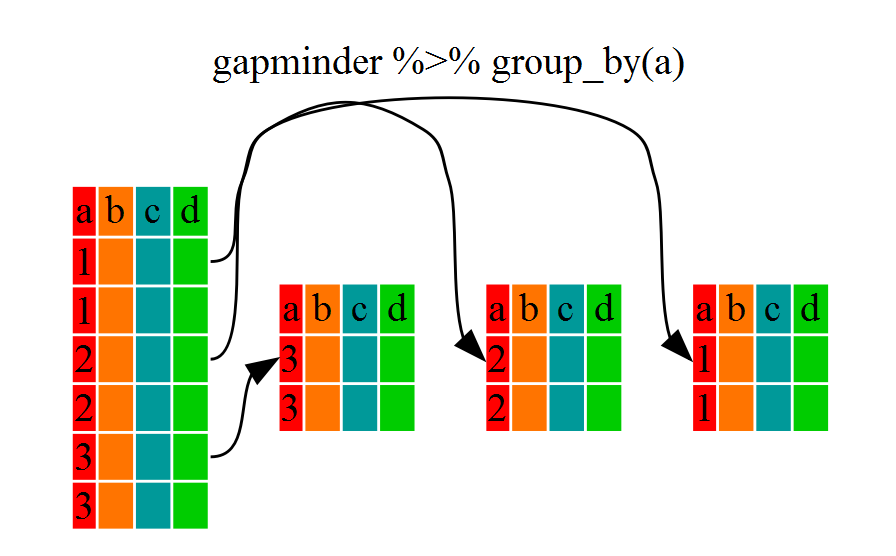
\includegraphics[width=0.7\linewidth]{img/dplyr-fig2} \end{center}

\subsection{\texorpdfstring{Summerarize across groups with
\texttt{summarize}}{Summerarize across groups with summarize}}\label{summerarize-across-groups-with-summarize}

\texttt{group\_by()} on its own is not particularly interesting. It's
much more exciting used in conjunction with the \texttt{summarize()}
function.

This will allow use to create new variable(s) by applying
transformations to variables in each of the continent-specific data
frames.

In other words, using the \texttt{group\_by()} function, we split our
original data frame into multipl pieces, which we then apply summary
functions to (e.g. \texttt{mean()} or \texttt{sd()}) within
\texttt{summarize()}.

The output is a new data frame reduced in size, with one row per group.

\begin{Shaded}
\begin{Highlighting}[]
\NormalTok{gdp_bycontinents <-}\StringTok{ }\NormalTok{gap }\OperatorTok
\StringTok{    }\KeywordTok{group_by}\NormalTok{(continent) }\OperatorTok
\StringTok{    }\KeywordTok{summarize}\NormalTok{(}\DataTypeTok{mean_gdpPercap =} \KeywordTok{mean}\NormalTok{(gdpPercap))}
\KeywordTok{kable}\NormalTok{(}\KeywordTok{head}\NormalTok{(gdp_bycontinents))}
\end{Highlighting}
\end{Shaded}

continent

mean\_gdpPercap

Africa

2194

Americas

7136

Asia

7902

Europe

14469

Oceania

18622

\begin{Shaded}
\begin{Highlighting}[]
\NormalTok{knitr}\OperatorTok{::}\KeywordTok{include_graphics}\NormalTok{(}\DataTypeTok{path =} \StringTok{"img/dplyr-fig3.png"}\NormalTok{)}
\end{Highlighting}
\end{Shaded}

\begin{center}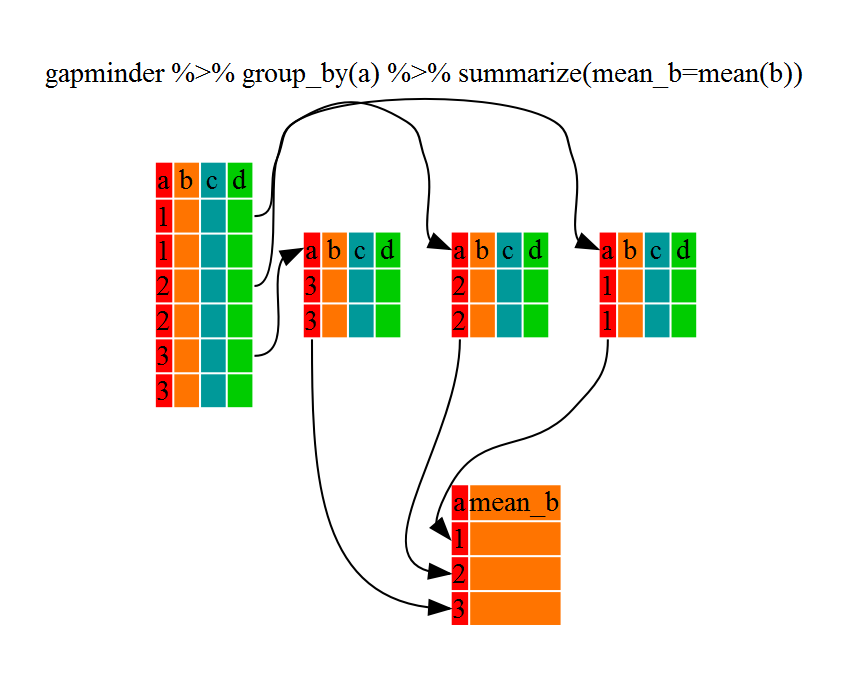
\includegraphics[width=0.7\linewidth]{img/dplyr-fig3} \end{center}

That allowed us to calculate the mean gdpPercap for each continent.

But it gets even better -- the function \texttt{group\_by()} allows us
to group by multiple variables. Let's group by \texttt{year} and
\texttt{continent}.

\begin{Shaded}
\begin{Highlighting}[]
\NormalTok{gdp_bycontinents_byyear <-}\StringTok{ }\NormalTok{gap }\OperatorTok
\StringTok{    }\KeywordTok{group_by}\NormalTok{(continent, year) }\OperatorTok
\StringTok{    }\KeywordTok{summarize}\NormalTok{(}\DataTypeTok{mean_gdpPercap =} \KeywordTok{mean}\NormalTok{(gdpPercap))}
\KeywordTok{kable}\NormalTok{(}\KeywordTok{head}\NormalTok{(gdp_bycontinents_byyear))}
\end{Highlighting}
\end{Shaded}

continent

year

mean\_gdpPercap

Africa

1952

1253

Africa

1957

1385

Africa

1962

1598

Africa

1967

2050

Africa

1972

2340

Africa

1977

2586

That is already quite powerful, but it gets even better! You're not
limited to defining 1 new variable in \texttt{summarize()}.

\begin{Shaded}
\begin{Highlighting}[]
\NormalTok{gdp_pop_bycontinents_byyear <-}\StringTok{ }\NormalTok{gap }\OperatorTok
\StringTok{    }\KeywordTok{group_by}\NormalTok{(continent, year) }\OperatorTok
\StringTok{    }\KeywordTok{summarize}\NormalTok{(}\DataTypeTok{mean_gdpPercap =} \KeywordTok{mean}\NormalTok{(gdpPercap),}
              \DataTypeTok{sd_gdpPercap =} \KeywordTok{sd}\NormalTok{(gdpPercap),}
              \DataTypeTok{mean_pop =} \KeywordTok{mean}\NormalTok{(pop),}
              \DataTypeTok{sd_pop =} \KeywordTok{sd}\NormalTok{(pop))}
\KeywordTok{kable}\NormalTok{(}\KeywordTok{head}\NormalTok{(gdp_pop_bycontinents_byyear))}
\end{Highlighting}
\end{Shaded}

continent

year

mean\_gdpPercap

sd\_gdpPercap

mean\_pop

sd\_pop

Africa

1952

1253

983

4570010

6317450

Africa

1957

1385

1135

5093033

7076042

Africa

1962

1598

1462

5702247

7957545

Africa

1967

2050

2848

6447875

8985505

Africa

1972

2340

3287

7305376

10130833

Africa

1977

2586

4142

8328097

11585184

\subsection{\texorpdfstring{Add new variables with
\texttt{mutate}}{Add new variables with mutate}}\label{add-new-variables-with-mutate}

What if we wanted to add these values to our original data frame instead
of creating a new object?

For this, we can use the \texttt{mutate()} function, which is similar to
\texttt{summarize()} except it creates new variables to the same
dataframe that you pass into it.

\begin{Shaded}
\begin{Highlighting}[]
\NormalTok{gapminder_with_extra_vars <-}\StringTok{ }\NormalTok{gap }\OperatorTok
\StringTok{    }\KeywordTok{group_by}\NormalTok{(continent, year) }\OperatorTok
\StringTok{    }\KeywordTok{mutate}\NormalTok{(}\DataTypeTok{mean_gdpPercap =} \KeywordTok{mean}\NormalTok{(gdpPercap),}
              \DataTypeTok{sd_gdpPercap =} \KeywordTok{sd}\NormalTok{(gdpPercap),}
              \DataTypeTok{mean_pop =} \KeywordTok{mean}\NormalTok{(pop),}
              \DataTypeTok{sd_pop =} \KeywordTok{sd}\NormalTok{(pop))}
\KeywordTok{kable}\NormalTok{(}\KeywordTok{head}\NormalTok{(gapminder_with_extra_vars))}
\end{Highlighting}
\end{Shaded}

country

year

pop

continent

lifeExp

gdpPercap

mean\_gdpPercap

sd\_gdpPercap

mean\_pop

sd\_pop

Afghanistan

1952

8425333

Asia

28.8

779

5195

18635

42283556

1.13e+08

Afghanistan

1957

9240934

Asia

30.3

821

5788

19507

47356988

1.28e+08

Afghanistan

1962

10267083

Asia

32.0

853

5729

16416

51404763

1.36e+08

Afghanistan

1967

11537966

Asia

34.0

836

5971

14063

57747361

1.53e+08

Afghanistan

1972

13079460

Asia

36.1

740

8187

19088

65180977

1.74e+08

Afghanistan

1977

14880372

Asia

38.4

786

7791

11816

72257987

1.92e+08

We can use also use \texttt{mutate()} to create new variables prior to
(or even after) summarizing information.

\begin{Shaded}
\begin{Highlighting}[]
\NormalTok{gdp_pop_bycontinents_byyear <-}\StringTok{ }\NormalTok{gap }\OperatorTok
\StringTok{    }\KeywordTok{mutate}\NormalTok{(}\DataTypeTok{gdp_billion =}\NormalTok{ gdpPercap}\OperatorTok{*}\NormalTok{pop}\OperatorTok{/}\DecValTok{10}\OperatorTok{^}\DecValTok{9}\NormalTok{) }\OperatorTok
\StringTok{    }\KeywordTok{group_by}\NormalTok{(continent, year) }\OperatorTok
\StringTok{    }\KeywordTok{summarize}\NormalTok{(}\DataTypeTok{mean_gdpPercap =} \KeywordTok{mean}\NormalTok{(gdpPercap),}
              \DataTypeTok{sd_gdpPercap =} \KeywordTok{sd}\NormalTok{(gdpPercap),}
              \DataTypeTok{mean_pop =} \KeywordTok{mean}\NormalTok{(pop),}
              \DataTypeTok{sd_pop =} \KeywordTok{sd}\NormalTok{(pop),}
              \DataTypeTok{mean_gdp_billion =} \KeywordTok{mean}\NormalTok{(gdp_billion),}
              \DataTypeTok{sd_gdp_billion =} \KeywordTok{sd}\NormalTok{(gdp_billion))}
\KeywordTok{kable}\NormalTok{(}\KeywordTok{head}\NormalTok{(gdp_pop_bycontinents_byyear))}
\end{Highlighting}
\end{Shaded}

continent

year

mean\_gdpPercap

sd\_gdpPercap

mean\_pop

sd\_pop

mean\_gdp\_billion

sd\_gdp\_billion

Africa

1952

1253

983

4570010

6317450

5.99

11.4

Africa

1957

1385

1135

5093033

7076042

7.36

14.5

Africa

1962

1598

1462

5702247

7957545

8.79

17.2

Africa

1967

2050

2848

6447875

8985505

11.44

23.2

Africa

1972

2340

3287

7305376

10130833

15.07

30.4

Africa

1977

2586

4142

8328097

11585184

18.70

38.1

\subsubsection*{\texorpdfstring{\texttt{mutate} vs.
\texttt{summarize}}{mutate vs. summarize}}\label{mutate-vs.-summarize}
\addcontentsline{toc}{subsubsection}{\texttt{mutate} vs.
\texttt{summarize}}

It can be confusing to decide whether to use \texttt{mutate} or
\texttt{summarize}. The key distinction is whether you want the output
to have one row for each group or one row for each row in the original
data frame:

\begin{itemize}
\tightlist
\item
  \texttt{mutate}: creates new columns with as many rows as the original
  data frame
\item
  \texttt{summarize}: creates a data frame with as many rows as groups
\end{itemize}

Note that if you use an aggregation function such as \texttt{mean()}
within \texttt{mutate()} without using \texttt{groupby()}, you'll simply
do the summary over all the rows of the input data frame.

And if you use an aggregation function such as \texttt{mean()} within
\texttt{summarize()} without using \texttt{groupby()}, you'll simply
create an output data frame with one row (i.e., the whole input data
frame is a single group).

\subsection{\texorpdfstring{Arrange rows with
\texttt{arrange}}{Arrange rows with arrange}}\label{arrange-rows-with-arrange}

As a last step, let's say we want to sort the rows in our data frame
according to values in a certain column. We can use the
\texttt{arrange()} function to do this. For instance, let's organize our
rows by \texttt{year} (recent first), and then by \texttt{continent}.

\begin{Shaded}
\begin{Highlighting}[]
\NormalTok{gapminder_with_extra_vars <-}\StringTok{ }\NormalTok{gap }\OperatorTok
\StringTok{    }\KeywordTok{group_by}\NormalTok{(continent, year) }\OperatorTok
\StringTok{    }\KeywordTok{mutate}\NormalTok{(}\DataTypeTok{mean_gdpPercap =} \KeywordTok{mean}\NormalTok{(gdpPercap),}
              \DataTypeTok{sd_gdpPercap =} \KeywordTok{sd}\NormalTok{(gdpPercap),}
              \DataTypeTok{mean_pop =} \KeywordTok{mean}\NormalTok{(pop),}
              \DataTypeTok{sd_pop =} \KeywordTok{sd}\NormalTok{(pop)) }\OperatorTok
\StringTok{    }\KeywordTok{arrange}\NormalTok{(}\KeywordTok{desc}\NormalTok{(year), continent)}
\KeywordTok{kable}\NormalTok{(}\KeywordTok{head}\NormalTok{(gapminder_with_extra_vars))}
\end{Highlighting}
\end{Shaded}

country

year

pop

continent

lifeExp

gdpPercap

mean\_gdpPercap

sd\_gdpPercap

mean\_pop

sd\_pop

Algeria

2007

33333216

Africa

72.3

6223

3089

3618

17875763

24917726

Angola

2007

12420476

Africa

42.7

4797

3089

3618

17875763

24917726

Benin

2007

8078314

Africa

56.7

1441

3089

3618

17875763

24917726

Botswana

2007

1639131

Africa

50.7

12570

3089

3618

17875763

24917726

Burkina Faso

2007

14326203

Africa

52.3

1217

3089

3618

17875763

24917726

Burundi

2007

8390505

Africa

49.6

430

3089

3618

17875763

24917726

\section{\texorpdfstring{\texttt{dplyr} and ``non-standard
evaluation''}{dplyr and non-standard evaluation}}\label{dplyr-and-non-standard-evaluation}

You may run across the term ``non-standard evaluation''. The use of data
frame variables without quotes around them is an example of this.

Why is this strange?

\begin{Shaded}
\begin{Highlighting}[]
\NormalTok{gap }\OperatorTok\StringTok{ }\KeywordTok{select}\NormalTok{(continent, year) }\OperatorTok\StringTok{ }\KeywordTok{tail}\NormalTok{()}
\end{Highlighting}
\end{Shaded}

Compare it to:

\begin{Shaded}
\begin{Highlighting}[]
\NormalTok{gap[ , }\KeywordTok{c}\NormalTok{(}\StringTok{'continent'}\NormalTok{, }\StringTok{'year'}\NormalTok{)]}
\NormalTok{gap[ , continent]}
\end{Highlighting}
\end{Shaded}

Because \texttt{continent} and \texttt{year} are not variables our
current environment! dplyr does some fancy stuff behind the scenes to
save us from typing the quotes.

This is fine if you have a data analysis workflow but if you want to
write a function that, for example, selects an arbitrary set of columns,
you'll run into trouble.

\begin{Shaded}
\begin{Highlighting}[]
\NormalTok{## here's a helper function that computes the mean of a variable, stratifying by a grouping variable}
\NormalTok{grouped_mean <-}\StringTok{ }\ControlFlowTok{function}\NormalTok{(data, group_var, summary_var) \{}
\NormalTok{  data }\OperatorTok
\StringTok{    }\KeywordTok{group_by}\NormalTok{(group_var) }\OperatorTok
\StringTok{    }\KeywordTok{summarise}\NormalTok{(}\DataTypeTok{mean =} \KeywordTok{mean}\NormalTok{(summary_var))}
\NormalTok{\}}
\NormalTok{gap }\OperatorTok\StringTok{ }\KeywordTok{grouped_mean}\NormalTok{(continent, lifeExp)}
\NormalTok{gap }\OperatorTok\StringTok{ }\KeywordTok{grouped_mean}\NormalTok{(}\StringTok{'continent'}\NormalTok{, }\StringTok{'lifeExp'}\NormalTok{)}
\end{Highlighting}
\end{Shaded}

See the \texttt{rlang} or \texttt{seplyr} packages for how one can deal
with this problem in this context of using functions.

\section{Challenges}\label{challenges-11}

\begin{enumerate}
\def\labelenumi{\arabic{enumi}.}
\item
  Use dplyr to create a data frame containing the median
  \texttt{lifeExp} for each continent
\item
  Use dplyr to add a column to the gapminder dataset that contains the
  total population of the continent of each observation in a given year.
  For example, if the first observation is Afghanistan in 1952, the new
  column would contain the population of Asia in 1952.
\item
  Use dplyr to: (a) add a column called \texttt{gdpPercap\_diff} that
  contains the difference between the observation's \texttt{gdpPercap}
  and the mean \texttt{gdpPercap} of the continent in that year, (b)
  arrange the dataframe by the column you just created, in descending
  order (so that the relatively richest country/years are listed first)
\end{enumerate}

\textbf{hint}: You might have to \texttt{ungoup()} before you
\texttt{arrange()}.

\subsubsection*{Acknowledgments}\label{acknowledgments-3}
\addcontentsline{toc}{subsubsection}{Acknowledgments}

Some of these materials in this module were adapted from:

\begin{itemize}
\tightlist
\item
  \href{http://swcarpentry.github.io/r-novice-gapminder/}{Software
  Carpentry})
\item
  \href{https://github.com/berkeley-scf/r-bootcamp-fall-2019}{R bootcamp
  at UC Berkeley}
\end{itemize}

\chapter{Tidying Data}\label{tidying-data}

Even before we conduct analysis or calculations, we need to put our data
into the correct format. The goal here is to rearrange a messy dataset
into one that is \textbf{tidy}

The two most important properties of tidy data are:

\begin{enumerate}
\def\labelenumi{\arabic{enumi})}
\tightlist
\item
  Each column is a variable.
\item
  Each row is an observation.
\end{enumerate}

Tidy data is easier to work with, because you have a consistent way of
referring to variables (as column names) and observations (as row
indices). It then becomes easy to manipulate, visualize, and model.

For more on the concept of \emph{tidy} data, read Hadley Wickham's paper
\href{http://vita.had.co.nz/papers/tidy-data.html}{here}

\section{Wide vs.~Long Formats}\label{wide-vs.long-formats}

\begin{quote}
``Tidy datasets are all alike but every messy dataset is messy in its
own way.'' -- Hadley Wickham
\end{quote}

Tabular datasets can be arranged in many ways. For instance, consider
the data below. Each data set displays information on heart rate
observed in individuals across 3 different time periods. But the data
are organized differently in each table.

\begin{Shaded}
\begin{Highlighting}[]
\NormalTok{wide <-}\StringTok{ }\KeywordTok{data.frame}\NormalTok{(}
  \DataTypeTok{name =} \KeywordTok{c}\NormalTok{(}\StringTok{"Wilbur"}\NormalTok{, }\StringTok{"Petunia"}\NormalTok{, }\StringTok{"Gregory"}\NormalTok{),}
  \DataTypeTok{time1 =} \KeywordTok{c}\NormalTok{(}\DecValTok{67}\NormalTok{, }\DecValTok{80}\NormalTok{, }\DecValTok{64}\NormalTok{),}
  \DataTypeTok{time2 =} \KeywordTok{c}\NormalTok{(}\DecValTok{56}\NormalTok{, }\DecValTok{90}\NormalTok{, }\DecValTok{50}\NormalTok{),}
  \DataTypeTok{time3 =} \KeywordTok{c}\NormalTok{(}\DecValTok{70}\NormalTok{, }\DecValTok{67}\NormalTok{, }\DecValTok{101}\NormalTok{)}
\NormalTok{)}
\KeywordTok{kable}\NormalTok{(wide)}
\end{Highlighting}
\end{Shaded}

name

time1

time2

time3

Wilbur

67

56

70

Petunia

80

90

67

Gregory

64

50

101

\begin{Shaded}
\begin{Highlighting}[]

\NormalTok{long <-}\StringTok{ }\KeywordTok{data.frame}\NormalTok{(}
  \DataTypeTok{name =} \KeywordTok{c}\NormalTok{(}\StringTok{"Wilbur"}\NormalTok{, }\StringTok{"Petunia"}\NormalTok{, }\StringTok{"Gregory"}\NormalTok{, }\StringTok{"Wilbur"}\NormalTok{, }\StringTok{"Petunia"}\NormalTok{, }\StringTok{"Gregory"}\NormalTok{, }\StringTok{"Wilbur"}\NormalTok{, }\StringTok{"Petunia"}\NormalTok{, }\StringTok{"Gregory"}\NormalTok{),}
  \DataTypeTok{time =} \KeywordTok{c}\NormalTok{(}\DecValTok{1}\NormalTok{, }\DecValTok{1}\NormalTok{, }\DecValTok{1}\NormalTok{, }\DecValTok{2}\NormalTok{, }\DecValTok{2}\NormalTok{, }\DecValTok{2}\NormalTok{, }\DecValTok{3}\NormalTok{, }\DecValTok{3}\NormalTok{, }\DecValTok{3}\NormalTok{),}
  \DataTypeTok{heartrate =} \KeywordTok{c}\NormalTok{(}\DecValTok{67}\NormalTok{, }\DecValTok{80}\NormalTok{, }\DecValTok{64}\NormalTok{, }\DecValTok{56}\NormalTok{, }\DecValTok{90}\NormalTok{, }\DecValTok{50}\NormalTok{, }\DecValTok{70}\NormalTok{, }\DecValTok{67}\NormalTok{, }\DecValTok{10}\NormalTok{)}
\NormalTok{)}
\KeywordTok{kable}\NormalTok{(long)}
\end{Highlighting}
\end{Shaded}

name

time

heartrate

Wilbur

1

67

Petunia

1

80

Gregory

1

64

Wilbur

2

56

Petunia

2

90

Gregory

2

50

Wilbur

3

70

Petunia

3

67

Gregory

3

10

\textbf{Question}: Which one of these do you think is the \emph{tidy}
format?

\textbf{Answer}: The first dataframe (the ``wide'' one) would not be
considered \emph{tidy} because values (i.e., heart rate) are spread
across multiple columns.

We often refer to these different structurs as ``long'' vs. ``wide''
formats. In the ``long'' format, you usually have 1 column for the
observed variable and the other columns are ID variables.

For the ``wide'' format each row is often a site/subject/patient and you
have multiple observation variables containing the same type of data.
These can be either repeated observations over time, or observation of
multiple variables (or a mix of both). In the above case, we had the
same kind of data (heart rate) entered across 3 different columns,
corresponding to three different time periods.

\begin{Shaded}
\begin{Highlighting}[]
\NormalTok{knitr}\OperatorTok{::}\KeywordTok{include_graphics}\NormalTok{(}\DataTypeTok{path =} \StringTok{"img/tidyr-fig1.png"}\NormalTok{)}
\end{Highlighting}
\end{Shaded}

\begin{center}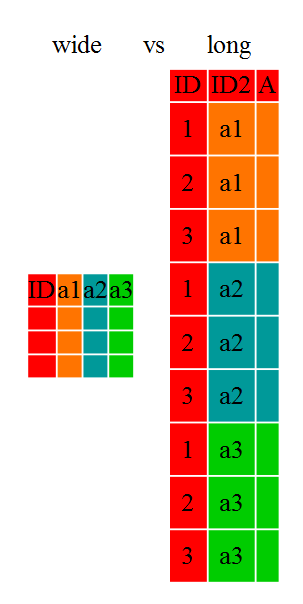
\includegraphics[width=0.7\linewidth]{img/tidyr-fig1} \end{center}

You may find data input may be simpler or some other applications may
prefer the ``wide'' format. However, many of R's functions have been
designed assuming you have ``long'' format data.

\section{Tidying the Gapminder Data}\label{tidying-the-gapminder-data}

Let's look at the structure of our original gapminder dataframe:

\begin{Shaded}
\begin{Highlighting}[]
\NormalTok{gap <-}\StringTok{ }\KeywordTok{read.csv}\NormalTok{(}\StringTok{"data/gapminder-FiveYearData.csv"}\NormalTok{, }\DataTypeTok{stringsAsFactors =} \OtherTok{TRUE}\NormalTok{)}
\KeywordTok{kable}\NormalTok{(}\KeywordTok{head}\NormalTok{(gap))}
\end{Highlighting}
\end{Shaded}

country

year

pop

continent

lifeExp

gdpPercap

Afghanistan

1952

8425333

Asia

28.8

779

Afghanistan

1957

9240934

Asia

30.3

821

Afghanistan

1962

10267083

Asia

32.0

853

Afghanistan

1967

11537966

Asia

34.0

836

Afghanistan

1972

13079460

Asia

36.1

740

Afghanistan

1977

14880372

Asia

38.4

786

\textbf{Question}: Is this data frame \textbf{wide} or \textbf{long}?

\textbf{Answer}: This data frame is somewhere in between the purely
`long' and `wide' formats. We have 3 ``ID variables''
(\texttt{continent}, \texttt{country}, \texttt{year}) and 3
``Observation variables'' (\texttt{pop}, \texttt{lifeExp},
\texttt{gdpPercap}).

Despite not having ALL observations in 1 column, this intermediate
format makes sense given that all 3 observation variables have different
units. As we have seen, many of the functions in R are often vector
based, and you usually do not want to do mathematical operations on
values with different units.

On the other hand, there are some instances in which a purely long or
wide format is ideal (e.g.~plotting). Likewise, sometimes you'll get
data on your desk that is poorly organized, and you'll need to
\textbf{reshape} it.

\section{\texorpdfstring{\texttt{tidyr}
functions}{tidyr functions}}\label{tidyr-functions}

Thankfully, the \texttt{tidyr} package will help you efficiently
transform your data regardless of original format.

\begin{Shaded}
\begin{Highlighting}[]
\CommentTok{# Install the "tidyr" package (only necessary one time)}
\CommentTok{# install.packages("tidyr") # Not Run}

\CommentTok{# Load the "tidyr" package (necessary every new R session)}
\KeywordTok{library}\NormalTok{(tidyr)}
\end{Highlighting}
\end{Shaded}

\subsection{\texorpdfstring{\texttt{gather}}{gather}}\label{gather}

Until now, we've been using the nicely formatted original gapminder
dataset. This dataset is not quite wide and not quite long -- it's
something in the middle, but `real' data (i.e.~our own research data)
will never be so well organized. Here let's start with the wide format
version of the gapminder dataset.

\begin{Shaded}
\begin{Highlighting}[]
\NormalTok{gap_wide <-}\StringTok{ }\KeywordTok{read.csv}\NormalTok{(}\StringTok{"data/gapminder_wide.csv"}\NormalTok{, }\DataTypeTok{stringsAsFactors =} \OtherTok{FALSE}\NormalTok{)}
\KeywordTok{kable}\NormalTok{(}\KeywordTok{head}\NormalTok{(gap_wide))}
\end{Highlighting}
\end{Shaded}

continent

country

gdpPercap\_1952

gdpPercap\_1957

gdpPercap\_1962

gdpPercap\_1967

gdpPercap\_1972

gdpPercap\_1977

gdpPercap\_1982

gdpPercap\_1987

gdpPercap\_1992

gdpPercap\_1997

gdpPercap\_2002

gdpPercap\_2007

lifeExp\_1952

lifeExp\_1957

lifeExp\_1962

lifeExp\_1967

lifeExp\_1972

lifeExp\_1977

lifeExp\_1982

lifeExp\_1987

lifeExp\_1992

lifeExp\_1997

lifeExp\_2002

lifeExp\_2007

pop\_1952

pop\_1957

pop\_1962

pop\_1967

pop\_1972

pop\_1977

pop\_1982

pop\_1987

pop\_1992

pop\_1997

pop\_2002

pop\_2007

Africa

Algeria

2449

3014

2551

3247

4183

4910

5745

5681

5023

4797

5288

6223

43.1

45.7

48.3

51.4

54.5

58.0

61.4

65.8

67.7

69.2

71.0

72.3

9279525

10270856

11000948

12760499

14760787

17152804

20033753

23254956

26298373

29072015

31287142

33333216

Africa

Angola

3521

3828

4269

5523

5473

3009

2757

2430

2628

2277

2773

4797

30.0

32.0

34.0

36.0

37.9

39.5

39.9

39.9

40.6

41.0

41.0

42.7

4232095

4561361

4826015

5247469

5894858

6162675

7016384

7874230

8735988

9875024

10866106

12420476

Africa

Benin

1063

960

949

1036

1086

1029

1278

1226

1191

1233

1373

1441

38.2

40.4

42.6

44.9

47.0

49.2

50.9

52.3

53.9

54.8

54.4

56.7

1738315

1925173

2151895

2427334

2761407

3168267

3641603

4243788

4981671

6066080

7026113

8078314

Africa

Botswana

851

918

984

1215

2264

3215

4551

6206

7954

8647

11004

12570

47.6

49.6

51.5

53.3

56.0

59.3

61.5

63.6

62.7

52.6

46.6

50.7

442308

474639

512764

553541

619351

781472

970347

1151184

1342614

1536536

1630347

1639131

Africa

Burkina Faso

543

617

723

795

855

743

807

912

932

946

1038

1217

32.0

34.9

37.8

40.7

43.6

46.1

48.1

49.6

50.3

50.3

50.6

52.3

4469979

4713416

4919632

5127935

5433886

5889574

6634596

7586551

8878303

10352843

12251209

14326203

Africa

Burundi

339

380

355

413

464

556

560

622

632

463

446

430

39.0

40.5

42.0

43.5

44.1

45.9

47.5

48.2

44.7

45.3

47.4

49.6

2445618

2667518

2961915

3330989

3529983

3834415

4580410

5126023

5809236

6121610

7021078

8390505

The first step towards getting our nice intermediate data format is to
first convert from the wide to the long format.

The function \texttt{gather()} will `gather' the observation variables
into a single variable. This is sometimes called ``melting'' your data,
because it melts the table from wide to long. Those data will be melted
into two variables: one for the variable names, and the other for the
variable values.

\begin{Shaded}
\begin{Highlighting}[]
\NormalTok{gap_long <-}\StringTok{ }\NormalTok{gap_wide }\OperatorTok
\StringTok{    }\KeywordTok{gather}\NormalTok{(obstype_year, obs_values, }\DecValTok{3}\OperatorTok{:}\DecValTok{38}\NormalTok{)}
\KeywordTok{kable}\NormalTok{(}\KeywordTok{head}\NormalTok{(gap_long))}
\end{Highlighting}
\end{Shaded}

continent

country

obstype\_year

obs\_values

Africa

Algeria

gdpPercap\_1952

2449

Africa

Angola

gdpPercap\_1952

3521

Africa

Benin

gdpPercap\_1952

1063

Africa

Botswana

gdpPercap\_1952

851

Africa

Burkina Faso

gdpPercap\_1952

543

Africa

Burundi

gdpPercap\_1952

339

Notice that we put 3 arguments into the \texttt{gather()} function:

\begin{enumerate}
\def\labelenumi{\arabic{enumi}.}
\tightlist
\item
  the name the new column for the new ID variable
  (\texttt{obstype\_year}),
\item
  the name for the new amalgamated observation variable
  (\texttt{obs\_value}),
\item
  the indices of the old observation variables (\texttt{3:38},
  signalling columns 3 through 38) that we want to gather into one
  variable. Notice that we don't want to melt down columns 1 and 2, as
  these are considered ``ID'' variables.
\end{enumerate}

We can also select observation variables using:

\begin{itemize}
\tightlist
\item
  variable indices
\item
  variable names (without quotes)
\item
  \texttt{x:z} to select all variables between x and z
\item
  \texttt{-y} to \emph{exclude} y
\item
  \texttt{starts\_with(x,\ ignore.case\ =\ TRUE)}: all names that starts
  with \texttt{x}
\item
  \texttt{ends\_with(x,\ ignore.case\ =\ TRUE)}: all names that ends
  with \texttt{x}
\item
  \texttt{contains(x,\ ignore.case\ =\ TRUE)}: all names that contain
  \texttt{x}
\end{itemize}

See the \texttt{select()} function in \texttt{dplyr} for more options.

For instance, here we do the same thing with (1) the
\texttt{starts\_with} function, and (2) the \texttt{-} operator:

\begin{Shaded}
\begin{Highlighting}[]
\CommentTok{# 1. with the starts_with() function}
\NormalTok{gap_long <-}\StringTok{ }\NormalTok{gap_wide }\OperatorTok
\StringTok{    }\KeywordTok{gather}\NormalTok{(obstype_year, obs_values, }\KeywordTok{starts_with}\NormalTok{(}\StringTok{'pop'}\NormalTok{),}
           \KeywordTok{starts_with}\NormalTok{(}\StringTok{'lifeExp'}\NormalTok{), }\KeywordTok{starts_with}\NormalTok{(}\StringTok{'gdpPercap'}\NormalTok{))}
\KeywordTok{kable}\NormalTok{(}\KeywordTok{head}\NormalTok{(gap_long))}
\end{Highlighting}
\end{Shaded}

continent

country

obstype\_year

obs\_values

Africa

Algeria

pop\_1952

9279525

Africa

Angola

pop\_1952

4232095

Africa

Benin

pop\_1952

1738315

Africa

Botswana

pop\_1952

442308

Africa

Burkina Faso

pop\_1952

4469979

Africa

Burundi

pop\_1952

2445618

\begin{Shaded}
\begin{Highlighting}[]

\CommentTok{# 2. with the - operator}
\NormalTok{gap_long <-}\StringTok{ }\NormalTok{gap_wide }\OperatorTok\StringTok{ }
\StringTok{  }\KeywordTok{gather}\NormalTok{(obstype_year, obs_values, }\OperatorTok{-}\NormalTok{continent, }\OperatorTok{-}\NormalTok{country)}
\KeywordTok{kable}\NormalTok{(}\KeywordTok{head}\NormalTok{(gap_long))}
\end{Highlighting}
\end{Shaded}

continent

country

obstype\_year

obs\_values

Africa

Algeria

gdpPercap\_1952

2449

Africa

Angola

gdpPercap\_1952

3521

Africa

Benin

gdpPercap\_1952

1063

Africa

Botswana

gdpPercap\_1952

851

Africa

Burkina Faso

gdpPercap\_1952

543

Africa

Burundi

gdpPercap\_1952

339

However you choose to do it, notice that the output collapses all of the
measure variables into two columns: one containing new ID variable, the
other containing the observation value for that row.

\subsection{\texorpdfstring{\texttt{separate}}{separate}}\label{separate}

You'll notice that in our long dataset, \texttt{obstype\_year} actually
contains 2 pieces of information, the observation type (\texttt{pop},
\texttt{lifeExp}, or \texttt{gdpPercap}) and the \texttt{year}.

We can use the \texttt{separate()} function to split the character
strings into multiple variables:

\begin{Shaded}
\begin{Highlighting}[]
\NormalTok{gap_long_sep <-}\StringTok{ }\NormalTok{gap_long }\OperatorTok\StringTok{ }
\StringTok{  }\KeywordTok{separate}\NormalTok{(obstype_year, }\DataTypeTok{into =} \KeywordTok{c}\NormalTok{(}\StringTok{'obs_type'}\NormalTok{,}\StringTok{'year'}\NormalTok{), }\DataTypeTok{sep =} \StringTok{"_"}\NormalTok{) }\OperatorTok\StringTok{ }
\StringTok{  }\KeywordTok{mutate}\NormalTok{(}\DataTypeTok{year =} \KeywordTok{as.integer}\NormalTok{(year))}
\KeywordTok{kable}\NormalTok{(}\KeywordTok{head}\NormalTok{(gap_long_sep))}
\end{Highlighting}
\end{Shaded}

continent

country

obs\_type

year

obs\_values

Africa

Algeria

gdpPercap

1952

2449

Africa

Angola

gdpPercap

1952

3521

Africa

Benin

gdpPercap

1952

1063

Africa

Botswana

gdpPercap

1952

851

Africa

Burkina Faso

gdpPercap

1952

543

Africa

Burundi

gdpPercap

1952

339

\subsection{\texorpdfstring{\texttt{spread}}{spread}}\label{spread}

The opposite of \texttt{gather()} is \texttt{spread()}. It spreads our
observation variables back out to make a wider table. We can use this
function to spread our \texttt{gap\_long()} to the original ``medium''
format.

\begin{Shaded}
\begin{Highlighting}[]
\NormalTok{gap_medium <-}\StringTok{ }\NormalTok{gap_long_sep }\OperatorTok\StringTok{ }
\StringTok{  }\KeywordTok{spread}\NormalTok{(obs_type, obs_values)}
\KeywordTok{kable}\NormalTok{(}\KeywordTok{head}\NormalTok{(gap_medium))}
\end{Highlighting}
\end{Shaded}

continent

country

year

gdpPercap

lifeExp

pop

Africa

Algeria

1952

2449

43.1

9279525

Africa

Algeria

1957

3014

45.7

10270856

Africa

Algeria

1962

2551

48.3

11000948

Africa

Algeria

1967

3247

51.4

12760499

Africa

Algeria

1972

4183

54.5

14760787

Africa

Algeria

1977

4910

58.0

17152804

All we need is some quick fixes to make this dataset identical to the
original \texttt{gapminder} dataset:

\begin{Shaded}
\begin{Highlighting}[]
\NormalTok{gap <-}\StringTok{ }\KeywordTok{read.csv}\NormalTok{(}\StringTok{"data/gapminder-FiveYearData.csv"}\NormalTok{)}
\KeywordTok{kable}\NormalTok{(}\KeywordTok{head}\NormalTok{(gap))}
\end{Highlighting}
\end{Shaded}

country

year

pop

continent

lifeExp

gdpPercap

Afghanistan

1952

8425333

Asia

28.8

779

Afghanistan

1957

9240934

Asia

30.3

821

Afghanistan

1962

10267083

Asia

32.0

853

Afghanistan

1967

11537966

Asia

34.0

836

Afghanistan

1972

13079460

Asia

36.1

740

Afghanistan

1977

14880372

Asia

38.4

786

\begin{Shaded}
\begin{Highlighting}[]
\CommentTok{# rearrange columns}
\NormalTok{gap_medium <-}\StringTok{ }\NormalTok{gap_medium[,}\KeywordTok{names}\NormalTok{(gap)]}
\KeywordTok{kable}\NormalTok{(}\KeywordTok{head}\NormalTok{(gap_medium))}
\end{Highlighting}
\end{Shaded}

country

year

pop

continent

lifeExp

gdpPercap

Algeria

1952

9279525

Africa

43.1

2449

Algeria

1957

10270856

Africa

45.7

3014

Algeria

1962

11000948

Africa

48.3

2551

Algeria

1967

12760499

Africa

51.4

3247

Algeria

1972

14760787

Africa

54.5

4183

Algeria

1977

17152804

Africa

58.0

4910

\begin{Shaded}
\begin{Highlighting}[]
\CommentTok{# arrange by country, continent, and year}
\NormalTok{gap_medium <-}\StringTok{ }\NormalTok{gap_medium }\OperatorTok\StringTok{ }
\StringTok{  }\KeywordTok{arrange}\NormalTok{(country,continent,year)}
\KeywordTok{kable}\NormalTok{(}\KeywordTok{head}\NormalTok{(gap_medium))}
\end{Highlighting}
\end{Shaded}

country

year

pop

continent

lifeExp

gdpPercap

Afghanistan

1952

8425333

Asia

28.8

779

Afghanistan

1957

9240934

Asia

30.3

821

Afghanistan

1962

10267083

Asia

32.0

853

Afghanistan

1967

11537966

Asia

34.0

836

Afghanistan

1972

13079460

Asia

36.1

740

Afghanistan

1977

14880372

Asia

38.4

786

\textbf{What we just told you will become obsolete\ldots{}}

\texttt{gather} and \texttt{spread} are being replaced by
\texttt{pivot\_longer} and \texttt{pivot\_wider} in
\texttt{tidyr\ 1.0.0}, which use ideas from the \texttt{cdata} package
to make reshaping easier to think about. In a future bootcamp, we'll
migrate to those functions.

\section{\texorpdfstring{More
\texttt{tidyverse}}{More tidyverse}}\label{more-tidyverse}

\texttt{dplyr} and \texttt{tidyr} have many more functions to help you
wrangle and manipulate your data. See the
\href{https://www.rstudio.com/wp-content/uploads/2015/02/data-wrangling-cheatsheet.pdf}{Data
Wrangling Cheat Sheet} for more.

There are some other useful packages in the
\href{http://www.tidyverse.org}{tidyverse}:

\begin{itemize}
\tightlist
\item
  \texttt{ggplot2} for plotting (we'll cover this in the Visualization
  module.)
\item
  \texttt{readr} and \texttt{haven} for reading in data
\item
  \texttt{purrr} for working iterations.
\item
  \texttt{stringr}, \texttt{lubridate}, \texttt{forcats} for
  manipulating strings, dates, and factors, respectively
\item
  many many more! Take a peak at the
  \href{https://github.com/tidyverse}{tidyverse github page}\ldots{}
\end{itemize}

**Pro \url{Tip:**} To install and load the core tidyverse packages
(includes \texttt{tidyr}, \texttt{dplyr}, and \texttt{ggplot2}, among
others), try:

\begin{Shaded}
\begin{Highlighting}[]
\NormalTok{## NOT run}
\CommentTok{# install.packages("tidyverse")}
\KeywordTok{library}\NormalTok{(tidyverse)}
\end{Highlighting}
\end{Shaded}

\section{Challenges}\label{challenges-12}

\begin{enumerate}
\def\labelenumi{\arabic{enumi}.}
\item
  Subset the results from challenge \#3 (above) to select only the
  \texttt{country}, \texttt{year}, and \texttt{gdpPercap\_diff} columns.
  Use \texttt{tidyr} put it in wide format so that countries are rows
  and years are columns.
\item
  Now turn the dataframe above back into the long format with three
  columns: \texttt{country}, \texttt{year}, and
  \texttt{gdpPercap\_diff}.
\end{enumerate}

\subsubsection*{Acknowledgments}\label{acknowledgments-4}
\addcontentsline{toc}{subsubsection}{Acknowledgments}

Some of these materials in this module were adapted from:

\begin{itemize}
\tightlist
\item
  \href{http://swcarpentry.github.io/r-novice-gapminder/}{Software
  Carpentry}
\item
  \href{https://github.com/berkeley-scf/r-bootcamp-fall-2019}{R bootcamp
  at UC Berkeley}
\end{itemize}

\begin{Shaded}
\begin{Highlighting}[]
\KeywordTok{library}\NormalTok{(kableExtra)}
\end{Highlighting}
\end{Shaded}

\chapter{Relational Data}\label{relational-data-1}

It's rare that a data analysis involves only a single table of data.
Typically you have many tables of data, and you must combine them to
answer the questions that you're interested in. Collectively, multiple
tables of data are called \textbf{relational data} because it is the
relations, not just the individual datasets, that are important.

Note that when we say relational database here, we are referring to how
the data are structured, not to the use of any fancy software.

\section{Why Relational Data}\label{why-relational-data}

As social scientists, we're often working with data across different
levels of analysis. The main principle of relational data is that each
table is structured around the same observational unit.

Why is this important? Check out the following data.

\begin{Shaded}
\begin{Highlighting}[]
\NormalTok{messy <-}\StringTok{ }\KeywordTok{data.frame}\NormalTok{(}
  \DataTypeTok{county =} \KeywordTok{c}\NormalTok{(}\DecValTok{36037}\NormalTok{, }\DecValTok{36038}\NormalTok{, }\DecValTok{36039}\NormalTok{, }\DecValTok{36040}\NormalTok{, }\OtherTok{NA}\NormalTok{ , }\DecValTok{37001}\NormalTok{, }\DecValTok{37002}\NormalTok{, }\DecValTok{37003}\NormalTok{),}
  \DataTypeTok{state =} \KeywordTok{c}\NormalTok{(}\StringTok{'NY'}\NormalTok{, }\StringTok{'NY'}\NormalTok{, }\StringTok{'NY'}\NormalTok{, }\OtherTok{NA}\NormalTok{, }\OtherTok{NA}\NormalTok{, }\StringTok{'VA'}\NormalTok{, }\StringTok{'VA'}\NormalTok{, }\StringTok{'VA'}\NormalTok{),}
  \DataTypeTok{cnty_pop =} \KeywordTok{c}\NormalTok{(}\DecValTok{3817735}\NormalTok{, }\DecValTok{422999}\NormalTok{, }\DecValTok{324920}\NormalTok{, }\DecValTok{143432}\NormalTok{, }\OtherTok{NA}\NormalTok{, }\DecValTok{3228290}\NormalTok{, }\DecValTok{449499}\NormalTok{, }\DecValTok{383888}\NormalTok{),}
  \DataTypeTok{state_pop =} \KeywordTok{c}\NormalTok{(}\DecValTok{43320903}\NormalTok{, }\DecValTok{43320903}\NormalTok{, }\OtherTok{NA}\NormalTok{, }\DecValTok{43320903}\NormalTok{, }\DecValTok{43320903}\NormalTok{, }\DecValTok{7173000}\NormalTok{, }\DecValTok{7173000}\NormalTok{, }\DecValTok{7173000}\NormalTok{),}
  \DataTypeTok{region =} \KeywordTok{c}\NormalTok{(}\DecValTok{1}\NormalTok{, }\DecValTok{1}\NormalTok{, }\DecValTok{1}\NormalTok{, }\DecValTok{1}\NormalTok{, }\DecValTok{1}\NormalTok{, }\DecValTok{3}\NormalTok{, }\DecValTok{3}\NormalTok{, }\DecValTok{4}\NormalTok{)}
\NormalTok{)}

\KeywordTok{kable}\NormalTok{(messy)}
\end{Highlighting}
\end{Shaded}

county

state

cnty\_pop

state\_pop

region

36037

NY

3817735

43320903

1

36038

NY

422999

43320903

1

36039

NY

324920

NA

1

36040

NA

143432

43320903

1

NA

NA

NA

43320903

1

37001

VA

3228290

7173000

3

37002

VA

449499

7173000

3

37003

VA

383888

7173000

4

What a mess! How can the population of the state of New York be 43
million for one county but ``missing'' for another? If this is a dataset
of counties, what does it mean when the ``county'' field is missing? If
region is something like Census region, how can two counties in the same
state be in different regions? And why is it that all the counties whose
codes start with 36 are in New York except for one, where the state is
unknown?

If we follow the principles of relational data, each type of
observational unit should form a table.

\begin{itemize}
\tightlist
\item
  counties contains data on counties.
\item
  states contains data on states
\end{itemize}

So our data should look like:

\begin{Shaded}
\begin{Highlighting}[]
\NormalTok{counties <-}\StringTok{ }\KeywordTok{data.frame}\NormalTok{(}
  \DataTypeTok{county =} \KeywordTok{c}\NormalTok{(}\DecValTok{36037}\NormalTok{, }\DecValTok{36038}\NormalTok{, }\DecValTok{36039}\NormalTok{, }\DecValTok{36040}\NormalTok{, }\DecValTok{37001}\NormalTok{, }\DecValTok{37002}\NormalTok{, }\DecValTok{37003}\NormalTok{),}
  \DataTypeTok{state =} \KeywordTok{c}\NormalTok{(}\StringTok{'NY'}\NormalTok{, }\StringTok{'NY'}\NormalTok{, }\StringTok{'NY'}\NormalTok{, }\StringTok{'NY'}\NormalTok{, }\StringTok{'VA'}\NormalTok{, }\StringTok{'VA'}\NormalTok{, }\StringTok{'VA'}\NormalTok{),}
  \DataTypeTok{county_pop =} \KeywordTok{c}\NormalTok{(}\DecValTok{3817735}\NormalTok{, }\DecValTok{422999}\NormalTok{, }\DecValTok{324920}\NormalTok{, }\DecValTok{143432}\NormalTok{, }\DecValTok{3228290}\NormalTok{, }\DecValTok{449499}\NormalTok{, }\DecValTok{383888}\NormalTok{), }\DataTypeTok{stringsAsFactors =}\NormalTok{ F}
\NormalTok{)}
\KeywordTok{kable}\NormalTok{(counties)}
\end{Highlighting}
\end{Shaded}

county

state

county\_pop

36037

NY

3817735

36038

NY

422999

36039

NY

324920

36040

NY

143432

37001

VA

3228290

37002

VA

449499

37003

VA

383888

\begin{Shaded}
\begin{Highlighting}[]

\NormalTok{states <-}\StringTok{ }\KeywordTok{data.frame}\NormalTok{(}
  \DataTypeTok{state =} \KeywordTok{c}\NormalTok{(}\StringTok{"NY"}\NormalTok{, }\StringTok{"VA"}\NormalTok{),}
  \DataTypeTok{state_pop =} \KeywordTok{c}\NormalTok{(}\DecValTok{43320903}\NormalTok{, }\DecValTok{7173000}\NormalTok{),}
  \DataTypeTok{region =} \KeywordTok{c}\NormalTok{(}\DecValTok{1}\NormalTok{, }\DecValTok{3}\NormalTok{), }\DataTypeTok{stringsAsFactors =}\NormalTok{ F}
\NormalTok{)}
\KeywordTok{kable}\NormalTok{(states)}
\end{Highlighting}
\end{Shaded}

state

state\_pop

region

NY

43320903

1

VA

7173000

3

County population is a property of a county, so it lives in the county
table. State population is a property of a state, so it cannot live in
the county table. If we had panel data on counties, we would need
separate tables for things that vary at the county level (like state)
and things that vary at the county-year level (like population).

Now the ambiguity is gone. Every county has a population and a state.
Every state has a population and a region. There are no missing states,
no missing counties, and no conflicting definitions. The database is
self-documenting.

\section{Keys}\label{keys-1}

The variables used to connect each pair of tables are called
\textbf{keys}. A key is a variable (or set of variables) that uniquely
identifies an observation. Also called a \emph{unique identifier}.

\begin{itemize}
\tightlist
\item
  Keys are complete. They never take on missing values.
\item
  Keys are unique. They are neer duplicated across rows of a table.
\end{itemize}

In simple cases, a single variable is sufficient to identify an
observation. In the example above, each county is identified with
\textbf{county} (a numeric identifier); each state is identified with
\textbf{state} (a two-letter string).

There are two types of keys:

\begin{itemize}
\item
  A \textbf{primary key} uniquely identifies an observation in its own
  table. For example, \texttt{counties\$county} is a primary key because
  it uniquely identifies each county in the counties table.
\item
  A \textbf{foreign key} uniquely identifies an observation in another
  table. For example, the counties\$state is a foreign key because it
  appears in the counties table where it matches each county to a unique
  state.
\end{itemize}

Sometimes a table doesn't have an explicit primary key: each row is an
observation, but no combination of variables reliably identifies it. If
a table lacks a primary key, it's useful to add one with
\texttt{mutate()} and \texttt{row\_number()}. This is called a
\textbf{surrogate key}.

A primary key and the corresponding foreign key in another table form a
\textbf{relation}.

\section{Joins}\label{joins}

Data stored in the form we have outlined above is considered
\emph{normalized}. In general, we should try to keep data normalized as
far into the code pipeline as we can. Storing normalized data means your
data will be easier to understand and it will be harder to make costly
mistakes.

At some point, however, we're going to have to merge (or \textbf{join})
the table together to produce a single dataframe, and conduct analysis
on that dataframe.

Let's say we wanted to merge tables \texttt{x} and \texttt{y}. A
\textbf{join} allows you to combine variables from the two tables. It
first matches observations by their keys, then copies across variables
from one table to the other.

There are four options:

\begin{enumerate}
\def\labelenumi{\arabic{enumi}.}
\tightlist
\item
  An \textbf{inner join} keeps observations that appear in both tables.
\item
  A \textbf{left join} keeps all observations in \texttt{x}.
\item
  A \textbf{right join} keeps all observations in \texttt{y}.
\item
  A \textbf{full join} keeps all observations in \texttt{x} and
  \texttt{y}.
\end{enumerate}

The most commonly used join is the \texttt{left\_join()}: you use this
whenever you look up additional data from another table, because it
preserves the original observations even when there isn't a match. For
example, a \texttt{left\_join()} on \texttt{x} and \texttt{y} pulls in
variables form \texttt{y} while preserving all the observations on
\texttt{x}.

Let's say we want to combine the \texttt{countries} and \texttt{states}
tables we created earlier.

\begin{Shaded}
\begin{Highlighting}[]
\NormalTok{counties_states <-}\StringTok{ }\NormalTok{counties }\OperatorTok
\StringTok{  }\KeywordTok{left_join}\NormalTok{(states, }\DataTypeTok{by =} \StringTok{"state"}\NormalTok{)}

\KeywordTok{kable}\NormalTok{(counties_states)}
\end{Highlighting}
\end{Shaded}

county

state

county\_pop

state\_pop

region

36037

NY

3817735

43320903

1

36038

NY

422999

43320903

1

36039

NY

324920

43320903

1

36040

NY

143432

43320903

1

37001

VA

3228290

7173000

3

37002

VA

449499

7173000

3

37003

VA

383888

7173000

3

Notice there are two new columns: \texttt{state\_pop} and
\texttt{region}.

The left join should be your default join: use it unless you have a
strong reason to prefer one of the others.

\section{Defining keys}\label{defining-keys}

In the example above, the two tables were joined by a single variable,
and that variable has the same name in both tables. That constraint was
encoded by \texttt{by\ =\ "key"}.

You can use other values for \texttt{by} to connect the tables in other
ways:

\begin{enumerate}
\def\labelenumi{\arabic{enumi}.}
\tightlist
\item
  The default, \textbf{\texttt{by\ =\ NULL}}, uses all variables that
  appear in both tables, the so called natural join.
\end{enumerate}

For example, let's say we wanted to add a column to the
\texttt{gapminder} dataset that encodes the regime type of each
country-year observation. We'll get that data from the \texttt{polityVI}
dataset.

\begin{Shaded}
\begin{Highlighting}[]
\NormalTok{gapminder <-}\StringTok{ }\KeywordTok{read.csv}\NormalTok{(}\StringTok{"data/gapminder.csv"}\NormalTok{, }\DataTypeTok{stringsAsFactors =}\NormalTok{ F)}
\NormalTok{polity <-}\StringTok{ }\KeywordTok{read.csv}\NormalTok{(}\StringTok{"data/polity_sub.csv"}\NormalTok{, }\DataTypeTok{stringsAsFactors =}\NormalTok{ F)}
\KeywordTok{kable}\NormalTok{(}\KeywordTok{head}\NormalTok{(polity))}
\end{Highlighting}
\end{Shaded}

country

year

polity2

Afghanistan

1800

-6

Afghanistan

1801

-6

Afghanistan

1802

-6

Afghanistan

1803

-6

Afghanistan

1804

-6

Afghanistan

1805

-6

We're now ready to join the tables. The common keys between them are
\texttt{country} and \texttt{year}:

\begin{Shaded}
\begin{Highlighting}[]
\NormalTok{gap1 <-}\StringTok{ }\NormalTok{gapminder }\OperatorTok
\StringTok{  }\KeywordTok{left_join}\NormalTok{(polity)}
\CommentTok{#> Joining, by = c("country", "year")}

\KeywordTok{kable}\NormalTok{(}\KeywordTok{head}\NormalTok{(gap1))}
\end{Highlighting}
\end{Shaded}

country

year

pop

continent

lifeExp

gdpPercap

polity2

Afghanistan

1952

8425333

Asia

28.8

779

-10

Afghanistan

1957

9240934

Asia

30.3

821

-10

Afghanistan

1962

10267083

Asia

32.0

853

-10

Afghanistan

1967

11537966

Asia

34.0

836

-7

Afghanistan

1972

13079460

Asia

36.1

740

-7

Afghanistan

1977

14880372

Asia

38.4

786

-7

\begin{enumerate}
\def\labelenumi{\arabic{enumi}.}
\setcounter{enumi}{1}
\item
  A character vector, \textbf{\texttt{by\ =\ c("x",\ "y")}}. This is
  like a natural join, but uses only some of the common variables.
\item
  A named character vector: \textbf{\texttt{by\ =\ c("a"\ =\ "b")}}.
  This will match variable \texttt{a} in table \texttt{x} to variable
  \texttt{b} in table \texttt{y}. The variables from \texttt{x} will be
  used in the output.
\end{enumerate}

For example, let's add another variable to our \texttt{gapminder}
dataset -- physical integrity rights -- from the CIRI dataset.

\begin{Shaded}
\begin{Highlighting}[]
\NormalTok{ciri <-}\StringTok{ }\KeywordTok{read.csv}\NormalTok{(}\StringTok{"data/ciri_sub.csv"}\NormalTok{, }\DataTypeTok{stringsAsFactors =}\NormalTok{ F)}
\KeywordTok{kable}\NormalTok{(}\KeywordTok{head}\NormalTok{(ciri))}
\end{Highlighting}
\end{Shaded}

CTRY

YEAR

PHYSINT

Afghanistan

1981

0

Afghanistan

1982

0

Afghanistan

1983

0

Afghanistan

1984

0

Afghanistan

1985

0

Afghanistan

1986

0

Both datasets have country and year columns, but they are named
differently.

\begin{Shaded}
\begin{Highlighting}[]
\NormalTok{gap2 <-}\StringTok{ }\NormalTok{gap1 }\OperatorTok
\StringTok{  }\KeywordTok{left_join}\NormalTok{(ciri, }\DataTypeTok{by =} \KeywordTok{c}\NormalTok{(}\StringTok{"country"}\NormalTok{ =}\StringTok{ "CTRY"}\NormalTok{, }\StringTok{"year"}\NormalTok{ =}\StringTok{ "YEAR"}\NormalTok{))}

\KeywordTok{kable}\NormalTok{(}\KeywordTok{head}\NormalTok{(gap2))}
\end{Highlighting}
\end{Shaded}

country

year

pop

continent

lifeExp

gdpPercap

polity2

PHYSINT

Afghanistan

1952

8425333

Asia

28.8

779

-10

NA

Afghanistan

1957

9240934

Asia

30.3

821

-10

NA

Afghanistan

1962

10267083

Asia

32.0

853

-10

NA

Afghanistan

1967

11537966

Asia

34.0

836

-7

NA

Afghanistan

1972

13079460

Asia

36.1

740

-7

NA

Afghanistan

1977

14880372

Asia

38.4

786

-7

NA

Notice that \texttt{PHYSINT} is \texttt{NA} in the first 6 rows because
the \texttt{ciri} dataset does not contain observations for Afghanistan
in these years. But because we used \texttt{left\_join()}, all
observations in \texttt{gapminder} were preserved.

We can see some values for \texttt{PHYSINT} if we peak at the bottom of
the dataset:

\begin{Shaded}
\begin{Highlighting}[]
\KeywordTok{kable}\NormalTok{(}\KeywordTok{tail}\NormalTok{(gap2))}
\end{Highlighting}
\end{Shaded}

country

year

pop

continent

lifeExp

gdpPercap

polity2

PHYSINT

1699

Zimbabwe

1982

7636524

Africa

60.4

789

4

5

1700

Zimbabwe

1987

9216418

Africa

62.4

706

-6

5

1701

Zimbabwe

1992

10704340

Africa

60.4

693

-6

5

1702

Zimbabwe

1997

11404948

Africa

46.8

792

-6

6

1703

Zimbabwe

2002

11926563

Africa

40.0

672

-4

2

1704

Zimbabwe

2007

12311143

Africa

43.5

470

-4

1

\section{Duplicate keys}\label{duplicate-keys}

So far we have assumed that the keys are unique. But that's not always
the case. For example,

\begin{Shaded}
\begin{Highlighting}[]
\NormalTok{x <-}\StringTok{ }\KeywordTok{data.frame}\NormalTok{(}\DataTypeTok{key =} \KeywordTok{c}\NormalTok{(}\DecValTok{1}\NormalTok{, }\DecValTok{2}\NormalTok{),}
               \DataTypeTok{val_y =} \KeywordTok{c}\NormalTok{(}\StringTok{"x1"}\NormalTok{, }\StringTok{"x2"}\NormalTok{))}

\NormalTok{y <-}\StringTok{ }\KeywordTok{data.frame}\NormalTok{(}\DataTypeTok{key =} \KeywordTok{c}\NormalTok{(}\DecValTok{1}\NormalTok{, }\DecValTok{2}\NormalTok{, }\DecValTok{2}\NormalTok{, }\DecValTok{1}\NormalTok{),}
               \DataTypeTok{val_x =} \KeywordTok{c}\NormalTok{(}\StringTok{"y1"}\NormalTok{, }\StringTok{"y2"}\NormalTok{, }\StringTok{"y3"}\NormalTok{, }\StringTok{"y4"}\NormalTok{))}

\KeywordTok{left_join}\NormalTok{(x, y, }\DataTypeTok{by =} \StringTok{"key"}\NormalTok{)}
\CommentTok{#>   key val_y val_x}
\CommentTok{#> 1   1    x1    y1}
\CommentTok{#> 2   1    x1    y4}
\CommentTok{#> 3   2    x2    y2}
\CommentTok{#> 4   2    x2    y3}
\end{Highlighting}
\end{Shaded}

Notice that this can sometimes cause unintended duplicates.

\subsubsection*{Acknowledgements}\label{acknowledgements-2}
\addcontentsline{toc}{subsubsection}{Acknowledgements}

This page is in part derived from the following sources:

\begin{enumerate}
\def\labelenumi{\arabic{enumi}.}
\item
  \href{https://r4ds.had.co.nz}{R for Data Science} licensed under
  \href{https://creativecommons.org/licenses/by-nc-nd/3.0/us/}{Creative
  Commons Attribution-NonCommercial-NoDerivs 3.0}
\item
  \href{https://web.stanford.edu/~gentzkow/research/CodeAndData.pdf}{Gentzkow,
  Matthew and Jesse M. Shapiro. 2014. Code and Data for the Social
  Sciences: A Practitioner's Guide.}
\end{enumerate}

\begin{quote}
``Make it informative, then make it pretty''
\end{quote}

\chapter{Plotting}\label{plotting}

There are two major sets of tools for creating plots in R:

\begin{itemize}
\item
  \begin{enumerate}
  \def\labelenumi{\arabic{enumi}.}
  \tightlist
  \item
    \protect\hyperlink{1-r-base-graphics}{base}, which come with all R
    installations
  \end{enumerate}
\item
  \begin{enumerate}
  \def\labelenumi{\arabic{enumi}.}
  \setcounter{enumi}{1}
  \tightlist
  \item
    \protect\hyperlink{2-ggplot2}{ggplot2}, a stand-alone package.
  \end{enumerate}
\end{itemize}

Note that other plotting facilities do exist (notably \textbf{lattice}),
but base and ggplot2 are by far the most popular.

\section{The dataset}\label{the-dataset}

For the following examples, we will using the gapminder dataset we were
playing around with earlier Gapminder is a country-year dataset with
information on life expectancy, among other things.

\begin{Shaded}
\begin{Highlighting}[]
\NormalTok{gap <-}\StringTok{ }\KeywordTok{read.csv}\NormalTok{(}\StringTok{"data/gapminder-FiveYearData.csv"}\NormalTok{, }\DataTypeTok{stringsAsFactors =}\NormalTok{ F)}
\end{Highlighting}
\end{Shaded}

\section{R base graphics}\label{r-base-graphics}

The \textbf{basic} call takes the following form:

\begin{Shaded}
\begin{Highlighting}[]
\KeywordTok{plot}\NormalTok{(}\DataTypeTok{x=}\NormalTok{, }\DataTypeTok{y=}\NormalTok{)}
\end{Highlighting}
\end{Shaded}

\begin{Shaded}
\begin{Highlighting}[]
\KeywordTok{plot}\NormalTok{(}\DataTypeTok{x =}\NormalTok{ gap}\OperatorTok{$}\NormalTok{gdpPercap, }\DataTypeTok{y =}\NormalTok{ gap}\OperatorTok{$}\NormalTok{lifeExp)}
\end{Highlighting}
\end{Shaded}

\begin{center}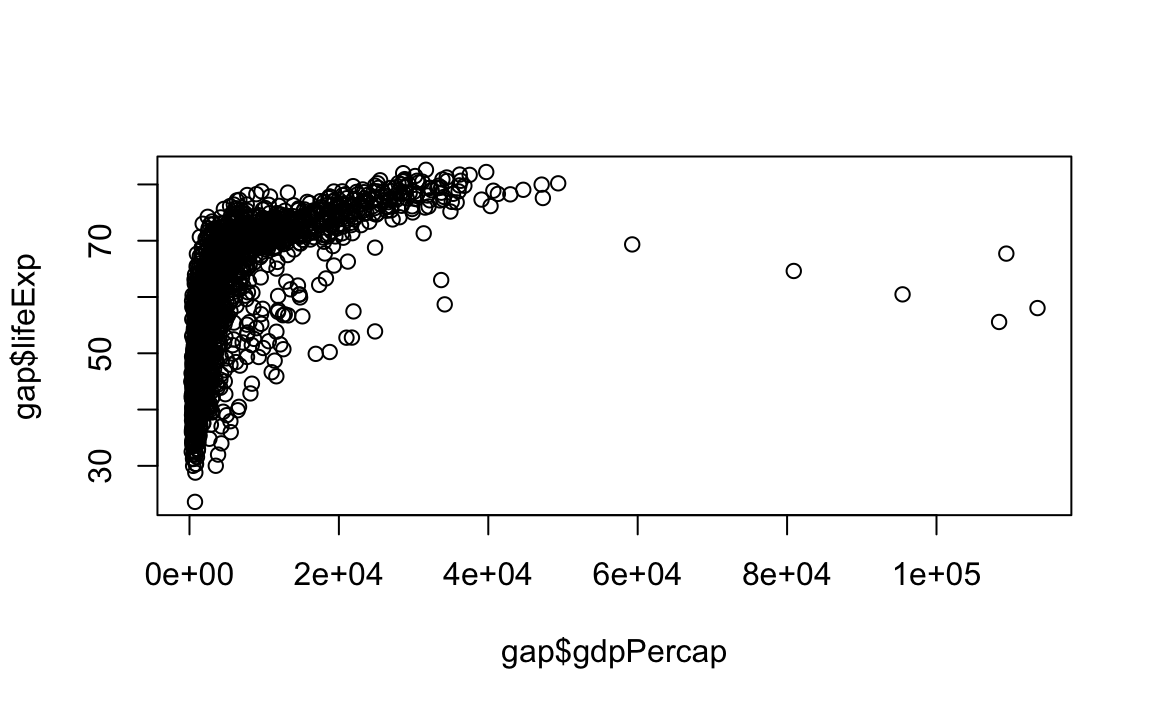
\includegraphics[width=0.7\linewidth]{site1_files/figure-latex/unnamed-chunk-264-1} \end{center}

\subsection{Scatter and Line Plots}\label{scatter-and-line-plots}

The ``type'' argument accepts the following character indicators.

\begin{itemize}
\tightlist
\item
  ``p'' -- point/scatter plots (default plotting behavior)
\end{itemize}

\begin{Shaded}
\begin{Highlighting}[]
\KeywordTok{plot}\NormalTok{(}\DataTypeTok{x =}\NormalTok{ gap}\OperatorTok{$}\NormalTok{gdpPercap, }\DataTypeTok{y =}\NormalTok{ gap}\OperatorTok{$}\NormalTok{lifeExp, }\DataTypeTok{type=}\StringTok{"p"}\NormalTok{)}
\end{Highlighting}
\end{Shaded}

\begin{figure}

{\centering 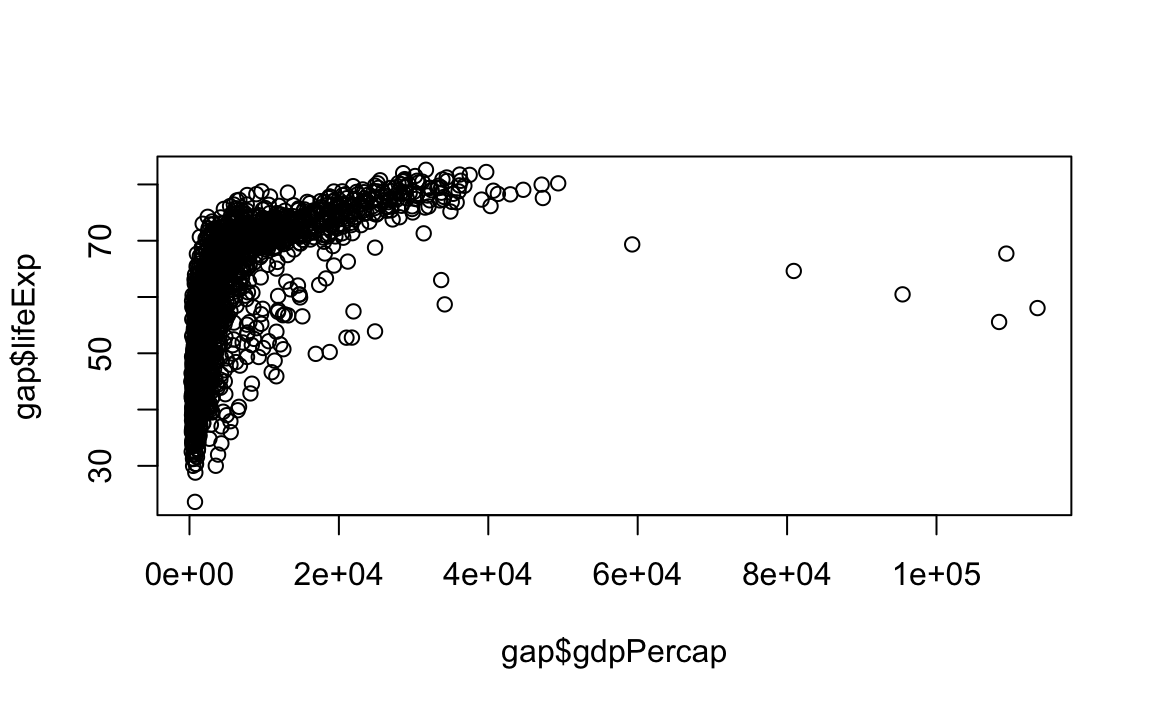
\includegraphics[width=0.7\linewidth]{site1_files/figure-latex/unnamed-chunk-265-1} 

}

\caption{ }\label{fig:unnamed-chunk-265}
\end{figure}

\begin{itemize}
\tightlist
\item
  ``l'' -- line graphs
\end{itemize}

\begin{Shaded}
\begin{Highlighting}[]
\CommentTok{# Note that "line" does not create a smoothing line, just connected points}
\KeywordTok{plot}\NormalTok{(}\DataTypeTok{x =}\NormalTok{ gap}\OperatorTok{$}\NormalTok{gdpPercap, }\DataTypeTok{y =}\NormalTok{ gap}\OperatorTok{$}\NormalTok{lifeExp, }\DataTypeTok{type=}\StringTok{"l"}\NormalTok{) }
\end{Highlighting}
\end{Shaded}

\begin{figure}

{\centering 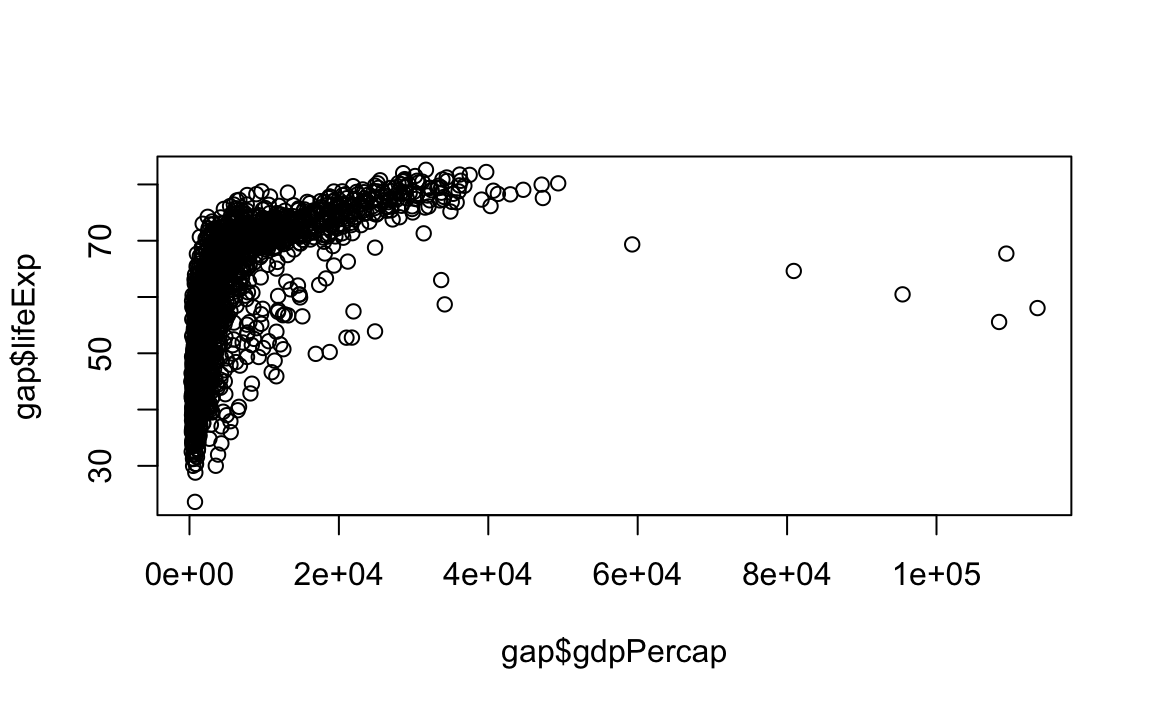
\includegraphics[width=0.7\linewidth]{site1_files/figure-latex/unnamed-chunk-266-1} 

}

\caption{ }\label{fig:unnamed-chunk-266}
\end{figure}

\begin{itemize}
\tightlist
\item
  ``b'' -- both line and point plots
\end{itemize}

\begin{Shaded}
\begin{Highlighting}[]
\KeywordTok{plot}\NormalTok{(}\DataTypeTok{x =}\NormalTok{ gap}\OperatorTok{$}\NormalTok{gdpPercap, }\DataTypeTok{y =}\NormalTok{ gap}\OperatorTok{$}\NormalTok{lifeExp, }\DataTypeTok{type=}\StringTok{"b"}\NormalTok{) }
\end{Highlighting}
\end{Shaded}

\begin{figure}

{\centering 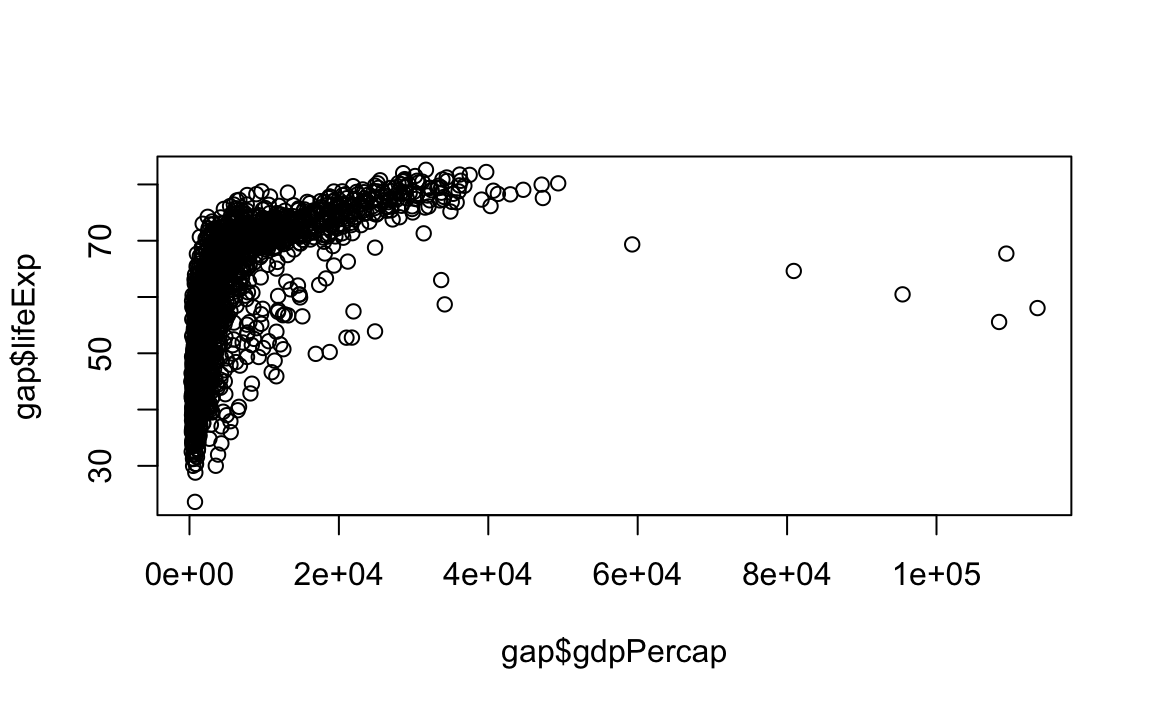
\includegraphics[width=0.7\linewidth]{site1_files/figure-latex/unnamed-chunk-267-1} 

}

\caption{ }\label{fig:unnamed-chunk-267}
\end{figure}

\subsection{Histograms and density
plots}\label{histograms-and-density-plots}

Histograms display the frequency of different values of a variable.

\begin{Shaded}
\begin{Highlighting}[]
\KeywordTok{hist}\NormalTok{(}\DataTypeTok{x=}\NormalTok{gap}\OperatorTok{$}\NormalTok{lifeExp)}
\end{Highlighting}
\end{Shaded}

\begin{center}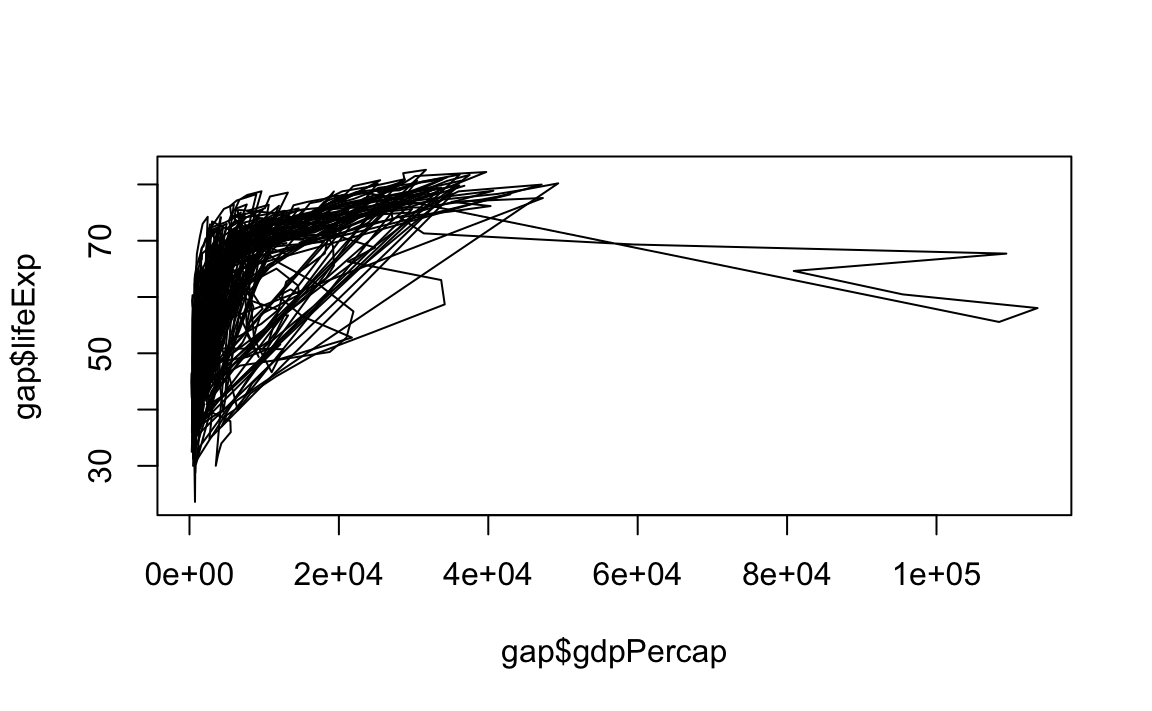
\includegraphics[width=0.7\linewidth]{site1_files/figure-latex/unnamed-chunk-268-1} \end{center}

Histograms require a \texttt{break} argument, which determine the number
of bins in the plot. Let's play around with different \texttt{break}
values.

\begin{Shaded}
\begin{Highlighting}[]
\KeywordTok{hist}\NormalTok{(}\DataTypeTok{x=}\NormalTok{gap}\OperatorTok{$}\NormalTok{lifeExp, }\DataTypeTok{breaks=}\DecValTok{5}\NormalTok{)}
\KeywordTok{hist}\NormalTok{(}\DataTypeTok{x=}\NormalTok{gap}\OperatorTok{$}\NormalTok{lifeExp, }\DataTypeTok{breaks=}\DecValTok{10}\NormalTok{)}
\end{Highlighting}
\end{Shaded}

\begin{center}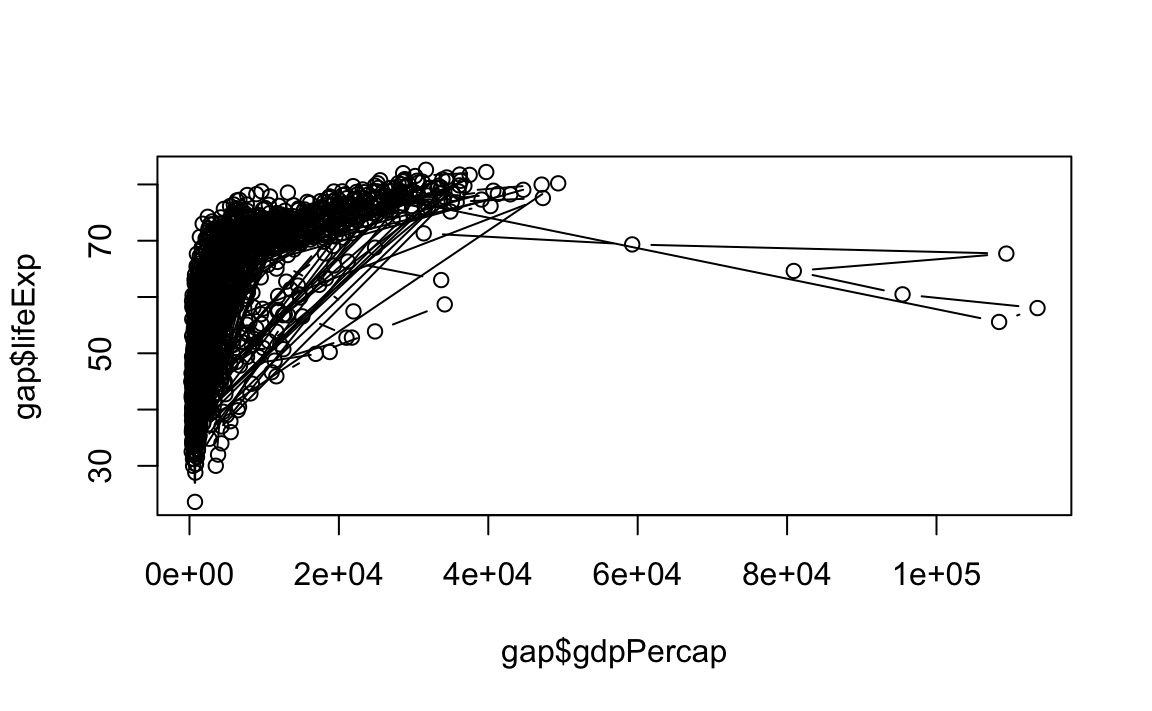
\includegraphics[width=0.7\linewidth]{site1_files/figure-latex/unnamed-chunk-269-1} 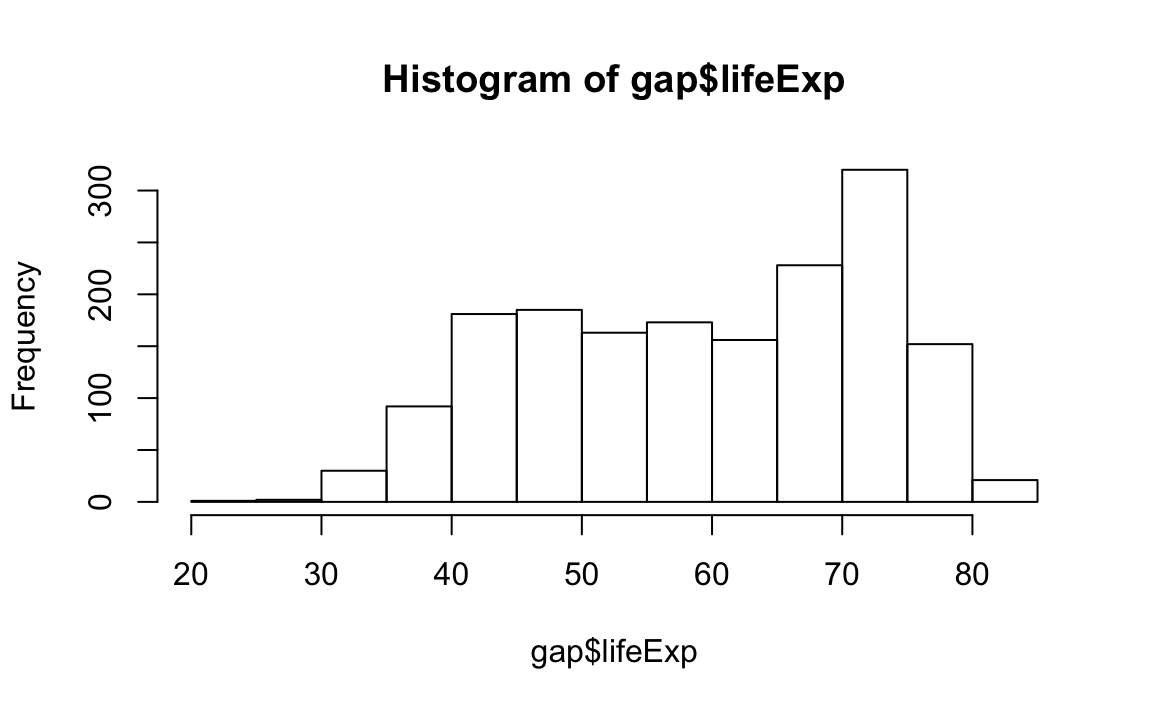
\includegraphics[width=0.7\linewidth]{site1_files/figure-latex/unnamed-chunk-269-2} \end{center}

Density plots are similar, they visualises the distribution of data over
a continuous interval.

\begin{Shaded}
\begin{Highlighting}[]
\CommentTok{# Create a density object (}\AlertTok{NOTE}\CommentTok{: be sure to remove missing values)}
\NormalTok{age.density <-}\StringTok{ }\KeywordTok{density}\NormalTok{(}\DataTypeTok{x=}\NormalTok{gap}\OperatorTok{$}\NormalTok{lifeExp, }\DataTypeTok{na.rm=}\NormalTok{T)}

\CommentTok{# Plot the density object}
\KeywordTok{plot}\NormalTok{(}\DataTypeTok{x=}\NormalTok{age.density)}
\end{Highlighting}
\end{Shaded}

\begin{figure}

{\centering 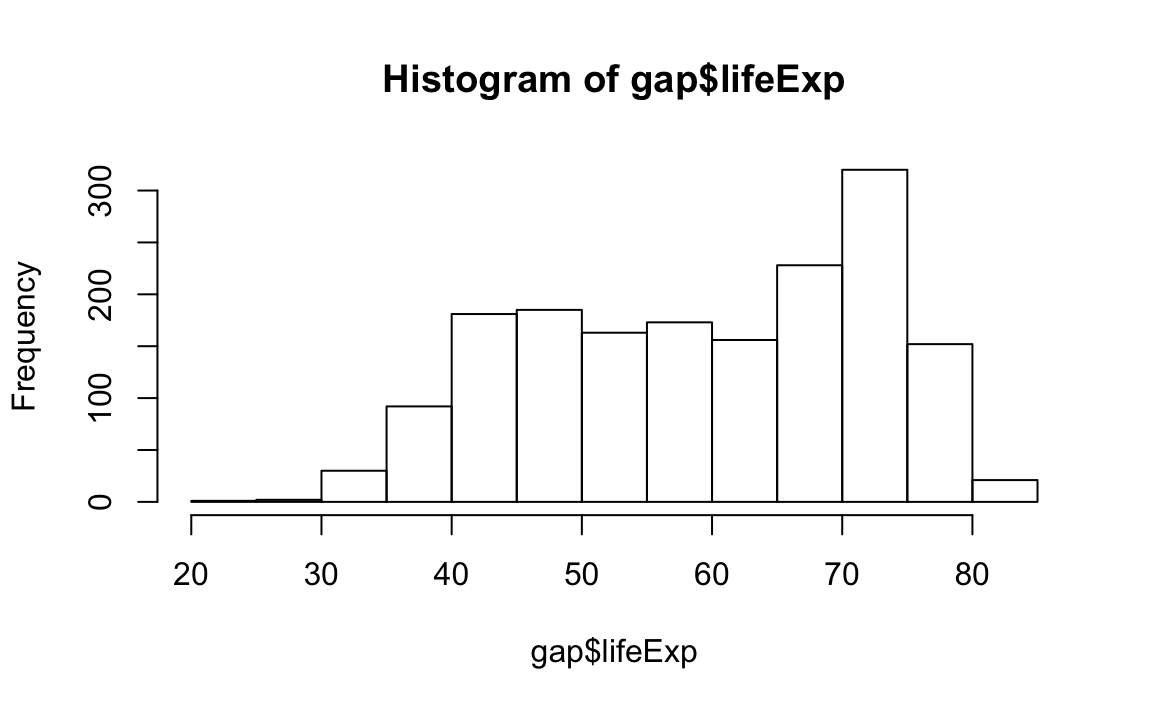
\includegraphics[width=0.7\linewidth]{site1_files/figure-latex/unnamed-chunk-270-1} 

}

\caption{ }\label{fig:unnamed-chunk-270}
\end{figure}

Density passes a \texttt{bw} parameter, which determins the plot's
``bandwidth''.

\begin{Shaded}
\begin{Highlighting}[]
\CommentTok{# Plot the density object, bandwidth of 0.5}
\KeywordTok{plot}\NormalTok{(}\DataTypeTok{x=}\KeywordTok{density}\NormalTok{(}\DataTypeTok{x=}\NormalTok{gap}\OperatorTok{$}\NormalTok{lifeExp, }\DataTypeTok{bw=}\NormalTok{.}\DecValTok{5}\NormalTok{))}
\CommentTok{# Plot the density object, bandwidth of 2}
\KeywordTok{plot}\NormalTok{(}\DataTypeTok{x=}\KeywordTok{density}\NormalTok{(}\DataTypeTok{x=}\NormalTok{gap}\OperatorTok{$}\NormalTok{lifeExp, }\DataTypeTok{bw=}\DecValTok{2}\NormalTok{))}
\CommentTok{# Plot the density object, bandwidth of 6}
\KeywordTok{plot}\NormalTok{(}\DataTypeTok{x=}\KeywordTok{density}\NormalTok{(}\DataTypeTok{x=}\NormalTok{gap}\OperatorTok{$}\NormalTok{lifeExp, }\DataTypeTok{bw=}\DecValTok{6}\NormalTok{)) }
\end{Highlighting}
\end{Shaded}

\begin{center}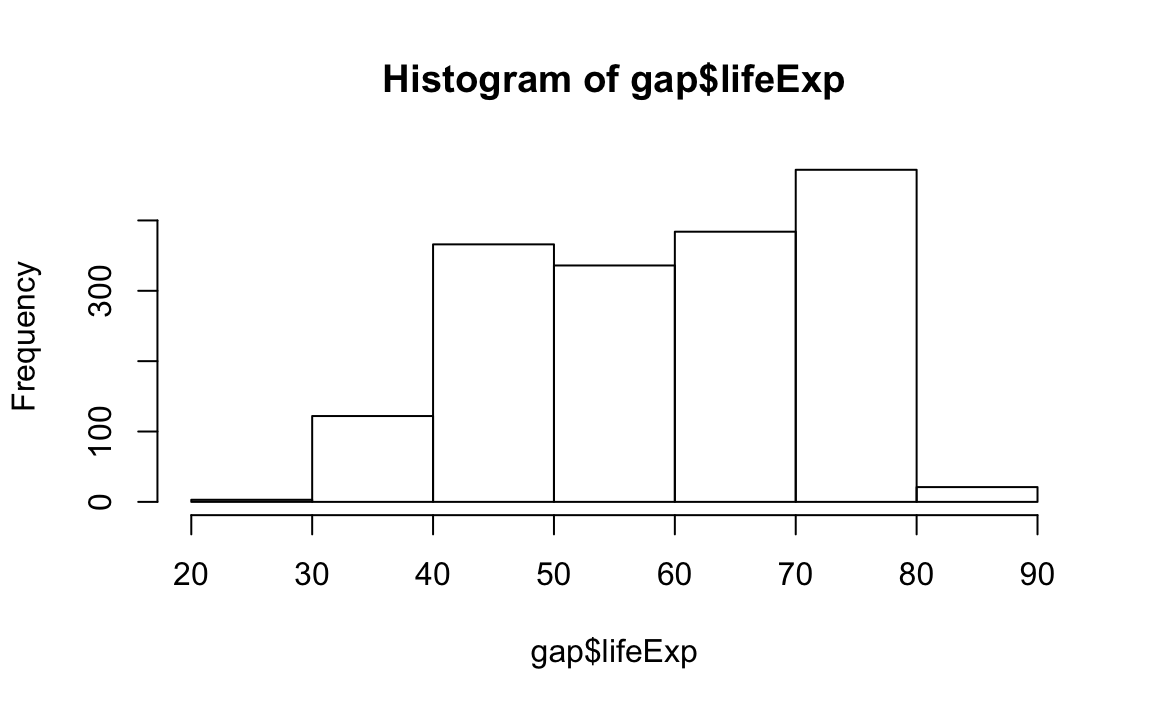
\includegraphics[width=0.7\linewidth]{site1_files/figure-latex/unnamed-chunk-271-1} 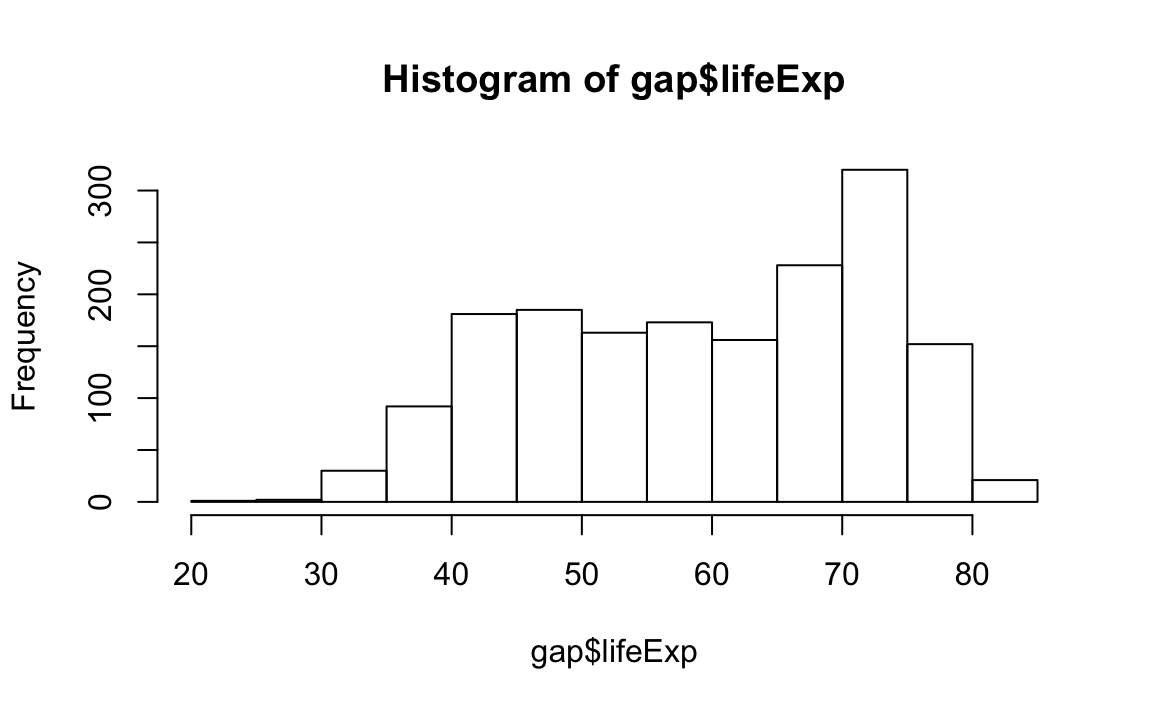
\includegraphics[width=0.7\linewidth]{site1_files/figure-latex/unnamed-chunk-271-2} 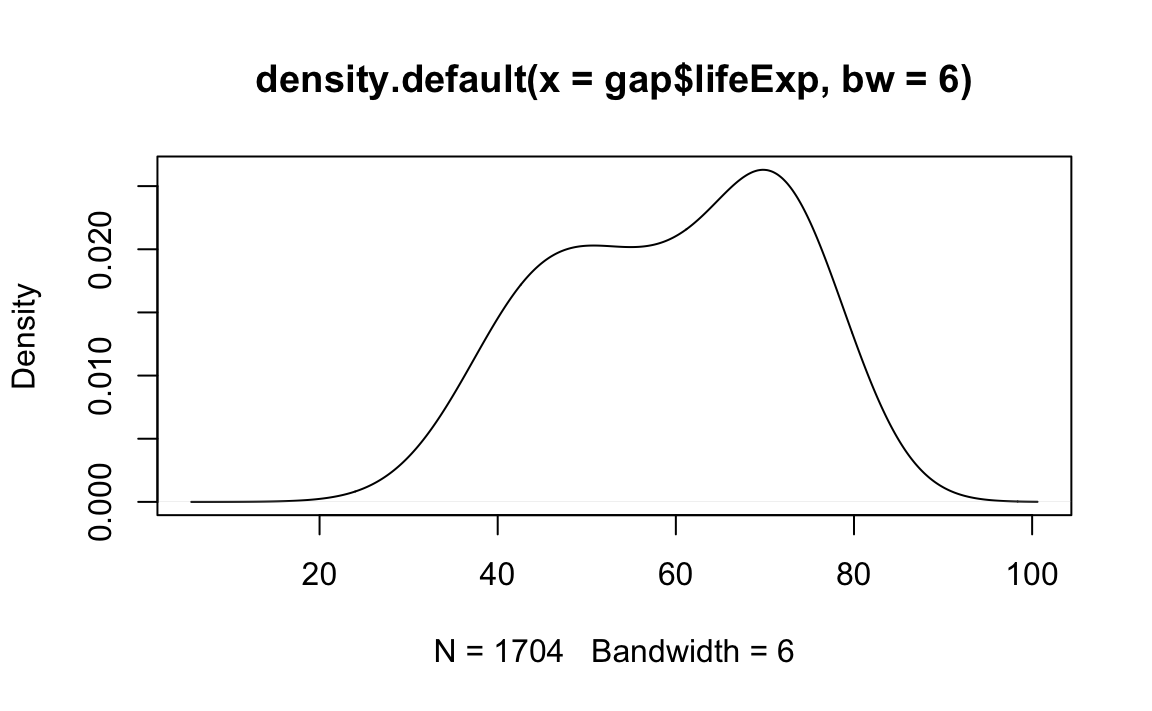
\includegraphics[width=0.7\linewidth]{site1_files/figure-latex/unnamed-chunk-271-3} \end{center}

\subsection{Labels}\label{labels}

Here's the basic call with popular labeling arguments:

\begin{Shaded}
\begin{Highlighting}[]
\KeywordTok{plot}\NormalTok{(}\DataTypeTok{x=}\NormalTok{, }\DataTypeTok{y=}\NormalTok{, }\DataTypeTok{type=}\StringTok{""}\NormalTok{, }\DataTypeTok{xlab=}\StringTok{""}\NormalTok{, }\DataTypeTok{ylab=}\StringTok{""}\NormalTok{, }\DataTypeTok{main=}\StringTok{""}\NormalTok{) }
\end{Highlighting}
\end{Shaded}

From the previous example\ldots{}

\begin{Shaded}
\begin{Highlighting}[]
\KeywordTok{plot}\NormalTok{(}\DataTypeTok{x =}\NormalTok{ gap}\OperatorTok{$}\NormalTok{gdpPercap, }\DataTypeTok{y =}\NormalTok{ gap}\OperatorTok{$}\NormalTok{lifeExp, }\DataTypeTok{type=}\StringTok{"p"}\NormalTok{, }\DataTypeTok{xlab=}\StringTok{"GDP per cap"}\NormalTok{, }\DataTypeTok{ylab=}\StringTok{"Life Expectancy"}\NormalTok{, }\DataTypeTok{main=}\StringTok{"Life Expectancy ~ GDP"}\NormalTok{) }\CommentTok{# Add labels for axes and overall plot}
\end{Highlighting}
\end{Shaded}

\begin{figure}

{\centering 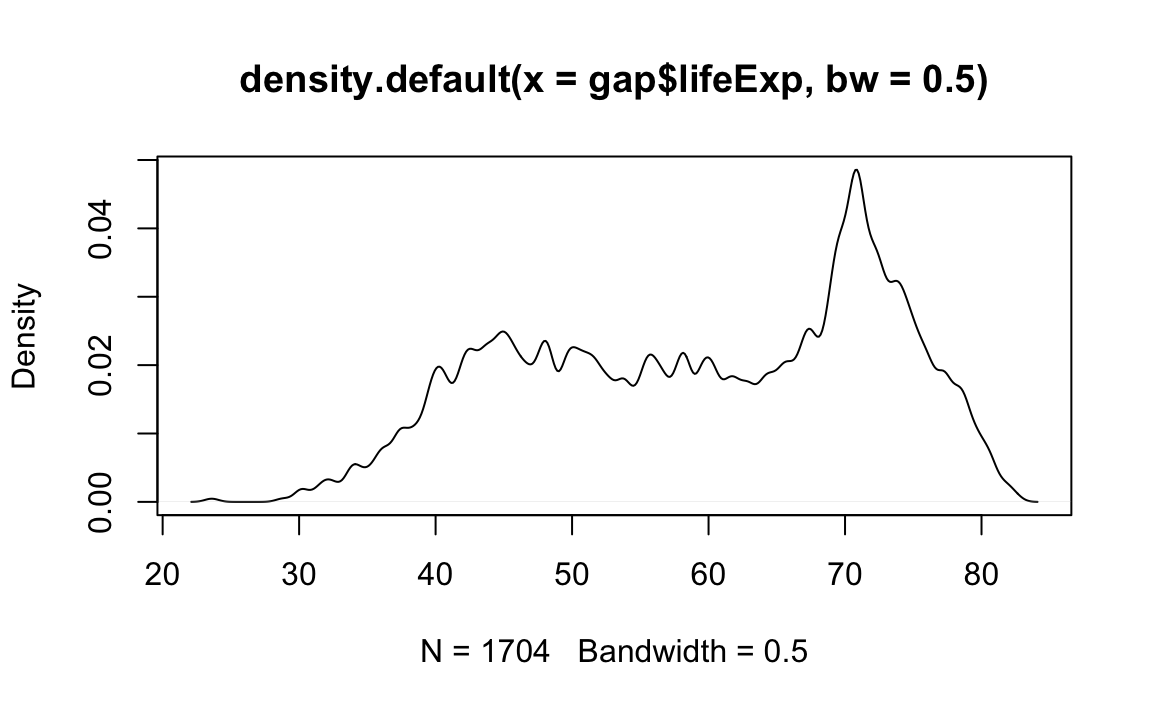
\includegraphics[width=0.7\linewidth]{site1_files/figure-latex/unnamed-chunk-273-1} 

}

\caption{ }\label{fig:unnamed-chunk-273}
\end{figure}

\subsection{Axis and size scaling}\label{axis-and-size-scaling}

Currently it's hard to see the relationship between the points due to
some strong outliers in GDP per capita. We can change the scale of units
on the x axis using scaling arguments.

Here's the Bbsic call with popular scaling arguments

\begin{Shaded}
\begin{Highlighting}[]
\KeywordTok{plot}\NormalTok{(}\DataTypeTok{x=}\NormalTok{, }\DataTypeTok{y=}\NormalTok{, }\DataTypeTok{type=}\StringTok{""}\NormalTok{, }\DataTypeTok{xlim=}\NormalTok{, }\DataTypeTok{ylim=}\NormalTok{, }\DataTypeTok{cex=}\NormalTok{)}
\end{Highlighting}
\end{Shaded}

From the previous example\ldots{}

\begin{Shaded}
\begin{Highlighting}[]
\CommentTok{# Create a basic plot}
\KeywordTok{plot}\NormalTok{(}\DataTypeTok{x =}\NormalTok{ gap}\OperatorTok{$}\NormalTok{gdpPercap, }\DataTypeTok{y =}\NormalTok{ gap}\OperatorTok{$}\NormalTok{lifeExp, }\DataTypeTok{type=}\StringTok{"p"}\NormalTok{)}
\CommentTok{# Limit gdp (x-axis) to between 1,000 and 20,000}
\KeywordTok{plot}\NormalTok{(}\DataTypeTok{x =}\NormalTok{ gap}\OperatorTok{$}\NormalTok{gdpPercap, }\DataTypeTok{y =}\NormalTok{ gap}\OperatorTok{$}\NormalTok{lifeExp, }\DataTypeTok{xlim =} \KeywordTok{c}\NormalTok{(}\DecValTok{1000}\NormalTok{,}\DecValTok{20000}\NormalTok{)) }
\CommentTok{# Limit gdp (x-axis) to between 1,000 and 20,000, increase point size to 2}
\KeywordTok{plot}\NormalTok{(}\DataTypeTok{x =}\NormalTok{ gap}\OperatorTok{$}\NormalTok{gdpPercap, }\DataTypeTok{y =}\NormalTok{ gap}\OperatorTok{$}\NormalTok{lifeExp, }\DataTypeTok{xlim =} \KeywordTok{c}\NormalTok{(}\DecValTok{1000}\NormalTok{,}\DecValTok{20000}\NormalTok{), }\DataTypeTok{cex=}\DecValTok{2}\NormalTok{) }
\CommentTok{# Limit gdp (x-axis) to between 1,000 and 20,000, decrease point size to 0.5}
\KeywordTok{plot}\NormalTok{(}\DataTypeTok{x =}\NormalTok{ gap}\OperatorTok{$}\NormalTok{gdpPercap, }\DataTypeTok{y =}\NormalTok{ gap}\OperatorTok{$}\NormalTok{lifeExp, }\DataTypeTok{xlim =} \KeywordTok{c}\NormalTok{(}\DecValTok{1000}\NormalTok{,}\DecValTok{20000}\NormalTok{), }\DataTypeTok{cex=}\FloatTok{0.5}\NormalTok{)  }
\end{Highlighting}
\end{Shaded}

\begin{figure}

{\centering 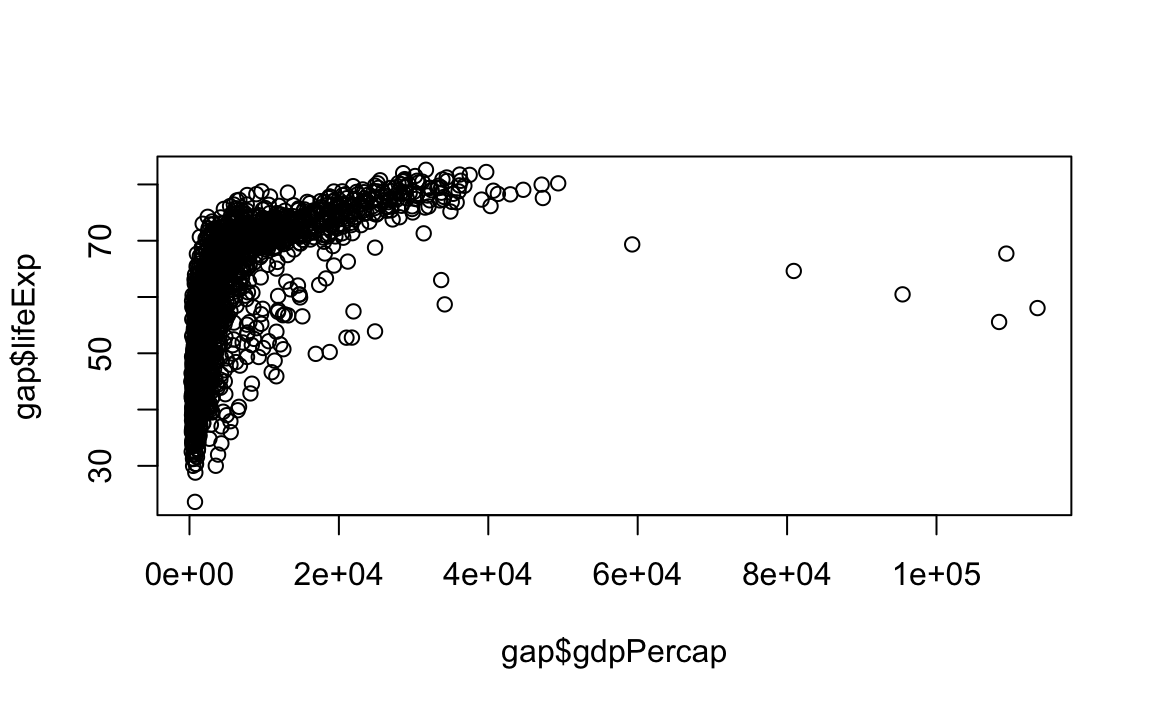
\includegraphics[width=0.7\linewidth]{site1_files/figure-latex/unnamed-chunk-275-1} 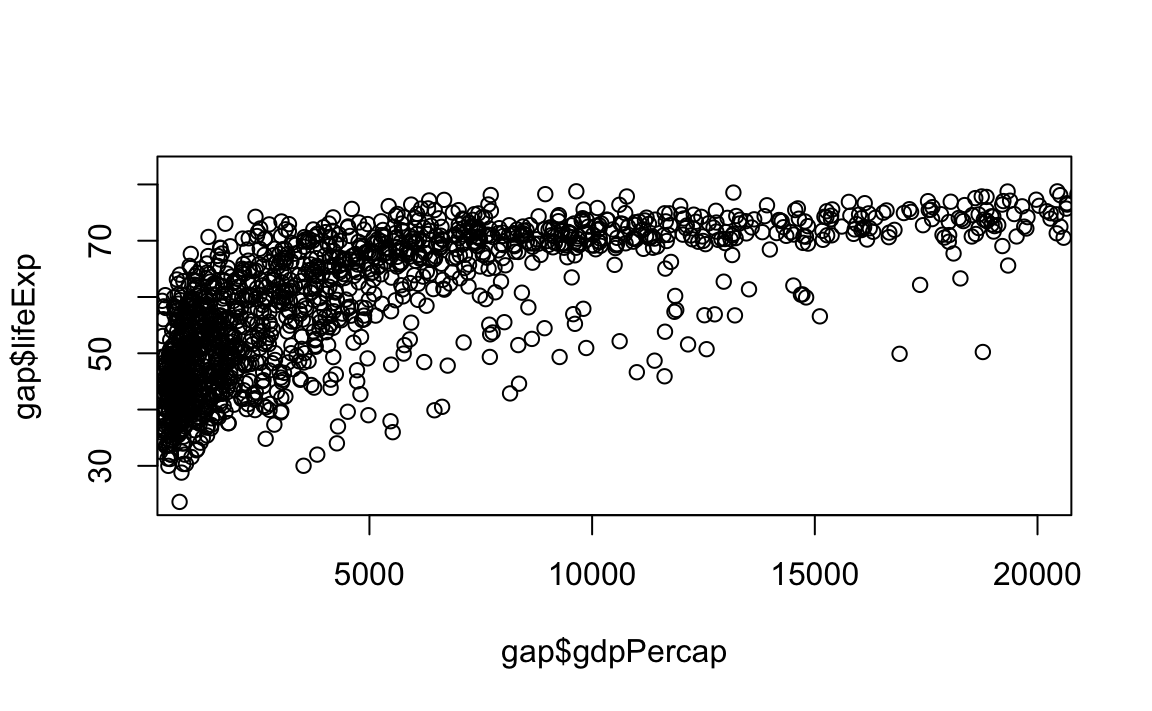
\includegraphics[width=0.7\linewidth]{site1_files/figure-latex/unnamed-chunk-275-2} 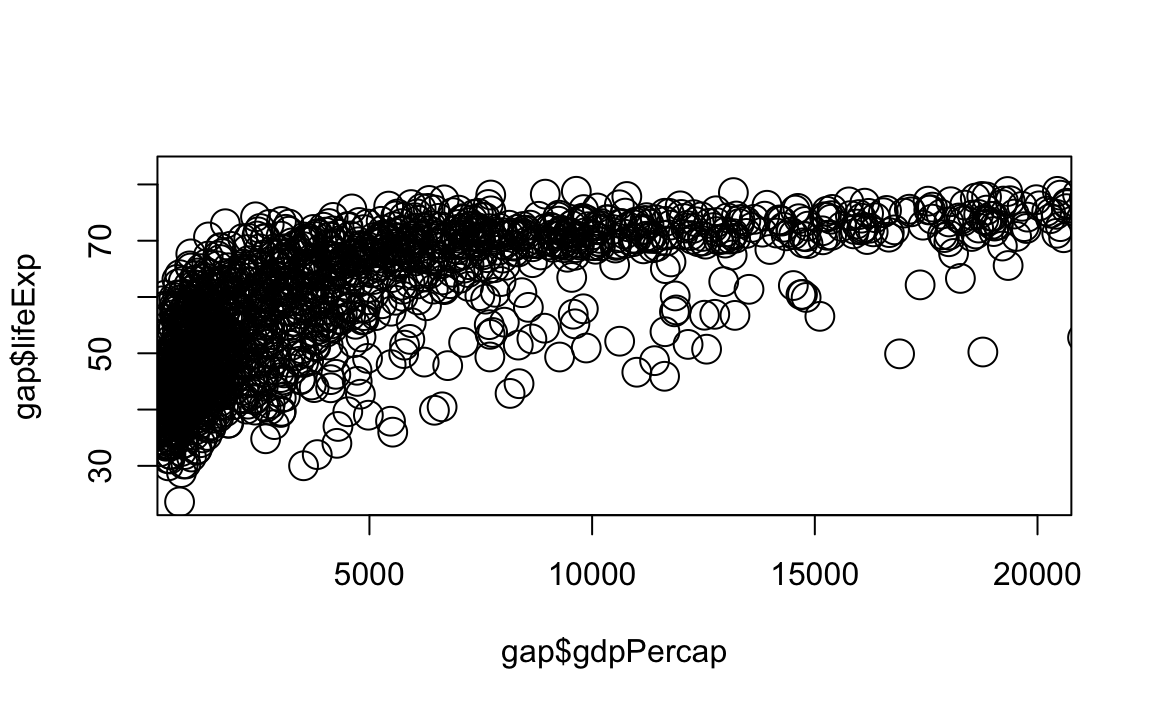
\includegraphics[width=0.7\linewidth]{site1_files/figure-latex/unnamed-chunk-275-3} 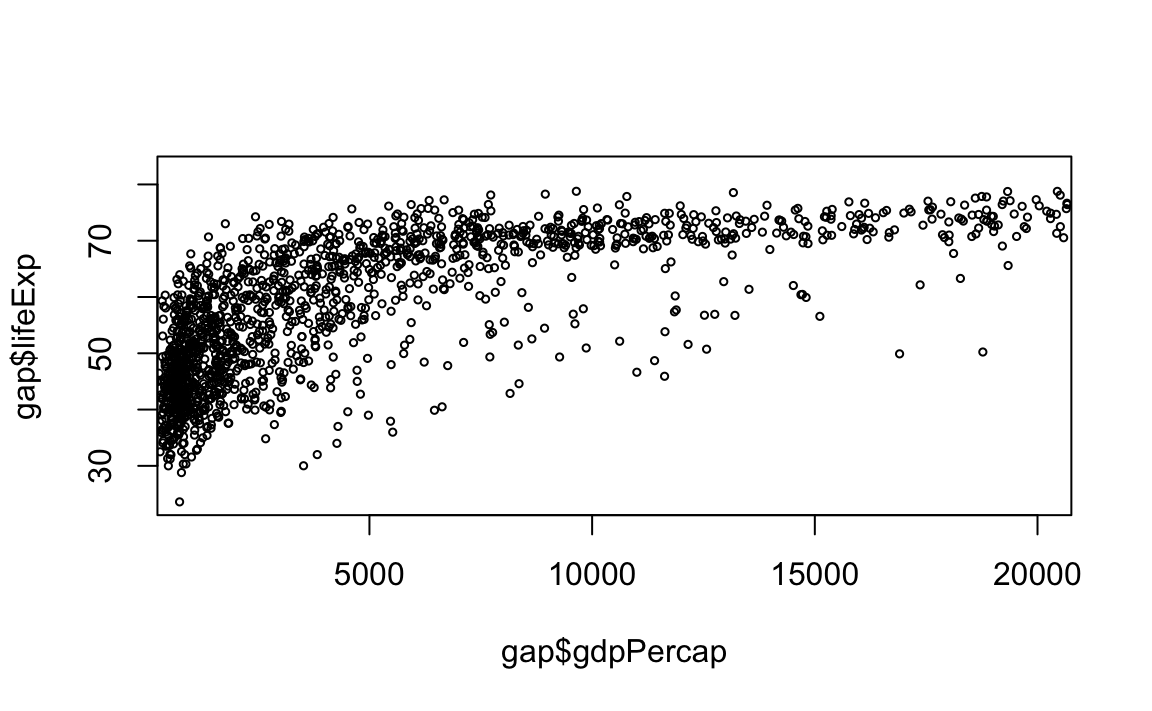
\includegraphics[width=0.7\linewidth]{site1_files/figure-latex/unnamed-chunk-275-4} 

}

\caption{ }\label{fig:unnamed-chunk-275}
\end{figure}

\subsection{Graphical parameters}\label{graphical-parameters}

We can change the points with a number of graphical options:

\begin{Shaded}
\begin{Highlighting}[]
\KeywordTok{plot}\NormalTok{(}\DataTypeTok{x=}\NormalTok{, }\DataTypeTok{y=}\NormalTok{, }\DataTypeTok{type=}\StringTok{""}\NormalTok{, }\DataTypeTok{col=}\StringTok{""}\NormalTok{, }\DataTypeTok{pch=}\NormalTok{, }\DataTypeTok{lty=}\NormalTok{, }\DataTypeTok{lwd=}\NormalTok{)}
\end{Highlighting}
\end{Shaded}

\begin{itemize}
\tightlist
\item
  Colors
\end{itemize}

\begin{Shaded}
\begin{Highlighting}[]
\KeywordTok{colors}\NormalTok{()[}\DecValTok{1}\OperatorTok{:}\DecValTok{20}\NormalTok{] }\CommentTok{# View first 20 elements of the color vector}
\CommentTok{#>  [1] "white"         "aliceblue"     "antiquewhite"  "antiquewhite1"}
\CommentTok{#>  [5] "antiquewhite2" "antiquewhite3" "antiquewhite4" "aquamarine"   }
\CommentTok{#>  [9] "aquamarine1"   "aquamarine2"   "aquamarine3"   "aquamarine4"  }
\CommentTok{#> [13] "azure"         "azure1"        "azure2"        "azure3"       }
\CommentTok{#> [17] "azure4"        "beige"         "bisque"        "bisque1"}
\KeywordTok{colors}\NormalTok{()[}\DecValTok{179}\NormalTok{] }\CommentTok{# View specific element of the color vector}
\CommentTok{#> [1] "gray26"}
\end{Highlighting}
\end{Shaded}

Another option:
\href{http://research.stowers-institute.org/efg/R/Color/Chart/ColorsChart1.jpg}{R
Color Infographic}

\begin{Shaded}
\begin{Highlighting}[]
\KeywordTok{plot}\NormalTok{(}\DataTypeTok{x =}\NormalTok{ gap}\OperatorTok{$}\NormalTok{gdpPercap, }\DataTypeTok{y =}\NormalTok{ gap}\OperatorTok{$}\NormalTok{lifeExp, }\DataTypeTok{type=}\StringTok{"p"}\NormalTok{, }\DataTypeTok{col=}\KeywordTok{colors}\NormalTok{()[}\DecValTok{145}\NormalTok{]) }\CommentTok{# or col="gold3"}
\KeywordTok{plot}\NormalTok{(}\DataTypeTok{x =}\NormalTok{ gap}\OperatorTok{$}\NormalTok{gdpPercap, }\DataTypeTok{y =}\NormalTok{ gap}\OperatorTok{$}\NormalTok{lifeExp, }\DataTypeTok{type=}\StringTok{"p"}\NormalTok{, }\DataTypeTok{col=}\StringTok{"seagreen4"}\NormalTok{) }\CommentTok{# or col=colors()[578]}
\end{Highlighting}
\end{Shaded}

\begin{figure}

{\centering 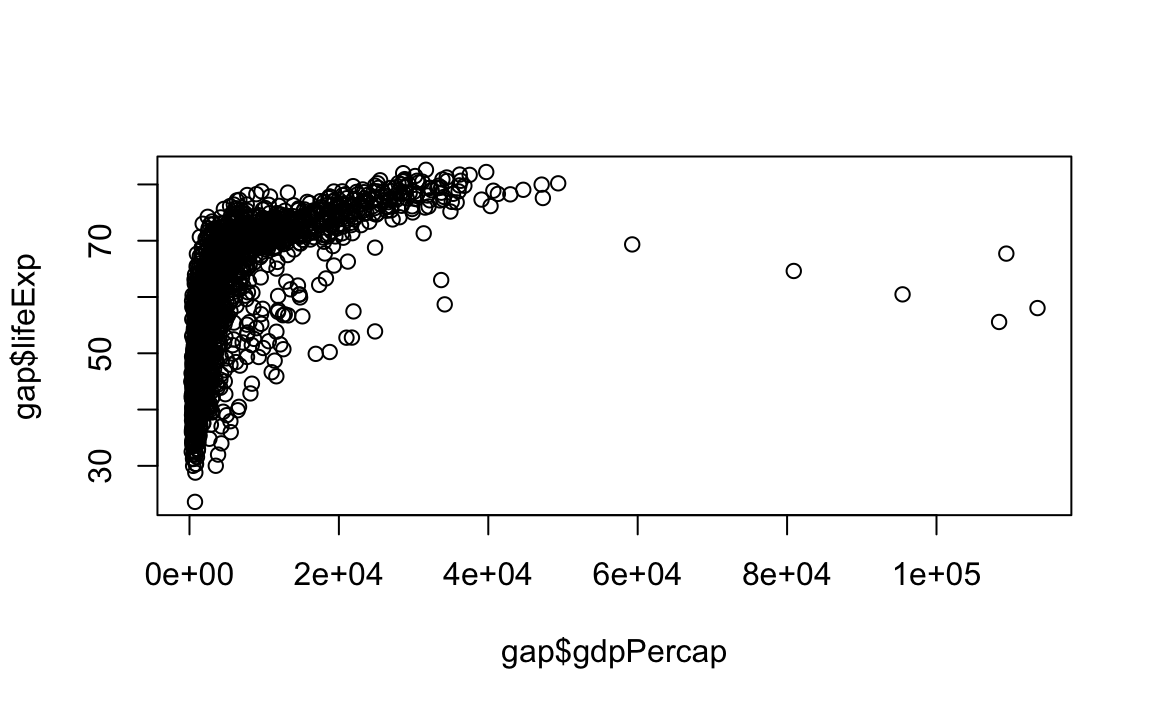
\includegraphics[width=0.7\linewidth]{site1_files/figure-latex/unnamed-chunk-278-1} 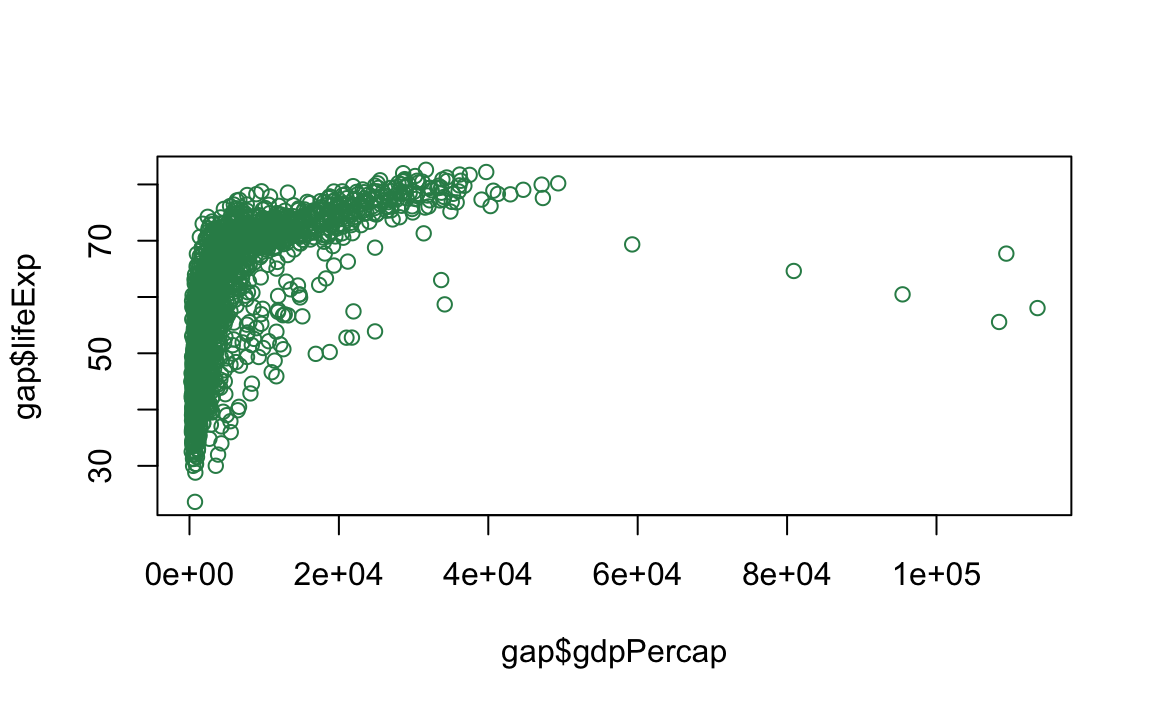
\includegraphics[width=0.7\linewidth]{site1_files/figure-latex/unnamed-chunk-278-2} 

}

\caption{ }\label{fig:unnamed-chunk-278}
\end{figure}

\begin{itemize}
\tightlist
\item
  Point Styles and Widths
\end{itemize}

\href{http://www.endmemo.com/program/R/pic/pchsymbols.png}{A Good
Reference}

\begin{Shaded}
\begin{Highlighting}[]
\CommentTok{# Change point style to crosses}
\KeywordTok{plot}\NormalTok{(}\DataTypeTok{x =}\NormalTok{ gap}\OperatorTok{$}\NormalTok{gdpPercap, }\DataTypeTok{y =}\NormalTok{ gap}\OperatorTok{$}\NormalTok{lifeExp, }\DataTypeTok{type=}\StringTok{"p"}\NormalTok{, }\DataTypeTok{pch=}\DecValTok{3}\NormalTok{) }
\CommentTok{# Change point style to filled squares}
\KeywordTok{plot}\NormalTok{(}\DataTypeTok{x =}\NormalTok{ gap}\OperatorTok{$}\NormalTok{gdpPercap, }\DataTypeTok{y =}\NormalTok{ gap}\OperatorTok{$}\NormalTok{lifeExp, }\DataTypeTok{type=}\StringTok{"p"}\NormalTok{,}\DataTypeTok{pch=}\DecValTok{15}\NormalTok{) }
\CommentTok{# Change point style to filled squares and increase point size to 3}
\KeywordTok{plot}\NormalTok{(}\DataTypeTok{x =}\NormalTok{ gap}\OperatorTok{$}\NormalTok{gdpPercap, }\DataTypeTok{y =}\NormalTok{ gap}\OperatorTok{$}\NormalTok{lifeExp, }\DataTypeTok{type=}\StringTok{"p"}\NormalTok{,}\DataTypeTok{pch=}\DecValTok{15}\NormalTok{, }\DataTypeTok{cex=}\DecValTok{3}\NormalTok{) }
\CommentTok{# Change point style to "w"}
\KeywordTok{plot}\NormalTok{(}\DataTypeTok{x =}\NormalTok{ gap}\OperatorTok{$}\NormalTok{gdpPercap, }\DataTypeTok{y =}\NormalTok{ gap}\OperatorTok{$}\NormalTok{lifeExp, }\DataTypeTok{type=}\StringTok{"p"}\NormalTok{, }\DataTypeTok{pch=}\StringTok{"w"}\NormalTok{)}
\CommentTok{# Change point style to "$" and increase point size to 2}
\KeywordTok{plot}\NormalTok{(}\DataTypeTok{x =}\NormalTok{ gap}\OperatorTok{$}\NormalTok{gdpPercap, }\DataTypeTok{y =}\NormalTok{ gap}\OperatorTok{$}\NormalTok{lifeExp, }\DataTypeTok{type=}\StringTok{"p"}\NormalTok{,}\DataTypeTok{pch=}\StringTok{"$"}\NormalTok{, }\DataTypeTok{cex=}\DecValTok{2}\NormalTok{) }
\end{Highlighting}
\end{Shaded}

\begin{figure}

{\centering 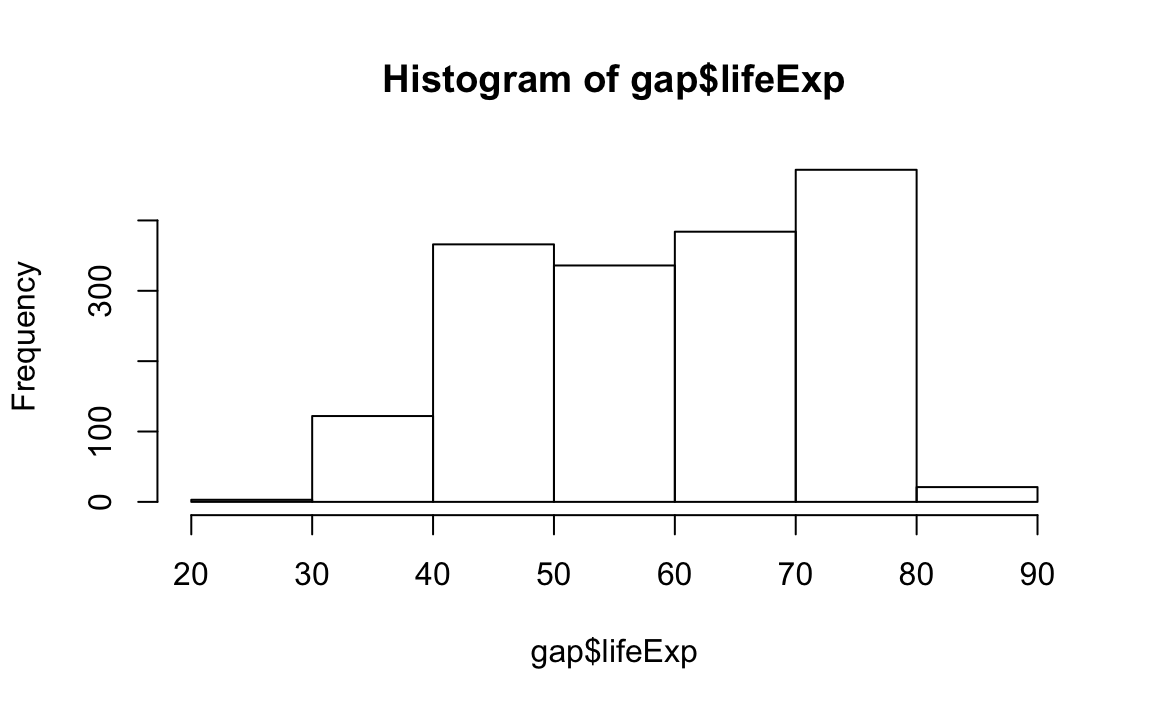
\includegraphics[width=0.7\linewidth]{site1_files/figure-latex/unnamed-chunk-279-1} 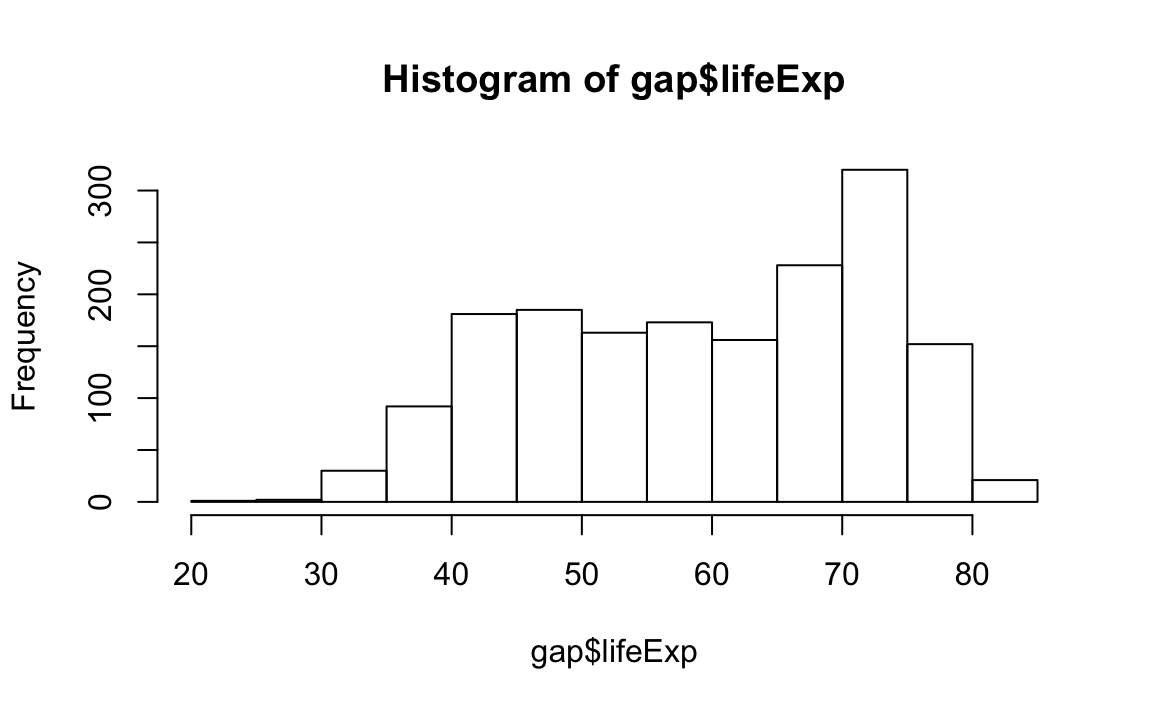
\includegraphics[width=0.7\linewidth]{site1_files/figure-latex/unnamed-chunk-279-2} 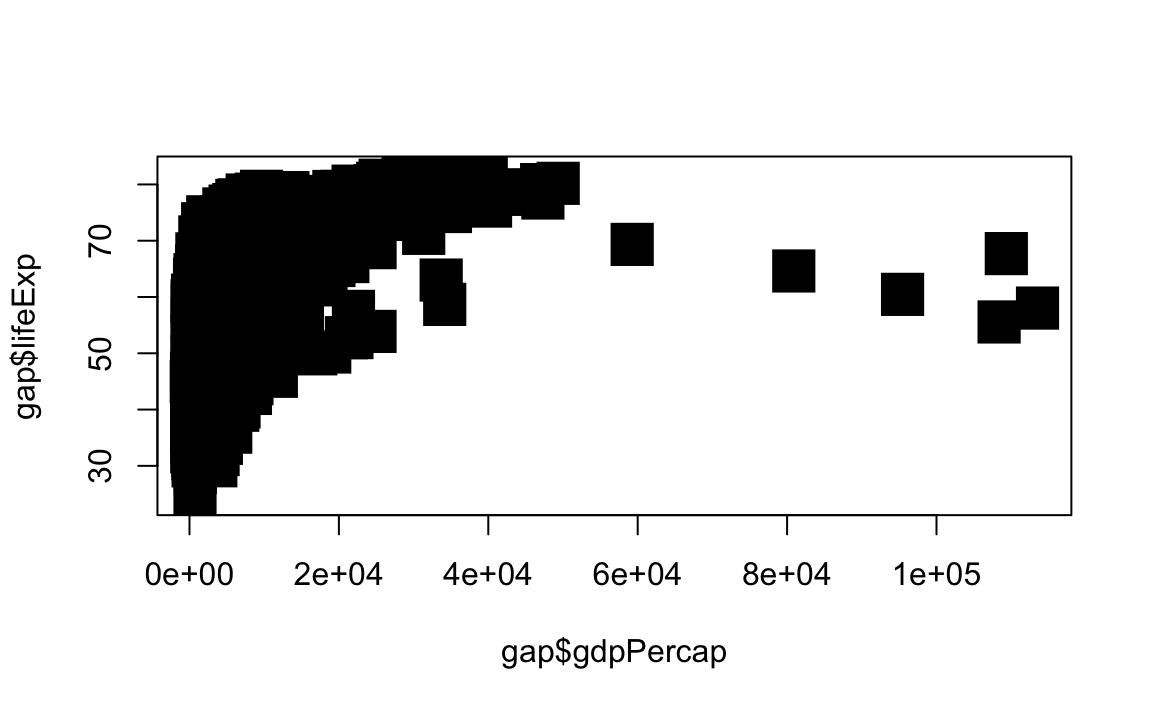
\includegraphics[width=0.7\linewidth]{site1_files/figure-latex/unnamed-chunk-279-3} 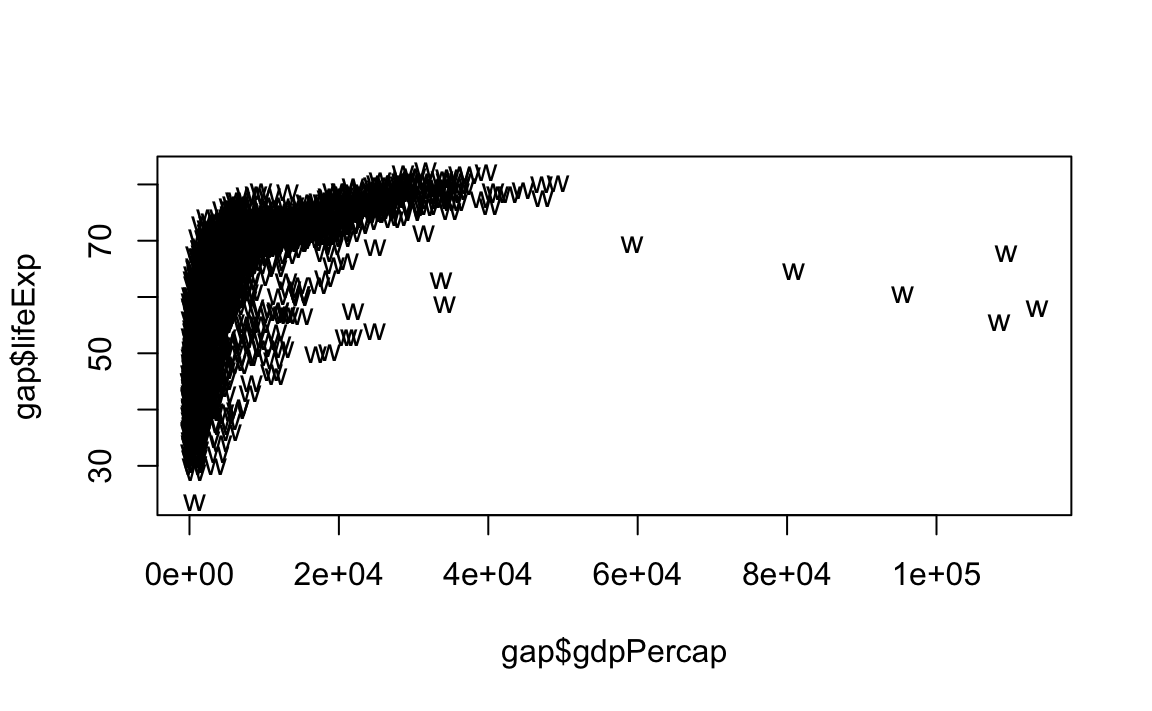
\includegraphics[width=0.7\linewidth]{site1_files/figure-latex/unnamed-chunk-279-4} 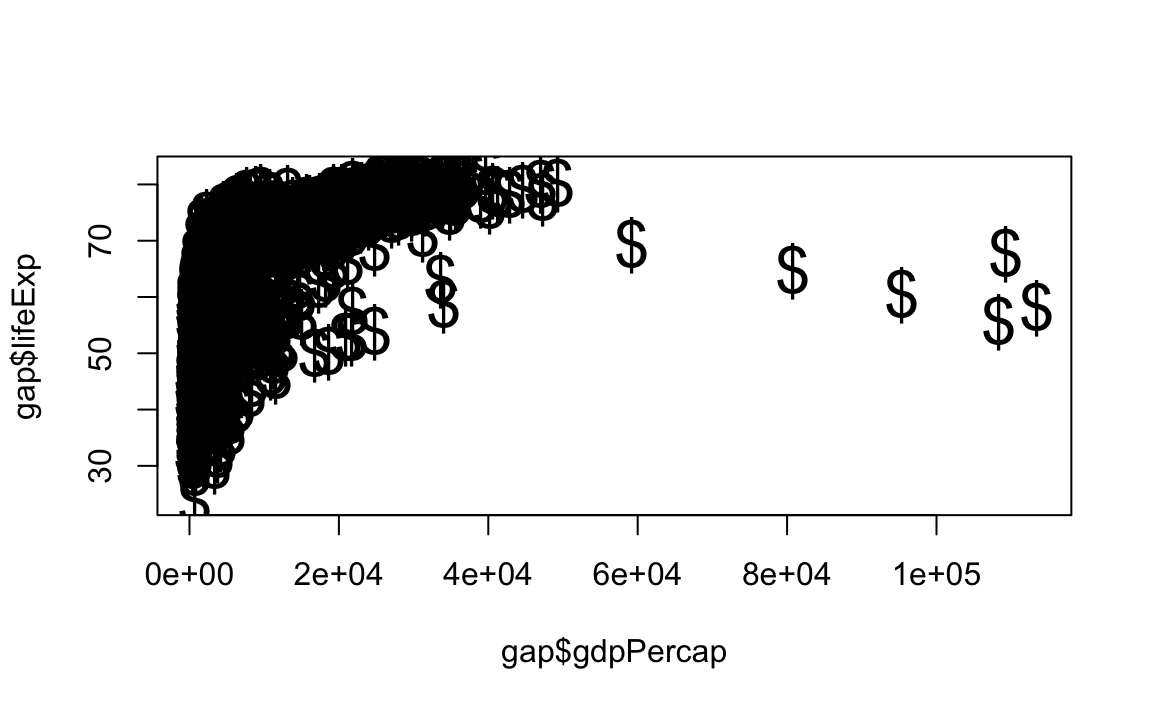
\includegraphics[width=0.7\linewidth]{site1_files/figure-latex/unnamed-chunk-279-5} 

}

\caption{ }\label{fig:unnamed-chunk-279}
\end{figure}

\begin{itemize}
\tightlist
\item
  Line Styles and Widths
\end{itemize}

\begin{Shaded}
\begin{Highlighting}[]
\CommentTok{# Line plot with solid line}
\KeywordTok{plot}\NormalTok{(}\DataTypeTok{x =}\NormalTok{ gap}\OperatorTok{$}\NormalTok{gdpPercap, }\DataTypeTok{y =}\NormalTok{ gap}\OperatorTok{$}\NormalTok{lifeExp, }\DataTypeTok{type=}\StringTok{"l"}\NormalTok{, }\DataTypeTok{lty=}\DecValTok{1}\NormalTok{)}
\CommentTok{# Line plot with medium dashed line}
\KeywordTok{plot}\NormalTok{(}\DataTypeTok{x =}\NormalTok{ gap}\OperatorTok{$}\NormalTok{gdpPercap, }\DataTypeTok{y =}\NormalTok{ gap}\OperatorTok{$}\NormalTok{lifeExp, }\DataTypeTok{type=}\StringTok{"l"}\NormalTok{, }\DataTypeTok{lty=}\DecValTok{2}\NormalTok{)}
\CommentTok{# Line plot with short dashed line}
\KeywordTok{plot}\NormalTok{(}\DataTypeTok{x =}\NormalTok{ gap}\OperatorTok{$}\NormalTok{gdpPercap, }\DataTypeTok{y =}\NormalTok{ gap}\OperatorTok{$}\NormalTok{lifeExp, }\DataTypeTok{type=}\StringTok{"l"}\NormalTok{, }\DataTypeTok{lty=}\DecValTok{3}\NormalTok{)}
\CommentTok{# Change line width to 2}
\KeywordTok{plot}\NormalTok{(}\DataTypeTok{x =}\NormalTok{ gap}\OperatorTok{$}\NormalTok{gdpPercap, }\DataTypeTok{y =}\NormalTok{ gap}\OperatorTok{$}\NormalTok{lifeExp, }\DataTypeTok{type=}\StringTok{"l"}\NormalTok{, }\DataTypeTok{lty=}\DecValTok{3}\NormalTok{, }\DataTypeTok{lwd=}\DecValTok{2}\NormalTok{)}
\CommentTok{# Change line width to 5}
\KeywordTok{plot}\NormalTok{(}\DataTypeTok{x =}\NormalTok{ gap}\OperatorTok{$}\NormalTok{gdpPercap, }\DataTypeTok{y =}\NormalTok{ gap}\OperatorTok{$}\NormalTok{lifeExp, }\DataTypeTok{type=}\StringTok{"l"}\NormalTok{,  }\DataTypeTok{lwd=}\DecValTok{5}\NormalTok{)}
\CommentTok{# Change line width to 10 and use dash-dot}
\KeywordTok{plot}\NormalTok{(}\DataTypeTok{x =}\NormalTok{ gap}\OperatorTok{$}\NormalTok{gdpPercap, }\DataTypeTok{y =}\NormalTok{ gap}\OperatorTok{$}\NormalTok{lifeExp, }\DataTypeTok{type=}\StringTok{"l"}\NormalTok{,  }\DataTypeTok{lty=}\DecValTok{4}\NormalTok{, }\DataTypeTok{lwd=}\DecValTok{10}\NormalTok{)}
\end{Highlighting}
\end{Shaded}

\begin{figure}

{\centering 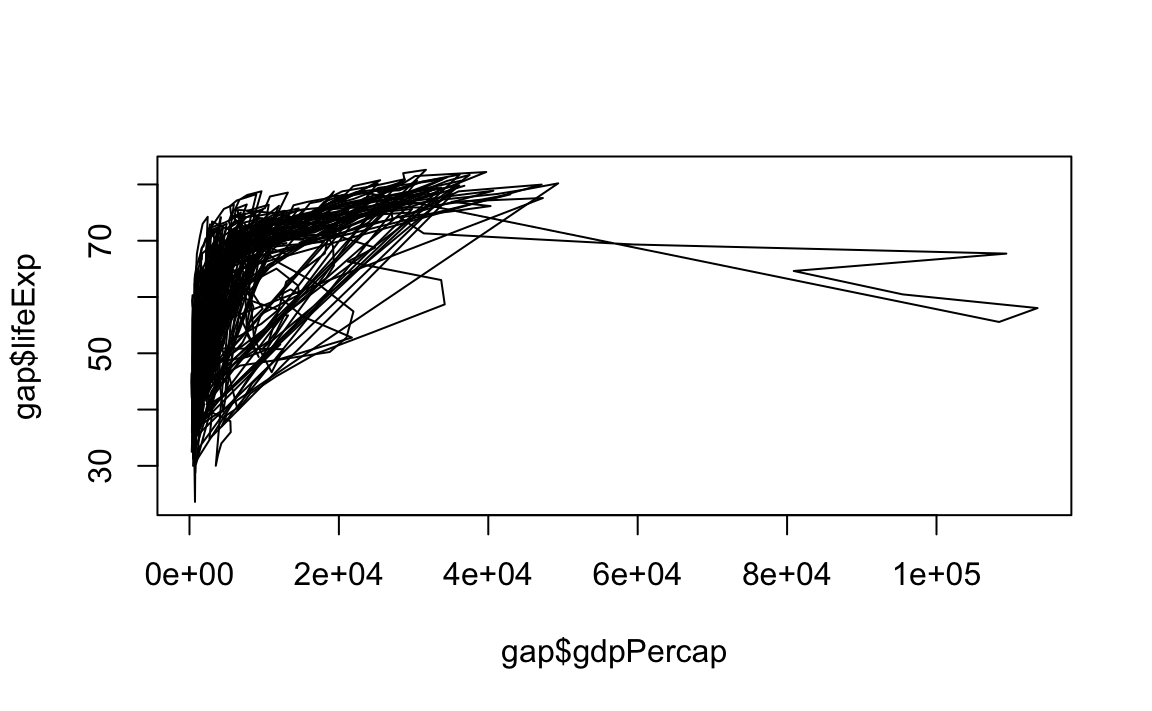
\includegraphics[width=0.7\linewidth]{site1_files/figure-latex/unnamed-chunk-280-1} 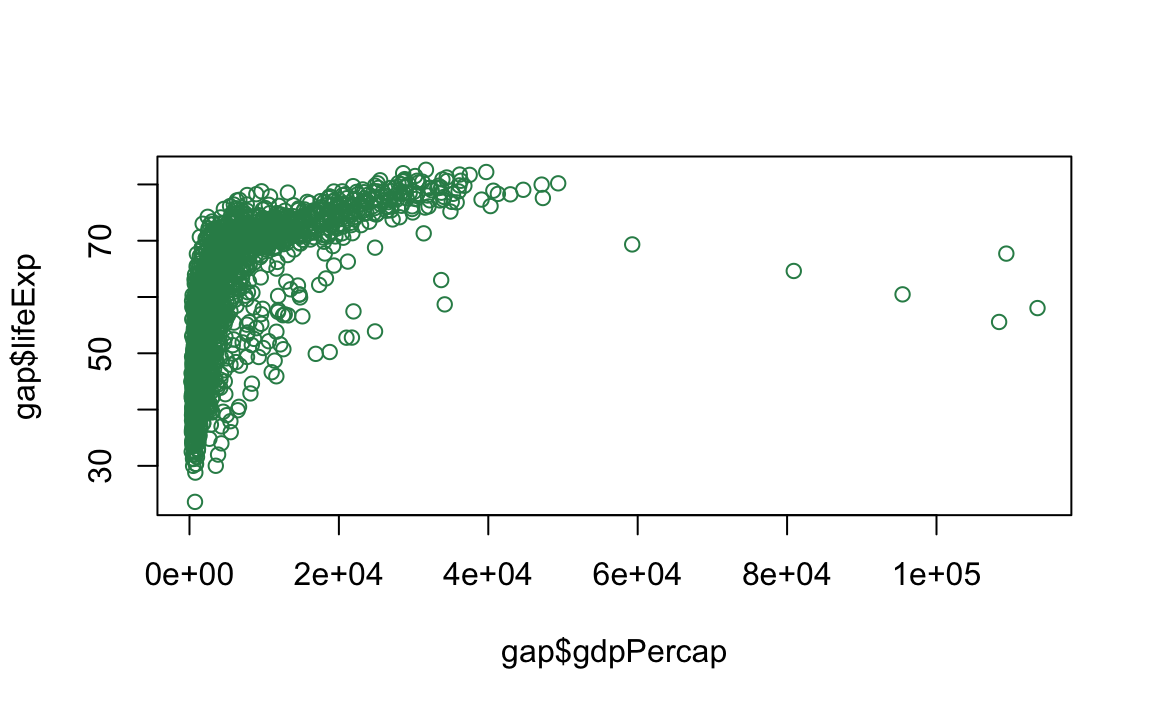
\includegraphics[width=0.7\linewidth]{site1_files/figure-latex/unnamed-chunk-280-2} 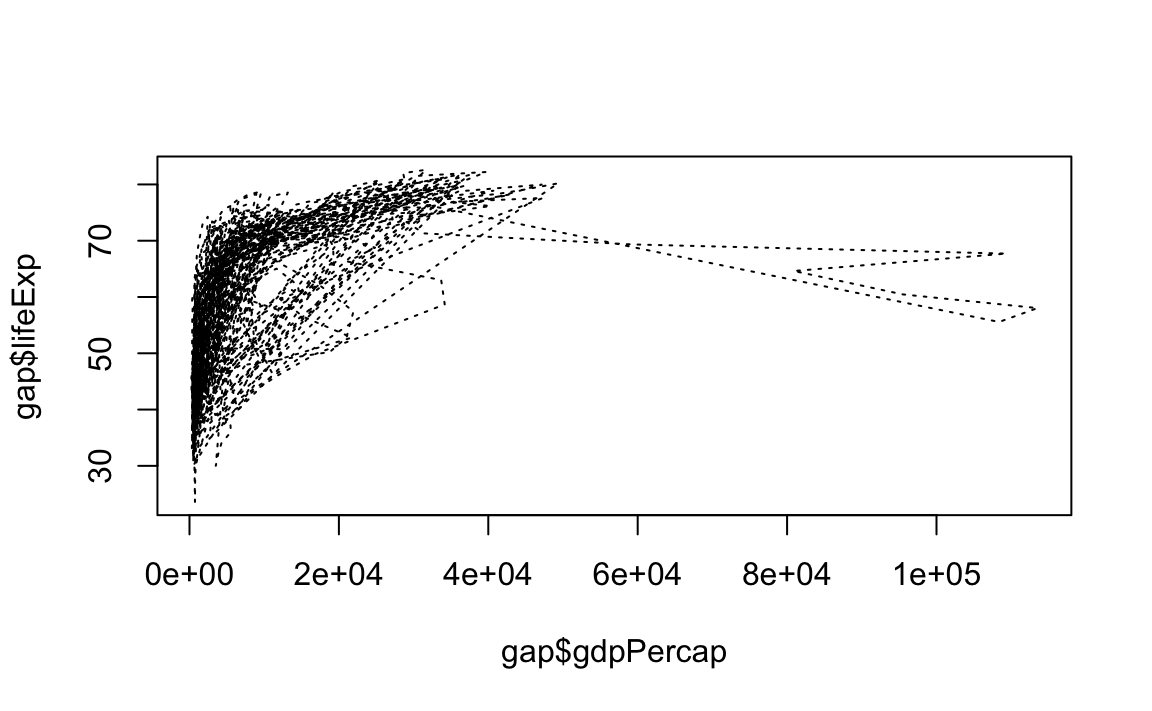
\includegraphics[width=0.7\linewidth]{site1_files/figure-latex/unnamed-chunk-280-3} 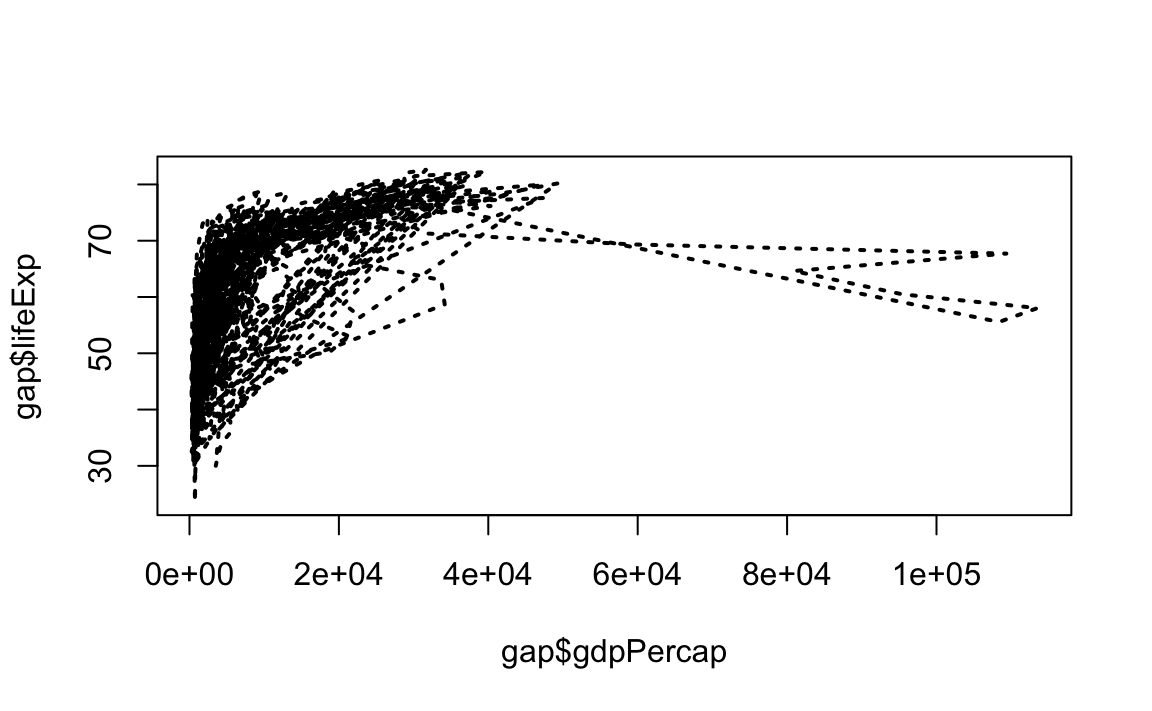
\includegraphics[width=0.7\linewidth]{site1_files/figure-latex/unnamed-chunk-280-4} 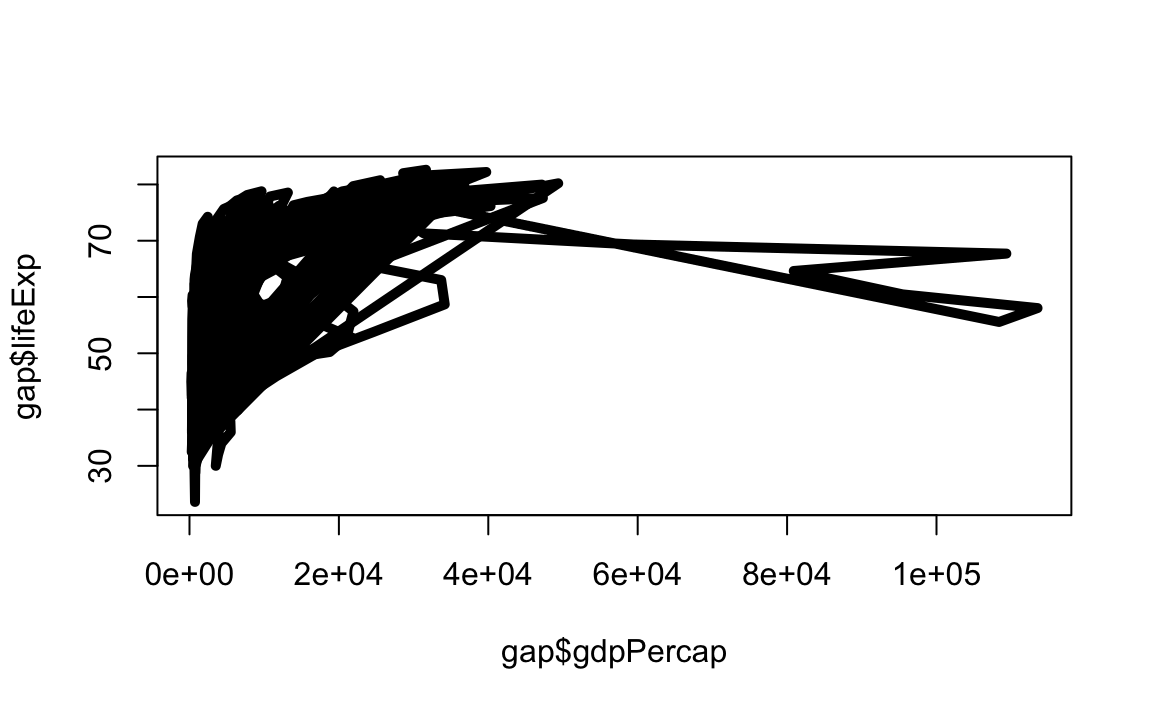
\includegraphics[width=0.7\linewidth]{site1_files/figure-latex/unnamed-chunk-280-5} 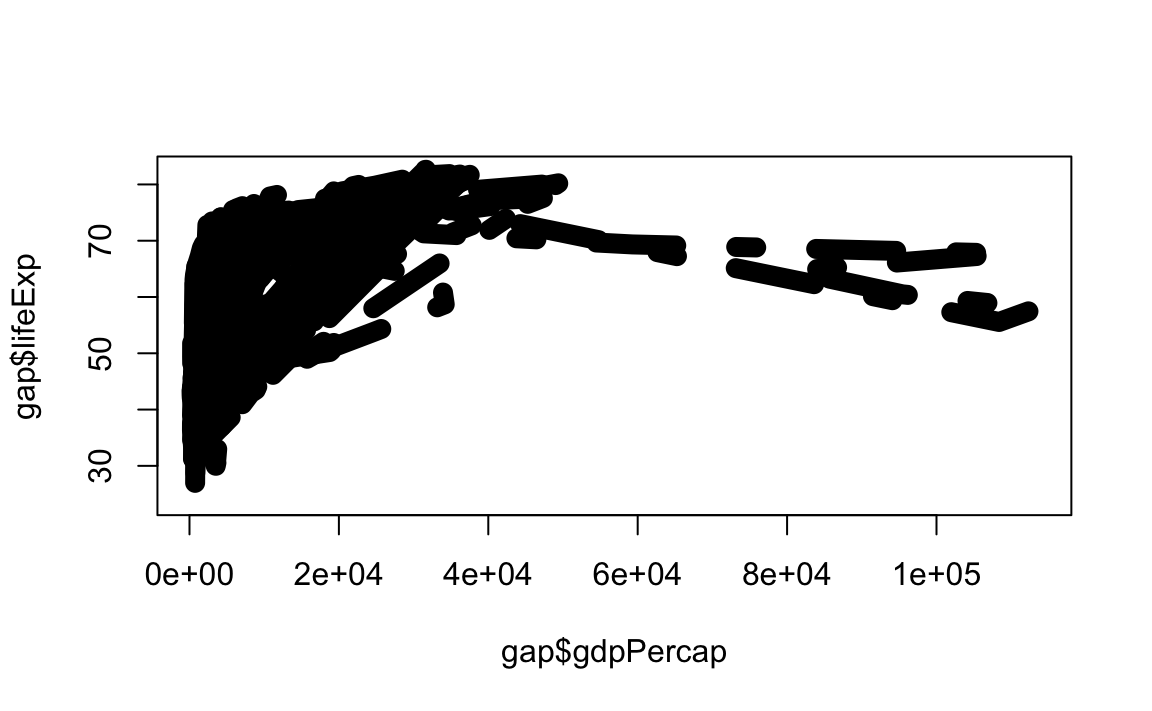
\includegraphics[width=0.7\linewidth]{site1_files/figure-latex/unnamed-chunk-280-6} 

}

\caption{ }\label{fig:unnamed-chunk-280}
\end{figure}

\subsection{Annotations, reference lines, and
legends}\label{annotations-reference-lines-and-legends}

\begin{itemize}
\tightlist
\item
  Text
\end{itemize}

We can add text to an arbitrary point on the graph like this:

\begin{Shaded}
\begin{Highlighting}[]
\CommentTok{# plot the line first}
\KeywordTok{plot}\NormalTok{(}\DataTypeTok{x =}\NormalTok{ gap}\OperatorTok{$}\NormalTok{gdpPercap, }\DataTypeTok{y =}\NormalTok{ gap}\OperatorTok{$}\NormalTok{lifeExp, }\DataTypeTok{type=}\StringTok{"p"}\NormalTok{)}
\CommentTok{# now add the label}
\KeywordTok{text}\NormalTok{(}\DataTypeTok{x=}\DecValTok{40000}\NormalTok{, }\DataTypeTok{y=}\DecValTok{50}\NormalTok{, }\DataTypeTok{labels=}\StringTok{"Evens Out"}\NormalTok{, }\DataTypeTok{cex =}\NormalTok{ .}\DecValTok{75}\NormalTok{)}
\end{Highlighting}
\end{Shaded}

\begin{figure}

{\centering 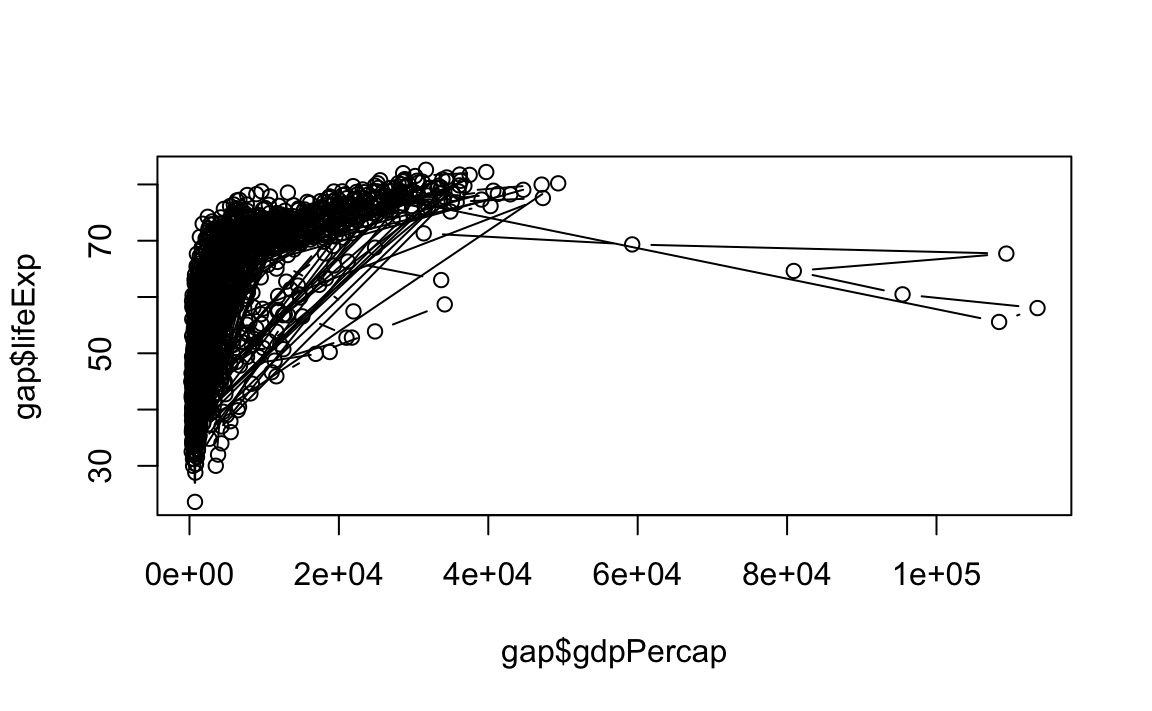
\includegraphics[width=0.7\linewidth]{site1_files/figure-latex/unnamed-chunk-281-1} 

}

\caption{ }\label{fig:unnamed-chunk-281}
\end{figure}

We can also add labels for every point by passing in a vector of text:

\begin{Shaded}
\begin{Highlighting}[]
\CommentTok{# first randomly select rows for a smaller gapaset}
\KeywordTok{library}\NormalTok{(dplyr)}
\NormalTok{small <-}\StringTok{ }\NormalTok{gap }\OperatorTok\StringTok{ }\KeywordTok{sample_n}\NormalTok{(}\DecValTok{100}\NormalTok{)}

\CommentTok{# plot the line first}
\KeywordTok{plot}\NormalTok{(}\DataTypeTok{x =}\NormalTok{ small}\OperatorTok{$}\NormalTok{gdpPercap, }\DataTypeTok{y =}\NormalTok{ small}\OperatorTok{$}\NormalTok{lifeExp, }\DataTypeTok{type=}\StringTok{"p"}\NormalTok{)}
\CommentTok{# now add the label}
\KeywordTok{text}\NormalTok{(}\DataTypeTok{x =}\NormalTok{ small}\OperatorTok{$}\NormalTok{gdpPercap, }\DataTypeTok{y =}\NormalTok{ small}\OperatorTok{$}\NormalTok{lifeExp, }\DataTypeTok{labels =}\NormalTok{ small}\OperatorTok{$}\NormalTok{country)}
\end{Highlighting}
\end{Shaded}

\begin{figure}

{\centering 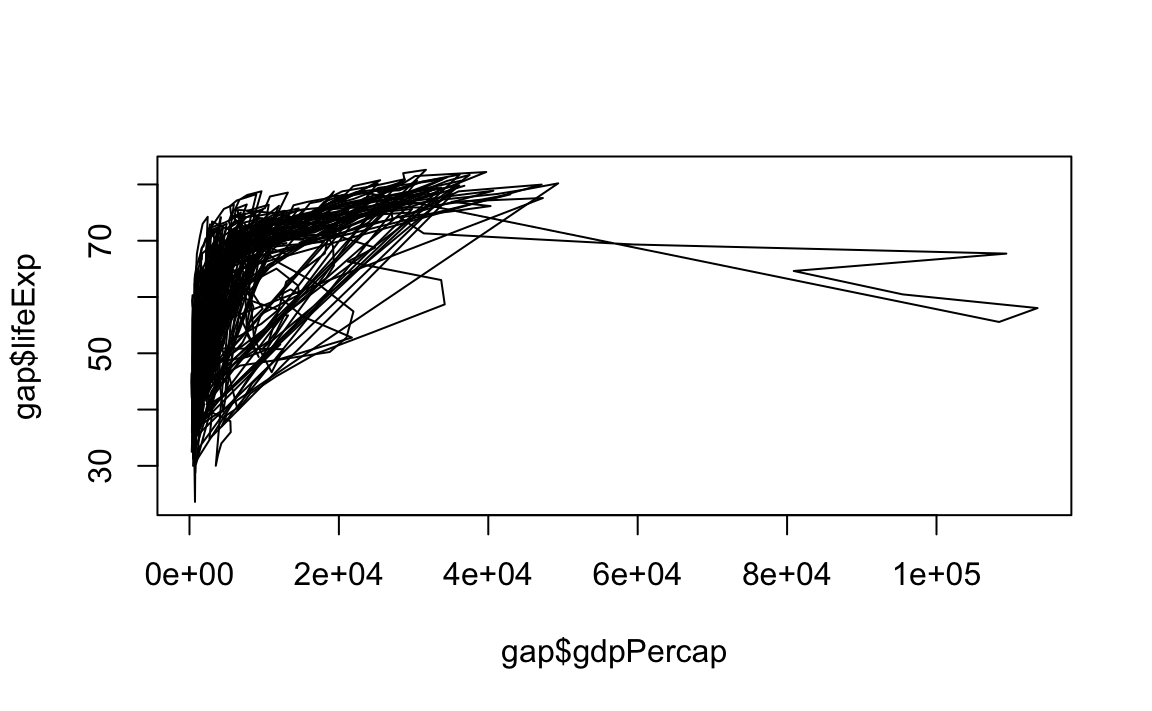
\includegraphics[width=0.7\linewidth]{site1_files/figure-latex/unnamed-chunk-282-1} 

}

\caption{ }\label{fig:unnamed-chunk-282}
\end{figure}

\begin{itemize}
\tightlist
\item
  Reference Lines
\end{itemize}

\begin{Shaded}
\begin{Highlighting}[]
\CommentTok{# plot the line}
\KeywordTok{plot}\NormalTok{(}\DataTypeTok{x =}\NormalTok{ gap}\OperatorTok{$}\NormalTok{gdpPercap, }\DataTypeTok{y =}\NormalTok{ gap}\OperatorTok{$}\NormalTok{lifeExp, }\DataTypeTok{type=}\StringTok{"p"}\NormalTok{)}
\CommentTok{# now the guides}
\KeywordTok{abline}\NormalTok{(}\DataTypeTok{v=}\DecValTok{40000}\NormalTok{, }\DataTypeTok{h=}\DecValTok{75}\NormalTok{, }\DataTypeTok{lty=}\DecValTok{2}\NormalTok{)}
\end{Highlighting}
\end{Shaded}

\begin{figure}

{\centering 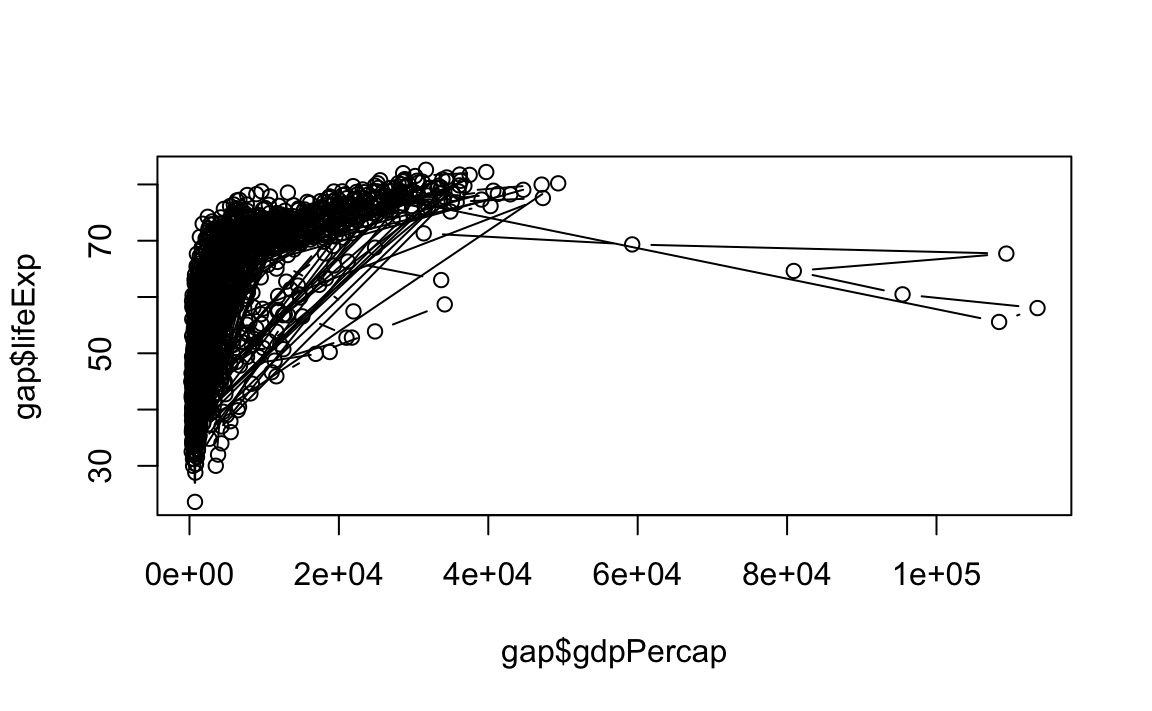
\includegraphics[width=0.7\linewidth]{site1_files/figure-latex/unnamed-chunk-283-1} 

}

\caption{ }\label{fig:unnamed-chunk-283}
\end{figure}

\section{ggplot2}\label{ggplot2}

Setup:

\begin{Shaded}
\begin{Highlighting}[]
\KeywordTok{library}\NormalTok{(ggplot2)}
\NormalTok{gap <-}\StringTok{ }\KeywordTok{read.csv}\NormalTok{(}\StringTok{"data/gapminder-FiveYearData.csv"}\NormalTok{, }\DataTypeTok{stringsAsFactors =}\NormalTok{ F)}
\end{Highlighting}
\end{Shaded}

\subsubsection*{Why ggplot?}\label{why-ggplot}
\addcontentsline{toc}{subsubsection}{Why ggplot?}

\begin{itemize}
\tightlist
\item
  More elegant \& compact code than with base graphics
\item
  More aesthetically pleasing defaults than lattice
\item
  Very powerful for exploratory data analysis
\item
  Follows a grammar, just like any language.
\item
  It defines basic components that make up a sentence. In this case, the
  grammar defines components in a plot.
\item
  \emph{G}rammar of \emph{g}raphics originally coined by Lee Wilkinson
\end{itemize}

\subsection{Grammar}\label{grammar}

The general call for ggplot2 looks like this:

\begin{Shaded}
\begin{Highlighting}[]
\KeywordTok{ggplot}\NormalTok{(}\DataTypeTok{data=}\NormalTok{, }\KeywordTok{aes}\NormalTok{(}\DataTypeTok{x=}\NormalTok{, }\DataTypeTok{y=}\NormalTok{), }\DataTypeTok{color=}\NormalTok{, }\DataTypeTok{size=}\NormalTok{,) }\OperatorTok{+}\StringTok{ }\KeywordTok{geom_xxxx}\NormalTok{()}\OperatorTok{+}\KeywordTok{geom_yyyy}\NormalTok{()}
\end{Highlighting}
\end{Shaded}

The \emph{grammar} involves some basic components:

\begin{enumerate}
\def\labelenumi{\arabic{enumi}.}
\tightlist
\item
  \textbf{Data}: a data.frame
\item
  \textbf{Aes}thetics: How your data are represented visually, aka
  ``mapping''. Which variables are shown on x, y axes, as well as color,
  size, shape, etc.
\item
  \textbf{Geom}etry: The geometric objects in a plot. points, lines,
  polygons, etc.
\end{enumerate}

The key to understanding \texttt{ggplot2} is thinking about a figure in
layers: just like you might do in an image editing program like
Photoshop, Illustrator, or Inkscape.

Let's look at an example:

\begin{verbatim}
ggplot(data = gap, aes(x = gdpPercap, y = lifeExp)) +
  geom_point()
\end{verbatim}

So the first thing we do is call the \texttt{ggplot} function. This
function lets R know that we're creating a new plot, and any of the
arguments we give the ggplot function are the global options for the
plot: they apply to all layers on the plot.

We've passed in two arguments to \texttt{ggplot}. First, we tell
\texttt{ggplot} what \textbf{\texttt{data}} we want to show on our
figure, in this example the \texttt{gapminder} data we read in earlier.

For the second argument we passed in the \textbf{\texttt{aes}} function,
which tells \texttt{ggplot} how variables in the data map to aesthetic
properties of the figure, in this case the x and y locations. Here we
told \texttt{ggplot} we want to plot the \texttt{lifeExp} column of the
gapminder data frame on the x-axis, and the \texttt{gdpPercap} column on
the y-axis.

Notice that we didn't need to explicitly pass \texttt{aes} these columns
(e.g. \texttt{x\ =\ gapminder{[},\ "lifeExp""{]})}, this is because
\texttt{ggplot} is smart enough to know to look in the data for that
column!

By itself, the call to \texttt{ggplot} isn't enough to draw a figure:

\begin{Shaded}
\begin{Highlighting}[]
\KeywordTok{ggplot}\NormalTok{(}\DataTypeTok{data =}\NormalTok{ gap, }\KeywordTok{aes}\NormalTok{(}\DataTypeTok{x =}\NormalTok{ gdpPercap, }\DataTypeTok{y =}\NormalTok{ lifeExp))}
\end{Highlighting}
\end{Shaded}

We need to tell \texttt{ggplot} how we want to visually represent the
data, which we do by adding a new \textbf{\texttt{geom}} layer. In our
example, we used \texttt{geom\_point}, which tells ggplot we want to
visually represent the relationship between x and y as a scatterplot of
points:

\begin{Shaded}
\begin{Highlighting}[]
\KeywordTok{ggplot}\NormalTok{(}\DataTypeTok{data =}\NormalTok{ gap, }\KeywordTok{aes}\NormalTok{(}\DataTypeTok{x =}\NormalTok{ gdpPercap, }\DataTypeTok{y =}\NormalTok{ lifeExp)) }\OperatorTok{+}\StringTok{ }
\StringTok{  }\KeywordTok{geom_point}\NormalTok{()}

\CommentTok{# same as}
\CommentTok{# my_plot <- ggplot(data = gap, aes(x = gdpPercap, y = lifeExp))}
\CommentTok{# my_plot + geom_point()}
\end{Highlighting}
\end{Shaded}

\begin{center}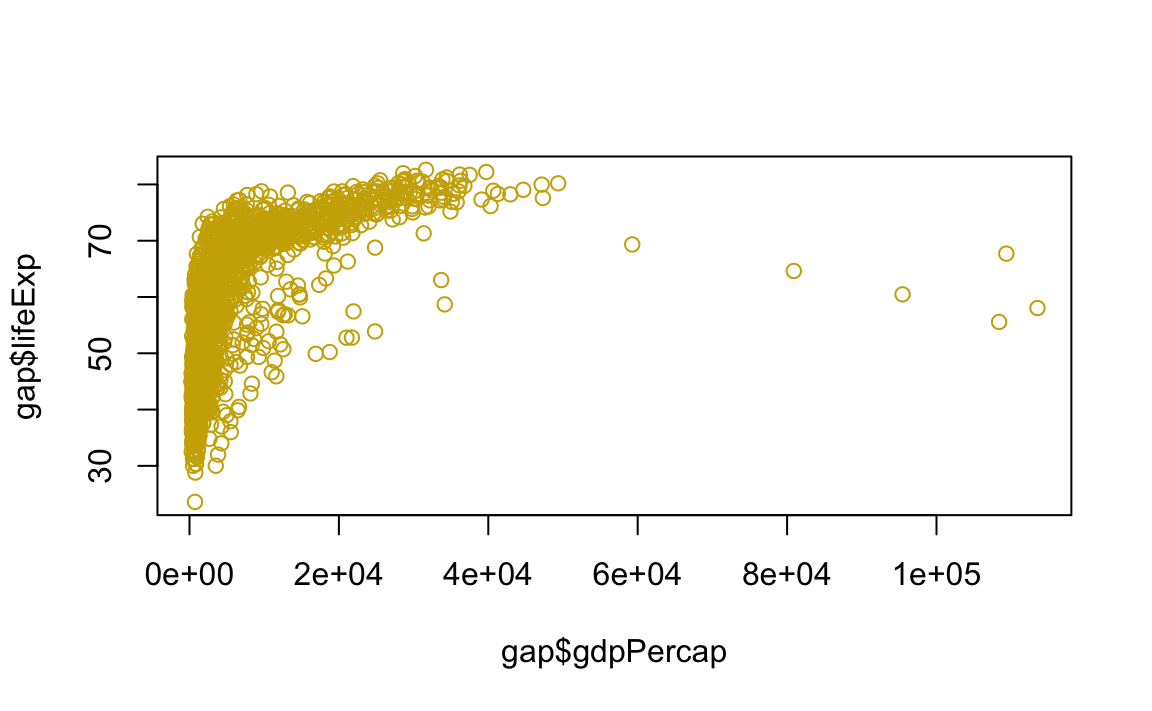
\includegraphics[width=0.7\linewidth]{site1_files/figure-latex/unnamed-chunk-288-1} \end{center}

\subsubsection*{Challenge 1}\label{challenge-1}
\addcontentsline{toc}{subsubsection}{Challenge 1}

Modify the example so that the figure visualise how life expectancy has
changed over time:

Hint: the gapminder dataset has a column called \texttt{year}, which
should appear on the x-axis.

\begin{Shaded}
\begin{Highlighting}[]
\CommentTok{# YOUR CODE HERE}
\end{Highlighting}
\end{Shaded}

\subsection{\texorpdfstring{Anatomy of
\texttt{aes}}{Anatomy of aes}}\label{anatomy-of-aes}

In the previous examples and challenge we've used the \texttt{aes}
function to tell the scatterplot \texttt{geom} about the \textbf{x} and
\textbf{y} locations of each point. Another aesthetic property we can
modify is the point \textbf{color}.

\begin{Shaded}
\begin{Highlighting}[]
\KeywordTok{ggplot}\NormalTok{(}\DataTypeTok{data =}\NormalTok{ gap, }\KeywordTok{aes}\NormalTok{(}\DataTypeTok{x =}\NormalTok{ gdpPercap, }\DataTypeTok{y =}\NormalTok{ lifeExp, }\DataTypeTok{color=}\NormalTok{continent)) }\OperatorTok{+}\StringTok{ }
\StringTok{  }\KeywordTok{geom_point}\NormalTok{()}
\end{Highlighting}
\end{Shaded}

\begin{center}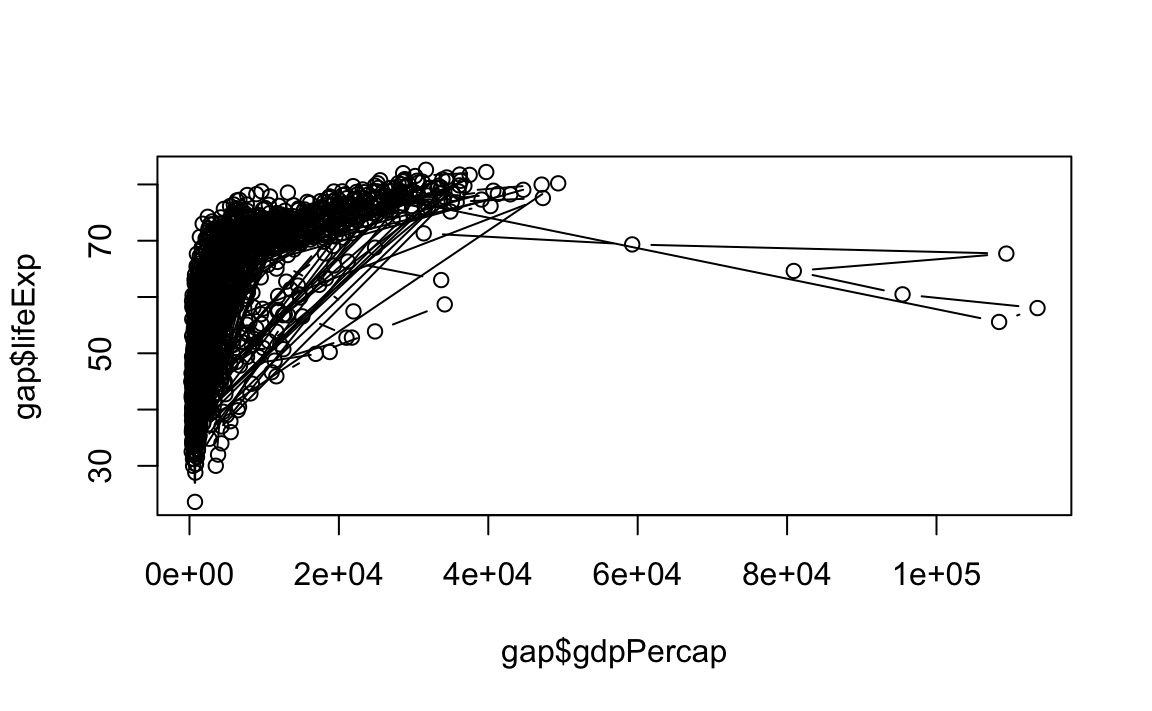
\includegraphics[width=0.7\linewidth]{site1_files/figure-latex/unnamed-chunk-290-1} \end{center}

Normally, specifying options like \texttt{color="red"} or
\texttt{size=10} for a given layer results in its contents being red and
quite large. Inside the \texttt{aes()} function, however, these
arguments are given entire variables whose values will then be displayed
using different realizations of that aesthetic.

\textbf{Color} isn't the only aesthetic argument we can set to display
variation in the data. We can also vary by shape, size, etc.

\begin{Shaded}
\begin{Highlighting}[]
\KeywordTok{ggplot}\NormalTok{(}\DataTypeTok{data=}\NormalTok{, }\KeywordTok{aes}\NormalTok{(}\DataTypeTok{x=}\NormalTok{, }\DataTypeTok{y=}\NormalTok{, }\DataTypeTok{by =}\NormalTok{, }\DataTypeTok{color=}\NormalTok{, }\DataTypeTok{linetype=}\NormalTok{, }\DataTypeTok{shape=}\NormalTok{, }\DataTypeTok{size=}\NormalTok{))}
\end{Highlighting}
\end{Shaded}

\subsection{Layers}\label{layers}

In the previous challenge, you plotted \texttt{lifExp} over time. Using
a scatterplot probably isn't the best for visualising change over time.
Instead, let's tell \texttt{ggplot} to visualise the data as a line
plot:

\begin{Shaded}
\begin{Highlighting}[]
\KeywordTok{ggplot}\NormalTok{(}\DataTypeTok{data =}\NormalTok{ gap, }\KeywordTok{aes}\NormalTok{(}\DataTypeTok{x=}\NormalTok{year, }\DataTypeTok{y=}\NormalTok{lifeExp, }\DataTypeTok{by=}\NormalTok{country, }\DataTypeTok{color=}\NormalTok{continent)) }\OperatorTok{+}\StringTok{ }
\StringTok{  }\KeywordTok{geom_line}\NormalTok{()}
\end{Highlighting}
\end{Shaded}

\begin{center}\includegraphics[width=0.7\linewidth]{site1_files/figure-latex/unnamed-chunk-292-1} \end{center}

Instead of adding a \texttt{geom\_point} layer, we've added a
\texttt{geom\_line} layer. We've also added the \textbf{by} aesthetic,
which tells ggplot to draw a line for each country.

But what if we want to visualise both lines and points on the plot? We
can simply add another layer to the plot:

\begin{Shaded}
\begin{Highlighting}[]
\KeywordTok{ggplot}\NormalTok{(}\DataTypeTok{data =}\NormalTok{ gap, }\KeywordTok{aes}\NormalTok{(}\DataTypeTok{x=}\NormalTok{year, }\DataTypeTok{y=}\NormalTok{lifeExp, }\DataTypeTok{by=}\NormalTok{country, }\DataTypeTok{color=}\NormalTok{continent)) }\OperatorTok{+}\StringTok{ }
\StringTok{  }\KeywordTok{geom_line}\NormalTok{() }\OperatorTok{+}\StringTok{ }
\StringTok{  }\KeywordTok{geom_point}\NormalTok{()}
\end{Highlighting}
\end{Shaded}

\begin{center}\includegraphics[width=0.7\linewidth]{site1_files/figure-latex/unnamed-chunk-293-1} \end{center}

It's important to note that each layer is drawn on top of the previous
layer. In this example, the points have been drawn on top of the lines.
Here's a demonstration:

\begin{Shaded}
\begin{Highlighting}[]
\KeywordTok{ggplot}\NormalTok{(}\DataTypeTok{data =}\NormalTok{ gap, }\KeywordTok{aes}\NormalTok{(}\DataTypeTok{x=}\NormalTok{year, }\DataTypeTok{y=}\NormalTok{lifeExp, }\DataTypeTok{by=}\NormalTok{country)) }\OperatorTok{+}\StringTok{ }
\StringTok{  }\KeywordTok{geom_line}\NormalTok{(}\KeywordTok{aes}\NormalTok{(}\DataTypeTok{color=}\NormalTok{continent)) }\OperatorTok{+}\StringTok{ }
\StringTok{  }\KeywordTok{geom_point}\NormalTok{()}
\end{Highlighting}
\end{Shaded}

\begin{center}\includegraphics[width=0.7\linewidth]{site1_files/figure-latex/unnamed-chunk-294-1} \end{center}

In this example, the aesthetic mapping of \textbf{color} has been moved
from the global plot options in ggplot to the \texttt{geom\_line} layer
so it no longer applies to the points. Now we can clearly see that the
points are drawn on top of the lines.

\subsubsection*{Challenge 2}\label{challenge-2}
\addcontentsline{toc}{subsubsection}{Challenge 2}

Switch the order of the point and line layers from the previous example.
What happened?

\subsection{Labels}\label{labels-1}

Labels are considered to be their own layers in ggplot.

\begin{Shaded}
\begin{Highlighting}[]
\CommentTok{# add x and y axis labels}
\KeywordTok{ggplot}\NormalTok{(}\DataTypeTok{data =}\NormalTok{ gap, }\KeywordTok{aes}\NormalTok{(}\DataTypeTok{x =}\NormalTok{ gdpPercap, }\DataTypeTok{y =}\NormalTok{ lifeExp, }\DataTypeTok{color=}\NormalTok{continent)) }\OperatorTok{+}\StringTok{ }
\StringTok{  }\KeywordTok{geom_point}\NormalTok{() }\OperatorTok{+}\StringTok{ }
\StringTok{  }\KeywordTok{xlab}\NormalTok{(}\StringTok{"GDP per capita"}\NormalTok{) }\OperatorTok{+}\StringTok{ }
\StringTok{  }\KeywordTok{ylab}\NormalTok{(}\StringTok{"Life Expectancy"}\NormalTok{) }\OperatorTok{+}\StringTok{ }
\StringTok{  }\KeywordTok{ggtitle}\NormalTok{(}\StringTok{"My fancy graph"}\NormalTok{)}
\end{Highlighting}
\end{Shaded}

\begin{center}\includegraphics[width=0.7\linewidth]{site1_files/figure-latex/unnamed-chunk-295-1} \end{center}

So are scales:

\begin{Shaded}
\begin{Highlighting}[]
\CommentTok{# limit x axis from 1,000 to 20,000}
\KeywordTok{ggplot}\NormalTok{(}\DataTypeTok{data =}\NormalTok{ gap, }\KeywordTok{aes}\NormalTok{(}\DataTypeTok{x =}\NormalTok{ gdpPercap, }\DataTypeTok{y =}\NormalTok{ lifeExp, }\DataTypeTok{color=}\NormalTok{continent)) }\OperatorTok{+}\StringTok{ }
\StringTok{  }\KeywordTok{geom_point}\NormalTok{() }\OperatorTok{+}\StringTok{ }
\StringTok{  }\KeywordTok{xlab}\NormalTok{(}\StringTok{"GDP per capita"}\NormalTok{) }\OperatorTok{+}\StringTok{ }
\StringTok{  }\KeywordTok{ylab}\NormalTok{(}\StringTok{"Life Expectancy"}\NormalTok{) }\OperatorTok{+}\StringTok{ }
\StringTok{  }\KeywordTok{ggtitle}\NormalTok{(}\StringTok{"My fancy graph"}\NormalTok{) }\OperatorTok{+}\StringTok{ }
\StringTok{  }\KeywordTok{xlim}\NormalTok{(}\DecValTok{1000}\NormalTok{, }\DecValTok{20000}\NormalTok{)}
\CommentTok{#> Warning: Removed 515 rows containing missing values (geom_point).}
\end{Highlighting}
\end{Shaded}

\begin{center}\includegraphics[width=0.7\linewidth]{site1_files/figure-latex/unnamed-chunk-296-1} \end{center}

\subsection{Transformations and Stats}\label{transformations-and-stats}

\texttt{ggplot} also makes it easy to overlay statistical models over
the data. To demonstrate we'll go back to an earlier example:

\begin{Shaded}
\begin{Highlighting}[]
\KeywordTok{ggplot}\NormalTok{(}\DataTypeTok{data =}\NormalTok{ gap, }\KeywordTok{aes}\NormalTok{(}\DataTypeTok{x =}\NormalTok{ gdpPercap, }\DataTypeTok{y =}\NormalTok{ lifeExp, }\DataTypeTok{color=}\NormalTok{continent)) }\OperatorTok{+}\StringTok{ }
\StringTok{  }\KeywordTok{geom_point}\NormalTok{()}
\end{Highlighting}
\end{Shaded}

\begin{center}\includegraphics[width=0.7\linewidth]{site1_files/figure-latex/unnamed-chunk-297-1} \end{center}

We can change the scale of units on the x axis using the \texttt{scale}
functions. These control the mapping between the data values and visual
values of an aesthetic.

\begin{Shaded}
\begin{Highlighting}[]
\KeywordTok{ggplot}\NormalTok{(}\DataTypeTok{data =}\NormalTok{ gap, }\KeywordTok{aes}\NormalTok{(}\DataTypeTok{x =}\NormalTok{ gdpPercap, }\DataTypeTok{y =}\NormalTok{ lifeExp, }\DataTypeTok{color=}\NormalTok{continent)) }\OperatorTok{+}\StringTok{ }
\StringTok{  }\KeywordTok{geom_point}\NormalTok{() }\OperatorTok{+}\StringTok{ }
\StringTok{  }\KeywordTok{scale_x_log10}\NormalTok{()}
\end{Highlighting}
\end{Shaded}

\begin{center}\includegraphics[width=0.7\linewidth]{site1_files/figure-latex/unnamed-chunk-298-1} \end{center}

The \texttt{log10} function applied a transformation to the values of
the \texttt{gdpPercap} column before rendering them on the plot, so that
each multiple of 10 now only corresponds to an increase in 1 on the
transformed scale, e.g.~a GDP per capita of 1,000 is now 3 on the y
axis, a value of 10,000 corresponds to 4 on the x axis and so on. This
makes it easier to visualise the spread of data on the x-axis.

We can fit a simple relationship to the data by adding another layer,
\texttt{geom\_smooth}:

\begin{Shaded}
\begin{Highlighting}[]
\KeywordTok{ggplot}\NormalTok{(}\DataTypeTok{data =}\NormalTok{ gap, }\KeywordTok{aes}\NormalTok{(}\DataTypeTok{x =}\NormalTok{ gdpPercap, }\DataTypeTok{y =}\NormalTok{ lifeExp, }\DataTypeTok{color=}\NormalTok{continent)) }\OperatorTok{+}\StringTok{ }
\StringTok{  }\KeywordTok{geom_point}\NormalTok{() }\OperatorTok{+}\StringTok{ }
\StringTok{  }\KeywordTok{scale_x_log10}\NormalTok{() }\OperatorTok{+}\StringTok{ }
\StringTok{  }\KeywordTok{geom_smooth}\NormalTok{(}\DataTypeTok{method=}\StringTok{"lm"}\NormalTok{)}
\end{Highlighting}
\end{Shaded}

\begin{center}\includegraphics[width=0.7\linewidth]{site1_files/figure-latex/unnamed-chunk-299-1} \end{center}

Note that we 5 lines, one for each region, because the \textbf{color}
option is the global \texttt{aes} function.. But if we move it, we get
different restuls:

\begin{Shaded}
\begin{Highlighting}[]
\KeywordTok{ggplot}\NormalTok{(}\DataTypeTok{data =}\NormalTok{ gap, }\KeywordTok{aes}\NormalTok{(}\DataTypeTok{x =}\NormalTok{ gdpPercap, }\DataTypeTok{y =}\NormalTok{ lifeExp)) }\OperatorTok{+}\StringTok{ }
\StringTok{  }\KeywordTok{geom_point}\NormalTok{(}\KeywordTok{aes}\NormalTok{(}\DataTypeTok{color=}\NormalTok{continent)) }\OperatorTok{+}\StringTok{ }
\StringTok{  }\KeywordTok{scale_x_log10}\NormalTok{() }\OperatorTok{+}\StringTok{ }
\StringTok{  }\KeywordTok{geom_smooth}\NormalTok{(}\DataTypeTok{method=}\StringTok{"lm"}\NormalTok{)}
\end{Highlighting}
\end{Shaded}

\begin{center}\includegraphics[width=0.7\linewidth]{site1_files/figure-latex/unnamed-chunk-300-1} \end{center}

So there are two ways an aesthetic can be specified. Here we set the
\textbf{color} aesthetic by passing it as an argument to
\texttt{geom\_point}. Previously in the lesson we've used the
\texttt{aes} function to define a \emph{mapping} between data variables
and their visual representation.

We can make the line thicker by setting the \textbf{size} aesthetic in
the geom\_smooth layer:

\begin{Shaded}
\begin{Highlighting}[]
\KeywordTok{ggplot}\NormalTok{(}\DataTypeTok{data =}\NormalTok{ gap, }\KeywordTok{aes}\NormalTok{(}\DataTypeTok{x =}\NormalTok{ gdpPercap, }\DataTypeTok{y =}\NormalTok{ lifeExp)) }\OperatorTok{+}\StringTok{ }
\StringTok{  }\KeywordTok{geom_point}\NormalTok{(}\KeywordTok{aes}\NormalTok{(}\DataTypeTok{color=}\NormalTok{continent)) }\OperatorTok{+}\StringTok{ }
\StringTok{  }\KeywordTok{scale_x_log10}\NormalTok{() }\OperatorTok{+}\StringTok{ }
\StringTok{  }\KeywordTok{geom_smooth}\NormalTok{(}\DataTypeTok{method=}\StringTok{"lm"}\NormalTok{, }\DataTypeTok{size =} \FloatTok{1.5}\NormalTok{)}
\end{Highlighting}
\end{Shaded}

\begin{center}\includegraphics[width=0.7\linewidth]{site1_files/figure-latex/unnamed-chunk-301-1} \end{center}

\subsubsection*{Challenge 3}\label{challenge-3}
\addcontentsline{toc}{subsubsection}{Challenge 3}

Modify the color and size of the points on the point layer in the
previous example so that they are fixed (i.e.~not reflective of
continent).

Hint: do not use the \texttt{aes} function.

\begin{Shaded}
\begin{Highlighting}[]
\CommentTok{# YOUR CODE HERE}
\end{Highlighting}
\end{Shaded}

\subsection{Facets}\label{facets}

Earlier we visualised the change in life expectancy over time across all
countries in one plot. Alternatively, we can split this out over
multiple panels by adding a layer of \textbf{facet} panels:

\begin{Shaded}
\begin{Highlighting}[]
\KeywordTok{ggplot}\NormalTok{(}\DataTypeTok{data =}\NormalTok{ gap, }\KeywordTok{aes}\NormalTok{(}\DataTypeTok{x =}\NormalTok{ year, }\DataTypeTok{y =}\NormalTok{ lifeExp, }\DataTypeTok{color=}\NormalTok{continent)) }\OperatorTok{+}
\StringTok{  }\KeywordTok{geom_line}\NormalTok{() }\OperatorTok{+}\StringTok{ }
\StringTok{  }\KeywordTok{facet_wrap}\NormalTok{( }\OperatorTok{~}\StringTok{ }\NormalTok{country)}
\end{Highlighting}
\end{Shaded}

\begin{center}\includegraphics[width=0.7\linewidth]{site1_files/figure-latex/unnamed-chunk-303-1} \end{center}

\subsection{Putting it all together}\label{putting-it-all-together}

Here are some other common \texttt{geom} layers:

\textbf{bar plots}

\begin{Shaded}
\begin{Highlighting}[]
\CommentTok{# count of lifeExp bins}
\KeywordTok{ggplot}\NormalTok{(}\DataTypeTok{data =}\NormalTok{ gap, }\KeywordTok{aes}\NormalTok{(}\DataTypeTok{x =}\NormalTok{ lifeExp)) }\OperatorTok{+}\StringTok{ }
\StringTok{  }\KeywordTok{geom_bar}\NormalTok{(}\DataTypeTok{stat=}\StringTok{"bin"}\NormalTok{)}
\CommentTok{#> `stat_bin()` using `bins = 30`. Pick better value with `binwidth`.}

\CommentTok{# with color representing regions}
\KeywordTok{ggplot}\NormalTok{(}\DataTypeTok{data =}\NormalTok{ gap, }\KeywordTok{aes}\NormalTok{(}\DataTypeTok{x =}\NormalTok{ lifeExp, }\DataTypeTok{fill =}\NormalTok{ continent)) }\OperatorTok{+}\StringTok{ }
\StringTok{  }\KeywordTok{geom_bar}\NormalTok{(}\DataTypeTok{stat=}\StringTok{"bin"}\NormalTok{)}
\CommentTok{#> `stat_bin()` using `bins = 30`. Pick better value with `binwidth`.}
\end{Highlighting}
\end{Shaded}

\begin{center}\includegraphics[width=0.7\linewidth]{site1_files/figure-latex/unnamed-chunk-304-1} \includegraphics[width=0.7\linewidth]{site1_files/figure-latex/unnamed-chunk-304-2} \end{center}

\textbf{box plots}

\begin{Shaded}
\begin{Highlighting}[]
\KeywordTok{ggplot}\NormalTok{(}\DataTypeTok{data =}\NormalTok{ gap, }\KeywordTok{aes}\NormalTok{(}\DataTypeTok{x =}\NormalTok{ continent, }\DataTypeTok{y =}\NormalTok{ lifeExp)) }\OperatorTok{+}\StringTok{ }
\StringTok{  }\KeywordTok{geom_boxplot}\NormalTok{()}
\end{Highlighting}
\end{Shaded}

\begin{center}\includegraphics[width=0.7\linewidth]{site1_files/figure-latex/unnamed-chunk-305-1} \end{center}

This is just a taste of what you can do with ggplot2.

RStudio provides a really useful
\href{https://www.rstudio.com/wp-content/uploads/2015/03/ggplot2-cheatsheet.pdf}{cheat
sheet} of the different layers available, and more extensive
documentation is available on the
\href{http://docs.ggplot2.org/current/}{ggplot2 website}.

Finally, if you have no idea how to change something, a quick google
search will usually send you to a relevant question and answer on Stack
Overflow with reusable code to modify!

\subsubsection{Challenge 4}\label{challenge-4}

Create a density plot of GDP per capita, filled by continent.

Advanced: - Transform the x axis to better visualise the data spread. -
Add a facet layer to panel the density plots by year.

\begin{Shaded}
\begin{Highlighting}[]
\CommentTok{# YOUR CODE HERE.}
\end{Highlighting}
\end{Shaded}

\section{Saving plots}\label{saving-plots}

There are two basic image types:

\begin{enumerate}
\def\labelenumi{\arabic{enumi})}
\tightlist
\item
  \textbf{Raster/Bitmap} (.png, .jpeg)
\end{enumerate}

Every pixel of a plot contains its own separate coding; not so great if
you want to resize the image.

\begin{Shaded}
\begin{Highlighting}[]
\KeywordTok{jpeg}\NormalTok{(}\DataTypeTok{filename=}\StringTok{"example.png"}\NormalTok{, }\DataTypeTok{width=}\NormalTok{, }\DataTypeTok{height=}\NormalTok{)}
\KeywordTok{plot}\NormalTok{(x,y)}
\KeywordTok{dev.off}\NormalTok{()}
\end{Highlighting}
\end{Shaded}

\begin{enumerate}
\def\labelenumi{\arabic{enumi})}
\setcounter{enumi}{1}
\tightlist
\item
  \textbf{Vector} (.pdf, .ps)
\end{enumerate}

Every element of a plot is encoded with a function that gives its coding
conditional on several factors; great for resizing.

\begin{Shaded}
\begin{Highlighting}[]
\KeywordTok{pdf}\NormalTok{(}\DataTypeTok{filename=}\StringTok{"example.pdf"}\NormalTok{, }\DataTypeTok{width=}\NormalTok{, }\DataTypeTok{height=}\NormalTok{)}
\KeywordTok{plot}\NormalTok{(x,y)}
\KeywordTok{dev.off}\NormalTok{()}
\end{Highlighting}
\end{Shaded}

\textbf{Exporting with ggplot}

\begin{Shaded}
\begin{Highlighting}[]
\CommentTok{# Assume we saved our plot is an object called example.plot}
\KeywordTok{ggsave}\NormalTok{(}\DataTypeTok{filename=}\StringTok{"example.pdf"}\NormalTok{, }\DataTypeTok{plot=}\NormalTok{example.plot, }\DataTypeTok{scale=}\NormalTok{, }\DataTypeTok{width=}\NormalTok{, }\DataTypeTok{height=}\NormalTok{)}
\end{Highlighting}
\end{Shaded}

\chapter{Statistical Inferences}\label{statistical-inferences}

\begin{Shaded}
\begin{Highlighting}[]
\CommentTok{# setup}
\NormalTok{gap <-}\StringTok{ }\KeywordTok{read.csv}\NormalTok{(}\StringTok{"data/gapminder-FiveYearData.csv"}\NormalTok{, }\DataTypeTok{stringsAsFactors =} \OtherTok{TRUE}\NormalTok{)}
\end{Highlighting}
\end{Shaded}

\section{Statistical Distributions}\label{statistical-distributions}

Since R was developed by statisticians, it handles distributions and
simulation seamlessly.

All commonly-used distributions have functions in R. Each distribution
has a family of functions:

\begin{itemize}
\tightlist
\item
  \texttt{d} - probability density/mass function, e.g. \texttt{dnorm()}
\item
  \texttt{r} - generate a random value, e.g., \texttt{rnorm()}
\item
  \texttt{p} - cumulative distribution function, e.g., \texttt{pnorm()}
\item
  \texttt{q} - quantile function (inverse CDF), e.g., \texttt{qnorm()}
\end{itemize}

Let's see some of these functions in action with the normal distribution
(mean 0, standard deviation 1)

\begin{Shaded}
\begin{Highlighting}[]
\KeywordTok{dnorm}\NormalTok{(}\FloatTok{1.96}\NormalTok{) }\CommentTok{# probability density of 1.96 from normal distribution}
\CommentTok{#> [1] 0.0584}
\KeywordTok{rnorm}\NormalTok{(}\DecValTok{1}\OperatorTok{:}\DecValTok{10}\NormalTok{) }\CommentTok{# get 10 random values from the normal distribution}
\CommentTok{#>  [1] -1.40004  0.25532 -2.43726 -0.00557  0.62155  1.14841 -1.82182}
\CommentTok{#>  [8] -0.24733 -0.24420 -0.28271}
\KeywordTok{pnorm}\NormalTok{(}\FloatTok{1.96}\NormalTok{) }\CommentTok{# cumultative distribution function}
\CommentTok{#> [1] 0.975}
\KeywordTok{qnorm}\NormalTok{(.}\DecValTok{975}\NormalTok{) }\CommentTok{# inverse cumulative distribution function}
\CommentTok{#> [1] 1.96}
\end{Highlighting}
\end{Shaded}

We can also use these functions on other distributions: *
\texttt{rnorm()} \# normal distribution * \texttt{runif()} \# uniform
distribution * \texttt{rbinom()} \# binomial distribution *
\texttt{rpois()} \# poisson distribtion * \texttt{rbeta()} \# beta
distribution * \texttt{rgamma()} \# gamma distribution * \texttt{rt()}
\# student t distribution * \texttt{rchisq()}. \# chi-squared
distribution

\begin{Shaded}
\begin{Highlighting}[]
\KeywordTok{rbinom}\NormalTok{(}\DecValTok{0}\OperatorTok{:}\DecValTok{10}\NormalTok{, }\DataTypeTok{size =} \DecValTok{10}\NormalTok{, }\DataTypeTok{prob =} \FloatTok{0.3}\NormalTok{)}
\CommentTok{#>  [1] 2 4 4 2 6 4 1 3 4 4 1}
\KeywordTok{dt}\NormalTok{(}\DecValTok{5}\NormalTok{, }\DataTypeTok{df =} \DecValTok{1}\NormalTok{)}
\CommentTok{#> [1] 0.0122}

\NormalTok{x <-}\StringTok{ }\KeywordTok{seq}\NormalTok{(}\OperatorTok{-}\DecValTok{5}\NormalTok{, }\DecValTok{5}\NormalTok{, }\DataTypeTok{length =} \DecValTok{100}\NormalTok{)}
\KeywordTok{plot}\NormalTok{(x, }\KeywordTok{dnorm}\NormalTok{(x), }\DataTypeTok{type =} \StringTok{'l'}\NormalTok{)}
\end{Highlighting}
\end{Shaded}

\begin{center}\includegraphics[width=0.7\linewidth]{site1_files/figure-latex/unnamed-chunk-313-1} \end{center}

\subsection{Sampling and simulation}\label{sampling-and-simulation}

We can draw a sample with or without replacement with \texttt{sample}.

\begin{Shaded}
\begin{Highlighting}[]
\KeywordTok{sample}\NormalTok{(}\DecValTok{1}\OperatorTok{:}\KeywordTok{nrow}\NormalTok{(gap), }\DecValTok{20}\NormalTok{, }\DataTypeTok{replace =} \OtherTok{FALSE}\NormalTok{)}
\CommentTok{#>  [1]  385  513 1084  815  735 1201 1611  307  368 1153  846 1087 1118  163}
\CommentTok{#> [15] 1294 1300 1673 1638  657  778}
\end{Highlighting}
\end{Shaded}

\texttt{dplyr} has a helpful \texttt{select\_n} function that samples
rows of a dataframe.

\begin{Shaded}
\begin{Highlighting}[]
\NormalTok{small <-}\StringTok{ }\KeywordTok{sample_n}\NormalTok{(gap, }\DecValTok{20}\NormalTok{)}
\KeywordTok{nrow}\NormalTok{(small)}
\CommentTok{#> [1] 20}
\end{Highlighting}
\end{Shaded}

Here's an example of some code that would be part of a bootstrap.

\begin{Shaded}
\begin{Highlighting}[]
\NormalTok{gap <-}\StringTok{ }\KeywordTok{read.csv}\NormalTok{(}\StringTok{"data/gapminder-FiveYearData.csv"}\NormalTok{, }\DataTypeTok{stringsAsFactors =}\NormalTok{ F)}

\CommentTok{# actual mean}
\KeywordTok{mean}\NormalTok{(gap}\OperatorTok{$}\NormalTok{lifeExp, }\DataTypeTok{na.rm =} \OtherTok{TRUE}\NormalTok{)}
\CommentTok{#> [1] 59.5}

\CommentTok{# here's a bootstrap sample:}
\NormalTok{smp <-}\StringTok{ }\KeywordTok{sample_n}\NormalTok{(gap, }\DataTypeTok{size =} \KeywordTok{nrow}\NormalTok{(gap), }\DataTypeTok{replace =} \OtherTok{TRUE}\NormalTok{) }
\KeywordTok{mean}\NormalTok{(smp}\OperatorTok{$}\NormalTok{lifeExp, }\DataTypeTok{na.rm =} \OtherTok{TRUE}\NormalTok{)}
\CommentTok{#> [1] 59.2}
\end{Highlighting}
\end{Shaded}

\subsection{Random Seeds}\label{random-seeds}

A few key facts about generating random numbers:

\begin{itemize}
\tightlist
\item
  Random numbers on a computer are \emph{pseudo-random}; they are
  generated deterministically from a very, very, very long sequence that
  repeats
\item
  The \emph{seed} determines where you are in that sequence
\end{itemize}

To replicate any work involving random numbers, make sure to set the
seed first. The seed can be arbitrary -- pick your favorite number.

\begin{Shaded}
\begin{Highlighting}[]
\KeywordTok{set.seed}\NormalTok{(}\DecValTok{1}\NormalTok{)}
\NormalTok{vals <-}\StringTok{ }\KeywordTok{sample}\NormalTok{(}\DecValTok{1}\OperatorTok{:}\KeywordTok{nrow}\NormalTok{(gap), }\DecValTok{10}\NormalTok{)}
\NormalTok{vals}
\CommentTok{#>  [1]  453  634  975 1545  343 1527 1605 1122 1067  105}

\NormalTok{vals <-}\StringTok{ }\KeywordTok{sample}\NormalTok{(}\DecValTok{1}\OperatorTok{:}\KeywordTok{nrow}\NormalTok{(gap), }\DecValTok{10}\NormalTok{)}
\NormalTok{vals}
\CommentTok{#>  [1]  351  301 1170  654 1309  846 1219 1684  645 1318}

\KeywordTok{set.seed}\NormalTok{(}\DecValTok{1}\NormalTok{)}
\NormalTok{vals <-}\StringTok{ }\KeywordTok{sample}\NormalTok{(}\DecValTok{1}\OperatorTok{:}\KeywordTok{nrow}\NormalTok{(gap), }\DecValTok{10}\NormalTok{)}
\NormalTok{vals}
\CommentTok{#>  [1]  453  634  975 1545  343 1527 1605 1122 1067  105}
\end{Highlighting}
\end{Shaded}

\subsection{Challenges}\label{challenges-13}

\begin{enumerate}
\def\labelenumi{\arabic{enumi})}
\item
  Generate 100 random Poisson values with a population mean of 5. How
  close is the mean of those 100 values to the value of 5?
\item
  What is the 95th percentile of a chi-square distribution with 1 degree
  of freedom?
\item
  What's the probability of getting a value greater than 5 if you draw
  from a standard normal distribution? What about a t distribution with
  1 degree of freedom?
\end{enumerate}

\section{Inferences and regressions}\label{inferences-and-regressions}

Once we've imported our data, summarized it, carried out group-wise
operations, and perhaps reshaped it, we may also like to attempt causal
inference.

This often requires doing the following: 1) Carrying out Classical
Hypothesis Tests 2) Estimating Regressions

\begin{Shaded}
\begin{Highlighting}[]
\CommentTok{# setup}
\NormalTok{gap <-}\StringTok{ }\KeywordTok{read.csv}\NormalTok{(}\StringTok{"data/gapminder-FiveYearData.csv"}\NormalTok{, }\DataTypeTok{stringsAsFactors =}\NormalTok{ F)}
\end{Highlighting}
\end{Shaded}

\subsection{Statistical Tests}\label{statistical-tests}

Let's say we're interested in whether the life expectency in 1967 is
differently than in 1977.

\begin{Shaded}
\begin{Highlighting}[]
\CommentTok{# pull out life expectency by different years}
\NormalTok{life.exp.}\DecValTok{1967}\NormalTok{ <-}\StringTok{ }\NormalTok{gap}\OperatorTok{$}\NormalTok{lifeExp[gap}\OperatorTok{$}\NormalTok{year}\OperatorTok{==}\DecValTok{1967}\NormalTok{]}
\NormalTok{life.exp.}\DecValTok{1977}\NormalTok{ <-}\StringTok{ }\NormalTok{gap}\OperatorTok{$}\NormalTok{lifeExp[gap}\OperatorTok{$}\NormalTok{year}\OperatorTok{==}\DecValTok{1977}\NormalTok{]}
\end{Highlighting}
\end{Shaded}

One can test for differences in distributions in either:

\begin{enumerate}
\def\labelenumi{\arabic{enumi})}
\tightlist
\item
  their means using t-tests:
\end{enumerate}

\begin{Shaded}
\begin{Highlighting}[]
\CommentTok{# t test of means}
\KeywordTok{t.test}\NormalTok{(}\DataTypeTok{x =}\NormalTok{ life.exp.}\DecValTok{1967}\NormalTok{, }\DataTypeTok{y =}\NormalTok{ life.exp.}\DecValTok{1977}\NormalTok{)}
\CommentTok{#> }
\CommentTok{#>  Welch Two Sample t-test}
\CommentTok{#> }
\CommentTok{#> data:  life.exp.1967 and life.exp.1977}
\CommentTok{#> t = -3, df = 300, p-value = 0.005}
\CommentTok{#> alternative hypothesis: true difference in means is not equal to 0}
\CommentTok{#> 95 percent confidence interval:}
\CommentTok{#>  -6.57 -1.21}
\CommentTok{#> sample estimates:}
\CommentTok{#> mean of x mean of y }
\CommentTok{#>      55.7      59.6}
\end{Highlighting}
\end{Shaded}

\begin{enumerate}
\def\labelenumi{\arabic{enumi})}
\setcounter{enumi}{1}
\tightlist
\item
  their entire distributions using ks-tests
\end{enumerate}

\begin{Shaded}
\begin{Highlighting}[]
\CommentTok{# ks tests of distributions}
\KeywordTok{ks.test}\NormalTok{(}\DataTypeTok{x =}\NormalTok{ life.exp.}\DecValTok{1967}\NormalTok{, }\DataTypeTok{y =}\NormalTok{ life.exp.}\DecValTok{1977}\NormalTok{)}
\CommentTok{#> Warning in ks.test(x = life.exp.1967, y = life.exp.1977): p-value will be}
\CommentTok{#> approximate in the presence of ties}
\CommentTok{#> }
\CommentTok{#>  Two-sample Kolmogorov-Smirnov test}
\CommentTok{#> }
\CommentTok{#> data:  life.exp.1967 and life.exp.1977}
\CommentTok{#> D = 0.2, p-value = 0.008}
\CommentTok{#> alternative hypothesis: two-sided}
\end{Highlighting}
\end{Shaded}

\subsection{Regressions and Linear
Models}\label{regressions-and-linear-models}

\begin{itemize}
\item
  Running regressions in R is generally straightforward. There are two
  basic, catch-all regression functions in R:
\item
  \emph{glm} fits a generalized linear model with your choice of
  family/link function (gaussian, logit, poisson, etc.)
\item
  \emph{lm} is just a standard linear regression (equivalent to glm with
  family = gaussian(link = ``identity''))
\item
  The basic \texttt{glm} call looks something like this:
\end{itemize}

\begin{Shaded}
\begin{Highlighting}[]
\KeywordTok{glm}\NormalTok{(}\DataTypeTok{formula =}\NormalTok{ y }\OperatorTok{~}\StringTok{ }\NormalTok{x1 }\OperatorTok{+}\StringTok{ }\NormalTok{x2 }\OperatorTok{+}\StringTok{ }\NormalTok{x3 }\OperatorTok{+}\StringTok{ }\NormalTok{..., }\DataTypeTok{family =} \KeywordTok{familyname}\NormalTok{(}\DataTypeTok{link =} \StringTok{"linkname"}\NormalTok{), }\DataTypeTok{data =}\NormalTok{ )}
\end{Highlighting}
\end{Shaded}

\begin{itemize}
\tightlist
\item
  There are a bunch of families and links to use (\texttt{?family} for a
  full list), but some essentials are: \textbf{binomial(link =
  ``logit'')}, \textbf{gaussian(link = ``identity'')}, and
  \textbf{poisson(link = ``log'')}
\end{itemize}

If you're using \texttt{lm}, the call looks the same but without the
\texttt{family} argument.

\begin{itemize}
\tightlist
\item
  Example: suppose we want to regress the life expectency on the GDP per
  capita and the population, as well as the continent and year. The lm
  call would be something like this:
\end{itemize}

\begin{Shaded}
\begin{Highlighting}[]
\NormalTok{reg <-}\StringTok{ }\KeywordTok{lm}\NormalTok{(}\DataTypeTok{formula =}\NormalTok{ lifeExp }\OperatorTok{~}\StringTok{ }\KeywordTok{log}\NormalTok{(gdpPercap) }\OperatorTok{+}\StringTok{ }\KeywordTok{log}\NormalTok{(pop) }\OperatorTok{+}\StringTok{ }\NormalTok{continent }\OperatorTok{+}\StringTok{ }\NormalTok{year, }\DataTypeTok{data =}\NormalTok{ gap)}
\end{Highlighting}
\end{Shaded}

\subsubsection*{Missing values}\label{missing-values}
\addcontentsline{toc}{subsubsection}{Missing values}

Missing values obviously can not convey any information about the
relationship between the variables. Most modelling functions will drop
any rows that contain missing values.

\subsection{Regression output}\label{regression-output}

When we store this regression in an object, we get access to several
items of interest.

\begin{enumerate}
\def\labelenumi{\arabic{enumi}.}
\tightlist
\item
  All components contained in the regression output:
\end{enumerate}

\begin{Shaded}
\begin{Highlighting}[]
\KeywordTok{names}\NormalTok{(reg)}
\CommentTok{#>  [1] "coefficients"  "residuals"     "effects"       "rank"         }
\CommentTok{#>  [5] "fitted.values" "assign"        "qr"            "df.residual"  }
\CommentTok{#>  [9] "contrasts"     "xlevels"       "call"          "terms"        }
\CommentTok{#> [13] "model"}
\end{Highlighting}
\end{Shaded}

\begin{enumerate}
\def\labelenumi{\arabic{enumi}.}
\setcounter{enumi}{1}
\tightlist
\item
  Regression coefficients
\end{enumerate}

\begin{Shaded}
\begin{Highlighting}[]
\NormalTok{reg}\OperatorTok{$}\NormalTok{coefficients}
\CommentTok{#>       (Intercept)    log(gdpPercap)          log(pop) continentAmericas }
\CommentTok{#>          -460.813             5.076             0.153             8.745 }
\CommentTok{#>     continentAsia   continentEurope  continentOceania              year }
\CommentTok{#>             6.825            12.281            12.540             0.238}
\end{Highlighting}
\end{Shaded}

\begin{enumerate}
\def\labelenumi{\arabic{enumi}.}
\setcounter{enumi}{2}
\tightlist
\item
  Regression degrees of freedom
\end{enumerate}

\begin{Shaded}
\begin{Highlighting}[]
\NormalTok{reg}\OperatorTok{$}\NormalTok{df.residual}
\CommentTok{#> [1] 1696}
\end{Highlighting}
\end{Shaded}

\begin{enumerate}
\def\labelenumi{\arabic{enumi}.}
\setcounter{enumi}{3}
\tightlist
\item
  Standard (diagnostic) plots for a regression
\end{enumerate}

\begin{Shaded}
\begin{Highlighting}[]
\KeywordTok{plot}\NormalTok{(reg)}
\end{Highlighting}
\end{Shaded}

\begin{center}\includegraphics[width=0.7\linewidth]{site1_files/figure-latex/unnamed-chunk-328-1} \includegraphics[width=0.7\linewidth]{site1_files/figure-latex/unnamed-chunk-328-2} \includegraphics[width=0.7\linewidth]{site1_files/figure-latex/unnamed-chunk-328-3} \includegraphics[width=0.7\linewidth]{site1_files/figure-latex/unnamed-chunk-328-4} \end{center}

R also has a helpful \texttt{summary} method for regression objects.

\begin{Shaded}
\begin{Highlighting}[]
\KeywordTok{summary}\NormalTok{(reg)}
\CommentTok{#> }
\CommentTok{#> Call:}
\CommentTok{#> lm(formula = lifeExp ~ log(gdpPercap) + log(pop) + continent + }
\CommentTok{#>     year, data = gap)}
\CommentTok{#> }
\CommentTok{#> Residuals:}
\CommentTok{#>     Min      1Q  Median      3Q     Max }
\CommentTok{#> -25.057  -3.286   0.329   3.706  15.065 }
\CommentTok{#> }
\CommentTok{#> Coefficients:}
\CommentTok{#>                    Estimate Std. Error t value Pr(>|t|)    }
\CommentTok{#> (Intercept)       -4.61e+02   1.70e+01  -27.15   <2e-16 ***}
\CommentTok{#> log(gdpPercap)     5.08e+00   1.63e-01   31.19   <2e-16 ***}
\CommentTok{#> log(pop)           1.53e-01   9.67e-02    1.58     0.11    }
\CommentTok{#> continentAmericas  8.75e+00   4.77e-01   18.35   <2e-16 ***}
\CommentTok{#> continentAsia      6.83e+00   4.23e-01   16.13   <2e-16 ***}
\CommentTok{#> continentEurope    1.23e+01   5.29e-01   23.20   <2e-16 ***}
\CommentTok{#> continentOceania   1.25e+01   1.28e+00    9.79   <2e-16 ***}
\CommentTok{#> year               2.38e-01   8.93e-03   26.61   <2e-16 ***}
\CommentTok{#> ---}
\CommentTok{#> Signif. codes:  0 '***' 0.001 '**' 0.01 '*' 0.05 '.' 0.1 ' ' 1}
\CommentTok{#> }
\CommentTok{#> Residual standard error: 5.81 on 1696 degrees of freedom}
\CommentTok{#> Multiple R-squared:  0.798,  Adjusted R-squared:  0.798 }
\CommentTok{#> F-statistic:  960 on 7 and 1696 DF,  p-value: <2e-16}
\end{Highlighting}
\end{Shaded}

We can also extract useful things from the summary object:

\begin{Shaded}
\begin{Highlighting}[]
\CommentTok{# Store summary method results}
\NormalTok{summ_reg <-}\StringTok{ }\KeywordTok{summary}\NormalTok{(reg)}

\CommentTok{# View summary method results objects}
\KeywordTok{objects}\NormalTok{(summ_reg)}
\CommentTok{#>  [1] "adj.r.squared" "aliased"       "call"          "coefficients" }
\CommentTok{#>  [5] "cov.unscaled"  "df"            "fstatistic"    "r.squared"    }
\CommentTok{#>  [9] "residuals"     "sigma"         "terms"}

\CommentTok{# View table of coefficients}
\NormalTok{summ_reg}\OperatorTok{$}\NormalTok{coefficients}
\CommentTok{#>                   Estimate Std. Error t value  Pr(>|t|)}
\CommentTok{#> (Intercept)       -460.813   16.97028  -27.15 3.96e-135}
\CommentTok{#> log(gdpPercap)       5.076    0.16272   31.19 3.37e-169}
\CommentTok{#> log(pop)             0.153    0.09668    1.58  1.14e-01}
\CommentTok{#> continentAmericas    8.745    0.47660   18.35  9.61e-69}
\CommentTok{#> continentAsia        6.825    0.42320   16.13  1.49e-54}
\CommentTok{#> continentEurope     12.281    0.52924   23.20 1.12e-103}
\CommentTok{#> continentOceania    12.540    1.28114    9.79  4.80e-22}
\CommentTok{#> year                 0.238    0.00893   26.61 1.06e-130}
\end{Highlighting}
\end{Shaded}

\subsection{Interactions}\label{interactions}

There are also some useful shortcuts for regressing on interaction
terms:

\begin{enumerate}
\def\labelenumi{\arabic{enumi}.}
\tightlist
\item
  \texttt{x1:x2} interacts all terms in x1 with all terms in x2
\end{enumerate}

\begin{Shaded}
\begin{Highlighting}[]
\NormalTok{mod.}\DecValTok{1}\NormalTok{ <-}\StringTok{ }\KeywordTok{lm}\NormalTok{(lifeExp }\OperatorTok{~}\StringTok{ }\KeywordTok{log}\NormalTok{(gdpPercap) }\OperatorTok{+}\StringTok{ }\KeywordTok{log}\NormalTok{(pop) }\OperatorTok{+}\StringTok{ }\NormalTok{continent}\OperatorTok{:}\KeywordTok{factor}\NormalTok{(year), }\DataTypeTok{data =}\NormalTok{ gap)}
\KeywordTok{summary}\NormalTok{(mod.}\DecValTok{1}\NormalTok{)}
\CommentTok{#> }
\CommentTok{#> Call:}
\CommentTok{#> lm(formula = lifeExp ~ log(gdpPercap) + log(pop) + continent:factor(year), }
\CommentTok{#>     data = gap)}
\CommentTok{#> }
\CommentTok{#> Residuals:}
\CommentTok{#>     Min      1Q  Median      3Q     Max }
\CommentTok{#> -26.568  -2.553   0.004   2.915  15.567 }
\CommentTok{#> }
\CommentTok{#> Coefficients: (1 not defined because of singularities)}
\CommentTok{#>                                    Estimate Std. Error t value Pr(>|t|)}
\CommentTok{#> (Intercept)                         27.1838     4.6849    5.80  7.8e-09}
\CommentTok{#> log(gdpPercap)                       5.0795     0.1605   31.65  < 2e-16}
\CommentTok{#> log(pop)                             0.0789     0.0943    0.84  0.40251}
\CommentTok{#> continentAfrica:factor(year)1952   -24.1425     4.1125   -5.87  5.2e-09}
\CommentTok{#> continentAmericas:factor(year)1952 -16.4465     4.1663   -3.95  8.2e-05}
\CommentTok{#> continentAsia:factor(year)1952     -19.3347     4.1408   -4.67  3.3e-06}
\CommentTok{#> continentEurope:factor(year)1952    -7.0918     4.1352   -1.71  0.08654}
\CommentTok{#> continentOceania:factor(year)1952   -6.0635     5.6511   -1.07  0.28344}
\CommentTok{#> continentAfrica:factor(year)1957   -22.4964     4.1098   -5.47  5.1e-08}
\CommentTok{#> continentAmericas:factor(year)1957 -14.3673     4.1643   -3.45  0.00057}
\CommentTok{#> continentAsia:factor(year)1957     -17.1743     4.1375   -4.15  3.5e-05}
\CommentTok{#> continentEurope:factor(year)1957    -5.9094     4.1327   -1.43  0.15293}
\CommentTok{#> continentOceania:factor(year)1957   -5.6300     5.6503   -1.00  0.31921}
\CommentTok{#> continentAfrica:factor(year)1962   -21.0139     4.1069   -5.12  3.5e-07}
\CommentTok{#> continentAmericas:factor(year)1962 -12.3135     4.1630   -2.96  0.00314}
\CommentTok{#> continentAsia:factor(year)1962     -15.5626     4.1351   -3.76  0.00017}
\CommentTok{#> continentEurope:factor(year)1962    -5.0542     4.1308   -1.22  0.22130}
\CommentTok{#> continentOceania:factor(year)1962   -5.3122     5.6498   -0.94  0.34723}
\CommentTok{#> continentAfrica:factor(year)1967   -19.7034     4.1035   -4.80  1.7e-06}
\CommentTok{#> continentAmericas:factor(year)1967 -10.9324     4.1613   -2.63  0.00869}
\CommentTok{#> continentAsia:factor(year)1967     -13.1569     4.1327   -3.18  0.00148}
\CommentTok{#> continentEurope:factor(year)1967    -4.9134     4.1291   -1.19  0.23423}
\CommentTok{#> continentOceania:factor(year)1967   -5.7712     5.6492   -1.02  0.30712}
\CommentTok{#> continentAfrica:factor(year)1972   -18.1469     4.1007   -4.43  1.0e-05}
\CommentTok{#> continentAmericas:factor(year)1972  -9.6537     4.1595   -2.32  0.02042}
\CommentTok{#> continentAsia:factor(year)1972     -11.6014     4.1293   -2.81  0.00502}
\CommentTok{#> continentEurope:factor(year)1972    -4.9763     4.1275   -1.21  0.22813}
\CommentTok{#> continentOceania:factor(year)1972   -5.8094     5.6487   -1.03  0.30389}
\CommentTok{#> continentAfrica:factor(year)1977   -16.1848     4.0996   -3.95  8.2e-05}
\CommentTok{#> continentAmericas:factor(year)1977  -8.3382     4.1580   -2.01  0.04509}
\CommentTok{#> continentAsia:factor(year)1977     -10.1220     4.1270   -2.45  0.01428}
\CommentTok{#> continentEurope:factor(year)1977    -4.5523     4.1267   -1.10  0.27013}
\CommentTok{#> continentOceania:factor(year)1977   -5.1232     5.6485   -0.91  0.36454}
\CommentTok{#> continentAfrica:factor(year)1982   -14.1933     4.0990   -3.46  0.00055}
\CommentTok{#> continentAmericas:factor(year)1982  -6.5921     4.1577   -1.59  0.11304}
\CommentTok{#> continentAsia:factor(year)1982      -7.6001     4.1257   -1.84  0.06564}
\CommentTok{#> continentEurope:factor(year)1982    -4.1185     4.1262   -1.00  0.31837}
\CommentTok{#> continentOceania:factor(year)1982   -4.0553     5.6483   -0.72  0.47288}
\CommentTok{#> continentAfrica:factor(year)1987   -12.1850     4.0995   -2.97  0.00300}
\CommentTok{#> continentAmericas:factor(year)1987  -4.7157     4.1577   -1.13  0.25687}
\CommentTok{#> continentAsia:factor(year)1987      -5.6914     4.1249   -1.38  0.16785}
\CommentTok{#> continentEurope:factor(year)1987    -3.7298     4.1258   -0.90  0.36613}
\CommentTok{#> continentOceania:factor(year)1987   -3.5164     5.6480   -0.62  0.53364}
\CommentTok{#> continentAfrica:factor(year)1992   -11.8028     4.0994   -2.88  0.00404}
\CommentTok{#> continentAmericas:factor(year)1992  -3.2855     4.1575   -0.79  0.42949}
\CommentTok{#> continentAsia:factor(year)1992      -4.3823     4.1241   -1.06  0.28811}
\CommentTok{#> continentEurope:factor(year)1992    -2.5151     4.1262   -0.61  0.54225}
\CommentTok{#> continentOceania:factor(year)1992   -1.9804     5.6480   -0.35  0.72590}
\CommentTok{#> continentAfrica:factor(year)1997   -11.9577     4.0986   -2.92  0.00358}
\CommentTok{#> continentAmericas:factor(year)1997  -2.1611     4.1566   -0.52  0.60319}
\CommentTok{#> continentAsia:factor(year)1997      -3.5016     4.1228   -0.85  0.39583}
\CommentTok{#> continentEurope:factor(year)1997    -2.0843     4.1256   -0.51  0.61348}
\CommentTok{#> continentOceania:factor(year)1997   -1.4478     5.6478   -0.26  0.79771}
\CommentTok{#> continentAfrica:factor(year)2002   -12.5237     4.0972   -3.06  0.00227}
\CommentTok{#> continentAmericas:factor(year)2002  -0.9898     4.1564   -0.24  0.81180}
\CommentTok{#> continentAsia:factor(year)2002      -2.6798     4.1221   -0.65  0.51571}
\CommentTok{#> continentEurope:factor(year)2002    -1.5734     4.1252   -0.38  0.70294}
\CommentTok{#> continentOceania:factor(year)2002   -0.4735     5.6477   -0.08  0.93320}
\CommentTok{#> continentAfrica:factor(year)2007   -11.6568     4.0948   -2.85  0.00447}
\CommentTok{#> continentAmericas:factor(year)2007  -0.6931     4.1550   -0.17  0.86754}
\CommentTok{#> continentAsia:factor(year)2007      -2.2008     4.1202   -0.53  0.59332}
\CommentTok{#> continentEurope:factor(year)2007    -1.5284     4.1247   -0.37  0.71102}
\CommentTok{#> continentOceania:factor(year)2007        NA         NA      NA       NA}
\CommentTok{#>                                       }
\CommentTok{#> (Intercept)                        ***}
\CommentTok{#> log(gdpPercap)                     ***}
\CommentTok{#> log(pop)                              }
\CommentTok{#> continentAfrica:factor(year)1952   ***}
\CommentTok{#> continentAmericas:factor(year)1952 ***}
\CommentTok{#> continentAsia:factor(year)1952     ***}
\CommentTok{#> continentEurope:factor(year)1952   .  }
\CommentTok{#> continentOceania:factor(year)1952     }
\CommentTok{#> continentAfrica:factor(year)1957   ***}
\CommentTok{#> continentAmericas:factor(year)1957 ***}
\CommentTok{#> continentAsia:factor(year)1957     ***}
\CommentTok{#> continentEurope:factor(year)1957      }
\CommentTok{#> continentOceania:factor(year)1957     }
\CommentTok{#> continentAfrica:factor(year)1962   ***}
\CommentTok{#> continentAmericas:factor(year)1962 ** }
\CommentTok{#> continentAsia:factor(year)1962     ***}
\CommentTok{#> continentEurope:factor(year)1962      }
\CommentTok{#> continentOceania:factor(year)1962     }
\CommentTok{#> continentAfrica:factor(year)1967   ***}
\CommentTok{#> continentAmericas:factor(year)1967 ** }
\CommentTok{#> continentAsia:factor(year)1967     ** }
\CommentTok{#> continentEurope:factor(year)1967      }
\CommentTok{#> continentOceania:factor(year)1967     }
\CommentTok{#> continentAfrica:factor(year)1972   ***}
\CommentTok{#> continentAmericas:factor(year)1972 *  }
\CommentTok{#> continentAsia:factor(year)1972     ** }
\CommentTok{#> continentEurope:factor(year)1972      }
\CommentTok{#> continentOceania:factor(year)1972     }
\CommentTok{#> continentAfrica:factor(year)1977   ***}
\CommentTok{#> continentAmericas:factor(year)1977 *  }
\CommentTok{#> continentAsia:factor(year)1977     *  }
\CommentTok{#> continentEurope:factor(year)1977      }
\CommentTok{#> continentOceania:factor(year)1977     }
\CommentTok{#> continentAfrica:factor(year)1982   ***}
\CommentTok{#> continentAmericas:factor(year)1982    }
\CommentTok{#> continentAsia:factor(year)1982     .  }
\CommentTok{#> continentEurope:factor(year)1982      }
\CommentTok{#> continentOceania:factor(year)1982     }
\CommentTok{#> continentAfrica:factor(year)1987   ** }
\CommentTok{#> continentAmericas:factor(year)1987    }
\CommentTok{#> continentAsia:factor(year)1987        }
\CommentTok{#> continentEurope:factor(year)1987      }
\CommentTok{#> continentOceania:factor(year)1987     }
\CommentTok{#> continentAfrica:factor(year)1992   ** }
\CommentTok{#> continentAmericas:factor(year)1992    }
\CommentTok{#> continentAsia:factor(year)1992        }
\CommentTok{#> continentEurope:factor(year)1992      }
\CommentTok{#> continentOceania:factor(year)1992     }
\CommentTok{#> continentAfrica:factor(year)1997   ** }
\CommentTok{#> continentAmericas:factor(year)1997    }
\CommentTok{#> continentAsia:factor(year)1997        }
\CommentTok{#> continentEurope:factor(year)1997      }
\CommentTok{#> continentOceania:factor(year)1997     }
\CommentTok{#> continentAfrica:factor(year)2002   ** }
\CommentTok{#> continentAmericas:factor(year)2002    }
\CommentTok{#> continentAsia:factor(year)2002        }
\CommentTok{#> continentEurope:factor(year)2002      }
\CommentTok{#> continentOceania:factor(year)2002     }
\CommentTok{#> continentAfrica:factor(year)2007   ** }
\CommentTok{#> continentAmericas:factor(year)2007    }
\CommentTok{#> continentAsia:factor(year)2007        }
\CommentTok{#> continentEurope:factor(year)2007      }
\CommentTok{#> continentOceania:factor(year)2007     }
\CommentTok{#> ---}
\CommentTok{#> Signif. codes:  0 '***' 0.001 '**' 0.01 '*' 0.05 '.' 0.1 ' ' 1}
\CommentTok{#> }
\CommentTok{#> Residual standard error: 5.65 on 1642 degrees of freedom}
\CommentTok{#> Multiple R-squared:  0.816,  Adjusted R-squared:  0.809 }
\CommentTok{#> F-statistic:  119 on 61 and 1642 DF,  p-value: <2e-16}
\end{Highlighting}
\end{Shaded}

\begin{enumerate}
\def\labelenumi{\arabic{enumi}.}
\setcounter{enumi}{1}
\tightlist
\item
  \texttt{x1*x2} produces the cross of x1 and x2, or x1+x2+x1:x2
\end{enumerate}

\begin{Shaded}
\begin{Highlighting}[]
\NormalTok{mod.}\DecValTok{2}\NormalTok{ <-}\StringTok{ }\KeywordTok{lm}\NormalTok{(lifeExp }\OperatorTok{~}\StringTok{ }\KeywordTok{log}\NormalTok{(gdpPercap) }\OperatorTok{+}\StringTok{ }\KeywordTok{log}\NormalTok{(pop) }\OperatorTok{+}\StringTok{ }\NormalTok{continent}\OperatorTok{*}\KeywordTok{factor}\NormalTok{(year), }\DataTypeTok{data =}\NormalTok{ gap)}
\KeywordTok{summary}\NormalTok{(mod.}\DecValTok{2}\NormalTok{)}
\CommentTok{#> }
\CommentTok{#> Call:}
\CommentTok{#> lm(formula = lifeExp ~ log(gdpPercap) + log(pop) + continent * }
\CommentTok{#>     factor(year), data = gap)}
\CommentTok{#> }
\CommentTok{#> Residuals:}
\CommentTok{#>     Min      1Q  Median      3Q     Max }
\CommentTok{#> -26.568  -2.553   0.004   2.915  15.567 }
\CommentTok{#> }
\CommentTok{#> Coefficients:}
\CommentTok{#>                                    Estimate Std. Error t value Pr(>|t|)}
\CommentTok{#> (Intercept)                          3.0413     2.0741    1.47  0.14275}
\CommentTok{#> log(gdpPercap)                       5.0795     0.1605   31.65  < 2e-16}
\CommentTok{#> log(pop)                             0.0789     0.0943    0.84  0.40251}
\CommentTok{#> continentAmericas                    7.6960     1.3932    5.52  3.9e-08}
\CommentTok{#> continentAsia                        4.8078     1.2657    3.80  0.00015}
\CommentTok{#> continentEurope                     17.0508     1.3295   12.83  < 2e-16}
\CommentTok{#> continentOceania                    18.0790     4.0890    4.42  1.0e-05}
\CommentTok{#> factor(year)1957                     1.6461     1.1078    1.49  0.13747}
\CommentTok{#> factor(year)1962                     3.1286     1.1084    2.82  0.00482}
\CommentTok{#> factor(year)1967                     4.4392     1.1097    4.00  6.6e-05}
\CommentTok{#> factor(year)1972                     5.9956     1.1113    5.39  7.9e-08}
\CommentTok{#> factor(year)1977                     7.9578     1.1124    7.15  1.3e-12}
\CommentTok{#> factor(year)1982                     9.9492     1.1134    8.94  < 2e-16}
\CommentTok{#> factor(year)1987                    11.9575     1.1138   10.74  < 2e-16}
\CommentTok{#> factor(year)1992                    12.3398     1.1146   11.07  < 2e-16}
\CommentTok{#> factor(year)1997                    12.1848     1.1161   10.92  < 2e-16}
\CommentTok{#> factor(year)2002                    11.6188     1.1181   10.39  < 2e-16}
\CommentTok{#> factor(year)2007                    12.4857     1.1212   11.14  < 2e-16}
\CommentTok{#> continentAmericas:factor(year)1957   0.4330     1.9438    0.22  0.82375}
\CommentTok{#> continentAsia:factor(year)1957       0.5142     1.7776    0.29  0.77241}
\CommentTok{#> continentEurope:factor(year)1957    -0.4638     1.8313   -0.25  0.80010}
\CommentTok{#> continentOceania:factor(year)1957   -1.2126     5.7552   -0.21  0.83315}
\CommentTok{#> continentAmericas:factor(year)1962   1.0043     1.9438    0.52  0.60546}
\CommentTok{#> continentAsia:factor(year)1962       0.6435     1.7777    0.36  0.71741}
\CommentTok{#> continentEurope:factor(year)1962    -1.0911     1.8315   -0.60  0.55142}
\CommentTok{#> continentOceania:factor(year)1962   -2.3774     5.7552   -0.41  0.67960}
\CommentTok{#> continentAmericas:factor(year)1967   1.0750     1.9438    0.55  0.58033}
\CommentTok{#> continentAsia:factor(year)1967       1.7387     1.7777    0.98  0.32819}
\CommentTok{#> continentEurope:factor(year)1967    -2.2608     1.8317   -1.23  0.21728}
\CommentTok{#> continentOceania:factor(year)1967   -4.1468     5.7552   -0.72  0.47130}
\CommentTok{#> continentAmericas:factor(year)1972   0.7972     1.9438    0.41  0.68176}
\CommentTok{#> continentAsia:factor(year)1972       1.7377     1.7779    0.98  0.32851}
\CommentTok{#> continentEurope:factor(year)1972    -3.8801     1.8322   -2.12  0.03435}
\CommentTok{#> continentOceania:factor(year)1972   -5.7415     5.7552   -1.00  0.31862}
\CommentTok{#> continentAmericas:factor(year)1977   0.1505     1.9439    0.08  0.93828}
\CommentTok{#> continentAsia:factor(year)1977       1.2549     1.7784    0.71  0.48050}
\CommentTok{#> continentEurope:factor(year)1977    -5.4183     1.8329   -2.96  0.00316}
\CommentTok{#> continentOceania:factor(year)1977   -7.0175     5.7553   -1.22  0.22290}
\CommentTok{#> continentAmericas:factor(year)1982  -0.0948     1.9439   -0.05  0.96110}
\CommentTok{#> continentAsia:factor(year)1982       1.7854     1.7788    1.00  0.31567}
\CommentTok{#> continentEurope:factor(year)1982    -6.9759     1.8336   -3.80  0.00015}
\CommentTok{#> continentOceania:factor(year)1982   -7.9409     5.7553   -1.38  0.16785}
\CommentTok{#> continentAmericas:factor(year)1987  -0.2267     1.9440   -0.12  0.90720}
\CommentTok{#> continentAsia:factor(year)1987       1.6858     1.7796    0.95  0.34363}
\CommentTok{#> continentEurope:factor(year)1987    -8.5955     1.8350   -4.68  3.0e-06}
\CommentTok{#> continentOceania:factor(year)1987   -9.4104     5.7554   -1.64  0.10223}
\CommentTok{#> continentAmericas:factor(year)1992   0.8213     1.9441    0.42  0.67276}
\CommentTok{#> continentAsia:factor(year)1992       2.6127     1.7803    1.47  0.14243}
\CommentTok{#> continentEurope:factor(year)1992    -7.7631     1.8346   -4.23  2.5e-05}
\CommentTok{#> continentOceania:factor(year)1992   -8.2567     5.7555   -1.43  0.15160}
\CommentTok{#> continentAmericas:factor(year)1997   2.1006     1.9443    1.08  0.28012}
\CommentTok{#> continentAsia:factor(year)1997       3.6483     1.7812    2.05  0.04070}
\CommentTok{#> continentEurope:factor(year)1997    -7.1773     1.8358   -3.91  9.6e-05}
\CommentTok{#> continentOceania:factor(year)1997   -7.5691     5.7557   -1.32  0.18867}
\CommentTok{#> continentAmericas:factor(year)2002   3.8379     1.9442    1.97  0.04854}
\CommentTok{#> continentAsia:factor(year)2002       5.0361     1.7814    2.83  0.00476}
\CommentTok{#> continentEurope:factor(year)2002    -6.1005     1.8369   -3.32  0.00092}
\CommentTok{#> continentOceania:factor(year)2002   -6.0287     5.7558   -1.05  0.29506}
\CommentTok{#> continentAmericas:factor(year)2007   3.2677     1.9444    1.68  0.09303}
\CommentTok{#> continentAsia:factor(year)2007       4.6483     1.7823    2.61  0.00919}
\CommentTok{#> continentEurope:factor(year)2007    -6.9223     1.8378   -3.77  0.00017}
\CommentTok{#> continentOceania:factor(year)2007   -6.4222     5.7558   -1.12  0.26468}
\CommentTok{#>                                       }
\CommentTok{#> (Intercept)                           }
\CommentTok{#> log(gdpPercap)                     ***}
\CommentTok{#> log(pop)                              }
\CommentTok{#> continentAmericas                  ***}
\CommentTok{#> continentAsia                      ***}
\CommentTok{#> continentEurope                    ***}
\CommentTok{#> continentOceania                   ***}
\CommentTok{#> factor(year)1957                      }
\CommentTok{#> factor(year)1962                   ** }
\CommentTok{#> factor(year)1967                   ***}
\CommentTok{#> factor(year)1972                   ***}
\CommentTok{#> factor(year)1977                   ***}
\CommentTok{#> factor(year)1982                   ***}
\CommentTok{#> factor(year)1987                   ***}
\CommentTok{#> factor(year)1992                   ***}
\CommentTok{#> factor(year)1997                   ***}
\CommentTok{#> factor(year)2002                   ***}
\CommentTok{#> factor(year)2007                   ***}
\CommentTok{#> continentAmericas:factor(year)1957    }
\CommentTok{#> continentAsia:factor(year)1957        }
\CommentTok{#> continentEurope:factor(year)1957      }
\CommentTok{#> continentOceania:factor(year)1957     }
\CommentTok{#> continentAmericas:factor(year)1962    }
\CommentTok{#> continentAsia:factor(year)1962        }
\CommentTok{#> continentEurope:factor(year)1962      }
\CommentTok{#> continentOceania:factor(year)1962     }
\CommentTok{#> continentAmericas:factor(year)1967    }
\CommentTok{#> continentAsia:factor(year)1967        }
\CommentTok{#> continentEurope:factor(year)1967      }
\CommentTok{#> continentOceania:factor(year)1967     }
\CommentTok{#> continentAmericas:factor(year)1972    }
\CommentTok{#> continentAsia:factor(year)1972        }
\CommentTok{#> continentEurope:factor(year)1972   *  }
\CommentTok{#> continentOceania:factor(year)1972     }
\CommentTok{#> continentAmericas:factor(year)1977    }
\CommentTok{#> continentAsia:factor(year)1977        }
\CommentTok{#> continentEurope:factor(year)1977   ** }
\CommentTok{#> continentOceania:factor(year)1977     }
\CommentTok{#> continentAmericas:factor(year)1982    }
\CommentTok{#> continentAsia:factor(year)1982        }
\CommentTok{#> continentEurope:factor(year)1982   ***}
\CommentTok{#> continentOceania:factor(year)1982     }
\CommentTok{#> continentAmericas:factor(year)1987    }
\CommentTok{#> continentAsia:factor(year)1987        }
\CommentTok{#> continentEurope:factor(year)1987   ***}
\CommentTok{#> continentOceania:factor(year)1987     }
\CommentTok{#> continentAmericas:factor(year)1992    }
\CommentTok{#> continentAsia:factor(year)1992        }
\CommentTok{#> continentEurope:factor(year)1992   ***}
\CommentTok{#> continentOceania:factor(year)1992     }
\CommentTok{#> continentAmericas:factor(year)1997    }
\CommentTok{#> continentAsia:factor(year)1997     *  }
\CommentTok{#> continentEurope:factor(year)1997   ***}
\CommentTok{#> continentOceania:factor(year)1997     }
\CommentTok{#> continentAmericas:factor(year)2002 *  }
\CommentTok{#> continentAsia:factor(year)2002     ** }
\CommentTok{#> continentEurope:factor(year)2002   ***}
\CommentTok{#> continentOceania:factor(year)2002     }
\CommentTok{#> continentAmericas:factor(year)2007 .  }
\CommentTok{#> continentAsia:factor(year)2007     ** }
\CommentTok{#> continentEurope:factor(year)2007   ***}
\CommentTok{#> continentOceania:factor(year)2007     }
\CommentTok{#> ---}
\CommentTok{#> Signif. codes:  0 '***' 0.001 '**' 0.01 '*' 0.05 '.' 0.1 ' ' 1}
\CommentTok{#> }
\CommentTok{#> Residual standard error: 5.65 on 1642 degrees of freedom}
\CommentTok{#> Multiple R-squared:  0.816,  Adjusted R-squared:  0.809 }
\CommentTok{#> F-statistic:  119 on 61 and 1642 DF,  p-value: <2e-16}
\end{Highlighting}
\end{Shaded}

Note that we wrapped the \texttt{year} variables into a
\texttt{factor()} function. By default, R breaks up our variables into
their different factor levels (as it will do whenever your regressors
have factor levels)

If your data aren't factorized, you can tell \texttt{lm/glm} to
factorize a variable (i.e.~create dummy variables on the fly) by writing
\texttt{factor()}

\begin{Shaded}
\begin{Highlighting}[]
\KeywordTok{glm}\NormalTok{(}\DataTypeTok{formula =}\NormalTok{ y }\OperatorTok{~}\StringTok{ }\NormalTok{x1 }\OperatorTok{+}\StringTok{ }\NormalTok{x2 }\OperatorTok{+}\StringTok{ }\KeywordTok{factor}\NormalTok{(x3), }\DataTypeTok{family =} \KeywordTok{family}\NormalTok{(}\DataTypeTok{link =} \StringTok{"link"}\NormalTok{),}
            \DataTypeTok{data =}\NormalTok{ )}
\end{Highlighting}
\end{Shaded}

\subsection{Formatting Regression
Tables}\label{formatting-regression-tables}

Most papers report the results of regression analysis in some kind of
table. Typically, this table includes the values of coefficients,
standard errors, and significance levels from one or more models.

The \texttt{stargazer} package provides excellent tools to make and
format regression tables automatically. It can also output summary
statistics from a dataframe:

\begin{Shaded}
\begin{Highlighting}[]
\KeywordTok{library}\NormalTok{(stargazer)}
\KeywordTok{stargazer}\NormalTok{(gap, }\DataTypeTok{type =} \StringTok{"text"}\NormalTok{)}
\CommentTok{#> }
\CommentTok{#> ===========================================================================================}
\CommentTok{#> Statistic   N        Mean         St. Dev.       Min   Pctl(25)    Pctl(75)        Max     }
\CommentTok{#> -------------------------------------------------------------------------------------------}
\CommentTok{#> year      1,704   1,980.000        17.300       1,952   1,966.0    1,993.0        2,007    }
\CommentTok{#> pop       1,704 29,601,212.000 106,157,897.000 60,011  2,793,664 19,585,222.0 1,318,683,096}
\CommentTok{#> lifeExp   1,704     59.500         12.900      23.600   48.200      70.800       82.600    }
\CommentTok{#> gdpPercap 1,704   7,215.000       9,857.000    241.000 1,202.000  9,325.000    113,523.000 }
\CommentTok{#> -------------------------------------------------------------------------------------------}
\end{Highlighting}
\end{Shaded}

Let's say we want to report the results from three different models:

\begin{Shaded}
\begin{Highlighting}[]
\NormalTok{mod.}\DecValTok{1}\NormalTok{ <-}\StringTok{ }\KeywordTok{lm}\NormalTok{(lifeExp }\OperatorTok{~}\StringTok{ }\KeywordTok{log}\NormalTok{(gdpPercap) }\OperatorTok{+}\StringTok{ }\KeywordTok{log}\NormalTok{(pop), }\DataTypeTok{data =}\NormalTok{ gap)}
\NormalTok{mod.}\DecValTok{2}\NormalTok{ <-}\StringTok{ }\KeywordTok{lm}\NormalTok{(lifeExp }\OperatorTok{~}\StringTok{ }\KeywordTok{log}\NormalTok{(gdpPercap) }\OperatorTok{+}\StringTok{ }\KeywordTok{log}\NormalTok{(pop) }\OperatorTok{+}\StringTok{ }\NormalTok{continent, }\DataTypeTok{data =}\NormalTok{ gap)}
\NormalTok{mod.}\DecValTok{3}\NormalTok{ <-}\StringTok{ }\KeywordTok{lm}\NormalTok{(lifeExp }\OperatorTok{~}\StringTok{ }\KeywordTok{log}\NormalTok{(gdpPercap) }\OperatorTok{+}\StringTok{ }\KeywordTok{log}\NormalTok{(pop) }\OperatorTok{+}\StringTok{ }\NormalTok{continent }\OperatorTok{+}\StringTok{ }\NormalTok{year, }\DataTypeTok{data =}\NormalTok{ gap)}
\end{Highlighting}
\end{Shaded}

\texttt{stargazer} can produce well-formatted tables that hold
regression analysis results from all these models side-by-side.

\begin{Shaded}
\begin{Highlighting}[]
\KeywordTok{stargazer}\NormalTok{(mod.}\DecValTok{1}\NormalTok{, mod.}\DecValTok{2}\NormalTok{, mod.}\DecValTok{3}\NormalTok{, }\DataTypeTok{title =} \StringTok{"Regression Results"}\NormalTok{, }\DataTypeTok{type =} \StringTok{"text"}\NormalTok{)}
\CommentTok{#> }
\CommentTok{#> Regression Results}
\CommentTok{#> ===================================================================================================}
\CommentTok{#>                                                   Dependent variable:                              }
\CommentTok{#>                     -------------------------------------------------------------------------------}
\CommentTok{#>                                                         lifeExp                                    }
\CommentTok{#>                                 (1)                        (2)                       (3)           }
\CommentTok{#> ---------------------------------------------------------------------------------------------------}
\CommentTok{#> log(gdpPercap)               8.340***                   6.590***                  5.080***         }
\CommentTok{#>                               (0.143)                    (0.182)                   (0.163)         }
\CommentTok{#>                                                                                                    }
\CommentTok{#> log(pop)                     1.280***                   0.866***                    0.153          }
\CommentTok{#>                               (0.111)                    (0.111)                   (0.097)         }
\CommentTok{#>                                                                                                    }
\CommentTok{#> continentAmericas                                       6.170***                  8.740***         }
\CommentTok{#>                                                          (0.555)                   (0.477)         }
\CommentTok{#>                                                                                                    }
\CommentTok{#> continentAsia                                           4.670***                  6.830***         }
\CommentTok{#>                                                          (0.494)                   (0.423)         }
\CommentTok{#>                                                                                                    }
\CommentTok{#> continentEurope                                         8.560***                  12.300***        }
\CommentTok{#>                                                          (0.608)                   (0.529)         }
\CommentTok{#>                                                                                                    }
\CommentTok{#> continentOceania                                        8.350***                  12.500***        }
\CommentTok{#>                                                          (1.510)                   (1.280)         }
\CommentTok{#>                                                                                                    }
\CommentTok{#> year                                                                              0.238***         }
\CommentTok{#>                                                                                    (0.009)         }
\CommentTok{#>                                                                                                    }
\CommentTok{#> Constant                    -28.800***                 -12.000***                -461.000***       }
\CommentTok{#>                               (2.080)                    (2.270)                  (17.000)         }
\CommentTok{#>                                                                                                    }
\CommentTok{#> ---------------------------------------------------------------------------------------------------}
\CommentTok{#> Observations                   1,704                      1,704                     1,704          }
\CommentTok{#> R2                             0.677                      0.714                     0.798          }
\CommentTok{#> Adjusted R2                    0.677                      0.713                     0.798          }
\CommentTok{#> Residual Std. Error      7.340 (df = 1701)          6.920 (df = 1697)         5.810 (df = 1696)    }
\CommentTok{#> F Statistic         1,786.000*** (df = 2; 1701) 707.000*** (df = 6; 1697) 960.000*** (df = 7; 1696)}
\CommentTok{#> ===================================================================================================}
\CommentTok{#> Note:                                                                   *p<0.1; **p<0.05; ***p<0.01}
\end{Highlighting}
\end{Shaded}

\subsubsection*{Customization}\label{customization}
\addcontentsline{toc}{subsubsection}{Customization}

\texttt{stargazer} is incredably customizable. Let's say we wanted to: -
re-name our explanatory variables; - remove information on the
``Constant'';\\
- only keep the number of observations from the summary statistics; and
- style the table to look like those in American Journal of Political
Science.

\begin{Shaded}
\begin{Highlighting}[]
\KeywordTok{stargazer}\NormalTok{(mod.}\DecValTok{1}\NormalTok{, mod.}\DecValTok{2}\NormalTok{, mod.}\DecValTok{3}\NormalTok{, }\DataTypeTok{title =} \StringTok{"Regression Results"}\NormalTok{, }\DataTypeTok{type =} \StringTok{"text"}\NormalTok{, }
          \DataTypeTok{covariate.labels  =} \KeywordTok{c}\NormalTok{(}\StringTok{"GDP per capita, logged"}\NormalTok{, }\StringTok{"Population, logged"}\NormalTok{, }\StringTok{"Americas"}\NormalTok{, }\StringTok{"Asia"}\NormalTok{, }\StringTok{"Europe"}\NormalTok{, }\StringTok{"Oceania"}\NormalTok{, }\StringTok{"Year"}\NormalTok{, }\StringTok{"Constant"}\NormalTok{), }
          \DataTypeTok{omit =} \StringTok{"Constant"}\NormalTok{, }
          \DataTypeTok{keep.stat=}\StringTok{"n"}\NormalTok{, }\DataTypeTok{style =} \StringTok{"ajps"}\NormalTok{)}
\CommentTok{#> }
\CommentTok{#> Regression Results}
\CommentTok{#> --------------------------------------------------}
\CommentTok{#>                                  lifeExp          }
\CommentTok{#>                        Model 1  Model 2   Model 3 }
\CommentTok{#> --------------------------------------------------}
\CommentTok{#> GDP per capita, logged 8.340*** 6.590*** 5.080*** }
\CommentTok{#>                        (0.143)  (0.182)   (0.163) }
\CommentTok{#> Population, logged     1.280*** 0.866***   0.153  }
\CommentTok{#>                        (0.111)  (0.111)   (0.097) }
\CommentTok{#> Americas                        6.170*** 8.740*** }
\CommentTok{#>                                 (0.555)   (0.477) }
\CommentTok{#> Asia                            4.670*** 6.830*** }
\CommentTok{#>                                 (0.494)   (0.423) }
\CommentTok{#> Europe                          8.560*** 12.300***}
\CommentTok{#>                                 (0.608)   (0.529) }
\CommentTok{#> Oceania                         8.350*** 12.500***}
\CommentTok{#>                                 (1.510)   (1.280) }
\CommentTok{#> Year                                     0.238*** }
\CommentTok{#>                                           (0.009) }
\CommentTok{#> N                        1704     1704     1704   }
\CommentTok{#> --------------------------------------------------}
\CommentTok{#> ***p < .01; **p < .05; *p < .1}
\end{Highlighting}
\end{Shaded}

Check out \texttt{?stargazer} to see more options.

\subsubsection*{Output types}\label{output-types}
\addcontentsline{toc}{subsubsection}{Output types}

Once we like the look of our table, we can output/export it in a number
of ways. The \texttt{type} argument specifies what the outut the command
should produce. Possible values are: - \texttt{"latex"} for LaTeX code,
- \texttt{"html"} for HTML code, - \texttt{"text"} for ASCII text output
(what we used above).

Let's say we're using LaTeX to typeset our paper. We can output our
regression table in LaTeX:

\begin{Shaded}
\begin{Highlighting}[]
\KeywordTok{stargazer}\NormalTok{(mod.}\DecValTok{1}\NormalTok{, mod.}\DecValTok{2}\NormalTok{, mod.}\DecValTok{3}\NormalTok{, }\DataTypeTok{title =} \StringTok{"Regression Results"}\NormalTok{, }\DataTypeTok{type =} \StringTok{"latex"}\NormalTok{, }
          \DataTypeTok{covariate.labels  =} \KeywordTok{c}\NormalTok{(}\StringTok{"GDP per capita, logged"}\NormalTok{, }\StringTok{"Population, logged"}\NormalTok{, }\StringTok{"Americas"}\NormalTok{, }\StringTok{"Asia"}\NormalTok{, }\StringTok{"Europe"}\NormalTok{, }\StringTok{"Oceania"}\NormalTok{, }\StringTok{"Year"}\NormalTok{, }\StringTok{"Constant"}\NormalTok{), }
          \DataTypeTok{omit =} \StringTok{"Constant"}\NormalTok{, }
          \DataTypeTok{keep.stat=}\StringTok{"n"}\NormalTok{, }\DataTypeTok{style =} \StringTok{"ajps"}\NormalTok{)}
\CommentTok{#> }
\CommentTok{#> % Table created by stargazer v.5.2.2 by Marek Hlavac, Harvard University. E-mail: hlavac at fas.harvard.edu}
\CommentTok{#> % Date and time: Mon, Sep 16, 2019 - 21:47:13}
\CommentTok{#> \textbackslash{}begin\{table\}[!htbp] \textbackslash{}centering }
\CommentTok{#>   \textbackslash{}caption\{Regression Results\} }
\CommentTok{#>   \textbackslash{}label\{\} }
\CommentTok{#> \textbackslash{}begin\{tabular\}\{@\{\textbackslash{}extracolsep\{5pt\}\}lccc\} }
\CommentTok{#> \textbackslash{}\textbackslash{}[-1.8ex]\textbackslash{}hline \textbackslash{}\textbackslash{}[-1.8ex] }
\CommentTok{#> \textbackslash{}\textbackslash{}[-1.8ex] & \textbackslash{}multicolumn\{3\}\{c\}\{\textbackslash{}textbf\{lifeExp\}\} \textbackslash{}\textbackslash{} }
\CommentTok{#> \textbackslash{}\textbackslash{}[-1.8ex] & \textbackslash{}textbf\{Model 1\} & \textbackslash{}textbf\{Model 2\} & \textbackslash{}textbf\{Model 3\}\textbackslash{}\textbackslash{} }
\CommentTok{#> \textbackslash{}hline \textbackslash{}\textbackslash{}[-1.8ex] }
\CommentTok{#>  GDP per capita, logged & 8.340$^\{***\}$ & 6.590$^\{***\}$ & 5.080$^\{***\}$ \textbackslash{}\textbackslash{} }
\CommentTok{#>   & (0.143) & (0.182) & (0.163) \textbackslash{}\textbackslash{} }
\CommentTok{#>   Population, logged & 1.280$^\{***\}$ & 0.866$^\{***\}$ & 0.153 \textbackslash{}\textbackslash{} }
\CommentTok{#>   & (0.111) & (0.111) & (0.097) \textbackslash{}\textbackslash{} }
\CommentTok{#>   Americas &  & 6.170$^\{***\}$ & 8.740$^\{***\}$ \textbackslash{}\textbackslash{} }
\CommentTok{#>   &  & (0.555) & (0.477) \textbackslash{}\textbackslash{} }
\CommentTok{#>   Asia &  & 4.670$^\{***\}$ & 6.830$^\{***\}$ \textbackslash{}\textbackslash{} }
\CommentTok{#>   &  & (0.494) & (0.423) \textbackslash{}\textbackslash{} }
\CommentTok{#>   Europe &  & 8.560$^\{***\}$ & 12.300$^\{***\}$ \textbackslash{}\textbackslash{} }
\CommentTok{#>   &  & (0.608) & (0.529) \textbackslash{}\textbackslash{} }
\CommentTok{#>   Oceania &  & 8.350$^\{***\}$ & 12.500$^\{***\}$ \textbackslash{}\textbackslash{} }
\CommentTok{#>   &  & (1.510) & (1.280) \textbackslash{}\textbackslash{} }
\CommentTok{#>   Year &  &  & 0.238$^\{***\}$ \textbackslash{}\textbackslash{} }
\CommentTok{#>   &  &  & (0.009) \textbackslash{}\textbackslash{} }
\CommentTok{#>  N & 1704 & 1704 & 1704 \textbackslash{}\textbackslash{} }
\CommentTok{#> \textbackslash{}hline \textbackslash{}\textbackslash{}[-1.8ex] }
\CommentTok{#> \textbackslash{}multicolumn\{4\}\{l\}\{$^\{***\}$p $<$ .01; $^\{**\}$p $<$ .05; $^\{*\}$p $<$ .1\} \textbackslash{}\textbackslash{} }
\CommentTok{#> \textbackslash{}end\{tabular\} }
\CommentTok{#> \textbackslash{}end\{table\}}
\end{Highlighting}
\end{Shaded}

To include the produced tables in our paper, we can simply insert this
stargazer LaTeX output into the publication's TeX source.

Alternatively, you can use the \texttt{out} argument to save the output
in a .tex or .txt file:

\begin{Shaded}
\begin{Highlighting}[]
\KeywordTok{stargazer}\NormalTok{(mod.}\DecValTok{1}\NormalTok{, mod.}\DecValTok{2}\NormalTok{, mod.}\DecValTok{3}\NormalTok{, }\DataTypeTok{title =} \StringTok{"Regression Results"}\NormalTok{, }\DataTypeTok{type =} \StringTok{"latex"}\NormalTok{, }
          \DataTypeTok{covariate.labels  =} \KeywordTok{c}\NormalTok{(}\StringTok{"GDP per capita, logged"}\NormalTok{, }\StringTok{"Population, logged"}\NormalTok{, }\StringTok{"Americas"}\NormalTok{, }\StringTok{"Asia"}\NormalTok{, }\StringTok{"Europe"}\NormalTok{, }\StringTok{"Oceania"}\NormalTok{, }\StringTok{"Year"}\NormalTok{, }\StringTok{"Constant"}\NormalTok{), }
          \DataTypeTok{omit =} \StringTok{"Constant"}\NormalTok{, }
          \DataTypeTok{keep.stat=}\StringTok{"n"}\NormalTok{, }\DataTypeTok{style =} \StringTok{"ajps"}\NormalTok{,}
          \DataTypeTok{out =} \StringTok{"regression-table.txt"}\NormalTok{)}
\end{Highlighting}
\end{Shaded}

To include stargazer tables in Microsoft Word documents (e.g., .doc or
.docx), use the following procedure: - Use the \texttt{out} argument to
save output into an \texttt{.html} file. - Open the resulting file in
your web browser. - Copy and paste the table from the web browser to
your Microsoft Word document.

\begin{Shaded}
\begin{Highlighting}[]
\KeywordTok{stargazer}\NormalTok{(mod.}\DecValTok{1}\NormalTok{, mod.}\DecValTok{2}\NormalTok{, mod.}\DecValTok{3}\NormalTok{, }\DataTypeTok{title =} \StringTok{"Regression Results"}\NormalTok{, }\DataTypeTok{type =} \StringTok{"html"}\NormalTok{, }
          \DataTypeTok{covariate.labels  =} \KeywordTok{c}\NormalTok{(}\StringTok{"GDP per capita, logged"}\NormalTok{, }\StringTok{"Population, logged"}\NormalTok{, }\StringTok{"Americas"}\NormalTok{, }\StringTok{"Asia"}\NormalTok{, }\StringTok{"Europe"}\NormalTok{, }\StringTok{"Oceania"}\NormalTok{, }\StringTok{"Year"}\NormalTok{, }\StringTok{"Constant"}\NormalTok{), }
          \DataTypeTok{omit =} \StringTok{"Constant"}\NormalTok{, }
          \DataTypeTok{keep.stat=}\StringTok{"n"}\NormalTok{, }\DataTypeTok{style =} \StringTok{"ajps"}\NormalTok{,}
          \DataTypeTok{out =} \StringTok{"regression-table.html"}\NormalTok{)}
\end{Highlighting}
\end{Shaded}

\subsection{Challenges}\label{challenges-14}

\begin{enumerate}
\def\labelenumi{\arabic{enumi})}
\item
  Fit two linear regression models from the gapminder data, where the
  outcome is \texttt{lifeExp} and the explanatory variables are
  \texttt{log(pop)}, \texttt{log(gdpPercap)}, and \texttt{year}. In one
  model, treat \texttt{year} as a numeric variable. In the other,
  factorize the \texttt{year} variable. How do you interpret each model?
\item
  Fit a logistic regression model where the outcome is whether
  \texttt{lifeExp} is greater than or less than 60 years, exploring the
  use of different predictors.
\item
  Using \texttt{stargazer}, format a table reporting the results from
  the three models you created above (two linear regressions and one
  logistic).
\end{enumerate}

\chapter{Strings and Regular
Expressions}\label{strings-and-regular-expressions}

This unit focuses on chracter (or ``sting'') data. We'll explore:

\begin{enumerate}
\def\labelenumi{\arabic{enumi}.}
\tightlist
\item
  \textbf{\protect\hyperlink{common-string-operations}{common string
  operations}}, like concatinating, subsetting, and replacing strings.
\item
  \textbf{\protect\hyperlink{regular-expressions}{regular expressions}},
  a powerful cross-language tool for working with string data.
\end{enumerate}

\hypertarget{common-string-operations}{\section{Common string
operations}\label{common-string-operations}}

\subsection{\texorpdfstring{Concatinating strings with
\texttt{paste()}}{Concatinating strings with paste()}}\label{concatinating-strings-with-paste}

Let's say we wanted to concatenate the following two strings into one
larger character string:

\begin{Shaded}
\begin{Highlighting}[]
\NormalTok{firstName <-}\StringTok{ "Johan"}
\NormalTok{lastName <-}\StringTok{ "Gambolputty"}
\end{Highlighting}
\end{Shaded}

Using the usual combine operator \texttt{c()} on two or more character
strings will not create a single character string, but rather a
\textbf{vector} of character strings.

\begin{Shaded}
\begin{Highlighting}[]
\NormalTok{firstName <-}\StringTok{ "Johan"}
\NormalTok{lastName <-}\StringTok{ "Gambolputty"}

\NormalTok{fullName <-}\StringTok{ }\KeywordTok{c}\NormalTok{(firstName, lastName)}
\KeywordTok{print}\NormalTok{(fullName)}
\CommentTok{#> [1] "Johan"       "Gambolputty"}
\KeywordTok{length}\NormalTok{(fullName)}
\CommentTok{#> [1] 2}
\end{Highlighting}
\end{Shaded}

In order to combine two or more character strings into one larger
character string requires using the \texttt{paste()} function. This
function takes character strings or vectors and collapses their values
into a single character string, with each value separated by a character
string selected by the user.

\begin{Shaded}
\begin{Highlighting}[]
\NormalTok{firstName <-}\StringTok{ "Johan"}
\NormalTok{lastName <-}\StringTok{ "Gambolputty"}

\NormalTok{fullName <-}\StringTok{ }\KeywordTok{paste}\NormalTok{(firstName, lastName)}
\KeywordTok{print}\NormalTok{(fullName)}
\CommentTok{#> [1] "Johan Gambolputty"}

\NormalTok{fullName <-}\StringTok{ }\KeywordTok{paste}\NormalTok{(firstName, lastName, }\DataTypeTok{sep =} \StringTok{"+"}\NormalTok{)}
\KeywordTok{print}\NormalTok{(fullName)}
\CommentTok{#> [1] "Johan+Gambolputty"}

\NormalTok{fullName <-}\StringTok{ }\KeywordTok{paste}\NormalTok{(firstName, lastName, }\DataTypeTok{sep =} \StringTok{"___"}\NormalTok{)}
\KeywordTok{print}\NormalTok{(fullName)}
\CommentTok{#> [1] "Johan___Gambolputty"}
\end{Highlighting}
\end{Shaded}

\subsection{Extracting substrings}\label{extracting-substrings}

R can also extract substrings based on the index position of its
characters. Some things to note:

\begin{enumerate}
\def\labelenumi{\arabic{enumi}.}
\item
  Index positions in R start at 1. This is in contrast to Python, where
  indexation starts at 0.
\item
  Object subsets using index positions in R contain all the elements in
  the specified range. If some object called \texttt{data} contains five
  elements, \texttt{data{[}2:4{]}} will return the elements at the
  second, third, and fourth positions. By contrast, the same subset in
  Python would return the objects at the third and fourth positions (or
  second and third positions, depending upon whether your index starts
  at 0 or 1).
\item
  R does not allow index-based character string subsetting using the
  object name, as this functionality is generally reserved for vector
  subsetting.
\end{enumerate}

\begin{Shaded}
\begin{Highlighting}[]
\NormalTok{firstName <-}\StringTok{ "Johan"}
\NormalTok{lastName <-}\StringTok{ "Gambolputty"}
\NormalTok{fullName <-}\StringTok{ }\KeywordTok{paste}\NormalTok{(firstName, lastName)}

\CommentTok{# This won't work}
\NormalTok{fullName[}\DecValTok{0}\NormalTok{]}
\CommentTok{#> character(0)}
\NormalTok{fullName[}\DecValTok{1}\NormalTok{]}
\CommentTok{#> [1] "Johan Gambolputty"}
\NormalTok{fullName[}\DecValTok{1}\OperatorTok{:}\DecValTok{4}\NormalTok{]}
\CommentTok{#> [1] "Johan Gambolputty" NA                  NA                 }
\CommentTok{#> [4] NA}
\end{Highlighting}
\end{Shaded}

Instead, you must use the \texttt{substr()} function. Note that this
function must receive both the \texttt{start} and \texttt{stop}
arguments. So if you want to get all the characters between some index
and the end of the string, you must make use of the \texttt{nchar()}
function, which will tell you the length of a character string.

\begin{Shaded}
\begin{Highlighting}[]
\KeywordTok{substr}\NormalTok{(}\DataTypeTok{x =}\NormalTok{ fullName, }\DataTypeTok{start =} \DecValTok{1}\NormalTok{, }\DataTypeTok{stop =} \DecValTok{1}\NormalTok{)}
\CommentTok{#> [1] "J"}
\KeywordTok{substr}\NormalTok{(}\DataTypeTok{x =}\NormalTok{ fullName, }\DataTypeTok{start =} \DecValTok{5}\NormalTok{, }\DataTypeTok{stop =} \DecValTok{5}\NormalTok{)}
\CommentTok{#> [1] "n"}
\KeywordTok{substr}\NormalTok{(}\DataTypeTok{x =}\NormalTok{ fullName, }\DataTypeTok{start =} \DecValTok{1}\NormalTok{, }\DataTypeTok{stop =} \DecValTok{5}\NormalTok{)}
\CommentTok{#> [1] "Johan"}
\KeywordTok{substr}\NormalTok{(}\DataTypeTok{x =}\NormalTok{ fullName, }\DataTypeTok{start =} \DecValTok{6}\NormalTok{, }\DataTypeTok{stop =} \KeywordTok{nchar}\NormalTok{(fullName))}
\CommentTok{#> [1] " Gambolputty"}
\KeywordTok{substr}\NormalTok{(}\DataTypeTok{x =}\NormalTok{ fullName, }\DataTypeTok{start =} \DecValTok{6}\NormalTok{, }\DataTypeTok{stop =} \KeywordTok{nchar}\NormalTok{(fullName)}\OperatorTok{-}\DecValTok{2}\NormalTok{)}
\CommentTok{#> [1] " Gambolput"}
\end{Highlighting}
\end{Shaded}

\subsection{\texorpdfstring{Replace substrings with
\texttt{gsub()}}{Replace substrings with gsub()}}\label{replace-substrings-with-gsub}

The function \texttt{gsub()} replaces substrings in a larger string
using a specified pattern.

\begin{Shaded}
\begin{Highlighting}[]
\NormalTok{firstName <-}\StringTok{ "Johan"}
\NormalTok{lastName <-}\StringTok{ "Gambolputty"}
\NormalTok{fullName <-}\StringTok{ }\KeywordTok{paste}\NormalTok{(firstName, lastName)}

\KeywordTok{gsub}\NormalTok{(}\DataTypeTok{pattern =} \StringTok{"G"}\NormalTok{, }\DataTypeTok{replacement =} \StringTok{"B"}\NormalTok{, }\DataTypeTok{x =}\NormalTok{ fullName)}
\CommentTok{#> [1] "Johan Bambolputty"}
\KeywordTok{gsub}\NormalTok{(}\DataTypeTok{pattern =} \StringTok{"Johan"}\NormalTok{, }\DataTypeTok{replacement =} \StringTok{"Mike"}\NormalTok{, }\DataTypeTok{x =}\NormalTok{ fullName)}
\CommentTok{#> [1] "Mike Gambolputty"}
\KeywordTok{gsub}\NormalTok{(}\DataTypeTok{pattern =} \StringTok{"johan"}\NormalTok{, }\DataTypeTok{replacement =} \StringTok{"Mike"}\NormalTok{, }\DataTypeTok{x =}\NormalTok{ fullName) }\CommentTok{# Note the importance of cases!}
\CommentTok{#> [1] "Johan Gambolputty"}
\end{Highlighting}
\end{Shaded}

The same function is used for replacements and stripping:

\begin{Shaded}
\begin{Highlighting}[]
\KeywordTok{gsub}\NormalTok{(}\DataTypeTok{pattern =} \StringTok{" "}\NormalTok{, }\DataTypeTok{replacement =} \StringTok{""}\NormalTok{, }\DataTypeTok{x =}\NormalTok{ fullName) }
\CommentTok{#> [1] "JohanGambolputty"}
\end{Highlighting}
\end{Shaded}

\hypertarget{regular-expressions}{\section{Regular
Expressions}\label{regular-expressions}}

\texttt{gsub()} is part of a suite of functions to search and substitute
substrings using \textbf{regular expressions} (or ``regex'' for short).
For more information on regular expressions, see:

\begin{enumerate}
\def\labelenumi{\arabic{enumi}.}
\tightlist
\item
  \href{https://regexr.com/}{regexr.com}
\item
  \href{https://medium.com/factory-mind/regex-tutorial-a-simple-cheatsheet-by-examples-649dc1c3f285}{this
  cheatsheet}
\end{enumerate}

MORE HERE

\chapter{Programming in R}\label{programming-in-r}

This unit covers some more advanced programming in R - namely:

\begin{enumerate}
\def\labelenumi{\arabic{enumi}.}
\tightlist
\item
  \protect\hyperlink{conditional-flow}{Conditional Flow}
\item
  \protect\hyperlink{functions-1}{Functions}
\item
  \protect\hyperlink{iteration}{Iteration}
\end{enumerate}

Mastering these skills will make you virtually invinsible in R!

Note that these concepts are \textbf{not specific to R}. While the
syntax might vary, the basic idea of flow, functions, and iteration are
common across all scripting languages. So if you ever think of picking
up Python or something else, it's critical to familiarize yourself with
these concepts.

\hypertarget{conditional-flow}{\section{Conditional
Flow}\label{conditional-flow}}

Sometimes you only want to execute code if a condition is met. To do
that, we use an \textbf{if-else statement.} It looks like this:

\begin{Shaded}
\begin{Highlighting}[]
\ControlFlowTok{if}\NormalTok{ (condition) \{}
  \CommentTok{# code executed when condition is TRUE}
\NormalTok{\} }\ControlFlowTok{else}\NormalTok{ \{}
  \CommentTok{# code executed when condition is FALSE}
\NormalTok{\}}
\end{Highlighting}
\end{Shaded}

\texttt{condition} is a statement that must always evaluate to either
\texttt{TRUE} or \texttt{FALSE}. This is similar to \texttt{filter()},
except condition can only be a single value (i.e.~a vector of length 1),
whereas \texttt{filter()} works for entire vectors (or columns).

Let's look at a simple example:

\begin{Shaded}
\begin{Highlighting}[]
\NormalTok{age =}\StringTok{ }\DecValTok{84}
\ControlFlowTok{if}\NormalTok{ (age }\OperatorTok{>}\StringTok{ }\DecValTok{60}\NormalTok{) \{}
    \KeywordTok{print}\NormalTok{(}\KeywordTok{paste}\NormalTok{(age, }\StringTok{"is old"}\NormalTok{))}
\NormalTok{\} }\ControlFlowTok{else}\NormalTok{ \{}
    \KeywordTok{print}\NormalTok{(}\StringTok{"But you don't look like a professor!"}\NormalTok{)}
\NormalTok{\}}
\CommentTok{#> [1] "84 is old"}
\end{Highlighting}
\end{Shaded}

We refer to the first \texttt{print} command as the first \emph{branch}.

Let's change the \texttt{age} variable to execute the second branch:

\begin{Shaded}
\begin{Highlighting}[]
\NormalTok{age =}\StringTok{ }\DecValTok{20}
\ControlFlowTok{if}\NormalTok{ (age }\OperatorTok{>}\StringTok{ }\DecValTok{60}\NormalTok{) \{}
    \KeywordTok{print}\NormalTok{(}\KeywordTok{paste}\NormalTok{(age, }\StringTok{"is old"}\NormalTok{))}
\NormalTok{\} }\ControlFlowTok{else}\NormalTok{ \{}
    \KeywordTok{print}\NormalTok{(}\StringTok{"But you don't look like a professor!"}\NormalTok{)}
\NormalTok{\}}
\CommentTok{#> [1] "But you don't look like a professor!"}
\end{Highlighting}
\end{Shaded}

\subsection{Multiple conditions}\label{multiple-conditions}

You can chain conditional statements together:

\begin{Shaded}
\begin{Highlighting}[]
\ControlFlowTok{if}\NormalTok{ (this) \{}
  \CommentTok{# do that}
\NormalTok{\} }\ControlFlowTok{else} \ControlFlowTok{if}\NormalTok{ (that) \{}
  \CommentTok{# do something else}
\NormalTok{\} }\ControlFlowTok{else}\NormalTok{ \{}
  \CommentTok{# do something completely different}
\NormalTok{\}}
\end{Highlighting}
\end{Shaded}

\subsection{Complex statements}\label{complex-statements}

We can generate more complex conditional statements with boolean
operators like \texttt{\&} and \texttt{\textbar{}\textbar{}}:

\begin{Shaded}
\begin{Highlighting}[]
\NormalTok{age =}\StringTok{ }\DecValTok{45} 

\ControlFlowTok{if}\NormalTok{ (age }\OperatorTok{>}\StringTok{ }\DecValTok{60}\NormalTok{) \{}
    \KeywordTok{print}\NormalTok{(}\KeywordTok{paste}\NormalTok{(age, }\StringTok{"is old"}\NormalTok{))}
\NormalTok{\} }\ControlFlowTok{else} \ControlFlowTok{if}\NormalTok{ (age }\OperatorTok{<}\StringTok{ }\DecValTok{60} \OperatorTok{&}\StringTok{ }\NormalTok{age }\OperatorTok{>}\StringTok{ }\DecValTok{40}\NormalTok{) \{}
    \KeywordTok{print}\NormalTok{(}\StringTok{"How's the midlife crisis?"}\NormalTok{)}
\NormalTok{\} }\ControlFlowTok{else}\NormalTok{ \{}
    \KeywordTok{print}\NormalTok{(}\StringTok{"But you don't look like a professor!"}\NormalTok{)}
\NormalTok{\}}
\CommentTok{#> [1] "How's the midlife crisis?"}
\end{Highlighting}
\end{Shaded}

\subsection{Code style}\label{code-style}

Both \texttt{if} and \texttt{function} should (almost) always be
followed by squiggly brackets (\texttt{\{\}}), and the contents should
be indented. This makes it easier to see the hierarchy in your code by
skimming the left-hand margin.

An opening curly brace should never go on its own line and should always
be followed by a new line. A closing curly brace should always go on its
own line, unless it's followed by else. Always indent the code inside
curly braces.

\begin{Shaded}
\begin{Highlighting}[]
\CommentTok{# Bad}
\ControlFlowTok{if}\NormalTok{ (y }\OperatorTok{<}\StringTok{ }\DecValTok{0} \OperatorTok{&&}\StringTok{ }\NormalTok{debug)}
\KeywordTok{message}\NormalTok{(}\StringTok{"Y is negative"}\NormalTok{)}

\ControlFlowTok{if}\NormalTok{ (y }\OperatorTok{==}\StringTok{ }\DecValTok{0}\NormalTok{) \{}
  \KeywordTok{log}\NormalTok{(x)}
\NormalTok{\} }
\ControlFlowTok{else}\NormalTok{ \{}
\NormalTok{  y }\OperatorTok{^}\StringTok{ }\NormalTok{x}
\NormalTok{\}}

\CommentTok{# Good}
\ControlFlowTok{if}\NormalTok{ (y }\OperatorTok{<}\StringTok{ }\DecValTok{0} \OperatorTok{&&}\StringTok{ }\NormalTok{debug) \{}
  \KeywordTok{message}\NormalTok{(}\StringTok{"Y is negative"}\NormalTok{)}
\NormalTok{\}}

\ControlFlowTok{if}\NormalTok{ (y }\OperatorTok{==}\StringTok{ }\DecValTok{0}\NormalTok{) \{}
  \KeywordTok{log}\NormalTok{(x)}
\NormalTok{\} }\ControlFlowTok{else}\NormalTok{ \{}
\NormalTok{  y }\OperatorTok{^}\StringTok{ }\NormalTok{x}
\NormalTok{\}}
\end{Highlighting}
\end{Shaded}

\subsection{\texorpdfstring{\texttt{if} vs.
\texttt{if\_else}}{if vs. if\_else}}\label{if-vs.-if_else}

Because if-else conditional statements like the ones outlined above must
always resolve to a single \texttt{TRUE} or \texttt{FALSE}, they cannot
be used for vector operations. Vector operations are where you make
multiple comparisons simultaneously for each value stored inside a
vector.

Consider the \texttt{gapminder} data and imagine you wanted to create a
new column identifying whether or not a country-year observation has a
life expectancy of at least 35.

\begin{Shaded}
\begin{Highlighting}[]
\NormalTok{gap <-}\StringTok{ }\KeywordTok{read.csv}\NormalTok{(}\StringTok{"Data/gapminder-FiveYearData.csv"}\NormalTok{)}
\KeywordTok{head}\NormalTok{(gap)}
\CommentTok{#>       country year      pop continent lifeExp gdpPercap}
\CommentTok{#> 1 Afghanistan 1952  8425333      Asia    28.8       779}
\CommentTok{#> 2 Afghanistan 1957  9240934      Asia    30.3       821}
\CommentTok{#> 3 Afghanistan 1962 10267083      Asia    32.0       853}
\CommentTok{#> 4 Afghanistan 1967 11537966      Asia    34.0       836}
\CommentTok{#> 5 Afghanistan 1972 13079460      Asia    36.1       740}
\CommentTok{#> 6 Afghanistan 1977 14880372      Asia    38.4       786}
\end{Highlighting}
\end{Shaded}

This sounds like a classic if-else operation. For each observation, if
\texttt{lifeExp} is greater than or equal to \texttt{35}, then the value
in the new column should be \texttt{1}. Otherwise, it should be
\texttt{0}. But what happens if we try to implement this using an
if-else operation like above?

\begin{Shaded}
\begin{Highlighting}[]
\NormalTok{gap_if <-}\StringTok{ }\NormalTok{gap }\OperatorTok
\StringTok{   }\KeywordTok{mutate}\NormalTok{(}\DataTypeTok{life.35 =} \ControlFlowTok{if}\NormalTok{(lifeExp }\OperatorTok{>=}\StringTok{ }\DecValTok{35}\NormalTok{)\{}
     \DecValTok{1}
\NormalTok{   \} }\ControlFlowTok{else}\NormalTok{ \{}
     \DecValTok{0}
\NormalTok{   \})}
\CommentTok{#> Warning in if (lifeExp >= 35) \{: the condition has length > 1 and only the}
\CommentTok{#> first element will be used}

\KeywordTok{head}\NormalTok{(gap_if)}
\CommentTok{#>       country year      pop continent lifeExp gdpPercap life.35}
\CommentTok{#> 1 Afghanistan 1952  8425333      Asia    28.8       779       0}
\CommentTok{#> 2 Afghanistan 1957  9240934      Asia    30.3       821       0}
\CommentTok{#> 3 Afghanistan 1962 10267083      Asia    32.0       853       0}
\CommentTok{#> 4 Afghanistan 1967 11537966      Asia    34.0       836       0}
\CommentTok{#> 5 Afghanistan 1972 13079460      Asia    36.1       740       0}
\CommentTok{#> 6 Afghanistan 1977 14880372      Asia    38.4       786       0}
\end{Highlighting}
\end{Shaded}

This did not work correctly. Because \texttt{if()} can only handle a
single \texttt{TRUE/FALSE} value, it only checked the first row of the
data frame. That row contained \texttt{28.801}, so it generated a vector
of length 1704 with each value being \texttt{0}.

Because we in fact want to make this if-else comparison 1704 times, we
should instead use \textbf{\texttt{if\_else()}}. This
\textbf{vectorizes} the if-else comparison and makes a separate
comparison for each row of the data frame. This allows us to correctly
generate this new column.

\begin{Shaded}
\begin{Highlighting}[]
\NormalTok{gap_ifelse <-}\StringTok{ }\NormalTok{gap }\OperatorTok
\StringTok{  }\KeywordTok{mutate}\NormalTok{(}\DataTypeTok{life.35 =} \KeywordTok{if_else}\NormalTok{(lifeExp }\OperatorTok{>=}\StringTok{ }\DecValTok{35}\NormalTok{, }\DecValTok{1}\NormalTok{, }\DecValTok{0}\NormalTok{))}

\KeywordTok{head}\NormalTok{(gap_ifelse)}
\CommentTok{#>       country year      pop continent lifeExp gdpPercap life.35}
\CommentTok{#> 1 Afghanistan 1952  8425333      Asia    28.8       779       0}
\CommentTok{#> 2 Afghanistan 1957  9240934      Asia    30.3       821       0}
\CommentTok{#> 3 Afghanistan 1962 10267083      Asia    32.0       853       0}
\CommentTok{#> 4 Afghanistan 1967 11537966      Asia    34.0       836       0}
\CommentTok{#> 5 Afghanistan 1972 13079460      Asia    36.1       740       1}
\CommentTok{#> 6 Afghanistan 1977 14880372      Asia    38.4       786       1}
\end{Highlighting}
\end{Shaded}

\hypertarget{functions-1}{\section{Functions}\label{functions-1}}

Functions are the basic building blocks of programs. Think of them
``mini-scripts'' or ``tiny commands.'' We've already used dozens of
functions created by others (e.g. \texttt{filter()}, \texttt{mean()}.)

This lesson teaches you how to write you own functions, and why you
would want to do so.The details are pretty simple, but this is one of
those ideas where it's good to get lots of practice!

\subsection{Why write functions?}\label{why-write-functions}

Functions allow you to automate common tasks in a more powerful and
general way than copy-and-pasting. For example, take a look at the
following code:

\begin{Shaded}
\begin{Highlighting}[]
\NormalTok{df <-}\StringTok{ }\KeywordTok{data.frame}\NormalTok{(}
  \DataTypeTok{a =} \KeywordTok{rnorm}\NormalTok{(}\DecValTok{10}\NormalTok{),}
  \DataTypeTok{b =} \KeywordTok{rnorm}\NormalTok{(}\DecValTok{10}\NormalTok{),}
  \DataTypeTok{c =} \KeywordTok{rnorm}\NormalTok{(}\DecValTok{10}\NormalTok{),}
  \DataTypeTok{d =} \KeywordTok{rnorm}\NormalTok{(}\DecValTok{10}\NormalTok{)}
\NormalTok{)}

\NormalTok{df}\OperatorTok{$}\NormalTok{a <-}\StringTok{ }\NormalTok{(df}\OperatorTok{$}\NormalTok{a }\OperatorTok{-}\StringTok{ }\KeywordTok{min}\NormalTok{(df}\OperatorTok{$}\NormalTok{a)) }\OperatorTok{/}\StringTok{ }\NormalTok{(}\KeywordTok{max}\NormalTok{(df}\OperatorTok{$}\NormalTok{a) }\OperatorTok{-}\StringTok{ }\KeywordTok{min}\NormalTok{(df}\OperatorTok{$}\NormalTok{a))}
\NormalTok{df}\OperatorTok{$}\NormalTok{b <-}\StringTok{ }\NormalTok{(df}\OperatorTok{$}\NormalTok{b }\OperatorTok{-}\StringTok{ }\KeywordTok{min}\NormalTok{(df}\OperatorTok{$}\NormalTok{b)) }\OperatorTok{/}\StringTok{ }\NormalTok{(}\KeywordTok{max}\NormalTok{(df}\OperatorTok{$}\NormalTok{b) }\OperatorTok{-}\StringTok{ }\KeywordTok{min}\NormalTok{(df}\OperatorTok{$}\NormalTok{a))}
\NormalTok{df}\OperatorTok{$}\NormalTok{c <-}\StringTok{ }\NormalTok{(df}\OperatorTok{$}\NormalTok{c }\OperatorTok{-}\StringTok{ }\KeywordTok{min}\NormalTok{(df}\OperatorTok{$}\NormalTok{c)) }\OperatorTok{/}\StringTok{ }\NormalTok{(}\KeywordTok{max}\NormalTok{(df}\OperatorTok{$}\NormalTok{c) }\OperatorTok{-}\StringTok{ }\KeywordTok{min}\NormalTok{(df}\OperatorTok{$}\NormalTok{c))}
\NormalTok{df}\OperatorTok{$}\NormalTok{d <-}\StringTok{ }\NormalTok{(df}\OperatorTok{$}\NormalTok{d }\OperatorTok{-}\StringTok{ }\KeywordTok{min}\NormalTok{(df}\OperatorTok{$}\NormalTok{d)) }\OperatorTok{/}\StringTok{ }\NormalTok{(}\KeywordTok{max}\NormalTok{(df}\OperatorTok{$}\NormalTok{d) }\OperatorTok{-}\StringTok{ }\KeywordTok{min}\NormalTok{(df}\OperatorTok{$}\NormalTok{d))}
\end{Highlighting}
\end{Shaded}

You might be able to puzzle out that this rescales each column to have a
range from 0 to 1. But did you spot the mistake? I made an error when
copying-and-pasting the code for \texttt{df\$b}: I forgot to change an
\texttt{a} to a \texttt{b}.

Functions have a number of advantages over this ``copy-and-paste''
approach:

\begin{itemize}
\item
  \textbf{They are easy to reuse.} If you need to change things, you
  only have to update code in one place, instead of many.
\item
  \textbf{They are self-documenting.} Functions name pieces of code the
  way variables name strings and numbers. Give your function a good name
  and you will easily remember the function and its purpose.
\item
  \textbf{They are easier to debug.} There are fewer chances to make
  mistakes because the code only exists in one location (i.e.~updating a
  variable name in one place, but not in another).
\end{itemize}

\subsection{Anatomy of a function}\label{anatomy-of-a-function}

Functions have three key components:

\begin{enumerate}
\def\labelenumi{\arabic{enumi}.}
\tightlist
\item
  A \textbf{name}. This should be informative and describe what the
  function does.
\item
  The \textbf{arguments}, or list of inputs, to the function. They go
  inside the parentheses in \texttt{function()}.
\item
  The \textbf{body}. This is the block of code within \texttt{\{\}} that
  immediately follows \texttt{function(...)}, and is the code that you
  developed to perform the action described in the name using the
  arguments you provide.
\end{enumerate}

\begin{Shaded}
\begin{Highlighting}[]
\NormalTok{my_function <-}\StringTok{ }\ControlFlowTok{function}\NormalTok{(x, y)\{}
  \CommentTok{# do}
  \CommentTok{# something}
  \CommentTok{# here}
  \KeywordTok{return}\NormalTok{(result)}
\NormalTok{\}}
\end{Highlighting}
\end{Shaded}

In this example, \texttt{my\_function} is the \textbf{name} of the
function, \texttt{x} and \texttt{y} are the \textbf{arguments}, and the
stuff inside the \texttt{\{\}} is the \textbf{body}.

\subsection{Writing a function}\label{writing-a-function}

Let's re-write the scaling code above as a function. To write a function
you need to first analyse the code. How many inputs does it have?

\begin{Shaded}
\begin{Highlighting}[]
\NormalTok{df <-}\StringTok{ }\KeywordTok{data.frame}\NormalTok{(}
  \DataTypeTok{a =} \KeywordTok{rnorm}\NormalTok{(}\DecValTok{10}\NormalTok{),}
  \DataTypeTok{b =} \KeywordTok{rnorm}\NormalTok{(}\DecValTok{10}\NormalTok{),}
  \DataTypeTok{c =} \KeywordTok{rnorm}\NormalTok{(}\DecValTok{10}\NormalTok{),}
  \DataTypeTok{d =} \KeywordTok{rnorm}\NormalTok{(}\DecValTok{10}\NormalTok{)}
\NormalTok{)}

\NormalTok{(df}\OperatorTok{$}\NormalTok{a }\OperatorTok{-}\StringTok{ }\KeywordTok{min}\NormalTok{(df}\OperatorTok{$}\NormalTok{a)) }\OperatorTok{/}\StringTok{ }\NormalTok{(}\KeywordTok{max}\NormalTok{(df}\OperatorTok{$}\NormalTok{a) }\OperatorTok{-}\StringTok{ }\KeywordTok{min}\NormalTok{(df}\OperatorTok{$}\NormalTok{a))}
\CommentTok{#>  [1] 0.289 0.751 0.000 0.678 0.853 1.000 0.172 0.611 0.612 0.601}
\end{Highlighting}
\end{Shaded}

This code only has one input: \texttt{df\$a}. To make the inputs more
clear, it's a good idea to rewrite the code using temporary variables
with general names. Here this code only requires a single numeric
vector, which I'll call \texttt{x}:

\begin{Shaded}
\begin{Highlighting}[]
\NormalTok{x <-}\StringTok{ }\NormalTok{df}\OperatorTok{$}\NormalTok{a}
\NormalTok{(x }\OperatorTok{-}\StringTok{ }\KeywordTok{min}\NormalTok{(x)) }\OperatorTok{/}\StringTok{ }\NormalTok{(}\KeywordTok{max}\NormalTok{(x) }\OperatorTok{-}\StringTok{ }\KeywordTok{min}\NormalTok{(x))}
\CommentTok{#>  [1] 0.289 0.751 0.000 0.678 0.853 1.000 0.172 0.611 0.612 0.601}
\end{Highlighting}
\end{Shaded}

There is some duplication in this code. We're computing the range of the
data three times, so it makes sense to do it in one step:

\begin{Shaded}
\begin{Highlighting}[]
\NormalTok{rng <-}\StringTok{ }\KeywordTok{range}\NormalTok{(x)}
\NormalTok{rng}
\CommentTok{#> [1] -2.44  1.15}

\NormalTok{(x }\OperatorTok{-}\StringTok{ }\NormalTok{rng[}\DecValTok{1}\NormalTok{]) }\OperatorTok{/}\StringTok{ }\NormalTok{(rng[}\DecValTok{2}\NormalTok{] }\OperatorTok{-}\StringTok{ }\NormalTok{rng[}\DecValTok{1}\NormalTok{])}
\CommentTok{#>  [1] 0.289 0.751 0.000 0.678 0.853 1.000 0.172 0.611 0.612 0.601}
\end{Highlighting}
\end{Shaded}

Pulling out intermediate calculations into named variables is a good
practice because it makes it more clear what the code is doing. Now that
I've simplified the code, and checked that it still works, I can turn it
into a function:

\begin{Shaded}
\begin{Highlighting}[]
\NormalTok{rescale01 <-}\StringTok{ }\ControlFlowTok{function}\NormalTok{(x) \{}
\NormalTok{  rng <-}\StringTok{ }\KeywordTok{range}\NormalTok{(x)}
\NormalTok{  scaled <-}\StringTok{ }\NormalTok{(x }\OperatorTok{-}\StringTok{ }\NormalTok{rng[}\DecValTok{1}\NormalTok{]) }\OperatorTok{/}\StringTok{ }\NormalTok{(rng[}\DecValTok{2}\NormalTok{] }\OperatorTok{-}\StringTok{ }\NormalTok{rng[}\DecValTok{1}\NormalTok{])}
  \KeywordTok{return}\NormalTok{(scaled)}
\NormalTok{\}}
\end{Highlighting}
\end{Shaded}

Note the overall process: I only made the function after I'd figured out
how to make it work with a simple input. It's easier to start with
working code and turn it into a function; it's harder to create a
function and then try to make it work.

At this point it's a good idea to check your function with a few
different inputs:

\begin{Shaded}
\begin{Highlighting}[]
\KeywordTok{rescale01}\NormalTok{(}\KeywordTok{c}\NormalTok{(}\OperatorTok{-}\DecValTok{10}\NormalTok{, }\DecValTok{0}\NormalTok{, }\DecValTok{10}\NormalTok{))}
\CommentTok{#> [1] 0.0 0.5 1.0}

\KeywordTok{rescale01}\NormalTok{(}\KeywordTok{c}\NormalTok{(}\DecValTok{1}\NormalTok{, }\DecValTok{2}\NormalTok{, }\DecValTok{3}\NormalTok{, }\DecValTok{5}\NormalTok{))}
\CommentTok{#> [1] 0.00 0.25 0.50 1.00}
\end{Highlighting}
\end{Shaded}

\subsection{Using a function}\label{using-a-function}

Two important points about using (or *calling**) functions:

\begin{enumerate}
\def\labelenumi{\arabic{enumi}.}
\item
  Notice that when we \textbf{call} a function, we're passing a value
  into it that is assigned to the parameter we defined when writing the
  function. In this case, the parameter \texttt{x} is automatically
  assigned to \texttt{c(-10,\ 0,\ 10)}.
\item
  When using functions, by default the returned object is merely printed
  to the screen. If you want it saved, you need to assign it to an
  object.
\end{enumerate}

Let's see if we can simplify the original example with our brand new
function:

\begin{Shaded}
\begin{Highlighting}[]
\NormalTok{df}\OperatorTok{$}\NormalTok{a <-}\StringTok{ }\KeywordTok{rescale01}\NormalTok{(df}\OperatorTok{$}\NormalTok{a)}
\NormalTok{df}\OperatorTok{$}\NormalTok{b <-}\StringTok{ }\KeywordTok{rescale01}\NormalTok{(df}\OperatorTok{$}\NormalTok{b)}
\NormalTok{df}\OperatorTok{$}\NormalTok{c <-}\StringTok{ }\KeywordTok{rescale01}\NormalTok{(df}\OperatorTok{$}\NormalTok{c)}
\NormalTok{df}\OperatorTok{$}\NormalTok{d <-}\StringTok{ }\KeywordTok{rescale01}\NormalTok{(df}\OperatorTok{$}\NormalTok{d)}
\end{Highlighting}
\end{Shaded}

Compared to the original, this code is easier to understand and we've
eliminated one class of copy-and-paste errors. There is still quite a
bit of duplication since we're doing the same thing to multiple columns.
We'll learn how to eliminate that duplication in the lesson on
iteration.

Another advantage of functions is that if our requirements change, we
only need to make the change in one place. For example, we might
discover that some of our variables include \texttt{NA} values, and
\texttt{rescale01()} fails:

\begin{Shaded}
\begin{Highlighting}[]
\KeywordTok{rescale01}\NormalTok{(}\KeywordTok{c}\NormalTok{(}\DecValTok{1}\NormalTok{, }\DecValTok{2}\NormalTok{, }\OtherTok{NA}\NormalTok{, }\DecValTok{3}\NormalTok{, }\DecValTok{4}\NormalTok{, }\DecValTok{5}\NormalTok{))}
\CommentTok{#> [1] NA NA NA NA NA NA}
\end{Highlighting}
\end{Shaded}

Because we've extracted the code into a function, we only need to make
the fix in one place:

\begin{Shaded}
\begin{Highlighting}[]
\NormalTok{rescale01 <-}\StringTok{ }\ControlFlowTok{function}\NormalTok{(x) \{}
\NormalTok{  rng <-}\StringTok{ }\KeywordTok{range}\NormalTok{(x, }\DataTypeTok{na.rm =} \OtherTok{TRUE}\NormalTok{)}
\NormalTok{  (x }\OperatorTok{-}\StringTok{ }\NormalTok{rng[}\DecValTok{1}\NormalTok{]) }\OperatorTok{/}\StringTok{ }\NormalTok{(rng[}\DecValTok{2}\NormalTok{] }\OperatorTok{-}\StringTok{ }\NormalTok{rng[}\DecValTok{1}\NormalTok{])}
\NormalTok{\}}
\KeywordTok{rescale01}\NormalTok{(}\KeywordTok{c}\NormalTok{(}\DecValTok{1}\NormalTok{, }\DecValTok{2}\NormalTok{, }\OtherTok{NA}\NormalTok{, }\DecValTok{3}\NormalTok{, }\DecValTok{4}\NormalTok{, }\DecValTok{5}\NormalTok{))}
\CommentTok{#> [1] 0.00 0.25   NA 0.50 0.75 1.00}
\end{Highlighting}
\end{Shaded}

\subsection{Variable Scope}\label{variable-scope}

Analyze the following function:

\begin{enumerate}
\def\labelenumi{\arabic{enumi}.}
\tightlist
\item
  Identify the name, arguments, and body
\item
  What does it do?
\item
  If \texttt{a\ =\ 3} and \texttt{b\ =\ 4}, what should we expect the
  output to be?
\end{enumerate}

\begin{Shaded}
\begin{Highlighting}[]
\NormalTok{pythagorean <-}\StringTok{ }\ControlFlowTok{function}\NormalTok{(a, b)\{}
\NormalTok{  hypotenuse <-}\StringTok{ }\KeywordTok{sqrt}\NormalTok{(a}\OperatorTok{^}\DecValTok{2} \OperatorTok{+}\StringTok{ }\NormalTok{b}\OperatorTok{^}\DecValTok{2}\NormalTok{)}
  \KeywordTok{return}\NormalTok{(hypotenuse)}
\NormalTok{\}}
\end{Highlighting}
\end{Shaded}

Now take a look at the following code:

\begin{Shaded}
\begin{Highlighting}[]
\KeywordTok{pythagorean}\NormalTok{(}\DataTypeTok{a =} \DecValTok{3}\NormalTok{, }\DataTypeTok{b =} \DecValTok{4}\NormalTok{)}
\CommentTok{#> [1] 5}

\NormalTok{hypotenuse}
\CommentTok{#> Error in eval(expr, envir, enclos): object 'hypotenuse' not found}
\end{Highlighting}
\end{Shaded}

Why does this generate an error? Why can we not see the results of
\texttt{hypotenuse}? After all, it was generated by
\texttt{pythagorean}, right?

When you call a function, a temporary workspace is set up that will be
destroyed when the function returns by:

\begin{enumerate}
\def\labelenumi{\arabic{enumi}.}
\tightlist
\item
  getting to the end, or
\item
  explicity by a return statement
\end{enumerate}

So think of functions as an alternative reality, where objects are
created and destroyed in a function call.

This is why you do not see hypotenuse listed in the environment - it has
already been destroyed.

\subsubsection*{Global vs.~Local
Environments}\label{global-vs.local-environments}
\addcontentsline{toc}{subsubsection}{Global vs.~Local Environments}

Things can get confusing when you use the same names for variables both
inside and outside a function. Check out this example:

\begin{Shaded}
\begin{Highlighting}[]
\NormalTok{pressure =}\StringTok{ }\FloatTok{103.9}
\NormalTok{adjust <-}\StringTok{ }\ControlFlowTok{function}\NormalTok{(t)\{}
\NormalTok{    temperature =}\StringTok{ }\NormalTok{t }\OperatorTok{*}\StringTok{ }\FloatTok{1.43} \OperatorTok{/}\StringTok{ }\NormalTok{pressure}
    \KeywordTok{return}\NormalTok{(temperature)}
\NormalTok{\}}
\NormalTok{pressure}
\CommentTok{#> [1] 104}
\NormalTok{temperature}
\CommentTok{#> Error in eval(expr, envir, enclos): object 'temperature' not found}
\end{Highlighting}
\end{Shaded}

\texttt{t} and \texttt{temperature} are \textbf{local} variables in
\texttt{adjust}.

\begin{itemize}
\tightlist
\item
  Defined in the function.
\item
  Not visible in the main program.
\item
  Remember: a function parameter is a variable that is automatically
  assigned a value when the function is called.
\end{itemize}

\texttt{pressure} is a \textbf{global} variable.

\begin{itemize}
\tightlist
\item
  Defined outside any particular function.
\item
  Visible everywhere.
\end{itemize}

This difference is referred to as \textbf{scope}. The \textbf{scope} of
a variable is the part of a program that can `see' that variable.

\subsection{Arguments}\label{arguments-1}

Functions do not need to take input.

\begin{Shaded}
\begin{Highlighting}[]
\NormalTok{print_hello <-}\StringTok{ }\ControlFlowTok{function}\NormalTok{()\{}
    \KeywordTok{print}\NormalTok{(}\StringTok{"hello"}\NormalTok{)}
\NormalTok{\}}
\KeywordTok{print_hello}\NormalTok{()}
\CommentTok{#> [1] "hello"}
\end{Highlighting}
\end{Shaded}

But if a function takes input, arguments can be passed to functions in
different ways.

\begin{enumerate}
\def\labelenumi{\arabic{enumi})}
\tightlist
\item
  \textbf{Positional arguments} are mandatory and have no default
  values.
\end{enumerate}

\begin{Shaded}
\begin{Highlighting}[]
\NormalTok{send <-}\StringTok{ }\ControlFlowTok{function}\NormalTok{(message, recipient)\{}
\NormalTok{  message <-}\StringTok{ }\KeywordTok{paste}\NormalTok{(message, recipient)}
  \KeywordTok{return}\NormalTok{(message)}
\NormalTok{\}}
\KeywordTok{send}\NormalTok{(}\StringTok{"Hello"}\NormalTok{, }\StringTok{"world"}\NormalTok{)}
\CommentTok{#> [1] "Hello world"}
\end{Highlighting}
\end{Shaded}

In the case above, it is possible to use argument \textbf{names} when
calling the functions and, doing so, it is possible to switch the order
of arguments. Tor instance:

\begin{Shaded}
\begin{Highlighting}[]
\KeywordTok{send}\NormalTok{(}\DataTypeTok{recipient=}\StringTok{'World'}\NormalTok{, }\DataTypeTok{message=}\StringTok{'Hello'}\NormalTok{)}
\CommentTok{#> [1] "Hello World"}
\end{Highlighting}
\end{Shaded}

However, positional arguments
(\texttt{send(\textquotesingle{}Hello\textquotesingle{},\ \textquotesingle{}World\textquotesingle{})})
are greatly perfered over names
(\texttt{send(recipient=\textquotesingle{}World\textquotesingle{},\ message=\textquotesingle{}Hello\textquotesingle{})}),
as it is very easy to accidentally specifying incorrect argument values.

\begin{enumerate}
\def\labelenumi{\arabic{enumi})}
\setcounter{enumi}{1}
\tightlist
\item
  \textbf{Keyword arguments} are not mandatory and have default values.
  They are often used for optional parameters sent to the function.
\end{enumerate}

\begin{Shaded}
\begin{Highlighting}[]
\NormalTok{send <-}\StringTok{ }\ControlFlowTok{function}\NormalTok{(message, recipient, }\DataTypeTok{cc=}\OtherTok{NULL}\NormalTok{)\{}
\NormalTok{  message <-}\StringTok{ }\KeywordTok{paste}\NormalTok{(message, recipient, }\StringTok{"cc:"}\NormalTok{, cc)}
  \KeywordTok{return}\NormalTok{(message)}
\NormalTok{\}}
\KeywordTok{send}\NormalTok{(}\StringTok{"Hello"}\NormalTok{, }\StringTok{"world"}\NormalTok{) }
\CommentTok{#> [1] "Hello world cc: "}
\KeywordTok{send}\NormalTok{(}\StringTok{"Hello"}\NormalTok{, }\StringTok{"world"}\NormalTok{, }\StringTok{"rochelle"}\NormalTok{)}
\CommentTok{#> [1] "Hello world cc: rochelle"}
\end{Highlighting}
\end{Shaded}

Here \texttt{cc} and bcc are \texttt{optional}, and evaluate to
\texttt{NULL} when they are not passed another value.

\subsection{Challenges}\label{challenges-15}

\subsubsection*{Challenge 1}\label{challenge-1-1}
\addcontentsline{toc}{subsubsection}{Challenge 1}

Write a function that calculates the sum of the squared value of two
numbers. For instance, it should generate the following output:

\begin{Shaded}
\begin{Highlighting}[]
\KeywordTok{my_function}\NormalTok{(}\DecValTok{3}\NormalTok{, }\DecValTok{4}\NormalTok{)}
\CommentTok{# [1] 25}
\end{Highlighting}
\end{Shaded}

\subsubsection*{Challenge 2}\label{challenge-2-1}
\addcontentsline{toc}{subsubsection}{Challenge 2}

Write \texttt{both\_na()}, a function that takes two vectors of the same
length and returns the number of positions that have an NA in both
vectors.

\subsubsection*{Challenge 3}\label{challenge-3-1}
\addcontentsline{toc}{subsubsection}{Challenge 3}

Fill in the blanks to create a function that takes a name like
``Rochelle Terman'' and returns that name in uppercase and reversed,
like ``TERMAN, ROCHELLE''

\begin{Shaded}
\begin{Highlighting}[]
\NormalTok{standard_names <-}\StringTok{ }\ControlFlowTok{function}\NormalTok{(name)\{}
\NormalTok{    upper_case =}\StringTok{ }\KeywordTok{toupper}\NormalTok{(____) }\CommentTok{# make upper}
\NormalTok{    upper_case_vec =}\StringTok{ }\KeywordTok{strsplit}\NormalTok{(_____, }\DataTypeTok{split =} \StringTok{' '}\NormalTok{)[[}\DecValTok{1}\NormalTok{]] }\CommentTok{# turn into a vector}
\NormalTok{    first_name =}\StringTok{ }\NormalTok{______ }\CommentTok{# take first name}
\NormalTok{    last_name =}\StringTok{ }\NormalTok{_______ }\CommentTok{# take last name}
\NormalTok{    reversed_name =}\StringTok{ }\KeywordTok{paste}\NormalTok{(______, _______, }\DataTypeTok{sep =} \StringTok{", "}\NormalTok{) }\CommentTok{# reverse and separate by a comma and space}
    \KeywordTok{return}\NormalTok{(reversed_name)}
\NormalTok{\}}

\CommentTok{#Solution -- HIDE ME}
\NormalTok{standard_names <-}\StringTok{ }\ControlFlowTok{function}\NormalTok{(name)\{}
\NormalTok{    upper_case =}\StringTok{ }\KeywordTok{toupper}\NormalTok{(name) }\CommentTok{# make upper}
\NormalTok{    upper_case_vec =}\StringTok{ }\KeywordTok{strsplit}\NormalTok{(upper_case, }\DataTypeTok{split =} \StringTok{' '}\NormalTok{)[[}\DecValTok{1}\NormalTok{]]  }\CommentTok{# turn into a list}
\NormalTok{    first_name =}\StringTok{ }\NormalTok{upper_case_vec[}\DecValTok{1}\NormalTok{]}\CommentTok{# take first name}
\NormalTok{    last_name =}\StringTok{ }\NormalTok{upper_case_vec[}\DecValTok{2}\NormalTok{] }\CommentTok{# take last name}
\NormalTok{    reversed_name =}\StringTok{ }\KeywordTok{paste}\NormalTok{(last_name, first_name, }\DataTypeTok{sep =} \StringTok{", "}\NormalTok{) }\CommentTok{# reverse and separate by a comma and space}
    \KeywordTok{return}\NormalTok{(reversed_name)}
\NormalTok{\}}
\KeywordTok{standard_names}\NormalTok{(}\StringTok{'Rochelle Terman'}\NormalTok{)}
\end{Highlighting}
\end{Shaded}

\subsubsection*{Challenge 4}\label{challenge-4-1}
\addcontentsline{toc}{subsubsection}{Challenge 4}

Look at the following function:

\begin{Shaded}
\begin{Highlighting}[]
\NormalTok{print_date <-}\StringTok{ }\ControlFlowTok{function}\NormalTok{(year, month, day)\{}
\NormalTok{    joined =}\StringTok{ }\KeywordTok{paste}\NormalTok{(}\KeywordTok{as.character}\NormalTok{(year), }\KeywordTok{as.character}\NormalTok{(month), }\KeywordTok{as.character}\NormalTok{(day), }\DataTypeTok{sep =} \StringTok{"/"}\NormalTok{)}
    \KeywordTok{return}\NormalTok{(joined)}
\NormalTok{\}}
\end{Highlighting}
\end{Shaded}

What does this short program print?

\begin{Shaded}
\begin{Highlighting}[]
\KeywordTok{print_date}\NormalTok{(}\DataTypeTok{day=}\DecValTok{1}\NormalTok{, }\DataTypeTok{month=}\DecValTok{2}\NormalTok{, }\DataTypeTok{year=}\DecValTok{2003}\NormalTok{)}
\end{Highlighting}
\end{Shaded}

\subsubsection*{Acknowledgements and
Resources}\label{acknowledgements-and-resources}
\addcontentsline{toc}{subsubsection}{Acknowledgements and Resources}

\begin{itemize}
\tightlist
\item
  \href{https://r4ds.had.co.nz/functions.html}{R for Data Science}.
\item
  \href{https://cfss.uchicago.edu/notes/functions}{Computing for Social
  Sciences}
\end{itemize}

\hypertarget{iteration}{\section{Iteration}\label{iteration}}

In the last unit, we talked about how important it is to reduce
duplication in your code by creating functions instead of
copying-and-pasting. Avoiding duplication allows for more readible, more
flexible, and less error-prone code.

Functions are one method of reducing duplication in your code. Another
tool for reducing duplication is \textbf{iteration}, which lets you do
the same task to multiple inputs.

In this chapter you'll learn about four approaches to iteratation:

\begin{enumerate}
\def\labelenumi{\arabic{enumi}.}
\tightlist
\item
  Vectorized functions
\item
  For-loops
\item
  \texttt{map} and functional programming
\item
  Scoped verbs in \texttt{dplyr}
\end{enumerate}

\subsection{Vectorized functions}\label{vectorized-functions}

Most of R's built-in functions are \textbf{vectorized}, meaning that the
function will operate on all elements of a vector without needing to
loop through and act on each element at a time.

That means you should never need to perform explicit iteration when
performing simple mathematical computations.

\begin{Shaded}
\begin{Highlighting}[]
\NormalTok{x <-}\StringTok{ }\DecValTok{1}\OperatorTok{:}\DecValTok{4}
\NormalTok{x }\OperatorTok{*}\StringTok{ }\DecValTok{2}
\CommentTok{#> [1] 2 4 6 8}
\end{Highlighting}
\end{Shaded}

Notice that the multiplication happened to each element of the vector.
Most built-in functions also operate element-wise on vectors:

\begin{Shaded}
\begin{Highlighting}[]
\NormalTok{x <-}\StringTok{ }\DecValTok{1}\OperatorTok{:}\DecValTok{4}
\KeywordTok{log}\NormalTok{(x)}
\CommentTok{#> [1] 0.000 0.693 1.099 1.386}
\end{Highlighting}
\end{Shaded}

We can also add two vectors together:

\begin{Shaded}
\begin{Highlighting}[]
\NormalTok{x <-}\StringTok{ }\DecValTok{1}\OperatorTok{:}\DecValTok{4}
\NormalTok{y <-}\StringTok{ }\DecValTok{6}\OperatorTok{:}\DecValTok{9}
\NormalTok{x }\OperatorTok{+}\StringTok{ }\NormalTok{y}
\CommentTok{#> [1]  7  9 11 13}
\end{Highlighting}
\end{Shaded}

Notice that each element of x was added to its corresponding element of
y:

\begin{Shaded}
\begin{Highlighting}[]
\NormalTok{x}\OperatorTok{:}\StringTok{  }\DecValTok{1}  \DecValTok{2}  \DecValTok{3}  \DecValTok{4}
    \OperatorTok{+}\StringTok{  }\OperatorTok{+}\StringTok{  }\OperatorTok{+}\StringTok{  }\OperatorTok{+}
\NormalTok{y}\OperatorTok{:}\StringTok{  }\DecValTok{6}  \DecValTok{7}  \DecValTok{8}  \DecValTok{9}
\OperatorTok{---------------}
\StringTok{    }\DecValTok{7}  \DecValTok{9} \DecValTok{11} \DecValTok{13}
\end{Highlighting}
\end{Shaded}

What happens if you add two vectors of different lengths?

\begin{Shaded}
\begin{Highlighting}[]
\DecValTok{1}\OperatorTok{:}\DecValTok{10} \OperatorTok{+}\StringTok{ }\DecValTok{1}\OperatorTok{:}\DecValTok{2}
\CommentTok{#>  [1]  2  4  4  6  6  8  8 10 10 12}
\end{Highlighting}
\end{Shaded}

Here, R will expand the shortest vector to the same length as the
longest. This is called \textbf{recycling}. This usually (but not
always) happens silently, meaning R will not warn you. Beware!

\subsection{For-loops}\label{for-loops}

You will frequently need to iterate over vectors or data frames, perform
an operation on each element, and save the results somewhere.

For example, imagine we have this simple dataframe:

\begin{Shaded}
\begin{Highlighting}[]
\NormalTok{df <-}\StringTok{ }\KeywordTok{data.frame}\NormalTok{(}
  \DataTypeTok{a =} \KeywordTok{rnorm}\NormalTok{(}\DecValTok{10}\NormalTok{),}
  \DataTypeTok{b =} \KeywordTok{rnorm}\NormalTok{(}\DecValTok{10}\NormalTok{),}
  \DataTypeTok{c =} \KeywordTok{rnorm}\NormalTok{(}\DecValTok{10}\NormalTok{),}
  \DataTypeTok{d =} \KeywordTok{rnorm}\NormalTok{(}\DecValTok{10}\NormalTok{)}
\NormalTok{)}
\end{Highlighting}
\end{Shaded}

We want to compute the median of each column. You \emph{could} do with
copy-and-paste:

\begin{Shaded}
\begin{Highlighting}[]
\KeywordTok{median}\NormalTok{(df}\OperatorTok{$}\NormalTok{a)}
\CommentTok{#> [1] -0.246}
\KeywordTok{median}\NormalTok{(df}\OperatorTok{$}\NormalTok{b)}
\CommentTok{#> [1] -0.287}
\KeywordTok{median}\NormalTok{(df}\OperatorTok{$}\NormalTok{c)}
\CommentTok{#> [1] -0.0567}
\KeywordTok{median}\NormalTok{(df}\OperatorTok{$}\NormalTok{d)}
\CommentTok{#> [1] 0.144}
\end{Highlighting}
\end{Shaded}

But that breaks our rule of thumb: never copy and paste more than twice.
Instead, we could use a \texttt{for} loop:

\begin{Shaded}
\begin{Highlighting}[]
\NormalTok{output <-}\StringTok{ }\KeywordTok{vector}\NormalTok{(}\StringTok{"double"}\NormalTok{, }\KeywordTok{ncol}\NormalTok{(df))  }\CommentTok{# 1. output}
\ControlFlowTok{for}\NormalTok{ (i }\ControlFlowTok{in} \KeywordTok{seq_along}\NormalTok{(df)) \{            }\CommentTok{# 2. sequence}
\NormalTok{  output[i] <-}\StringTok{ }\KeywordTok{median}\NormalTok{(df[[i]])        }\CommentTok{# 3. body}
\NormalTok{\}}
\NormalTok{output}
\CommentTok{#> [1] -0.2458 -0.2873 -0.0567  0.1443}
\end{Highlighting}
\end{Shaded}

\subsubsection*{\texorpdfstring{Components of a \texttt{for}
loop}{Components of a for loop}}\label{components-of-a-for-loop}
\addcontentsline{toc}{subsubsection}{Components of a \texttt{for} loop}

Every \texttt{for} loop has three components:

\begin{enumerate}
\def\labelenumi{\arabic{enumi}.}
\tightlist
\item
  The \textbf{output}:
  \texttt{output\ \textless{}-\ vector("double",\ length(x))}.
\end{enumerate}

Before you start a loop, you need to create an empty vector to store the
output of the loop. Notice that the object is created \textbf{outside}
the loop!

Preallocating space for your output is very important for efficiency: if
you grow the \texttt{for} loop at each iteration using \texttt{c()} (for
example), your \texttt{for} loop will be very slow.

\begin{enumerate}
\def\labelenumi{\arabic{enumi}.}
\setcounter{enumi}{1}
\tightlist
\item
  The \textbf{sequence}: \texttt{i\ in\ seq\_along(df)}.
\end{enumerate}

This determines what to loop over.In this case, the sequence is
\texttt{seq\_along(df)}, which creates a numeric vector for a sequence
of numbers beginning at 1 and continuing until it reaches the length of
\texttt{df} (the length here is the number of columns in \texttt{df}).

\begin{Shaded}
\begin{Highlighting}[]
\KeywordTok{seq_along}\NormalTok{(df)}
\CommentTok{#> [1] 1 2 3 4}
\end{Highlighting}
\end{Shaded}

It's useful to think of \texttt{i} as a pronoun, like ``it''. Each
iteration of the \texttt{for} loop will assign \texttt{i} to a new value
from based on the designed sequence:

\begin{Shaded}
\begin{Highlighting}[]
\NormalTok{| Iteration | i =  |}
\NormalTok{|-----------|------|}
\NormalTok{| 1         | 1    | }
\NormalTok{| 2         | 2    | }
\NormalTok{| 3         | 3    | }
\NormalTok{| 4         | 4    | }
\NormalTok{=}
\end{Highlighting}
\end{Shaded}

\textbf{NB:} \texttt{seq\_along} is a safe version of the more familiar
\texttt{1:length(l)}, with an important difference: if you have a
zero-length vector, \texttt{seq\_along()} does the right thing:

\begin{Shaded}
\begin{Highlighting}[]
\NormalTok{y <-}\StringTok{ }\KeywordTok{vector}\NormalTok{(}\StringTok{"double"}\NormalTok{, }\DecValTok{0}\NormalTok{)}
\KeywordTok{seq_along}\NormalTok{(y)}
\CommentTok{#> integer(0)}
\DecValTok{1}\OperatorTok{:}\KeywordTok{length}\NormalTok{(y)}
\CommentTok{#> [1] 1 0}
\end{Highlighting}
\end{Shaded}

You probably won't create a zero-length vector deliberately, but it's
easy to create them accidentally. If you use \texttt{1:length(x)}
instead of \texttt{seq\_along(x)}, you're likely to get a confusing
error message.

\begin{enumerate}
\def\labelenumi{\arabic{enumi}.}
\setcounter{enumi}{2}
\tightlist
\item
  The \textbf{body}:
  \texttt{output{[}{[}i{]}{]}\ \textless{}-\ median(df{[}{[}i{]}{]})}.
\end{enumerate}

This is the code that does the work. It's run repeatedly, each time with
a different value for \texttt{i}:

\begin{Shaded}
\begin{Highlighting}[]
\NormalTok{| Iteration | i =  | body                           |}
\NormalTok{|-----------|------|--------------------------------|}
\NormalTok{| 1         | 1    | output[[1]] <- median(df[[1]]) |}
\NormalTok{| 2         | 2    | output[[2]] <- median(df[[2]]) |}
\NormalTok{| 3         | 3    | output[[3]] <- median(df[[3]]) |}
\NormalTok{| 4         | 4    | output[[4]] <- median(df[[4]]) |}
\end{Highlighting}
\end{Shaded}

\textbf{NB:}: We use \texttt{{[}{[}} notation to reference each column
of \texttt{df} using indices of columns, instead of \texttt{\$} and
column names.

\subsubsection*{Challenges}\label{challenges-16}
\addcontentsline{toc}{subsubsection}{Challenges}

\begin{enumerate}
\def\labelenumi{\arabic{enumi}.}
\tightlist
\item
  Fill in the blanks to write a \texttt{for} loop that calculates the
  arithmetic mean for every column in \texttt{mtcars}.
\end{enumerate}

\begin{Shaded}
\begin{Highlighting}[]
\NormalTok{mtcars.means <-}\StringTok{ }\KeywordTok{vector}\NormalTok{(}\StringTok{"double"}\NormalTok{, ______)}
\ControlFlowTok{for}\NormalTok{(i }\ControlFlowTok{in}\NormalTok{ ______)\{}
\NormalTok{  ______[i] <-}\StringTok{ }\KeywordTok{mean}\NormalTok{(______[[i]])}
\NormalTok{\}}

\CommentTok{# SOLUTION - HIDE ME}
\NormalTok{mtcars.means <-}\StringTok{ }\KeywordTok{vector}\NormalTok{(}\StringTok{"double"}\NormalTok{, }\KeywordTok{ncol}\NormalTok{(mtcars))}
\ControlFlowTok{for}\NormalTok{(i }\ControlFlowTok{in} \KeywordTok{seq_along}\NormalTok{(mtcars))\{}
\NormalTok{  mtcars.means[i] <-}\StringTok{ }\KeywordTok{mean}\NormalTok{(mtcars[[i]])}
\NormalTok{\}}
\NormalTok{mtcars.means}
\end{Highlighting}
\end{Shaded}

\begin{enumerate}
\def\labelenumi{\arabic{enumi}.}
\setcounter{enumi}{1}
\tightlist
\item
  Check out the \texttt{iris} dataset:
\end{enumerate}

\begin{Shaded}
\begin{Highlighting}[]
\KeywordTok{kable}\NormalTok{(}\KeywordTok{head}\NormalTok{(iris))}
\end{Highlighting}
\end{Shaded}

Sepal.Length

Sepal.Width

Petal.Length

Petal.Width

Species

5.1

3.5

1.4

0.2

setosa

4.9

3.0

1.4

0.2

setosa

4.7

3.2

1.3

0.2

setosa

4.6

3.1

1.5

0.2

setosa

5.0

3.6

1.4

0.2

setosa

5.4

3.9

1.7

0.4

setosa

Write a \texttt{for} loop that calculates the number of unique values in
each column of \texttt{iris}. Before you write the \texttt{for} loop,
identify the three components you need:

\begin{enumerate}
\def\labelenumi{\arabic{enumi}.}
\tightlist
\item
  Output
\item
  Sequence
\item
  Body
\end{enumerate}

\begin{Shaded}
\begin{Highlighting}[]
\CommentTok{# SOLUTION - HIDE ME}
\NormalTok{out <-}\StringTok{ }\KeywordTok{vector}\NormalTok{(}\StringTok{"double"}\NormalTok{, }\KeywordTok{ncol}\NormalTok{(iris))}
\ControlFlowTok{for}\NormalTok{(i }\ControlFlowTok{in} \KeywordTok{seq_along}\NormalTok{(iris))\{}
\NormalTok{  out[i] <-}\StringTok{ }\KeywordTok{length}\NormalTok{(}\KeywordTok{unique}\NormalTok{(iris[[i]]))}
\NormalTok{\}}
\NormalTok{out}
\CommentTok{#> [1] 35 23 43 22  3}
\end{Highlighting}
\end{Shaded}

\begin{enumerate}
\def\labelenumi{\arabic{enumi}.}
\setcounter{enumi}{2}
\tightlist
\item
  Generate 10 random normals for each of \(\mu = -10\), \(0\), \(10\),
  and \(100\). Store them in a list.
\end{enumerate}

\begin{Shaded}
\begin{Highlighting}[]
\CommentTok{# SOLUTION - HIDE ME}
\NormalTok{mus <-}\StringTok{ }\KeywordTok{c}\NormalTok{(}\OperatorTok{-}\DecValTok{10}\NormalTok{, }\DecValTok{0}\NormalTok{, }\DecValTok{10}\NormalTok{, }\DecValTok{100}\NormalTok{)}

\NormalTok{out <-}\StringTok{ }\KeywordTok{vector}\NormalTok{(}\StringTok{"list"}\NormalTok{, }\DecValTok{4}\NormalTok{)}
\ControlFlowTok{for}\NormalTok{ (i }\ControlFlowTok{in} \KeywordTok{seq_along}\NormalTok{(mus))\{}
\NormalTok{  out[[i]] <-}\StringTok{ }\KeywordTok{rnorm}\NormalTok{(}\DecValTok{10}\NormalTok{, }\DataTypeTok{mean =}\NormalTok{ mus[i])}
\NormalTok{\}}
\end{Highlighting}
\end{Shaded}

\subsection{\texorpdfstring{Functional Programming and
\texttt{map}}{Functional Programming and map}}\label{functional-programming-and-map}

Loops are not as important in R as they are in other languages because R
is a \textbf{functional} programming language. This means that it's
possible to wrap up \texttt{for} loops in a function, and call that
function instead of using the for loop directly.

The pattern of looping over a vector, doing something to each element
and saving the results is so common that the \texttt{purrr} package
provides a family of functions to do it for you. Thus they eliminate the
need for many common \texttt{for} loops.

There is one function for each type of output:

\begin{enumerate}
\def\labelenumi{\arabic{enumi}.}
\tightlist
\item
  \texttt{map()} makes a list.
\item
  \texttt{map\_lgl()} makes a logical vector.
\item
  \texttt{map\_int()} makes an integer vector.
\item
  \texttt{map\_dbl()} makes a double vector.
\item
  \texttt{map\_chr()} makes a character vector.
\end{enumerate}

Each function takes a vector as input, applies a function to each piece,
and then returns a new vector that's the same length (and has the same
names) as the input. The

\textbf{NB}: Some people will tell you to avoid \texttt{for} loops
because they are slow. They're wrong! (Well at least they're rather out
of date, as for loops haven't been slow for many years). The chief
benefits of using functions like \texttt{map()} is not speed, but
clarity: they make your code easier to write and to read.

To see how \texttt{map} works, consider (again) this simple data frame:

\begin{Shaded}
\begin{Highlighting}[]
\NormalTok{df <-}\StringTok{ }\KeywordTok{tibble}\NormalTok{(}
  \DataTypeTok{a =} \KeywordTok{rnorm}\NormalTok{(}\DecValTok{10}\NormalTok{),}
  \DataTypeTok{b =} \KeywordTok{rnorm}\NormalTok{(}\DecValTok{10}\NormalTok{),}
  \DataTypeTok{c =} \KeywordTok{rnorm}\NormalTok{(}\DecValTok{10}\NormalTok{),}
  \DataTypeTok{d =} \KeywordTok{rnorm}\NormalTok{(}\DecValTok{10}\NormalTok{)}
\NormalTok{)}
\end{Highlighting}
\end{Shaded}

What if we wanted to calculate the mean, median, and standard deviation
of each column?

\begin{Shaded}
\begin{Highlighting}[]
\KeywordTok{map_dbl}\NormalTok{(df, mean)}
\CommentTok{#>      a      b      c      d }
\CommentTok{#>  0.116  0.127 -0.089  0.281}
\KeywordTok{map_dbl}\NormalTok{(df, median)}
\CommentTok{#>       a       b       c       d }
\CommentTok{#>  0.0583  0.0244 -0.0571  0.2604}
\KeywordTok{map_dbl}\NormalTok{(df, sd)}
\CommentTok{#>     a     b     c     d }
\CommentTok{#> 1.161 1.226 1.024 0.798}
\end{Highlighting}
\end{Shaded}

Compared to using a for loop, this approach is much easier to read, and
less error-prone.

The data can even be piped!

\begin{Shaded}
\begin{Highlighting}[]
\NormalTok{df }\OperatorTok\StringTok{ }\KeywordTok{map_dbl}\NormalTok{(mean)}
\CommentTok{#>      a      b      c      d }
\CommentTok{#>  0.116  0.127 -0.089  0.281}
\NormalTok{df }\OperatorTok\StringTok{ }\KeywordTok{map_dbl}\NormalTok{(median)}
\CommentTok{#>       a       b       c       d }
\CommentTok{#>  0.0583  0.0244 -0.0571  0.2604}
\NormalTok{df }\OperatorTok\StringTok{ }\KeywordTok{map_dbl}\NormalTok{(sd)}
\CommentTok{#>     a     b     c     d }
\CommentTok{#> 1.161 1.226 1.024 0.798}
\end{Highlighting}
\end{Shaded}

We can also pass additional arguments. For example, the function
\texttt{mean} passes an optional argument \texttt{trim}. Them the help
file: ``the fraction (0 to 0.5) of observations to be trimmed from each
end of \texttt{x} before the \texttt{mean}is computed.

\begin{Shaded}
\begin{Highlighting}[]
\KeywordTok{map_dbl}\NormalTok{(df, mean, }\DataTypeTok{trim =} \FloatTok{0.5}\NormalTok{)}
\CommentTok{#>       a       b       c       d }
\CommentTok{#>  0.0583  0.0244 -0.0571  0.2604}
\end{Highlighting}
\end{Shaded}

Check out other fun applications of \texttt{map} functions
\href{https://r4ds.had.co.nz/iteration.html\#the-map-functions}{here}

\subsubsection*{Challenges}\label{challenges-17}
\addcontentsline{toc}{subsubsection}{Challenges}

Write code that uses one of the map functions to:

\begin{enumerate}
\def\labelenumi{\arabic{enumi}.}
\tightlist
\item
  Calculates the arithmetic mean for every column in \texttt{mtcars}.
\end{enumerate}

\begin{Shaded}
\begin{Highlighting}[]
\CommentTok{# SOLUTION - HIDE ME}
\KeywordTok{map}\NormalTok{(mtcars, mean)}
\end{Highlighting}
\end{Shaded}

\begin{enumerate}
\def\labelenumi{\arabic{enumi}.}
\setcounter{enumi}{1}
\tightlist
\item
  Calculates the number of unique values in each column of
  \texttt{iris}.
\end{enumerate}

\begin{Shaded}
\begin{Highlighting}[]
\CommentTok{# SOLUTION - HIDE ME}
\NormalTok{iris }\OperatorTok\StringTok{ }\KeywordTok{map}\NormalTok{(unique) }\OperatorTok\StringTok{ }\KeywordTok{map_dbl}\NormalTok{(length)}
\CommentTok{#> Sepal.Length  Sepal.Width Petal.Length  Petal.Width      Species }
\CommentTok{#>           35           23           43           22            3}
\end{Highlighting}
\end{Shaded}

\begin{enumerate}
\def\labelenumi{\arabic{enumi}.}
\setcounter{enumi}{2}
\tightlist
\item
  Generate 10 random normals for each of \(\mu = -10\), \(0\), \(10\),
  and \(100\).
\end{enumerate}

\begin{Shaded}
\begin{Highlighting}[]
\CommentTok{# SOLUTION - HIDE ME}
\KeywordTok{map}\NormalTok{(}\KeywordTok{c}\NormalTok{(}\OperatorTok{-}\DecValTok{10}\NormalTok{, }\DecValTok{0}\NormalTok{, }\DecValTok{10}\NormalTok{, }\DecValTok{100}\NormalTok{), }\OperatorTok{~}\KeywordTok{rnorm}\NormalTok{(}\DataTypeTok{n =} \DecValTok{10}\NormalTok{, }\DataTypeTok{mean =}\NormalTok{ .))}
\CommentTok{#> [[1]]}
\CommentTok{#>  [1]  -8.08  -8.70  -9.25  -9.44 -10.55  -8.89 -12.61 -10.16  -9.57 -10.38}
\CommentTok{#> }
\CommentTok{#> [[2]]}
\CommentTok{#>  [1]  0.4242  1.0631  1.0487 -0.0381  0.4861  1.6729 -0.3544  0.9463}
\CommentTok{#>  [9]  1.3168 -0.2966}
\CommentTok{#> }
\CommentTok{#> [[3]]}
\CommentTok{#>  [1]  9.61  9.21  8.94  9.20  8.24  9.31  9.44  9.46 10.23 10.98}
\CommentTok{#> }
\CommentTok{#> [[4]]}
\CommentTok{#>  [1]  99.8  98.6 100.3  99.6 100.6 102.1 100.4  98.3 100.2 101.1}
\end{Highlighting}
\end{Shaded}

\subsection{Scoped verbs}\label{scoped-verbs}

The last iteration technique we'll discuss is scoped verbs in
\texttt{dplyr}.

Frequently when working with dataframes, we want to apply a function to
multiple columns. For example, let's say we want to calculate the mean
value of each column in \texttt{mtcars}.

If we wanted to calculate the average of a single column, it would be
pretty simple using just regular \texttt{dplyr} functions:

\begin{Shaded}
\begin{Highlighting}[]
\NormalTok{mtcars }\OperatorTok
\StringTok{  }\KeywordTok{summarize}\NormalTok{(}\DataTypeTok{mpg =} \KeywordTok{mean}\NormalTok{(mpg))}
\CommentTok{#>    mpg}
\CommentTok{#> 1 20.1}
\end{Highlighting}
\end{Shaded}

But if we want to calculate the mean for all of them, we'd have to
duplicate this code many times over:

\begin{Shaded}
\begin{Highlighting}[]
\NormalTok{mtcars }\OperatorTok
\StringTok{  }\KeywordTok{summarize}\NormalTok{(}\DataTypeTok{mpg =} \KeywordTok{mean}\NormalTok{(mpg),}
            \DataTypeTok{cyl =} \KeywordTok{mean}\NormalTok{(cyl),}
            \DataTypeTok{disp =} \KeywordTok{mean}\NormalTok{(disp),}
            \DataTypeTok{hp =} \KeywordTok{mean}\NormalTok{(hp),}
            \DataTypeTok{drat =} \KeywordTok{mean}\NormalTok{(drat),}
            \DataTypeTok{wt =} \KeywordTok{mean}\NormalTok{(wt),}
            \DataTypeTok{qsec =} \KeywordTok{mean}\NormalTok{(qsec),}
            \DataTypeTok{vs =} \KeywordTok{mean}\NormalTok{(vs),}
            \DataTypeTok{am =} \KeywordTok{mean}\NormalTok{(am),}
            \DataTypeTok{gear =} \KeywordTok{mean}\NormalTok{(gear),}
            \DataTypeTok{carb =} \KeywordTok{mean}\NormalTok{(carb))}
\CommentTok{#>    mpg  cyl disp  hp drat   wt qsec    vs    am gear carb}
\CommentTok{#> 1 20.1 6.19  231 147  3.6 3.22 17.8 0.438 0.406 3.69 2.81}
\end{Highlighting}
\end{Shaded}

But this is very repetitive and prone to mistakes!

We just saw one approach to solve this problem: \texttt{map}. Another
approach is \textbf{scoped verbs}.

Scoped verbs allow you to use standard verbs (or functions) in
\texttt{dplyr} that affect multiple variables at once.

\begin{itemize}
\tightlist
\item
  \texttt{\_if} allows you to pick variables based on a predicate
  function like \texttt{is.numeric()} or \texttt{is.character()}
\item
  \texttt{\_at} allows you to pick variables using the same syntax as
  \texttt{select()}
\item
  \texttt{\_all} operates on all variables
\end{itemize}

These verbs can apply to \texttt{summarize}, \texttt{filter}, or
\texttt{mutate}. Let's go over \texttt{summarize}:

\subsubsection*{\texorpdfstring{\texttt{summarize\_all()}}{summarize\_all()}}\label{summarize_all}
\addcontentsline{toc}{subsubsection}{\texttt{summarize\_all()}}

\texttt{summarize\_all()} takes a dataframe and a function and applies
that function to each column:

\begin{Shaded}
\begin{Highlighting}[]
\NormalTok{mtcars }\OperatorTok
\StringTok{  }\KeywordTok{summarize_all}\NormalTok{(}\DataTypeTok{.funs =}\NormalTok{ mean)}
\CommentTok{#>    mpg  cyl disp  hp drat   wt qsec    vs    am gear carb}
\CommentTok{#> 1 20.1 6.19  231 147  3.6 3.22 17.8 0.438 0.406 3.69 2.81}
\end{Highlighting}
\end{Shaded}

\subsubsection*{\texorpdfstring{\texttt{summarize\_at()}}{summarize\_at()}}\label{summarize_at}
\addcontentsline{toc}{subsubsection}{\texttt{summarize\_at()}}

\texttt{summarize\_at()} allows you to pick columns in the same way as
\texttt{select()}, that is, based on their names. There is one small
difference: you need to wrap the complete selection with the
\texttt{vars()} helper (this avoids ambiguity).

\begin{Shaded}
\begin{Highlighting}[]
\NormalTok{mtcars }\OperatorTok
\StringTok{  }\KeywordTok{summarize_at}\NormalTok{(}\DataTypeTok{.vars =} \KeywordTok{vars}\NormalTok{(mpg, wt), }\DataTypeTok{.funs =}\NormalTok{ mean)}
\CommentTok{#>    mpg   wt}
\CommentTok{#> 1 20.1 3.22}
\end{Highlighting}
\end{Shaded}

\subsubsection*{\texorpdfstring{\texttt{summarize\_if()}}{summarize\_if()}}\label{summarize_if}
\addcontentsline{toc}{subsubsection}{\texttt{summarize\_if()}}

\texttt{summarize\_if()} allows you to pick variables to summarize based
on some property of the column. For example, what if we want to apply a
numeric summary function only to numeric columns:

\begin{Shaded}
\begin{Highlighting}[]
\NormalTok{iris }\OperatorTok
\StringTok{  }\KeywordTok{summarize_if}\NormalTok{(}\DataTypeTok{.predicate =}\NormalTok{ is.numeric, }\DataTypeTok{.funs =}\NormalTok{ mean)}
\CommentTok{#>   Sepal.Length Sepal.Width Petal.Length Petal.Width}
\CommentTok{#> 1         5.84        3.06         3.76         1.2}
\end{Highlighting}
\end{Shaded}

\texttt{mutate} and \texttt{filter} work in a similar way. To see more,
check out
\href{https://dcl-2017-04.github.io/curriculum/manip-scoped.html}{Scoped
verbs by the Data Challenge Lab}

\subsubsection*{Acknowledgments}\label{acknowledgments-5}
\addcontentsline{toc}{subsubsection}{Acknowledgments}

A good portion of this lesson is based on:

\begin{itemize}
\tightlist
\item
  \href{https://r4ds.had.co.nz/iteration.html}{R for Data Science}
\item
  \href{https://cfss.uchicago.edu/notes/iteration/}{Computing for Social
  Sciences}
\end{itemize}

\chapter{Collecting Data from the
Web}\label{collecting-data-from-the-web}

\section{Introduction}\label{introduction-1}

There's a ton of web data useful for social scientists, including:

\begin{itemize}
\tightlist
\item
  social media
\item
  news media
\item
  government publications
\item
  organizational records
\end{itemize}

There are two ways to get data off the web:

\begin{enumerate}
\def\labelenumi{\arabic{enumi}.}
\tightlist
\item
  \textbf{\protect\hyperlink{web-apis}{Web APIs}} -
  i.e.~application-facing, for computers
\item
  \textbf{\protect\hyperlink{webscraping}{Webscraping}} -
  i.e.~user-facing websites for humans
\end{enumerate}

\textbf{Rule of Thumb}: Check for API first. If not available, scrape.

\hypertarget{web-apis}{\section{Web APIs}\label{web-apis}}

API stands for \textbf{Application Programming Interface}. Broadly
defined, an API a set of rules and procedures that facilitate
interactions between computers and their applications.

A very common type of API is the \textbf{Web API}, which (among other
things) allows users to query a remote database over the internet.

Web APIs take on a variety of formats, but the vast majority adhere to a
particular style known as \textbf{Reperesentational State Transfer} or
\textbf{REST}. What makes these ``RESTful'' APIs so convenient is that
we can use them to query databases using URLs.

\subsubsection*{RESTful Web APIs are All Around
You\ldots{}}\label{restful-web-apis-are-all-around-you}
\addcontentsline{toc}{subsubsection}{RESTful Web APIs are All Around
You\ldots{}}

Consider a simple Google search:

\begin{center}\includegraphics[width=0.7\linewidth]{img/google_search} \end{center}

Ever wonder what all that extra stuff in the address bar was all about?
In this case, the full address is Google's way of sending a query to its
databases asking requesting information related to the search term
``golden state warriors''.

\begin{center}\includegraphics[width=0.7\linewidth]{img/google_link} \end{center}

In fact, it looks like Google makes its query by taking the search
terms, separating each of them with a ``+'', and appending them to the
link ``\url{https://www.google.com/\#q}=''. Therefore, we should be able
to actually change our Google search by adding some terms to the URL and
following the general format\ldots{}

\begin{center}\includegraphics[width=0.7\linewidth]{img/google_link_change} \end{center}

Learning how to use RESTful APIs is all about learning how to format
these URLs so that you can get the response you want.

\subsection{Some Basic Terminology}\label{some-basic-terminology}

Let's get on the same page with some basic terminology:

\begin{itemize}
\item
  \textbf{Uniform Resource Location (URL)}: a string of characters that,
  when interpreted via the Hypertext Transfer Protocol (HTTP), points to
  a data resource, notably files written in Hypertext Markup Language
  (HTML) or a subset of a database. This is often referred to as a
  ``call''.
\item
  \textbf{HTTP Methods/Verbs}:

  \begin{itemize}
  \item
    \emph{GET}: requests a representation of a data resource
    corresponding to a particular URL. The process of executing the GET
    method is often referred to as a ``GET request'' and is the main
    method used for querying RESTful databases.
  \item
    \emph{HEAD}, \emph{POST}, \emph{PUT}, \emph{DELETE}: other common
    methods, though mostly never used for database querying.
  \end{itemize}
\end{itemize}

\subsection{How Do GET Requests Work?}\label{how-do-get-requests-work}

\subsubsection*{A Web Browsing Example}\label{a-web-browsing-example}
\addcontentsline{toc}{subsubsection}{A Web Browsing Example}

As you might suspect from the example above, surfing the web is
basically equivalent to sending a bunch of \texttt{GET} requests to
different servers and asking for different files written in HTML.

Suppose, for instance, I wanted to look something up on Wikipedia. My
first step would be to open my web browser and type in
\url{http://www.wikipedia.org}. Once I hit return, I'd see the page
below.

\begin{center}\includegraphics[width=0.7\linewidth]{img/wikipedia} \end{center}

Several different processes occured, however, between me hitting
``return'' and the page finally being rendered. In order:

\begin{enumerate}
\def\labelenumi{\arabic{enumi}.}
\item
  The web browser took the entered character string and used the
  command-line tool ``Curl'' to write a properly formatted HTTP GET
  request and submitted it to the server that hosts the Wikipedia
  homepage.
\item
  After receiving this request, the server sent an HTTP response, from
  which Curl extracted the HTML code for the page (partially shown
  below).
\item
  The raw HTML code was parsed and then executed by the web browser,
  rendering the page as seen in the window.
\end{enumerate}

\begin{verbatim}
#> No encoding supplied: defaulting to UTF-8.
#> [1] "<!DOCTYPE html>\n<html lang=\"mul\" class=\"no-js\">\n<head>\n<meta charset=\"utf-8\">\n<title>Wikipedia</title>\n<meta name=\"description\" content=\"Wikipedia is a free online encyclopedia, created and edited by volunteers around the world and hosted by the Wikimedia Foundation.\">\n<![if gt IE 7]>\n<script>\ndocument.documentElement.className = document.documentElement.className.replace( /(^|\\s)no-js(\\s|$)/, \"$1js-enabled$2\" );\n</script>\n<![endif]>\n<!--[if lt IE 7]><meta http-equiv=\"imagetoolbar\" content=\"no\"><![endif]-->\n<meta name=\"viewport\" content=\"initial-scale=1,user-scalable=yes\">\n<link rel=\"apple-touch-icon\" href=\"/static/apple-touch/wikipedia.png\">\n<link rel=\"shortcut icon\" href=\"/static/favicon/wikipedia.ico\">\n<link rel=\"license\" href=\"//creativecommons.org/licenses/by-sa/3.0/\">\n<style>\n.sprite{background-image:url(portal/wikipedia.org/assets/img/sprite-81a290a5.png);background-image:linear-gradient(transparent,transparent),url(portal/wikipedia.org/assets/img/sprite-81a290a5.svg);background"
\end{verbatim}

\subsubsection*{Web Browsing as a Template for RESTful Database
Querying}\label{web-browsing-as-a-template-for-restful-database-querying}
\addcontentsline{toc}{subsubsection}{Web Browsing as a Template for
RESTful Database Querying}

The process of web browsing described above is a close analogue for the
process of database querying via RESTful APIs, with only a few
adjustments:

\begin{enumerate}
\def\labelenumi{\arabic{enumi}.}
\item
  While the Curl tool will still be used to send HTML GET requests to
  the servers hosting our databases of interest, the character string
  that we supply to Curl must be constructed so that the resulting
  request can be interpreted and succesfully acted upon by the server.
  In particular, it is likely that the character string must encode
  \textbf{search terms and/or filtering parameters}, as well as one or
  more \textbf{authentication codes}. While the terms are often similar
  across APIs, most are API-specific.
\item
  Unlike with web browsing, the content of the server's response that is
  extracted by Curl is unlikely to be HTML code. Rather, it will likely
  be \textbf{raw text response that can be parsed into one of a few file
  formats commonly used for data storage}. The usual suspects include
  .csv, .xml, and .json files.
\item
  Whereas the web browser capably parsed and executed the HTML code,
  \textbf{one or more facilities in R, Python, or other programming
  languages will be necessary for parsing the server response and
  converting it into a format for local storage} (e.g.~matrices,
  dataframes, databases, lists, etc.).
\end{enumerate}

\subsection{Finding APIs}\label{finding-apis}

More and more APIs pop up every day.
\href{https://www.programmableweb.com/apis/directory}{Programmable Web}
offers a running list of APIs.
\href{https://ucsd.libguides.com/c.php?g=90743\&p=3202435}{This list}
provides a list of APIs that may be useful to Political Scientists.

Here are some APIs that may be useful to you:

\begin{itemize}
\tightlist
\item
  \href{http://developer.nytimes.com/}{NYT Article API}: Provides
  metdata (title, summaries, dates, etc) from all New York Times
  articles in their archive.
\item
  \href{https://www.geonames.org/}{GeoNames geographical database}:
  Provides lots of geographical information for all countries and other
  locations. The \texttt{geonames} package provides a wrapper for R.
\item
  \href{https://manifesto-project.wzb.eu/.}{The Manifesto Project}:
  Provides text and other information on political party manifestos from
  around the world. It currently covers over 1000 parties from 1945
  until today in over 50 countries on five continents. The
  \texttt{manifestoR} package provides a wrapper for R.
\item
  \href{https://www.census.gov/developers/}{The Census Bureau}: Provides
  datasets from US Census Bureau. The \texttt{tidycensus} package allows
  users to interface with the US Census Bureau's decennial Census and
  five-year American Community APIs.
\end{itemize}

\subsection{Getting API Access}\label{getting-api-access}

Most APIs requires a key or other user credentials before you can query
their database.

Getting credentialized with a API requires that you register with the
organization. Most APIs are set up for developers, so you'll likely be
asked to register an ``application''. All this really entails is coming
up with a name for your app/bot/project, and providing your real name,
organization, and email. Note that some more popular APIs (e.g.~Twitter,
Facebook) will require additional information, such as a web address or
mobile number.

Once you've successfully registered, you will be assigned one or more
keys, tokens, or other credentials that must be supplied to the server
as part of any API call you make. To make sure that users aren't abusing
their data access privileges (e.g.~by making many rapid queries), each
set of keys will be given \textbf{rate limits} governing the total
number of calls that can be made over certain intervals of time.

For example, the NYT Article API has relatively generous rate limits ---
4,000 requests per day and 10 requests per minute. So we need to
``sleep''" 6 seconds between calls to avoid hitting the per minute rate
limit.

\begin{center}\includegraphics[width=0.7\linewidth]{img/nytimes_key} \end{center}

\subsection{Using APIs in R}\label{using-apis-in-r}

There are two ways to collect data through APIs in R.

\begin{enumerate}
\def\labelenumi{\arabic{enumi}.}
\tightlist
\item
  \protect\hyperlink{collecting-twitter-data-with-rtweet}{\textbf{Plug-n-play
  packages}}
\end{enumerate}

Many common APIs are available through user-written R Packages. These
packages offer functions that ``wrap'' API queries and format the
response. These packages are usually much more convenient than writing
our own query, so it's worth searching around for a package that works
with the API we need.

\begin{enumerate}
\def\labelenumi{\arabic{enumi}.}
\setcounter{enumi}{1}
\tightlist
\item
  \protect\hyperlink{writing-api-queries}{\textbf{Writing our own API
  request}}
\end{enumerate}

If no wrapper function is available, we have to write our own API
request, and format the response ourslves using R. This is trickier, but
definitely do-able.

\hypertarget{collecting-twitter-data-with-rtweet}{\section{Collecting
Twitter Data with RTweet}\label{collecting-twitter-data-with-rtweet}}

Twitter actually has two separate APIs:

\begin{enumerate}
\def\labelenumi{\arabic{enumi}.}
\tightlist
\item
  The \textbf{REST API} allows you to read and write Twitter data. For
  research purposes, this allows you to search the recent history of
  tweets and look up specific users.
\item
  The \textbf{Streaming API} allows you to access public data flowing
  through Twitter in real-time. It requires your R session to be running
  continuously, but allows you to capture a much larger sample of tweets
  while avoiding rate limits for the REST API.
\end{enumerate}

There are several packages for R for accessing and searching Twitter. In
this unit, we'll practice using the \texttt{RTweet} library, which
allows us to easily collect data from Twitter's REST and stream APIs.

\subsection{\texorpdfstring{Setting up
\texttt{RTweet}}{Setting up RTweet}}\label{setting-up-rtweet}

To use \texttt{RTweet}, follow these steps:

\begin{enumerate}
\def\labelenumi{\arabic{enumi}.}
\tightlist
\item
  If you don't have a Twitter account, create one
  \href{https://twitter.com/i/flow/signup}{here}.
\item
  Install the \texttt{RTweet} package from CRAN.
\item
  Load the package into R.
\item
  Send a request to Twitter's API by calling any of the package's
  functions, like \texttt{search\_tweets} or\texttt{get\_timeline}.
\item
  Approve the browser popup (to authorize the \texttt{rstats2twitter}
  app).
\item
  Now, you're ready to use RTweet!
\end{enumerate}

Let's go ahead and load \texttt{RTweet} along with some other helpful
functions:

\begin{Shaded}
\begin{Highlighting}[]
\KeywordTok{library}\NormalTok{(tidyverse)}
\KeywordTok{library}\NormalTok{(rtweet)}
\KeywordTok{library}\NormalTok{(lubridate)}
\KeywordTok{library}\NormalTok{(ggplot2)}
\KeywordTok{library}\NormalTok{(kableExtra)}
\end{Highlighting}
\end{Shaded}

\subsection{UChicago Political Science Prof
Tweets}\label{uchicago-political-science-prof-tweets}

Let's explore the \texttt{RTweet} package to see what we can learn about
the tweeting habits of UChicago Political Science faculty.

The function \texttt{get\_timeline} will pull the most recent \texttt{n}
number of tweets from a given handle(s). To pull tweets from multiple
handles, write out a vector of the handles in the \texttt{user}
argument.

Let's pull tweets from five faculty members in the department.

\begin{Shaded}
\begin{Highlighting}[]
\NormalTok{profs <-}\StringTok{ }\KeywordTok{get_timeline}\NormalTok{(}
  \DataTypeTok{user =} \KeywordTok{c}\NormalTok{(}\StringTok{"carsonaust"}\NormalTok{, }\StringTok{"profpaulpoast"}\NormalTok{, }\StringTok{"pstanpolitics"}\NormalTok{, }\StringTok{"rochelleterman"}\NormalTok{, }\StringTok{"bobbygulotty"}\NormalTok{),}
  \DataTypeTok{n =} \DecValTok{1000}
\NormalTok{)}
\KeywordTok{kable}\NormalTok{(}\KeywordTok{head}\NormalTok{(profs))}
\end{Highlighting}
\end{Shaded}

user\_id

status\_id

created\_at

screen\_name

text

source

display\_text\_width

reply\_to\_status\_id

reply\_to\_user\_id

reply\_to\_screen\_name

is\_quote

is\_retweet

favorite\_count

retweet\_count

quote\_count

reply\_count

hashtags

symbols

urls\_url

urls\_t.co

urls\_expanded\_url

media\_url

media\_t.co

media\_expanded\_url

media\_type

ext\_media\_url

ext\_media\_t.co

ext\_media\_expanded\_url

ext\_media\_type

mentions\_user\_id

mentions\_screen\_name

lang

quoted\_status\_id

quoted\_text

quoted\_created\_at

quoted\_source

quoted\_favorite\_count

quoted\_retweet\_count

quoted\_user\_id

quoted\_screen\_name

quoted\_name

quoted\_followers\_count

quoted\_friends\_count

quoted\_statuses\_count

quoted\_location

quoted\_description

quoted\_verified

retweet\_status\_id

retweet\_text

retweet\_created\_at

retweet\_source

retweet\_favorite\_count

retweet\_retweet\_count

retweet\_user\_id

retweet\_screen\_name

retweet\_name

retweet\_followers\_count

retweet\_friends\_count

retweet\_statuses\_count

retweet\_location

retweet\_description

retweet\_verified

place\_url

place\_name

place\_full\_name

place\_type

country

country\_code

geo\_coords

coords\_coords

bbox\_coords

status\_url

name

location

description

url

protected

followers\_count

friends\_count

listed\_count

statuses\_count

favourites\_count

account\_created\_at

verified

profile\_url

profile\_expanded\_url

account\_lang

profile\_banner\_url

profile\_background\_url

profile\_image\_url

805833715

1173787559476027393

1568687736

carsonaust

Highly recommend \url{https://t.co/barlXuvKli}

Twitter Web App

41

NA

NA

NA

FALSE

FALSE

1

0

NA

NA

NA

NA

warontherocks.com/2019/09/cyber-\ldots{}

\url{https://t.co/barlXuvKli}

\url{https://warontherocks.com/2019/09/cyber-war-as-an-intelligence-contest/}

NA

NA

NA

NA

NA

NA

NA

NA

NA

NA

en

NA

NA

NA

NA

NA

NA

NA

NA

NA

NA

NA

NA

NA

NA

NA

NA

NA

NA

NA

NA

NA

NA

NA

NA

NA

NA

NA

NA

NA

NA

NA

NA

NA

NA

NA

NA

c(NA, NA)

c(NA, NA)

c(NA, NA, NA, NA, NA, NA, NA, NA)

\url{https://twitter.com/carsonaust/status/1173787559476027393}

Austin Carson

Chicago, IL

Assistant Professor @ University of Chicago, author of \emph{Secret
Wars: Covert Conflict in International Politics}. Dad \& NBA / Pistons
enthusiast

\url{https://t.co/kApIyoe7RG}

FALSE

1835

997

22

1471

2547

1346896669

FALSE

\url{https://t.co/kApIyoe7RG}

\url{https://austinmcarson.com/}

NA

\url{https://pbs.twimg.com/profile_banners/805833715/1533067436}

\url{http://abs.twimg.com/images/themes/theme1/bg.png}

\url{http://pbs.twimg.com/profile_images/1024384740181336064/ROqTG_uN_normal.jpg}

805833715

1173782820730355713

1568686606

carsonaust

A lot of these resonate with me -- super useful advice from
\citet{ProfLupton} \url{https://t.co/WOGtEZzdHg}

Twitter Web App

71

NA

NA

NA

TRUE

FALSE

1

0

NA

NA

NA

NA

twitter.com/ProfLupton/sta\ldots{}

\url{https://t.co/WOGtEZzdHg}

\url{https://twitter.com/ProfLupton/status/1173755388803604480}

NA

NA

NA

NA

NA

NA

NA

NA

835958040360792066

ProfLupton

en

1173755388803604480

I've been reflecting a lot on research productivity and time management
this semester, and reflecting on what has and hasn't worked for me over
the past 5 years. Here are my thoughts for anyone who is interested: 1/
\#acwrichat \#academictwitter

1568680066

Twitter Web App

23

6

835958040360792066

ProfLupton

Danielle Lupton

1087

566

1045

Hamilton, NY

Assistant Professor Political Science at \citet{colgateuniv}; Incoming
Co-Editor of ISP; \citet{CornellPress} Author; \citet{DukeU} PhD;
International Security, Foreign Policy

FALSE

NA

NA

NA

NA

NA

NA

NA

NA

NA

NA

NA

NA

NA

NA

NA

NA

NA

NA

NA

NA

NA

c(NA, NA)

c(NA, NA)

c(NA, NA, NA, NA, NA, NA, NA, NA)

\url{https://twitter.com/carsonaust/status/1173782820730355713}

Austin Carson

Chicago, IL

Assistant Professor @ University of Chicago, author of \emph{Secret
Wars: Covert Conflict in International Politics}. Dad \& NBA / Pistons
enthusiast

\url{https://t.co/kApIyoe7RG}

FALSE

1835

997

22

1471

2547

1346896669

FALSE

\url{https://t.co/kApIyoe7RG}

\url{https://austinmcarson.com/}

NA

\url{https://pbs.twimg.com/profile_banners/805833715/1533067436}

\url{http://abs.twimg.com/images/themes/theme1/bg.png}

\url{http://pbs.twimg.com/profile_images/1024384740181336064/ROqTG_uN_normal.jpg}

805833715

1173780824002564096

1568686130

carsonaust

\citet{bentleyballan} Well there ya go

\url{https://t.co/xKHPF6v4kH} \url{https://t.co/3O4r4F2B4U}

Twitter Web App

42

1173774848465743873

805833715

carsonaust

FALSE

FALSE

1

0

NA

NA

NA

NA

nytimes.com/interactive/20\ldots{}

\url{https://t.co/xKHPF6v4kH}

\url{https://www.nytimes.com/interactive/2019/09/16/world/middleeast/trump-saudi-arabia-oil-attack.html?action=click\&module=Top\%20Stories\&pgtype=Homepage}

\url{http://pbs.twimg.com/media/EEobb8VXYAItVLR.jpg}

\url{https://t.co/3O4r4F2B4U}

\url{https://twitter.com/carsonaust/status/1173780824002564096/photo/1}

photo

\url{http://pbs.twimg.com/media/EEobb8VXYAItVLR.jpg}

\url{https://t.co/3O4r4F2B4U}

\url{https://twitter.com/carsonaust/status/1173780824002564096/photo/1}

NA

549256590

bentleyballan

en

NA

NA

NA

NA

NA

NA

NA

NA

NA

NA

NA

NA

NA

NA

NA

NA

NA

NA

NA

NA

NA

NA

NA

NA

NA

NA

NA

NA

NA

NA

NA

NA

NA

NA

NA

NA

c(NA, NA)

c(NA, NA)

c(NA, NA, NA, NA, NA, NA, NA, NA)

\url{https://twitter.com/carsonaust/status/1173780824002564096}

Austin Carson

Chicago, IL

Assistant Professor @ University of Chicago, author of \emph{Secret
Wars: Covert Conflict in International Politics}. Dad \& NBA / Pistons
enthusiast

\url{https://t.co/kApIyoe7RG}

FALSE

1835

997

22

1471

2547

1346896669

FALSE

\url{https://t.co/kApIyoe7RG}

\url{https://austinmcarson.com/}

NA

\url{https://pbs.twimg.com/profile_banners/805833715/1533067436}

\url{http://abs.twimg.com/images/themes/theme1/bg.png}

\url{http://pbs.twimg.com/profile_images/1024384740181336064/ROqTG_uN_normal.jpg}

805833715

1173775301081477123

1568684814

carsonaust

\citet{ColinKahl} I found this line from WSJ article even more
revealing: ``Saudi Arabia said it was going to invite U.N. experts to
investigate and would wait for the results before deciding how to
respond.''

That is a tell. KSA only does this if it wants things to cool down
first.

Twitter Web App

265

1173742402076495872

475454826

ColinKahl

FALSE

FALSE

8

3

NA

NA

NA

NA

NA

NA

NA

NA

NA

NA

NA

NA

NA

NA

NA

475454826

ColinKahl

en

NA

NA

NA

NA

NA

NA

NA

NA

NA

NA

NA

NA

NA

NA

NA

NA

NA

NA

NA

NA

NA

NA

NA

NA

NA

NA

NA

NA

NA

NA

NA

NA

NA

NA

NA

NA

c(NA, NA)

c(NA, NA)

c(NA, NA, NA, NA, NA, NA, NA, NA)

\url{https://twitter.com/carsonaust/status/1173775301081477123}

Austin Carson

Chicago, IL

Assistant Professor @ University of Chicago, author of \emph{Secret
Wars: Covert Conflict in International Politics}. Dad \& NBA / Pistons
enthusiast

\url{https://t.co/kApIyoe7RG}

FALSE

1835

997

22

1471

2547

1346896669

FALSE

\url{https://t.co/kApIyoe7RG}

\url{https://austinmcarson.com/}

NA

\url{https://pbs.twimg.com/profile_banners/805833715/1533067436}

\url{http://abs.twimg.com/images/themes/theme1/bg.png}

\url{http://pbs.twimg.com/profile_images/1024384740181336064/ROqTG_uN_normal.jpg}

805833715

1173774848465743873

1568684706

carsonaust

\citet{bentleyballan} Totally agree. The evidence we have seen so far is
anything but smoking gun. The satellite photos a) didn't show explosions
that were in the direction of Iran and b) assumed strikes were on a
straight line which seems questionable

Twitter Web App

230

1173771131549028352

549256590

bentleyballan

FALSE

FALSE

3

0

NA

NA

NA

NA

NA

NA

NA

NA

NA

NA

NA

NA

NA

NA

NA

549256590

bentleyballan

en

NA

NA

NA

NA

NA

NA

NA

NA

NA

NA

NA

NA

NA

NA

NA

NA

NA

NA

NA

NA

NA

NA

NA

NA

NA

NA

NA

NA

NA

NA

NA

NA

NA

NA

NA

NA

c(NA, NA)

c(NA, NA)

c(NA, NA, NA, NA, NA, NA, NA, NA)

\url{https://twitter.com/carsonaust/status/1173774848465743873}

Austin Carson

Chicago, IL

Assistant Professor @ University of Chicago, author of \emph{Secret
Wars: Covert Conflict in International Politics}. Dad \& NBA / Pistons
enthusiast

\url{https://t.co/kApIyoe7RG}

FALSE

1835

997

22

1471

2547

1346896669

FALSE

\url{https://t.co/kApIyoe7RG}

\url{https://austinmcarson.com/}

NA

\url{https://pbs.twimg.com/profile_banners/805833715/1533067436}

\url{http://abs.twimg.com/images/themes/theme1/bg.png}

\url{http://pbs.twimg.com/profile_images/1024384740181336064/ROqTG_uN_normal.jpg}

805833715

1173751273335791616

1568679085

carsonaust

This evidence question is going to be very interesting. Legit ambiguity
right now about Iran's role and that matters a lot for escalation
dynamics \url{https://t.co/iXJmCTwsoT}

Twitter for iPhone

146

NA

NA

NA

TRUE

FALSE

13

3

NA

NA

NA

NA

twitter.com/colinkahl/stat\ldots{}

\url{https://t.co/iXJmCTwsoT}

\url{https://twitter.com/colinkahl/status/1173742402076495872}

NA

NA

NA

NA

NA

NA

NA

NA

NA

NA

en

1173742402076495872

Riyadh questions US intelligence indicating attacks on Saudi oil
infrastructure originated from Iran. Either the intel is indeterminate
or the Kingdom is more reluctant to step on an escalatory path than Team
Trump is, or both. \url{https://t.co/CNFIfxAJkQ}
\url{https://t.co/1RWNtOmhiQ}

1568676970

Twitter for iPhone

156

126

475454826

ColinKahl

Colin Kahl

75281

938

16562

Emerald Hills, CA

``Likely Ops Chief'' of the Echo Chamber. Former DepAsst to Pres Obama
\& NatSecAdvisor to VP Biden. Now Co-Director \& Steven C. Házy Senior
Fellow \citet{StanfordCISAC}.

TRUE

NA

NA

NA

NA

NA

NA

NA

NA

NA

NA

NA

NA

NA

NA

NA

NA

NA

NA

NA

NA

NA

c(NA, NA)

c(NA, NA)

c(NA, NA, NA, NA, NA, NA, NA, NA)

\url{https://twitter.com/carsonaust/status/1173751273335791616}

Austin Carson

Chicago, IL

Assistant Professor @ University of Chicago, author of \emph{Secret
Wars: Covert Conflict in International Politics}. Dad \& NBA / Pistons
enthusiast

\url{https://t.co/kApIyoe7RG}

FALSE

1835

997

22

1471

2547

1346896669

FALSE

\url{https://t.co/kApIyoe7RG}

\url{https://austinmcarson.com/}

NA

\url{https://pbs.twimg.com/profile_banners/805833715/1533067436}

\url{http://abs.twimg.com/images/themes/theme1/bg.png}

\url{http://pbs.twimg.com/profile_images/1024384740181336064/ROqTG_uN_normal.jpg}

Now, let's visualize which professors are tweeting the most, by week.

\begin{Shaded}
\begin{Highlighting}[]
\NormalTok{profs }\OperatorTok
\StringTok{  }\KeywordTok{group_by}\NormalTok{(screen_name) }\OperatorTok
\StringTok{  }\KeywordTok{mutate}\NormalTok{(}\DataTypeTok{created_at =} \KeywordTok{as.Date}\NormalTok{(created_at)) }\OperatorTok
\StringTok{  }\KeywordTok{filter}\NormalTok{(created_at }\OperatorTok{>=}\StringTok{ "2019-06-15"}\NormalTok{) }\OperatorTok
\StringTok{  }\KeywordTok{ts_plot}\NormalTok{(}\DataTypeTok{by =} \StringTok{"week"}\NormalTok{)}
\end{Highlighting}
\end{Shaded}

\begin{center}\includegraphics[width=0.7\linewidth]{site1_files/figure-latex/unnamed-chunk-424-1} \end{center}

\subsection{Hashtags and Text Strings}\label{hashtags-and-text-strings}

We can also use \texttt{RTweet} to explore certain hashtags or text
strings.

Let's take Duke Ellington again -- we can use \texttt{search\_tweets} to
pull the most recent n number of tweets that include the hashtag
\texttt{\#DukeEllington} or the string \texttt{"Duke\ Ellington"}.

\subsubsection*{Hashtag Challenge}\label{hashtag-challenge}
\addcontentsline{toc}{subsubsection}{Hashtag Challenge}

Using the documentation for \texttt{search\_tweets} as a guide, try
pulling the 2,000 most recent tweets that include
\texttt{\#DukeEllington} or \texttt{"Duke\ Ellington"} -- be sure to
exclude retweets from the query.

\begin{enumerate}
\def\labelenumi{\arabic{enumi}.}
\item
  Why didn't your query return 2,000 results?
\item
  Identify the user that has used either the hashtag or the string in
  the greatest number of tweets -- where is this user from?
\end{enumerate}

\begin{Shaded}
\begin{Highlighting}[]
\NormalTok{duke <-}\StringTok{ }\KeywordTok{search_tweets}\NormalTok{(}
  \DataTypeTok{q =} \StringTok{'#DukeEllington OR "Duke Ellington"'}\NormalTok{,}
  \DataTypeTok{n =} \DecValTok{2000}\NormalTok{,}
  \DataTypeTok{include_rts =} \OtherTok{FALSE}
\NormalTok{)}

\NormalTok{duke }\OperatorTok
\StringTok{  }\KeywordTok{group_by}\NormalTok{(user_id, location) }\OperatorTok
\StringTok{  }\KeywordTok{summarise}\NormalTok{(}\DataTypeTok{n =} \KeywordTok{n}\NormalTok{()) }\OperatorTok
\StringTok{  }\KeywordTok{arrange}\NormalTok{(}\KeywordTok{desc}\NormalTok{(n))}
\CommentTok{#> # A tibble: 667 x 3}
\CommentTok{#> # Groups:   user_id [667]}
\CommentTok{#>   user_id             location                           n}
\CommentTok{#>   <chr>               <chr>                          <int>}
\CommentTok{#> 1 2561373848          Florida, USA                     102}
\CommentTok{#> 2 764290456599396353  Rochester, New York               65}
\CommentTok{#> 3 1022122568004894720 ""                                39}
\CommentTok{#> 4 1030069194539368448 ""                                38}
\CommentTok{#> 5 714738130557992960  Chiclana de la Frontera, Spain    20}
\CommentTok{#> 6 1048404121206714369 ""                                18}
\CommentTok{#> # ... with 661 more rows}
\end{Highlighting}
\end{Shaded}

\hypertarget{writing-api-queries}{\section{Writing API
Queries}\label{writing-api-queries}}

If no wrapper package is available, we have to write our own API query,
and format the response ourslves using R. This is trickier, but
definitely do-able.

In this unit, we'll practice constructing our own API queries using the
New York Time's \texttt{Article\ API}. This API provides metadata
(title, date, summary, etc) on all of New York Times articles.

Fortunately, this API is
\href{https://developer.nytimes.com/docs/articlesearch-product/1/overview}{very
well documented}!

You can even try it out
\href{http://developer.nytimes.com/io-docs}{here}.

Load the following packages to get started:

\begin{Shaded}
\begin{Highlighting}[]
\KeywordTok{library}\NormalTok{(ggplot2)}
\KeywordTok{library}\NormalTok{(dplyr)}
\KeywordTok{library}\NormalTok{(httr)}
\KeywordTok{library}\NormalTok{(jsonlite)}
\KeywordTok{library}\NormalTok{(purrr)}
\KeywordTok{library}\NormalTok{(lubridate)}
\end{Highlighting}
\end{Shaded}

\subsection{Constructing the API GET
Request}\label{constructing-the-api-get-request}

Likely the most challenging part of using web APIs is learning how to
format your GET request URLs. While there are common architectures for
such URLs, each API has its own unique quirks. For this reason,
carefully reviewing the API documentation is critical.

Most GET request URLs for API querying have three or four components:

\begin{enumerate}
\def\labelenumi{\arabic{enumi}.}
\item
  \emph{Authenication Key/Token}: a user-specific character string
  appended to a base URL telling the server who is making the query;
  allows servers to efficiently manage database access
\item
  \emph{Base URL}: a link stub that will be at the beginning of all
  calls to a given API; points the server to the location of an entire
  database
\item
  \emph{Search Parameters}: a character string appended to a base URL
  that tells the server what to extract from the database; basically a
  series of filters used to point to specific parts of a database
\item
  \emph{Response Format}: a character string indicating how the response
  should be formatted; usually one of .csv, .json, or .xml
\end{enumerate}

Let's go ahead and store the these values as variables:

\begin{Shaded}
\begin{Highlighting}[]
\NormalTok{key <-}\StringTok{ "Onz0BobMTn2IRJ7krcT5RXHknkGLqiaI"}
\NormalTok{base.url <-}\StringTok{ "http://api.nytimes.com/svc/search/v2/articlesearch.json"}
\NormalTok{search_term <-}\StringTok{ "Beyonce"}
\end{Highlighting}
\end{Shaded}

How did I know the \texttt{base.url}? I read the
\href{https://developer.nytimes.com/docs/articlesearch-product/1/routes/articlesearch.json/get}{documentation.}.
Notice that this \texttt{base.url} also includes the \emph{response
format}(\texttt{.jston}), so we don't need to configure that directly.

We're ready to make the request. We can use the \texttt{GET} function
from the \texttt{httr} package (another \texttt{tidyverse} package) to
make an HTTP GET Request.

\begin{Shaded}
\begin{Highlighting}[]
\NormalTok{r <-}\StringTok{ }\KeywordTok{GET}\NormalTok{(base.url, }\DataTypeTok{query =} \KeywordTok{list}\NormalTok{(}\StringTok{`}\DataTypeTok{q}\StringTok{`}\NormalTok{ =}\StringTok{ }\NormalTok{search_term,}
                                \StringTok{`}\DataTypeTok{api-key}\StringTok{`}\NormalTok{ =}\StringTok{ }\NormalTok{key))}
\end{Highlighting}
\end{Shaded}

Now, we have an object called \texttt{r}. We can get all the information
we need from this object. For instance, we can see that the URL has been
correctly encoded by printing the URL. Click on the link to see what
happens.

\begin{Shaded}
\begin{Highlighting}[]
\NormalTok{r}\OperatorTok{$}\NormalTok{url}
\CommentTok{#> [1] "http://api.nytimes.com/svc/search/v2/articlesearch.json?q=Beyonce&api-key=Onz0BobMTn2IRJ7krcT5RXHknkGLqiaI"}
\end{Highlighting}
\end{Shaded}

\subsubsection*{Challenge 1: Adding a date
range}\label{challenge-1-adding-a-date-range}
\addcontentsline{toc}{subsubsection}{Challenge 1: Adding a date range}

What if we only want to search within a particular date range? The NYT
Article Api allows us to specify start and end dates.

Alter the \texttt{get.request} code above so that the request only
searches for articles in the year 2005.

You're gonna need to look at the documentation here to see how to do
this.

\subsubsection*{Challenge 2: Specifying a results
page}\label{challenge-2-specifying-a-results-page}
\addcontentsline{toc}{subsubsection}{Challenge 2: Specifying a results
page}

The above will return the first 10 results. To get the next ten, you
need to add a ``page'' parameter. Change the search parameters above to
get the second 10 resuls.

\subsection{Parsing the response}\label{parsing-the-response}

We can read the content of the server's response using the
\texttt{content()} function.

\begin{Shaded}
\begin{Highlighting}[]
\NormalTok{response <-}\StringTok{ }\KeywordTok{content}\NormalTok{(r, }\StringTok{"text"}\NormalTok{)}
\KeywordTok{substr}\NormalTok{(response, }\DataTypeTok{start =} \DecValTok{1}\NormalTok{, }\DataTypeTok{stop =} \DecValTok{1000}\NormalTok{)}
\CommentTok{#> [1] "\{\textbackslash{}"status\textbackslash{}":\textbackslash{}"OK\textbackslash{}",\textbackslash{}"copyright\textbackslash{}":\textbackslash{}"Copyright (c) 2019 The New York Times Company. All Rights Reserved.\textbackslash{}",\textbackslash{}"response\textbackslash{}":\{\textbackslash{}"docs\textbackslash{}":[\{\textbackslash{}"web_url\textbackslash{}":\textbackslash{}"https://www.nytimes.com/2019/07/19/movies/beyonce-lion-king.html\textbackslash{}",\textbackslash{}"snippet\textbackslash{}":\textbackslash{}"The superstar is all over the 2019 remake’s promotional tour. But how much of her will you hear in the actual film? We counted her lines.\textbackslash{}",\textbackslash{}"lead_paragraph\textbackslash{}":\textbackslash{}"To hear Beyoncé speak is such a rare occurrence that any new instance of it, no matter how fleeting, feels special, like catching a glimpse of a shooting star. So naturally, her involvement with Disney’s remake of “The Lion King”— she voices the adult Nala and created a companion album featuring new music inspired by the movie — has dominated the film’s promotional tour, complete with a meeting between Queen Bey and Meghan, Duchess of Sussex,  at the British premiere.\textbackslash{}",\textbackslash{}"abstract\textbackslash{}":\textbackslash{}"The superstar is all over the 2019 remake’s promotional tour. But how much of her will you hear in the actual film? We counted her lines.\textbackslash{}",\textbackslash{}"print_page\textbackslash{}""}
\end{Highlighting}
\end{Shaded}

What you see here is JSON text, encoded as plain text. JSON stands for
``Javascript object notation.'' Think of JASON like a nested array built
on key/value pairs.

We want to convert the results from JSON format to something easier to
work with -- notably a data.frame.

The \textbf{jsonlite} package provides several easy conversion functions
for moving between JSON and vectors, data.frames, and lists. Let's use
the function \texttt{fromJSON} to convert this response into something
we can work with:

\begin{Shaded}
\begin{Highlighting}[]
\CommentTok{# Convert JSON response to a dataframe}
\NormalTok{response_df <-}\StringTok{ }\KeywordTok{fromJSON}\NormalTok{(response, }\DataTypeTok{simplifyDataFrame =} \OtherTok{TRUE}\NormalTok{, }\DataTypeTok{flatten =} \OtherTok{TRUE}\NormalTok{)}

\CommentTok{# Inspect the dataframe}
\KeywordTok{str}\NormalTok{(response_df, }\DataTypeTok{max.level =} \DecValTok{2}\NormalTok{)}
\CommentTok{#> List of 3}
\CommentTok{#>  $ status   : chr "OK"}
\CommentTok{#>  $ copyright: chr "Copyright (c) 2019 The New York Times Company. All Rights Reserved."}
\CommentTok{#>  $ response :List of 2}
\CommentTok{#>   ..$ docs:'data.frame': 10 obs. of  27 variables:}
\CommentTok{#>   ..$ meta:List of 3}
\end{Highlighting}
\end{Shaded}

That looks intimidating! But it's really just a big, nested list. Let's
see what we got in there.

\begin{Shaded}
\begin{Highlighting}[]
\KeywordTok{names}\NormalTok{(response_df)}
\CommentTok{#> [1] "status"    "copyright" "response"}

\CommentTok{# This is boring}
\NormalTok{response_df}\OperatorTok{$}\NormalTok{status}
\CommentTok{#> [1] "OK"}

\CommentTok{# So is this}
\NormalTok{response_df}\OperatorTok{$}\NormalTok{copyright}
\CommentTok{#> [1] "Copyright (c) 2019 The New York Times Company. All Rights Reserved."}

\CommentTok{# This is what we want!}
\KeywordTok{names}\NormalTok{(response_df}\OperatorTok{$}\NormalTok{response)}
\CommentTok{#> [1] "docs" "meta"}
\end{Highlighting}
\end{Shaded}

Within \texttt{response\_df\$response}, we can extract a number of
interesting results, including the number of total hits, as well as
information on the first ten documents:

\begin{Shaded}
\begin{Highlighting}[]
\CommentTok{# What's in 'meta'?}
\NormalTok{response_df}\OperatorTok{$}\NormalTok{response}\OperatorTok{$}\NormalTok{meta}
\CommentTok{#> $hits}
\CommentTok{#> [1] 3884}
\CommentTok{#> }
\CommentTok{#> $offset}
\CommentTok{#> [1] 0}
\CommentTok{#> }
\CommentTok{#> $time}
\CommentTok{#> [1] 14}

\CommentTok{# pull out number of hits}
\NormalTok{response_df}\OperatorTok{$}\NormalTok{response}\OperatorTok{$}\NormalTok{meta}\OperatorTok{$}\NormalTok{hits}
\CommentTok{#> [1] 3884}

\CommentTok{# Check out docs}
\KeywordTok{names}\NormalTok{(response_df}\OperatorTok{$}\NormalTok{response}\OperatorTok{$}\NormalTok{docs)}
\CommentTok{#>  [1] "web_url"                 "snippet"                }
\CommentTok{#>  [3] "lead_paragraph"          "abstract"               }
\CommentTok{#>  [5] "print_page"              "source"                 }
\CommentTok{#>  [7] "multimedia"              "keywords"               }
\CommentTok{#>  [9] "pub_date"                "document_type"          }
\CommentTok{#> [11] "news_desk"               "section_name"           }
\CommentTok{#> [13] "type_of_material"        "_id"                    }
\CommentTok{#> [15] "word_count"              "uri"                    }
\CommentTok{#> [17] "subsection_name"         "headline.main"          }
\CommentTok{#> [19] "headline.kicker"         "headline.content_kicker"}
\CommentTok{#> [21] "headline.print_headline" "headline.name"          }
\CommentTok{#> [23] "headline.seo"            "headline.sub"           }
\CommentTok{#> [25] "byline.original"         "byline.person"          }
\CommentTok{#> [27] "byline.organization"}

\CommentTok{# put it in another variable}
\NormalTok{docs <-}\StringTok{ }\NormalTok{response_df}\OperatorTok{$}\NormalTok{response}\OperatorTok{$}\NormalTok{docs}
\end{Highlighting}
\end{Shaded}

\subsection{Iteration through results
pager}\label{iteration-through-results-pager}

That's great. But we only have 10 items. The original response said we
had 3,876 hits! Which means we have to make 3876 /10, or 18 requests to
get them all. Sounds like a job for iteration!

First, let's write a function that passes a search term and a page
number, and returns a dataframe of articles.

\begin{Shaded}
\begin{Highlighting}[]
\NormalTok{nytapi <-}\StringTok{ }\ControlFlowTok{function}\NormalTok{(}\DataTypeTok{term =} \OtherTok{NULL}\NormalTok{, n)\{}
\NormalTok{    base.url =}\StringTok{ "http://api.nytimes.com/svc/search/v2/articlesearch.json"} 
\NormalTok{    key =}\StringTok{ "Onz0BobMTn2IRJ7krcT5RXHknkGLqiaI"}
    
    \CommentTok{# Send GET request}
\NormalTok{    r <-}\StringTok{ }\KeywordTok{GET}\NormalTok{(base.url, }\DataTypeTok{query =} \KeywordTok{list}\NormalTok{(}\StringTok{`}\DataTypeTok{q}\StringTok{`}\NormalTok{ =}\StringTok{ }\NormalTok{term,}
                                  \StringTok{`}\DataTypeTok{api-key}\StringTok{`}\NormalTok{ =}\StringTok{ }\NormalTok{key,}
                                  \StringTok{`}\DataTypeTok{page}\StringTok{`}\NormalTok{ =}\StringTok{ }\NormalTok{n))}
    
    \CommentTok{# Parse response to JSON}
\NormalTok{    response <-}\StringTok{ }\KeywordTok{content}\NormalTok{(r, }\StringTok{"text"}\NormalTok{)  }
\NormalTok{    response_df <-}\StringTok{ }\KeywordTok{fromJSON}\NormalTok{(response, }\DataTypeTok{simplifyDataFrame =}\NormalTok{ T, }\DataTypeTok{flatten =}\NormalTok{ T)}
    
    \KeywordTok{return}\NormalTok{(response_df}\OperatorTok{$}\NormalTok{response}\OperatorTok{$}\NormalTok{docs)}
\NormalTok{\}}

\NormalTok{docs <-}\StringTok{ }\KeywordTok{nytapi}\NormalTok{(}\StringTok{"Duke Ellington"}\NormalTok{, }\DecValTok{2}\NormalTok{)}
\end{Highlighting}
\end{Shaded}

Now, we're ready to iterate over each page. First, let's review what've
done so far:

\begin{Shaded}
\begin{Highlighting}[]
\CommentTok{# set key and base}
\NormalTok{base.url =}\StringTok{ "http://api.nytimes.com/svc/search/v2/articlesearch.json"} 
\NormalTok{key =}\StringTok{ "Onz0BobMTn2IRJ7krcT5RXHknkGLqiaI"}
\NormalTok{search_term =}\StringTok{ "fleek"}
  
\CommentTok{# Send GET request}
\NormalTok{r <-}\StringTok{ }\KeywordTok{GET}\NormalTok{(base.url, }\DataTypeTok{query =} \KeywordTok{list}\NormalTok{(}\StringTok{`}\DataTypeTok{q}\StringTok{`}\NormalTok{ =}\StringTok{ }\NormalTok{search_term,}
                                \StringTok{`}\DataTypeTok{api-key}\StringTok{`}\NormalTok{ =}\StringTok{ }\NormalTok{key))}
  
\CommentTok{# Parse response to JSON}
\NormalTok{response <-}\StringTok{ }\KeywordTok{content}\NormalTok{(r, }\StringTok{"text"}\NormalTok{)  }
\NormalTok{response_df <-}\StringTok{ }\KeywordTok{fromJSON}\NormalTok{(response, }\DataTypeTok{simplifyDataFrame =}\NormalTok{ T, }\DataTypeTok{flatten =}\NormalTok{ T)}

\CommentTok{# extract hits}
\NormalTok{hits =}\StringTok{ }\NormalTok{response_df}\OperatorTok{$}\NormalTok{response}\OperatorTok{$}\NormalTok{meta}\OperatorTok{$}\NormalTok{hits}

\CommentTok{# get number of pages}
\NormalTok{pages =}\StringTok{ }\KeywordTok{ceiling}\NormalTok{(hits}\OperatorTok{/}\DecValTok{10}\NormalTok{)}

\CommentTok{# iterate over pages, getting all docs}
\NormalTok{docs_list <-}\StringTok{ }\KeywordTok{map}\NormalTok{((}\DecValTok{1}\OperatorTok{:}\NormalTok{pages), }\OperatorTok{~}\KeywordTok{nytapi}\NormalTok{(}\DataTypeTok{term =}\NormalTok{ search_term, }\DataTypeTok{n =}\NormalTok{ .))}

\CommentTok{# flatten to create one bit dataframe}
\NormalTok{docs_df <-}\StringTok{ }\KeywordTok{bind_rows}\NormalTok{(docs_list)}
\end{Highlighting}
\end{Shaded}

\subsection{Visualizing Results}\label{visualizing-results}

To figure out how Adam Rippon's's popularity is changing over time, all
we need to do is add an indicator for the year and month each article
was published in.

\begin{Shaded}
\begin{Highlighting}[]
\CommentTok{# Format pub_date using lubridate}
\NormalTok{docs_df}\OperatorTok{$}\NormalTok{date <-}\StringTok{ }\KeywordTok{ymd_hms}\NormalTok{(docs_df}\OperatorTok{$}\NormalTok{pub_date)}

\NormalTok{by_month <-}\StringTok{ }\NormalTok{docs_df }\OperatorTok\StringTok{ }\KeywordTok{group_by}\NormalTok{(}\KeywordTok{floor_date}\NormalTok{(date, }\StringTok{"month"}\NormalTok{)) }\OperatorTok
\StringTok{  }\KeywordTok{summarise}\NormalTok{(}\DataTypeTok{count  =} \KeywordTok{n}\NormalTok{()) }\OperatorTok
\StringTok{  }\KeywordTok{rename}\NormalTok{(}\DataTypeTok{month =} \DecValTok{1}\NormalTok{)}

\NormalTok{by_month }\OperatorTok
\StringTok{  }\KeywordTok{ggplot}\NormalTok{(}\KeywordTok{aes}\NormalTok{(}\DataTypeTok{x =}\NormalTok{ month, }\DataTypeTok{y =}\NormalTok{ count)) }\OperatorTok{+}
\StringTok{  }\KeywordTok{geom_point}\NormalTok{() }\OperatorTok{+}
\StringTok{  }\KeywordTok{theme_bw}\NormalTok{() }\OperatorTok{+}\StringTok{ }
\StringTok{  }\KeywordTok{xlab}\NormalTok{(}\DataTypeTok{label =} \StringTok{"Date"}\NormalTok{) }\OperatorTok{+}
\StringTok{  }\KeywordTok{ylab}\NormalTok{(}\DataTypeTok{label =} \StringTok{"Article Count"}\NormalTok{) }\OperatorTok{+}
\StringTok{  }\KeywordTok{ggtitle}\NormalTok{(}\DataTypeTok{label =} \StringTok{"Coverage of X"}\NormalTok{)}
\end{Highlighting}
\end{Shaded}

\begin{center}\includegraphics[width=0.7\linewidth]{site1_files/figure-latex/unnamed-chunk-437-1} \end{center}

\subsection{More resources}\label{more-resources-1}

The documentation for httr includes two useful vignettes:

\begin{enumerate}
\def\labelenumi{\arabic{enumi}.}
\tightlist
\item
  \href{https://cran.r-project.org/web/packages/httr/vignettes/quickstart.html}{httr
  quickstart guide} - summarizes all the basic httr functions like above
\item
  \href{https://cran.r-project.org/web/packages/httr/vignettes/api-packages.html}{Best
  practices for writing an API package} - document outlining the key
  issues involved in writing API wrappers in R
\end{enumerate}

\hypertarget{webscraping}{\section{Webscraping}\label{webscraping}}

If no API is available, we can scrape a website directory. Webscraping
has a number of benefits and challenges compared to APIs:

\textbf{Webscraping Benefits}

\begin{itemize}
\tightlist
\item
  Any content that can be viewed on a webpage can be scraped.
  \href{https://blog.hartleybrody.com/web-scraping/}{Period}
\item
  No API needed
\item
  No rate-limiting or authentication (usually)
\end{itemize}

\textbf{Webscraping Challenges}

\begin{itemize}
\tightlist
\item
  Rarely tailored for researchers
\item
  Messy, unstructured, inconsistent
\item
  Entirely site-dependent
\end{itemize}

\subsubsection*{Some Disclaimers}\label{some-disclaimers}
\addcontentsline{toc}{subsubsection}{Some Disclaimers}

\begin{itemize}
\tightlist
\item
  Check a site's terms and conditions before scraping.
\item
  Be nice - don't hammer the site's server.
\item
  Sites change their layout all the time. Your scraper will break.
\end{itemize}

\subsection{What's a website?}\label{whats-a-website}

A website is some combination of codebase and database. The ``front
end'' product is HTML + CSS stylesheets + javascript, looking something
like this:

\begin{center}\includegraphics[width=0.7\linewidth]{img/html} \end{center}

Your browser turns that into a nice layout.

\begin{center}\includegraphics[width=0.7\linewidth]{img/layout} \end{center}

\subsection{HTML}\label{html}

The core of a website is \textbf{HTML} (Hyper Text Markup Language.)
HTML is composed of a tree of HTML \_nodes\textbf{elements}, such as
headers, paragraphs, etc.

\begin{Shaded}
\begin{Highlighting}[]
\DataTypeTok{<!DOCTYPE }\NormalTok{html}\DataTypeTok{>}
\KeywordTok{<html>}
    \KeywordTok{<head>}
        \KeywordTok{<title>}\NormalTok{Page title}\KeywordTok{</title>}
    \KeywordTok{</head>}
    \KeywordTok{<body>}
        \KeywordTok{<p>}\NormalTok{Hello world!}\KeywordTok{</p>}
    \KeywordTok{</body>}
\KeywordTok{</html>}
\end{Highlighting}
\end{Shaded}

HTML elements can contain other elements:

\begin{center}\includegraphics[width=0.7\linewidth]{img/HTMLDOMTree} \end{center}

Generally speaking, an HTML element has three components:

\begin{enumerate}
\def\labelenumi{\arabic{enumi}.}
\tightlist
\item
  Tags (starting and ending the element)
\item
  Atributes (giving information about the element)
\item
  Text, or Content (the text inside the element)
\end{enumerate}

\begin{Shaded}
\begin{Highlighting}[]
\NormalTok{knitr}\OperatorTok{::}\KeywordTok{include_graphics}\NormalTok{(}\DataTypeTok{path =} \StringTok{"img/html-element.png"}\NormalTok{)}
\end{Highlighting}
\end{Shaded}

\begin{center}\includegraphics[width=0.7\linewidth]{img/html-element} \end{center}

\subsubsection*{HTML: Tags}\label{html-tags}
\addcontentsline{toc}{subsubsection}{HTML: Tags}

\begin{center}\includegraphics[width=0.7\linewidth]{img/html-tags} \end{center}

\textbf{Common HTML tags}

\begin{longtable}[]{@{}ll@{}}
\toprule
Tag & Meaning\tabularnewline
\midrule
\endhead
\texttt{\textless{}head\textgreater{}} & page header (metadata,
etc\tabularnewline
\texttt{\textless{}body\textgreater{}} & holds all of the
content\tabularnewline
\texttt{\textless{}p\textgreater{}} & regular text
(paragraph)\tabularnewline
\texttt{\textless{}h1\textgreater{}},\texttt{\textless{}h2\textgreater{}},\texttt{\textless{}h3\textgreater{}}
& header text, levels 1, 2, 3\tabularnewline
\texttt{ol,},\texttt{\textless{}ul\textgreater{}},\texttt{\textless{}li\textgreater{}}
& ordered list, unordered list, list item\tabularnewline
\texttt{\textless{}a\ href="page.html"\textgreater{}} & link to
``page.html''\tabularnewline
\texttt{\textless{}table\textgreater{}},\texttt{\textless{}tr\textgreater{}},\texttt{\textless{}td\textgreater{}}
& table, table row, table item\tabularnewline
\texttt{\textless{}div\textgreater{}},\texttt{\textless{}span} & general
containers\tabularnewline
\bottomrule
\end{longtable}

\subsubsection*{HTML Attributes}\label{html-attributes}
\addcontentsline{toc}{subsubsection}{HTML Attributes}

\begin{itemize}
\tightlist
\item
  HTML elements can have attributes.
\item
  Attributes provide additional information about an element.
\item
  Attributes are always specified in the start tag.
\item
  Attributes come in name/value pairs like: name=``value''
\end{itemize}

\begin{center}\includegraphics[width=0.7\linewidth]{img/html-attributes} \end{center}

\subsection{CSS}\label{css}

CSS stands for \textbf{Cascading Style Sheet}. CSS defines how HTML
elements are to be displayed.

HTML came first. But it was only meant to define content, not format it.
While HTML contains tags like \texttt{\textless{}font\textgreater{}} and
\texttt{\textless{}color\textgreater{}}, this is a very inefficient way
to develop a website.

To solve this problem, CSS was created specifically to display content
on a webpage. Now, one can change the look of an entire website just by
changing one file.

Most web designers litter the HTML markup with tons of \texttt{class}es
and \texttt{id}s to provide ``hooks'' for their CSS.

You can piggyback on these to jump to the parts of the markup that
contain the data you need.

\subsubsection*{CSS Anatomy}\label{css-anatomy}
\addcontentsline{toc}{subsubsection}{CSS Anatomy}

\begin{itemize}
\tightlist
\item
  Selectors

  \begin{itemize}
  \tightlist
  \item
    Element selector: \texttt{p})
  \item
    Class selector: \texttt{p\ class="blue"}
  \item
    I.D. selector: \texttt{p\ id="blue"}
  \end{itemize}
\item
  Declarations

  \begin{itemize}
  \tightlist
  \item
    Selector: \texttt{p}
  \item
    Property: \texttt{background-color}
  \item
    Value: \texttt{yellow}
  \end{itemize}
\item
  Hooks
\end{itemize}

\begin{center}\includegraphics[width=0.7\linewidth]{img/css-rule-2} \end{center}

\subsubsection{CSS + HTML}\label{css-html}

\begin{Shaded}
\begin{Highlighting}[]
\KeywordTok{<body>}
    \KeywordTok{<table}\OtherTok{ id=}\StringTok{"content"}\KeywordTok{>}
        \KeywordTok{<tr}\OtherTok{ class=}\StringTok{'name'}\KeywordTok{>}
            \KeywordTok{<td}\OtherTok{ class=}\StringTok{'firstname'}\KeywordTok{>}
\NormalTok{                Kurtis}
            \KeywordTok{</td>}
            \KeywordTok{<td}\OtherTok{ class=}\StringTok{'lastname'}\KeywordTok{>}
\NormalTok{                McCoy}
            \KeywordTok{</td>}
        \KeywordTok{</tr>}
        \KeywordTok{<tr}\OtherTok{ class=}\StringTok{'name'}\KeywordTok{>}
            \KeywordTok{<td}\OtherTok{ class=}\StringTok{'firstname'}\KeywordTok{>}
\NormalTok{                Leah}
            \KeywordTok{</td>}
            \KeywordTok{<td}\OtherTok{ class=}\StringTok{'lastname'}\KeywordTok{>}
\NormalTok{                Guerrero}
            \KeywordTok{</td>}
        \KeywordTok{</tr>}
    \KeywordTok{</table>}
\KeywordTok{</body>}
\end{Highlighting}
\end{Shaded}

\subsubsection*{Challenge 1}\label{challenge-1-2}
\addcontentsline{toc}{subsubsection}{Challenge 1}

Find the CSS selectors for the following elements in the HTML above.

(Hint: There will be multiple solutions for each)

\begin{enumerate}
\def\labelenumi{\arabic{enumi}.}
\tightlist
\item
  The entire table
\item
  The row containing ``Kurtis McCoy''
\item
  Just the element containing first names
\end{enumerate}

\subsection{Finding Elements with Selector
Gadget}\label{finding-elements-with-selector-gadget}

Selector Gadget is a browser plugin to help you find HTML elements.
Install Selector Gadget on your browser by following {[}these
instructions(\url{https://selectorgadget.com/}).

Once installed, run Selector Gadget and simply click on the type of
information you want to select from the webpage. Once this is selected,
you can then click the pieces of information you \textbf{don't} want to
keep. Do this until only the pieces you want to keep remain highlighted,
then copy the selector from the bottom pane.

Here's the basic strategy of webscraping:

\begin{enumerate}
\def\labelenumi{\arabic{enumi}.}
\tightlist
\item
  Use Selector Gadget to see how your data is structured
\item
  Pay attention to HTML tags and CSS selectors
\item
  Pray that there is some kind of pattern
\item
  Use R and add-on modules like \texttt{RVest} to extract just that
  data.
\end{enumerate}

\subsubsection*{Challenge 2}\label{challenge-2-2}
\addcontentsline{toc}{subsubsection}{Challenge 2}

Go to \url{http://rochelleterman.github.io/}. Using Selector Gadget,

\begin{enumerate}
\def\labelenumi{\arabic{enumi}.}
\tightlist
\item
  Find the CSS selector capturing all rows in the table.
\item
  Find the image source URL.
\item
  Find the HREF attribute of the link.
\end{enumerate}

\section{Scraping Presidential
Statements}\label{scraping-presidential-statements}

To demonstrate webscraping in R, we're going to collect records on
presidential statements here: \url{https://www.presidency.ucsb.edu/}

Let's say we're interested in how presidents speak about ``space
exploration''. On the website, we punch in this search term, and we get
the
\href{https://www.presidency.ucsb.edu/advanced-search?field-keywords=\%22space+exploration\%22\&field-keywords2=\&field-keywords3=\&from\%5Bdate\%5D=\&to\%5Bdate\%5D=\&person2=\&items_per_page=100}{following
295 results}.

Our goal is to scrape these records, and store pertenant information in
a dataframe.

Load the following packages to get started:

\begin{Shaded}
\begin{Highlighting}[]
\KeywordTok{library}\NormalTok{(tidyverse)}
\KeywordTok{library}\NormalTok{(rvest)}
\KeywordTok{library}\NormalTok{(stringr)}
\KeywordTok{library}\NormalTok{(purrr)}
\KeywordTok{library}\NormalTok{(knitr)}
\end{Highlighting}
\end{Shaded}

\subsection{\texorpdfstring{Using \texttt{RVest} to Read
HTML}{Using RVest to Read HTML}}\label{using-rvest-to-read-html}

The package \texttt{RVest} allows us to:

\begin{enumerate}
\def\labelenumi{\arabic{enumi}.}
\tightlist
\item
  Collect the HTML source code of a webpage
\item
  Read the HTML of the page
\item
  Select and keep certain elements of the page that are of interest
\end{enumerate}

Let's start with step one. We use the \texttt{read\_html} function to
call the results URL and grab the HTML response. Store this result as an
object.

\begin{Shaded}
\begin{Highlighting}[]
\NormalTok{space <-}\StringTok{ }\KeywordTok{read_html}\NormalTok{(}\StringTok{"https://www.presidency.ucsb.edu/advanced-search?field-keywords=%22space+exploration%22&field-keywords2=&field-keywords3=&from%5Bdate%5D=&to%5Bdate%5D=&person2=&items_per_page=100"}\NormalTok{)}

\CommentTok{#Let's take a look at the object we just created}
\NormalTok{space}
\CommentTok{#> \{xml_document\}}
\CommentTok{#> <html lang="en" dir="ltr" prefix="content: http://purl.org/rss/1.0/modules/content/ dc: http://purl.org/dc/terms/ foaf: http://xmlns.com/foaf/0.1/ og: http://ogp.me/ns# rdfs: http://www.w3.org/2000/01/rdf-schema# sioc: http://rdfs.org/sioc/ns# sioct: http://rdfs.org/sioc/types# skos: http://www.w3.org/2004/02/skos/core# xsd: http://www.w3.org/2001/XMLSchema#">}
\CommentTok{#> [1] <head profile="http://www.w3.org/1999/xhtml/vocab">\textbackslash{}n<meta charset=" ...}
\CommentTok{#> [2] <body class="html not-front not-logged-in one-sidebar sidebar-first  ...}
\end{Highlighting}
\end{Shaded}

This is pretty messy. We need to use \texttt{RVest} to make this
information more useable.

\subsection{Find Page Elements}\label{find-page-elements}

\texttt{RVest} has a number of functions to find information on a page.
Like other webscraping tools, RVest lets you find elements by their:

\begin{enumerate}
\def\labelenumi{\arabic{enumi}.}
\tightlist
\item
  HTML tags
\item
  HTML Attributes
\item
  CSS Selectors
\end{enumerate}

Let's search first for HTML tags.

The function \texttt{html\_nodes} searches a parsed HTML object to find
all the elements with a particular HTML tag, and returns all of those
elements.

What does the example below do?

\begin{Shaded}
\begin{Highlighting}[]
\KeywordTok{html_nodes}\NormalTok{(space, }\StringTok{"a"}\NormalTok{)}
\CommentTok{#> \{xml_nodeset (227)\}}
\CommentTok{#>  [1] <a href="#main-content" class="element-invisible element-focusable" ...}
\CommentTok{#>  [2] <a href="https://www.presidency.ucsb.edu/">The American Presidency  ...}
\CommentTok{#>  [3] <a class="btn btn-default" href="https://www.presidency.ucsb.edu/ab ...}
\CommentTok{#>  [4] <a class="btn btn-default" href="/advanced-search"><span class="gly ...}
\CommentTok{#>  [5] <a href="https://www.ucsb.edu/" target="_blank"><img alt="ucsb word ...}
\CommentTok{#>  [6] <a href="/documents" class="dropdown-toggle" data-toggle="dropdown" ...}
\CommentTok{#>  [7] <a href="/documents/presidential-documents-archive-guidebook">Guide ...}
\CommentTok{#>  [8] <a href="/documents/category-attributes">Category Attributes</a>}
\CommentTok{#>  [9] <a href="/statistics">Statistics</a>}
\CommentTok{#> [10] <a href="/media" title="">Media Archive</a>}
\CommentTok{#> [11] <a href="/presidents" title="">Presidents</a>}
\CommentTok{#> [12] <a href="/analyses" title="">Analyses</a>}
\CommentTok{#> [13] <a href="https://giving.ucsb.edu/Funds/Give?id=185" title="">Suppor ...}
\CommentTok{#> [14] <a href="https://www.presidency.ucsb.edu/how-to-search">MORE TIPS</a>}
\CommentTok{#> [15] <a id="main-content"></a>}
\CommentTok{#> [16] <a href="/advanced-search?field-keywords=%22space%20exploration%22& ...}
\CommentTok{#> [17] <a href="/advanced-search?field-keywords=%22space%20exploration%22& ...}
\CommentTok{#> [18] <a href="/people/president/dwight-d-eisenhower">Dwight D. Eisenhowe ...}
\CommentTok{#> [19] <a href="/documents/special-message-the-congress-relative-space-sci ...}
\CommentTok{#> [20] <a href="/people/president/dwight-d-eisenhower">Dwight D. Eisenhowe ...}
\CommentTok{#> ...}
\end{Highlighting}
\end{Shaded}

That's a lot of results! Many elements on a page will have the same HTML
tag. For instance, if you search for everything with the \texttt{a} tag,
you're likely to get a lot of stuff, much of which you don't want.

In our case, we only want the links of Document Titles:

\begin{Shaded}
\begin{Highlighting}[]
\NormalTok{knitr}\OperatorTok{::}\KeywordTok{include_graphics}\NormalTok{(}\DataTypeTok{path =} \StringTok{"img/scraping_links.png"}\NormalTok{)}
\end{Highlighting}
\end{Shaded}

\begin{center}\includegraphics[width=0.7\linewidth]{img/scraping_links} \end{center}

What if we wanted to search for HTML tags \textbf{only} with certain
attributes, like particular CSS classes?

We can do this by modifying our argument in \texttt{html\_nodes} to look
for a more specific CSS tag.

\subsubsection*{Selector Gadget}\label{selector-gadget}
\addcontentsline{toc}{subsubsection}{Selector Gadget}

In order to easily identify these more specific tags, we can use
\textbf{Selector Gadget}.

Install Selector Gadget in your browser. Once installed, run Selector
Gadget and simply click on the type of information you want to select
from the webpage. Once this is selected, you can then click the pieces
of information you \textbf{don't} want to keep. Do this until only the
pieces you want to keep remain highlighted, then copy the selector from
the bottom pane.

You can use this new tag in \texttt{html\_nodes}.

\subsection{Get Attributes and Text of
Elements}\label{get-attributes-and-text-of-elements}

Once we identify elements, we want to access information in that
element. Oftentimes this means two things:

\begin{enumerate}
\def\labelenumi{\arabic{enumi})}
\tightlist
\item
  Text
\item
  Attributes
\end{enumerate}

Getting the text inside an element is pretty straightforward. We can use
the \texttt{html\_text()} command inside of \texttt{RVest} to get the
text of an element:

\begin{Shaded}
\begin{Highlighting}[]
\CommentTok{#Scrape individual document page}
\NormalTok{document1 <-}\StringTok{ }\KeywordTok{read_html}\NormalTok{(}\StringTok{"https://www.presidency.ucsb.edu/documents/special-message-the-congress-relative-space-science-and-exploration"}\NormalTok{)}

\CommentTok{#identify element with Speaker name}
\NormalTok{speaker <-}\StringTok{ }\KeywordTok{html_nodes}\NormalTok{(document1, }\StringTok{".diet-title a"}\NormalTok{) }\OperatorTok\StringTok{ }
\StringTok{  }\KeywordTok{html_text}\NormalTok{() }\CommentTok{#select text of element}

\NormalTok{speaker}
\CommentTok{#> [1] "Dwight D. Eisenhower"}
\end{Highlighting}
\end{Shaded}

You can access a tag's attributes using \texttt{html\_attr}. For
example, we often want to get a URL from an \texttt{a} (link) element.
This is the URL is the link ``points'' to. It's contained in the
attribut \texttt{href}:

\begin{Shaded}
\begin{Highlighting}[]
\NormalTok{speaker_link <-}\StringTok{ }\KeywordTok{html_nodes}\NormalTok{(document1, }\StringTok{".diet-title a"}\NormalTok{) }\OperatorTok\StringTok{ }
\StringTok{  }\KeywordTok{html_attr}\NormalTok{(}\StringTok{"href"}\NormalTok{)}
\NormalTok{speaker_link}
\CommentTok{#> [1] "/people/president/dwight-d-eisenhower"}
\end{Highlighting}
\end{Shaded}

\subsection{Let's DO this.}\label{lets-do-this.}

Believe it or not, that's all you need to scrape a website. Let's apply
these skills to scrape a sample document from the UCSB website -- the
\href{\%22http://www.presidency.ucsb.edu/documents/letter-t-keith-glennan-administrator-national-aeronautics-and-space-administration\%22}{first
item in our search results}.

We'll collect the document's date, speaker, title, and full text.

\begin{enumerate}
\def\labelenumi{\arabic{enumi}.}
\tightlist
\item
  Date
\end{enumerate}

\begin{Shaded}
\begin{Highlighting}[]
\NormalTok{document1 <-}\StringTok{ }\KeywordTok{read_html}\NormalTok{(}\StringTok{"https://www.presidency.ucsb.edu/documents/special-message-the-congress-relative-space-science-and-exploration"}\NormalTok{)}

\NormalTok{date <-}\StringTok{ }\KeywordTok{html_nodes}\NormalTok{(document1, }\StringTok{".date-display-single"}\NormalTok{) }\OperatorTok
\StringTok{  }\KeywordTok{html_text}\NormalTok{() }\OperatorTok\StringTok{ }\CommentTok{# grab element text}
\StringTok{  }\KeywordTok{mdy}\NormalTok{() }\CommentTok{#format using lubridate}
\NormalTok{date}
\CommentTok{#> [1] "1958-04-02"}
\end{Highlighting}
\end{Shaded}

\begin{enumerate}
\def\labelenumi{\arabic{enumi}.}
\setcounter{enumi}{1}
\tightlist
\item
  Speaker
\end{enumerate}

\begin{Shaded}
\begin{Highlighting}[]
\CommentTok{#Speaker}
\NormalTok{speaker <-}\StringTok{ }\KeywordTok{html_nodes}\NormalTok{(document1, }\StringTok{".diet-title a"}\NormalTok{) }\OperatorTok
\StringTok{  }\KeywordTok{html_text}\NormalTok{()}
\NormalTok{speaker}
\CommentTok{#> [1] "Dwight D. Eisenhower"}
\end{Highlighting}
\end{Shaded}

\begin{enumerate}
\def\labelenumi{\arabic{enumi}.}
\setcounter{enumi}{2}
\tightlist
\item
  Title
\end{enumerate}

\begin{Shaded}
\begin{Highlighting}[]
\CommentTok{#Title}
\NormalTok{title <-}\StringTok{ }\KeywordTok{html_nodes}\NormalTok{(document1, }\StringTok{"h1"}\NormalTok{) }\OperatorTok
\StringTok{  }\KeywordTok{html_text}\NormalTok{()}
\NormalTok{title}
\CommentTok{#> [1] "Special Message to the Congress Relative to Space Science and Exploration."}
\end{Highlighting}
\end{Shaded}

\begin{enumerate}
\def\labelenumi{\arabic{enumi}.}
\setcounter{enumi}{3}
\tightlist
\item
  Text
\end{enumerate}

\begin{Shaded}
\begin{Highlighting}[]
\CommentTok{#Text}
\NormalTok{text <-}\StringTok{ }\KeywordTok{html_nodes}\NormalTok{(document1, }\StringTok{"div.field-docs-content"}\NormalTok{) }\OperatorTok
\StringTok{          }\KeywordTok{html_text}\NormalTok{()}

\CommentTok{#this is a long document, so let's just display the first 1000 characters}
\NormalTok{text }\OperatorTok\StringTok{ }\KeywordTok{substr}\NormalTok{(}\DecValTok{1}\NormalTok{, }\DecValTok{1000}\NormalTok{) }
\CommentTok{#> [1] "\textbackslash{}n    To the Congress of the United States:\textbackslash{}nRecent developments in long-range rockets for military purposes have for the first time provided man with new machinery so powerful that it can put satellites into orbit, and eventually provide the means for space exploration. The United States of America and the Union of Soviet Socialist Republics have already successfully placed in orbit a number of earth satellites. In fact, it is now within the means of any technologically advanced nation to embark upon practicable programs for exploring outer space. The early enactment of appropriate legislation will help assure that the United States takes full advantage of the knowledge of its scientists, the skill of its engineers and technicians, and the resourcefulness of its industry in meeting the challenges of the space age.\textbackslash{}nDuring the past several months my Special Assistant for Science and Technology and the President's Science Advisory Committee, of which he is the Chairman, have been conductin"}
\end{Highlighting}
\end{Shaded}

\subsection{Challenge 1: Make a
function}\label{challenge-1-make-a-function}

Make a function called \texttt{scrape\_docs} that accepts a URL of an
individual document, scrapes the page, and returns a list containing the
document's date, speaker, title, and full text.

This involves:

\begin{itemize}
\tightlist
\item
  Requesting the HTML of the webpage using the full URL and RVest.
\item
  Using RVest to locate all elements on the page we want to save.
\item
  Saving each of these items into a list.
\end{itemize}

\begin{Shaded}
\begin{Highlighting}[]
\NormalTok{scrape_doc <-}\StringTok{ }\ControlFlowTok{function}\NormalTok{(URL)\{}
\NormalTok{  doc <-}\StringTok{ }\KeywordTok{read_html}\NormalTok{(URL)}
  
\NormalTok{  speaker <-}\StringTok{ }\KeywordTok{html_nodes}\NormalTok{(doc, }\StringTok{".diet-title a"}\NormalTok{) }\OperatorTok\StringTok{ }
\StringTok{                                        }\KeywordTok{html_text}\NormalTok{()}
  
\NormalTok{  date <-}\StringTok{ }\KeywordTok{html_nodes}\NormalTok{(doc, }\StringTok{".date-display-single"}\NormalTok{) }\OperatorTok
\StringTok{                                        }\KeywordTok{html_text}\NormalTok{() }\OperatorTok
\StringTok{                                        }\KeywordTok{mdy}\NormalTok{()}
  
\NormalTok{  title <-}\StringTok{ }\KeywordTok{html_nodes}\NormalTok{(doc, }\StringTok{"h1"}\NormalTok{) }\OperatorTok
\StringTok{                                        }\KeywordTok{html_text}\NormalTok{()}
  
\NormalTok{  text <-}\StringTok{ }\KeywordTok{html_nodes}\NormalTok{(doc, }\StringTok{"div.field-docs-content"}\NormalTok{) }\OperatorTok
\StringTok{                                        }\KeywordTok{html_text}\NormalTok{()}
  
  \KeywordTok{return}\NormalTok{(}\KeywordTok{list}\NormalTok{(}\DataTypeTok{speaker =}\NormalTok{ speaker, }\DataTypeTok{date =}\NormalTok{ date, }\DataTypeTok{title =}\NormalTok{ title, }\DataTypeTok{text =}\NormalTok{ text))}
  
\NormalTok{\}}

\CommentTok{# uncomment to test}
\CommentTok{# scrape_doc("https://www.presidency.ucsb.edu/documents/letter-t-keith-glennan-administrator-national-aeronautics-and-space-administration")}
\end{Highlighting}
\end{Shaded}

\bibliography{book.bib,packages.bib}


\end{document}
